\documentclass[twoside]{book}

% Packages required by doxygen
\usepackage{fixltx2e}
\usepackage{calc}
\usepackage{doxygen}
\usepackage[export]{adjustbox} % also loads graphicx
\usepackage{graphicx}
\usepackage[utf8]{inputenc}
\usepackage{makeidx}
\usepackage{multicol}
\usepackage{multirow}
\PassOptionsToPackage{warn}{textcomp}
\usepackage{textcomp}
\usepackage[nointegrals]{wasysym}
\usepackage[table]{xcolor}

% Font selection
\usepackage[T1]{fontenc}
\usepackage[scaled=.90]{helvet}
\usepackage{courier}
\usepackage{amssymb}
\usepackage{sectsty}
\renewcommand{\familydefault}{\sfdefault}
\allsectionsfont{%
  \fontseries{bc}\selectfont%
  \color{darkgray}%
}
\renewcommand{\DoxyLabelFont}{%
  \fontseries{bc}\selectfont%
  \color{darkgray}%
}
\newcommand{\+}{\discretionary{\mbox{\scriptsize$\hookleftarrow$}}{}{}}

% Page & text layout
\usepackage{geometry}
\geometry{%
  a4paper,%
  top=2.5cm,%
  bottom=2.5cm,%
  left=2.5cm,%
  right=2.5cm%
}
\tolerance=750
\hfuzz=15pt
\hbadness=750
\setlength{\emergencystretch}{15pt}
\setlength{\parindent}{0cm}
\setlength{\parskip}{3ex plus 2ex minus 2ex}
\makeatletter
\renewcommand{\paragraph}{%
  \@startsection{paragraph}{4}{0ex}{-1.0ex}{1.0ex}{%
    \normalfont\normalsize\bfseries\SS@parafont%
  }%
}
\renewcommand{\subparagraph}{%
  \@startsection{subparagraph}{5}{0ex}{-1.0ex}{1.0ex}{%
    \normalfont\normalsize\bfseries\SS@subparafont%
  }%
}
\makeatother

% Headers & footers
\usepackage{fancyhdr}
\pagestyle{fancyplain}
\fancyhead[LE]{\fancyplain{}{\bfseries\thepage}}
\fancyhead[CE]{\fancyplain{}{}}
\fancyhead[RE]{\fancyplain{}{\bfseries\leftmark}}
\fancyhead[LO]{\fancyplain{}{\bfseries\rightmark}}
\fancyhead[CO]{\fancyplain{}{}}
\fancyhead[RO]{\fancyplain{}{\bfseries\thepage}}
\fancyfoot[LE]{\fancyplain{}{}}
\fancyfoot[CE]{\fancyplain{}{}}
\fancyfoot[RE]{\fancyplain{}{\bfseries\scriptsize Generated by Doxygen }}
\fancyfoot[LO]{\fancyplain{}{\bfseries\scriptsize Generated by Doxygen }}
\fancyfoot[CO]{\fancyplain{}{}}
\fancyfoot[RO]{\fancyplain{}{}}
\renewcommand{\footrulewidth}{0.4pt}
\renewcommand{\chaptermark}[1]{%
  \markboth{#1}{}%
}
\renewcommand{\sectionmark}[1]{%
  \markright{\thesection\ #1}%
}

% Indices & bibliography
\usepackage{natbib}
\usepackage[titles]{tocloft}
\setcounter{tocdepth}{3}
\setcounter{secnumdepth}{5}
\makeindex

% Hyperlinks (required, but should be loaded last)
\usepackage{ifpdf}
\ifpdf
  \usepackage[pdftex,pagebackref=true]{hyperref}
\else
  \usepackage[ps2pdf,pagebackref=true]{hyperref}
\fi
\hypersetup{%
  colorlinks=true,%
  linkcolor=blue,%
  citecolor=blue,%
  unicode%
}

% Custom commands
\newcommand{\clearemptydoublepage}{%
  \newpage{\pagestyle{empty}\cleardoublepage}%
}

\usepackage{caption}
\captionsetup{labelsep=space,justification=centering,font={bf},singlelinecheck=off,skip=4pt,position=top}

%===== C O N T E N T S =====

\begin{document}

% Titlepage & ToC
\hypersetup{pageanchor=false,
             bookmarksnumbered=true,
             pdfencoding=unicode
            }
\pagenumbering{roman}
\begin{titlepage}
\vspace*{7cm}
\begin{center}%
{\Large Projet-\/\+Cplusplus-\/\+I\+GM }\\
\vspace*{1cm}
{\large Generated by Doxygen 1.8.11}\\
\end{center}
\end{titlepage}
\clearemptydoublepage
\tableofcontents
\clearemptydoublepage
\pagenumbering{arabic}
\hypersetup{pageanchor=true}

%--- Begin generated contents ---
\chapter{Tutor\+Algebra}
\label{md_README}
\hypertarget{md_README}{}
Program in C++ 
\chapter{Hierarchical Index}
\section{Class Hierarchy}
This inheritance list is sorted roughly, but not completely, alphabetically\+:\begin{DoxyCompactList}
\item \contentsline{section}{Expression}{\pageref{class_expression}}{}
\begin{DoxyCompactList}
\item \contentsline{section}{Binaire}{\pageref{class_binaire}}{}
\begin{DoxyCompactList}
\item \contentsline{section}{Affectation}{\pageref{class_affectation}}{}
\item \contentsline{section}{Difference}{\pageref{class_difference}}{}
\item \contentsline{section}{Division}{\pageref{class_division}}{}
\item \contentsline{section}{Inferieur}{\pageref{class_inferieur}}{}
\item \contentsline{section}{Inferieur\+Egal}{\pageref{class_inferieur_egal}}{}
\item \contentsline{section}{Produit}{\pageref{class_produit}}{}
\item \contentsline{section}{Somme}{\pageref{class_somme}}{}
\item \contentsline{section}{Superieur}{\pageref{class_superieur}}{}
\item \contentsline{section}{Superieur\+Egal}{\pageref{class_superieur_egal}}{}
\end{DoxyCompactList}
\item \contentsline{section}{Bloc}{\pageref{class_bloc}}{}
\item \contentsline{section}{Conditionnel}{\pageref{class_conditionnel}}{}
\item \contentsline{section}{Constante}{\pageref{class_constante}}{}
\item \contentsline{section}{If\+Then\+Else}{\pageref{class_if_then_else}}{}
\item \contentsline{section}{Pour}{\pageref{class_pour}}{}
\item \contentsline{section}{Unaire}{\pageref{class_unaire}}{}
\begin{DoxyCompactList}
\item \contentsline{section}{Cos}{\pageref{class_cos}}{}
\item \contentsline{section}{Exponentielle}{\pageref{class_exponentielle}}{}
\item \contentsline{section}{Sin}{\pageref{class_sin}}{}
\end{DoxyCompactList}
\item \contentsline{section}{Variable}{\pageref{class_variable}}{}
\end{DoxyCompactList}
\end{DoxyCompactList}

\chapter{Class Index}
\section{Class List}
Here are the classes, structs, unions and interfaces with brief descriptions\+:\begin{DoxyCompactList}
\item\contentsline{section}{\hyperlink{class_affectation}{Affectation} \\*La classe \hyperlink{class_affectation}{Affectation} }{\pageref{class_affectation}}{}
\item\contentsline{section}{\hyperlink{class_binaire}{Binaire} \\*La classe \hyperlink{class_binaire}{Binaire} }{\pageref{class_binaire}}{}
\item\contentsline{section}{\hyperlink{class_bloc}{Bloc} \\*La classe \hyperlink{class_bloc}{Bloc} }{\pageref{class_bloc}}{}
\item\contentsline{section}{\hyperlink{class_conditionnel}{Conditionnel} \\*La classe \hyperlink{class_conditionnel}{Conditionnel} }{\pageref{class_conditionnel}}{}
\item\contentsline{section}{\hyperlink{class_constante}{Constante} \\*La classe \hyperlink{class_constante}{Constante} }{\pageref{class_constante}}{}
\item\contentsline{section}{\hyperlink{class_cos}{Cos} \\*La classe \hyperlink{class_cos}{Cos} }{\pageref{class_cos}}{}
\item\contentsline{section}{\hyperlink{class_difference}{Difference} \\*La classe \hyperlink{class_difference}{Difference} }{\pageref{class_difference}}{}
\item\contentsline{section}{\hyperlink{class_division}{Division} \\*La classe \hyperlink{class_division}{Division} }{\pageref{class_division}}{}
\item\contentsline{section}{\hyperlink{class_exponentielle}{Exponentielle} \\*La classe \hyperlink{class_exponentielle}{Exponentielle} }{\pageref{class_exponentielle}}{}
\item\contentsline{section}{\hyperlink{class_expression}{Expression} \\*La classe \hyperlink{class_expression}{Expression} }{\pageref{class_expression}}{}
\item\contentsline{section}{\hyperlink{class_if_then_else}{If\+Then\+Else} \\*La classe \hyperlink{class_if_then_else}{If\+Then\+Else} }{\pageref{class_if_then_else}}{}
\item\contentsline{section}{\hyperlink{class_inferieur}{Inferieur} \\*La classe \hyperlink{class_inferieur}{Inferieur} }{\pageref{class_inferieur}}{}
\item\contentsline{section}{\hyperlink{class_inferieur_egal}{Inferieur\+Egal} \\*La classe \hyperlink{class_inferieur_egal}{Inferieur\+Egal} }{\pageref{class_inferieur_egal}}{}
\item\contentsline{section}{\hyperlink{class_pour}{Pour} \\*La classe \hyperlink{class_pour}{Pour} }{\pageref{class_pour}}{}
\item\contentsline{section}{\hyperlink{class_produit}{Produit} \\*La classe \hyperlink{class_produit}{Produit} }{\pageref{class_produit}}{}
\item\contentsline{section}{\hyperlink{class_sin}{Sin} \\*La classe \hyperlink{class_sin}{Sin} }{\pageref{class_sin}}{}
\item\contentsline{section}{\hyperlink{class_somme}{Somme} \\*La classe \hyperlink{class_somme}{Somme} }{\pageref{class_somme}}{}
\item\contentsline{section}{\hyperlink{class_superieur}{Superieur} \\*La classe \hyperlink{class_superieur}{Superieur} }{\pageref{class_superieur}}{}
\item\contentsline{section}{\hyperlink{class_superieur_egal}{Superieur\+Egal} \\*La classe \hyperlink{class_superieur_egal}{Superieur\+Egal} }{\pageref{class_superieur_egal}}{}
\item\contentsline{section}{\hyperlink{class_unaire}{Unaire} \\*La classe \hyperlink{class_unaire}{Unaire} }{\pageref{class_unaire}}{}
\item\contentsline{section}{\hyperlink{class_variable}{Variable} \\*La classe \hyperlink{class_variable}{Variable} }{\pageref{class_variable}}{}
\end{DoxyCompactList}

\chapter{File Index}
\section{File List}
Here is a list of all files with brief descriptions\+:\begin{DoxyCompactList}
\item\contentsline{section}{\hyperlink{main_8cpp}{main.\+cpp} }{\pageref{main_8cpp}}{}
\item\contentsline{section}{doc/\hyperlink{doc_2main_8cpp}{main.\+cpp} }{\pageref{doc_2main_8cpp}}{}
\item\contentsline{section}{include/\hyperlink{affectation_8h}{affectation.\+h} \\*La classe \hyperlink{class_affectation}{Affectation} }{\pageref{affectation_8h}}{}
\item\contentsline{section}{include/\hyperlink{binaire_8h}{binaire.\+h} \\*La classe \hyperlink{class_binaire}{Binaire} }{\pageref{binaire_8h}}{}
\item\contentsline{section}{include/\hyperlink{bloc_8h}{bloc.\+h} \\*La classe \hyperlink{class_bloc}{Bloc} }{\pageref{bloc_8h}}{}
\item\contentsline{section}{include/\hyperlink{boucle_8h}{boucle.\+h} \\*La classe \hyperlink{class_pour}{Pour} }{\pageref{boucle_8h}}{}
\item\contentsline{section}{include/\hyperlink{conditionnel_8h}{conditionnel.\+h} \\*La classe \hyperlink{class_conditionnel}{Conditionnel} }{\pageref{conditionnel_8h}}{}
\item\contentsline{section}{include/\hyperlink{constante_8h}{constante.\+h} \\*La classe \hyperlink{class_constante}{Constante} }{\pageref{constante_8h}}{}
\item\contentsline{section}{include/\hyperlink{expression_8h}{expression.\+h} \\*La classe \hyperlink{class_expression}{Expression} }{\pageref{expression_8h}}{}
\item\contentsline{section}{include/\hyperlink{if_then_else_8h}{if\+Then\+Else.\+h} \\*La classe \hyperlink{class_if_then_else}{If\+Then\+Else} }{\pageref{if_then_else_8h}}{}
\item\contentsline{section}{include/\hyperlink{unaire_8h}{unaire.\+h} \\*La classe \hyperlink{class_unaire}{Unaire} }{\pageref{unaire_8h}}{}
\item\contentsline{section}{include/\hyperlink{variable_8h}{variable.\+h} \\*La classe \hyperlink{class_variable}{Variable} }{\pageref{variable_8h}}{}
\item\contentsline{section}{src/\hyperlink{affectation_8cpp}{affectation.\+cpp} }{\pageref{affectation_8cpp}}{}
\item\contentsline{section}{src/\hyperlink{binaire_8cpp}{binaire.\+cpp} }{\pageref{binaire_8cpp}}{}
\item\contentsline{section}{src/\hyperlink{bloc_8cpp}{bloc.\+cpp} }{\pageref{bloc_8cpp}}{}
\item\contentsline{section}{src/\hyperlink{boucle_8cpp}{boucle.\+cpp} }{\pageref{boucle_8cpp}}{}
\item\contentsline{section}{src/\hyperlink{conditionnel_8cpp}{conditionnel.\+cpp} }{\pageref{conditionnel_8cpp}}{}
\item\contentsline{section}{src/\hyperlink{constante_8cpp}{constante.\+cpp} }{\pageref{constante_8cpp}}{}
\item\contentsline{section}{src/\hyperlink{expression_8cpp}{expression.\+cpp} }{\pageref{expression_8cpp}}{}
\item\contentsline{section}{src/\hyperlink{if_then_else_8cpp}{if\+Then\+Else.\+cpp} }{\pageref{if_then_else_8cpp}}{}
\item\contentsline{section}{src/\hyperlink{unaire_8cpp}{unaire.\+cpp} }{\pageref{unaire_8cpp}}{}
\item\contentsline{section}{src/\hyperlink{variable_8cpp}{variable.\+cpp} }{\pageref{variable_8cpp}}{}
\end{DoxyCompactList}

\chapter{Class Documentation}
\hypertarget{class_affectation}{}\section{Affectation Class Reference}
\label{class_affectation}\index{Affectation@{Affectation}}


La classe \hyperlink{class_affectation}{Affectation}.  




{\ttfamily \#include $<$affectation.\+h$>$}

Inheritance diagram for Affectation\+:\begin{figure}[H]
\begin{center}
\leavevmode
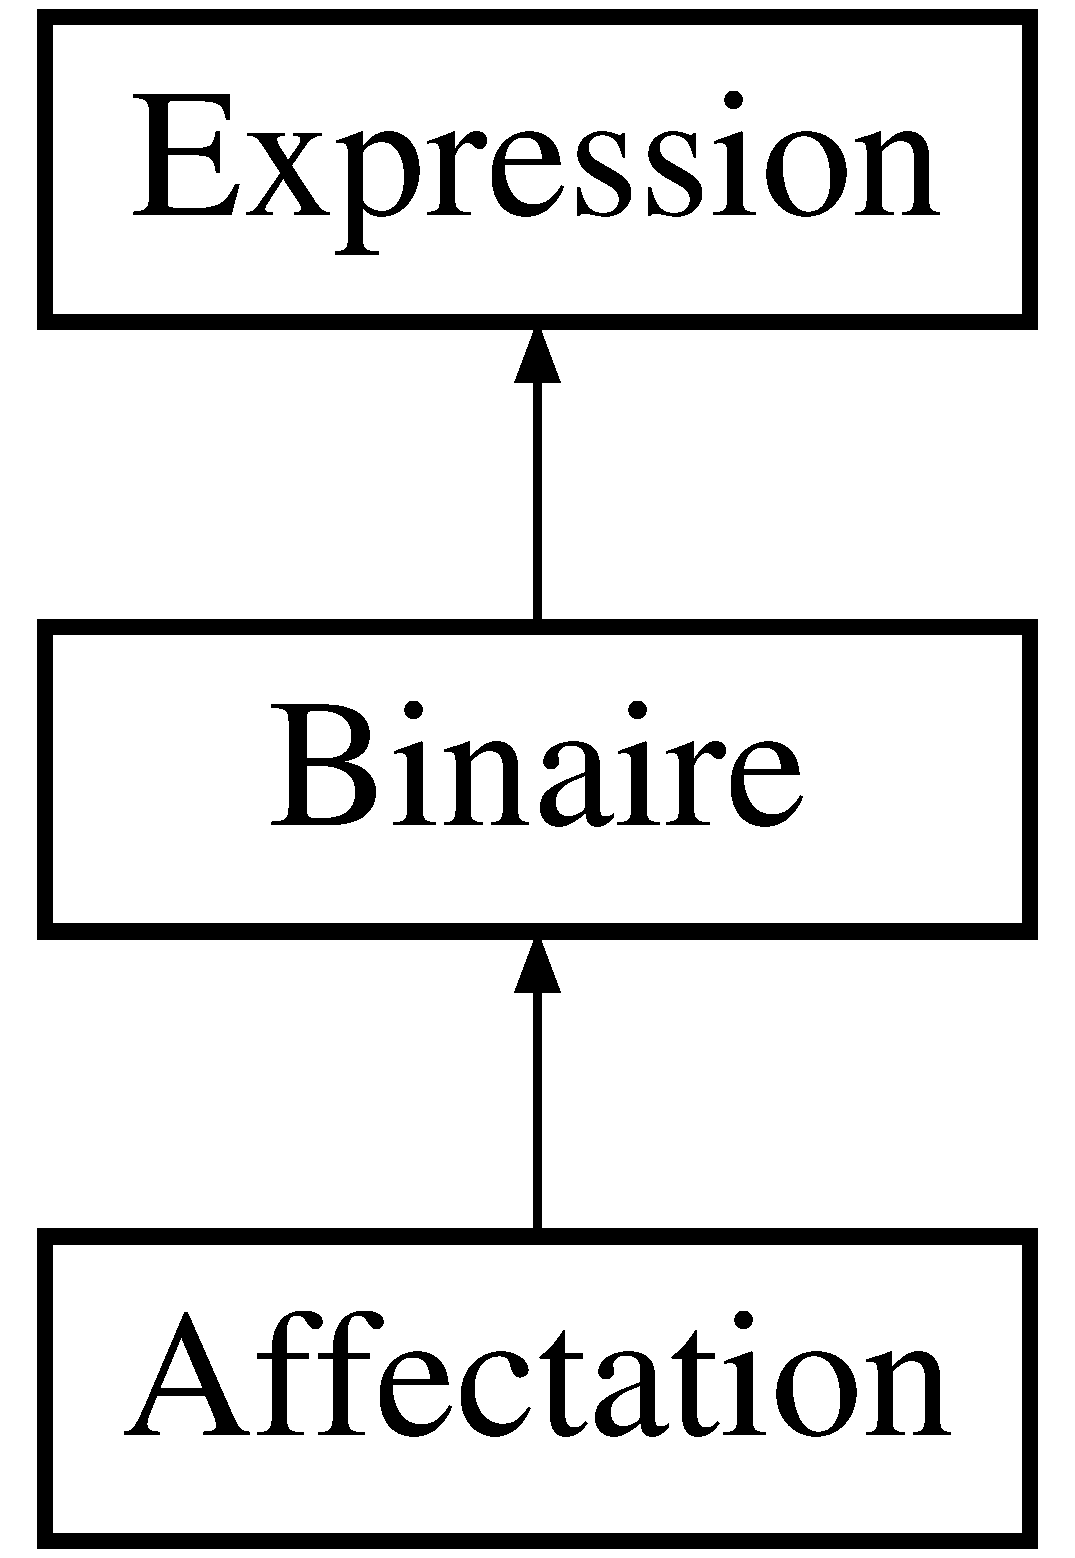
\includegraphics[height=3.000000cm]{class_affectation}
\end{center}
\end{figure}
\subsection*{Public Member Functions}
\begin{DoxyCompactItemize}
\item 
\hyperlink{class_affectation_a26f0693d0d5e4addca0df82fe3fd632e}{Affectation} ()
\begin{DoxyCompactList}\small\item\em Constructeur. \end{DoxyCompactList}\item 
\hyperlink{class_affectation_adf18b27ad9850ad779f16bc15bad57e5}{Affectation} (\hyperlink{class_variable}{Variable} $\ast$, \hyperlink{class_expression}{Expression} $\ast$)
\begin{DoxyCompactList}\small\item\em Constructeur. \end{DoxyCompactList}\item 
double \hyperlink{class_affectation_ad66950c792ad4ccf0e6491f55a7eaad2}{eval} () const 
\begin{DoxyCompactList}\small\item\em Evalue l\textquotesingle{}expression Methode qui permet d\textquotesingle{}evaluer l\textquotesingle{}expression. \end{DoxyCompactList}\item 
\hyperlink{class_expression}{Expression} $\ast$ \hyperlink{class_affectation_a918e2a05678e29ee1b7172e8eec95083}{deriver} (const string \&)
\begin{DoxyCompactList}\small\item\em Derive l\textquotesingle{}expression$\ast$ Methode qui permet deriver l\textquotesingle{}expression. \end{DoxyCompactList}\item 
\hyperlink{class_expression}{Expression} $\ast$ \hyperlink{class_affectation_ac39339edc60e2f44edf0cc8ec94e4313}{simplifier} ()
\begin{DoxyCompactList}\small\item\em Simplifie l\textquotesingle{}expression Methode qui permet de simplifier l\textquotesingle{}expression. \end{DoxyCompactList}\item 
virtual \hyperlink{class_affectation_a8fda35e6917179020490407736cd490d}{$\sim$\+Affectation} ()
\begin{DoxyCompactList}\small\item\em Destructeur Destructeur de la classe \hyperlink{class_affectation}{Affectation}. \end{DoxyCompactList}\item 
\hyperlink{class_expression}{Expression} $\ast$ \hyperlink{class_affectation_aef2d294e0ab788aace81d33097a80d18}{clone} () const 
\begin{DoxyCompactList}\small\item\em clone l\textquotesingle{}expression Methode qui permet de cloner l\textquotesingle{}expression \end{DoxyCompactList}\item 
string \hyperlink{class_affectation_a37acdac77acfb27d8c59abfdbd5ed3b0}{afficher} () const 
\begin{DoxyCompactList}\small\item\em Affiche l\textquotesingle{}expression Methode qui permet d\textquotesingle{}afficher l\textquotesingle{}expression. \end{DoxyCompactList}\end{DoxyCompactItemize}
\subsection*{Friends}
\begin{DoxyCompactItemize}
\item 
ostream \& \hyperlink{class_affectation_a88f8a9ffdfd76d32bb9a0dd742b283ac}{operator$<$$<$} (ostream \&os, const \hyperlink{class_affectation}{Affectation} \&affectation)
\begin{DoxyCompactList}\small\item\em operator$<$$<$ Methode qui permet d\textquotesingle{}afficher l\textquotesingle{}expression \end{DoxyCompactList}\end{DoxyCompactItemize}
\subsection*{Additional Inherited Members}


\subsection{Detailed Description}
La classe \hyperlink{class_affectation}{Affectation}. 

La classe permet d�affecter une valeur � une variable. Par exemple \+: x = 1, y = 2 

\subsection{Constructor \& Destructor Documentation}
\index{Affectation@{Affectation}!Affectation@{Affectation}}
\index{Affectation@{Affectation}!Affectation@{Affectation}}
\subsubsection[{\texorpdfstring{Affectation()}{Affectation()}}]{\setlength{\rightskip}{0pt plus 5cm}Affectation\+::\+Affectation (
\begin{DoxyParamCaption}
{}
\end{DoxyParamCaption}
)}\hypertarget{class_affectation_a26f0693d0d5e4addca0df82fe3fd632e}{}\label{class_affectation_a26f0693d0d5e4addca0df82fe3fd632e}


Constructeur. 

Constructeur de la classe \hyperlink{class_affectation}{Affectation} \index{Affectation@{Affectation}!Affectation@{Affectation}}
\index{Affectation@{Affectation}!Affectation@{Affectation}}
\subsubsection[{\texorpdfstring{Affectation(\+Variable $\ast$, Expression $\ast$)}{Affectation(Variable *, Expression *)}}]{\setlength{\rightskip}{0pt plus 5cm}Affectation\+::\+Affectation (
\begin{DoxyParamCaption}
\item[{{\bf Variable} $\ast$}]{variable, }
\item[{{\bf Expression} $\ast$}]{expression}
\end{DoxyParamCaption}
)}\hypertarget{class_affectation_adf18b27ad9850ad779f16bc15bad57e5}{}\label{class_affectation_adf18b27ad9850ad779f16bc15bad57e5}


Constructeur. 

Constructeur de la classe \hyperlink{class_affectation}{Affectation}


\begin{DoxyParams}{Parameters}
{\em variable} & \+: le variable \\
\hline
{\em valeur} & \+: le valeur \\
\hline
\end{DoxyParams}
\index{Affectation@{Affectation}!````~Affectation@{$\sim$\+Affectation}}
\index{````~Affectation@{$\sim$\+Affectation}!Affectation@{Affectation}}
\subsubsection[{\texorpdfstring{$\sim$\+Affectation()}{~Affectation()}}]{\setlength{\rightskip}{0pt plus 5cm}Affectation\+::$\sim$\+Affectation (
\begin{DoxyParamCaption}
{}
\end{DoxyParamCaption}
)\hspace{0.3cm}{\ttfamily [virtual]}}\hypertarget{class_affectation_a8fda35e6917179020490407736cd490d}{}\label{class_affectation_a8fda35e6917179020490407736cd490d}


Destructeur Destructeur de la classe \hyperlink{class_affectation}{Affectation}. 



\subsection{Member Function Documentation}
\index{Affectation@{Affectation}!afficher@{afficher}}
\index{afficher@{afficher}!Affectation@{Affectation}}
\subsubsection[{\texorpdfstring{afficher() const }{afficher() const }}]{\setlength{\rightskip}{0pt plus 5cm}string Affectation\+::afficher (
\begin{DoxyParamCaption}
{}
\end{DoxyParamCaption}
) const\hspace{0.3cm}{\ttfamily [virtual]}}\hypertarget{class_affectation_a37acdac77acfb27d8c59abfdbd5ed3b0}{}\label{class_affectation_a37acdac77acfb27d8c59abfdbd5ed3b0}


Affiche l\textquotesingle{}expression Methode qui permet d\textquotesingle{}afficher l\textquotesingle{}expression. 

\begin{DoxyReturn}{Returns}
Le string d\textquotesingle{}expression 
\end{DoxyReturn}


Reimplemented from \hyperlink{class_expression_a953c7de0302331023987a2fff895cb85}{Expression}.

\index{Affectation@{Affectation}!clone@{clone}}
\index{clone@{clone}!Affectation@{Affectation}}
\subsubsection[{\texorpdfstring{clone() const }{clone() const }}]{\setlength{\rightskip}{0pt plus 5cm}{\bf Expression} $\ast$ Affectation\+::clone (
\begin{DoxyParamCaption}
{}
\end{DoxyParamCaption}
) const\hspace{0.3cm}{\ttfamily [virtual]}}\hypertarget{class_affectation_aef2d294e0ab788aace81d33097a80d18}{}\label{class_affectation_aef2d294e0ab788aace81d33097a80d18}


clone l\textquotesingle{}expression Methode qui permet de cloner l\textquotesingle{}expression 

\begin{DoxyReturn}{Returns}
L\textquotesingle{}expression clon� 
\end{DoxyReturn}


Implements \hyperlink{class_expression_ac9fcea09ddd3a650a92c3606118abfb6}{Expression}.

\index{Affectation@{Affectation}!deriver@{deriver}}
\index{deriver@{deriver}!Affectation@{Affectation}}
\subsubsection[{\texorpdfstring{deriver(const string \&)}{deriver(const string &)}}]{\setlength{\rightskip}{0pt plus 5cm}{\bf Expression} $\ast$ Affectation\+::deriver (
\begin{DoxyParamCaption}
\item[{const string \&}]{var}
\end{DoxyParamCaption}
)\hspace{0.3cm}{\ttfamily [virtual]}}\hypertarget{class_affectation_a918e2a05678e29ee1b7172e8eec95083}{}\label{class_affectation_a918e2a05678e29ee1b7172e8eec95083}


Derive l\textquotesingle{}expression$\ast$ Methode qui permet deriver l\textquotesingle{}expression. 

\begin{DoxyReturn}{Returns}
L\textquotesingle{}expression deriv� 
\end{DoxyReturn}


Implements \hyperlink{class_expression_a0a2a2cf2cdb1e8ca556ad59832784193}{Expression}.

\index{Affectation@{Affectation}!eval@{eval}}
\index{eval@{eval}!Affectation@{Affectation}}
\subsubsection[{\texorpdfstring{eval() const }{eval() const }}]{\setlength{\rightskip}{0pt plus 5cm}double Affectation\+::eval (
\begin{DoxyParamCaption}
{}
\end{DoxyParamCaption}
) const\hspace{0.3cm}{\ttfamily [virtual]}}\hypertarget{class_affectation_ad66950c792ad4ccf0e6491f55a7eaad2}{}\label{class_affectation_ad66950c792ad4ccf0e6491f55a7eaad2}


Evalue l\textquotesingle{}expression Methode qui permet d\textquotesingle{}evaluer l\textquotesingle{}expression. 

\begin{DoxyReturn}{Returns}
Le valeur d\textquotesingle{}expression 
\end{DoxyReturn}


Implements \hyperlink{class_expression_a5481c36265e11eff513df87bbc5a1d33}{Expression}.

\index{Affectation@{Affectation}!simplifier@{simplifier}}
\index{simplifier@{simplifier}!Affectation@{Affectation}}
\subsubsection[{\texorpdfstring{simplifier()}{simplifier()}}]{\setlength{\rightskip}{0pt plus 5cm}{\bf Expression} $\ast$ Affectation\+::simplifier (
\begin{DoxyParamCaption}
{}
\end{DoxyParamCaption}
)\hspace{0.3cm}{\ttfamily [virtual]}}\hypertarget{class_affectation_ac39339edc60e2f44edf0cc8ec94e4313}{}\label{class_affectation_ac39339edc60e2f44edf0cc8ec94e4313}


Simplifie l\textquotesingle{}expression Methode qui permet de simplifier l\textquotesingle{}expression. 

\begin{DoxyReturn}{Returns}
L\textquotesingle{}expression simplifi� 
\end{DoxyReturn}


Implements \hyperlink{class_expression_a319d06d43ead325c835181419061ae0b}{Expression}.



\subsection{Friends And Related Function Documentation}
\index{Affectation@{Affectation}!operator$<$$<$@{operator$<$$<$}}
\index{operator$<$$<$@{operator$<$$<$}!Affectation@{Affectation}}
\subsubsection[{\texorpdfstring{operator$<$$<$}{operator<<}}]{\setlength{\rightskip}{0pt plus 5cm}ostream\& operator$<$$<$ (
\begin{DoxyParamCaption}
\item[{ostream \&}]{os, }
\item[{const {\bf Affectation} \&}]{affectation}
\end{DoxyParamCaption}
)\hspace{0.3cm}{\ttfamily [friend]}}\hypertarget{class_affectation_a88f8a9ffdfd76d32bb9a0dd742b283ac}{}\label{class_affectation_a88f8a9ffdfd76d32bb9a0dd742b283ac}


operator$<$$<$ Methode qui permet d\textquotesingle{}afficher l\textquotesingle{}expression 



The documentation for this class was generated from the following files\+:\begin{DoxyCompactItemize}
\item 
include/\hyperlink{affectation_8h}{affectation.\+h}\item 
src/\hyperlink{affectation_8cpp}{affectation.\+cpp}\end{DoxyCompactItemize}

\hypertarget{class_binaire}{}\section{Binaire Class Reference}
\label{class_binaire}\index{Binaire@{Binaire}}


La classe \hyperlink{class_binaire}{Binaire}.  




{\ttfamily \#include $<$binaire.\+h$>$}

Inheritance diagram for Binaire\+:\begin{figure}[H]
\begin{center}
\leavevmode
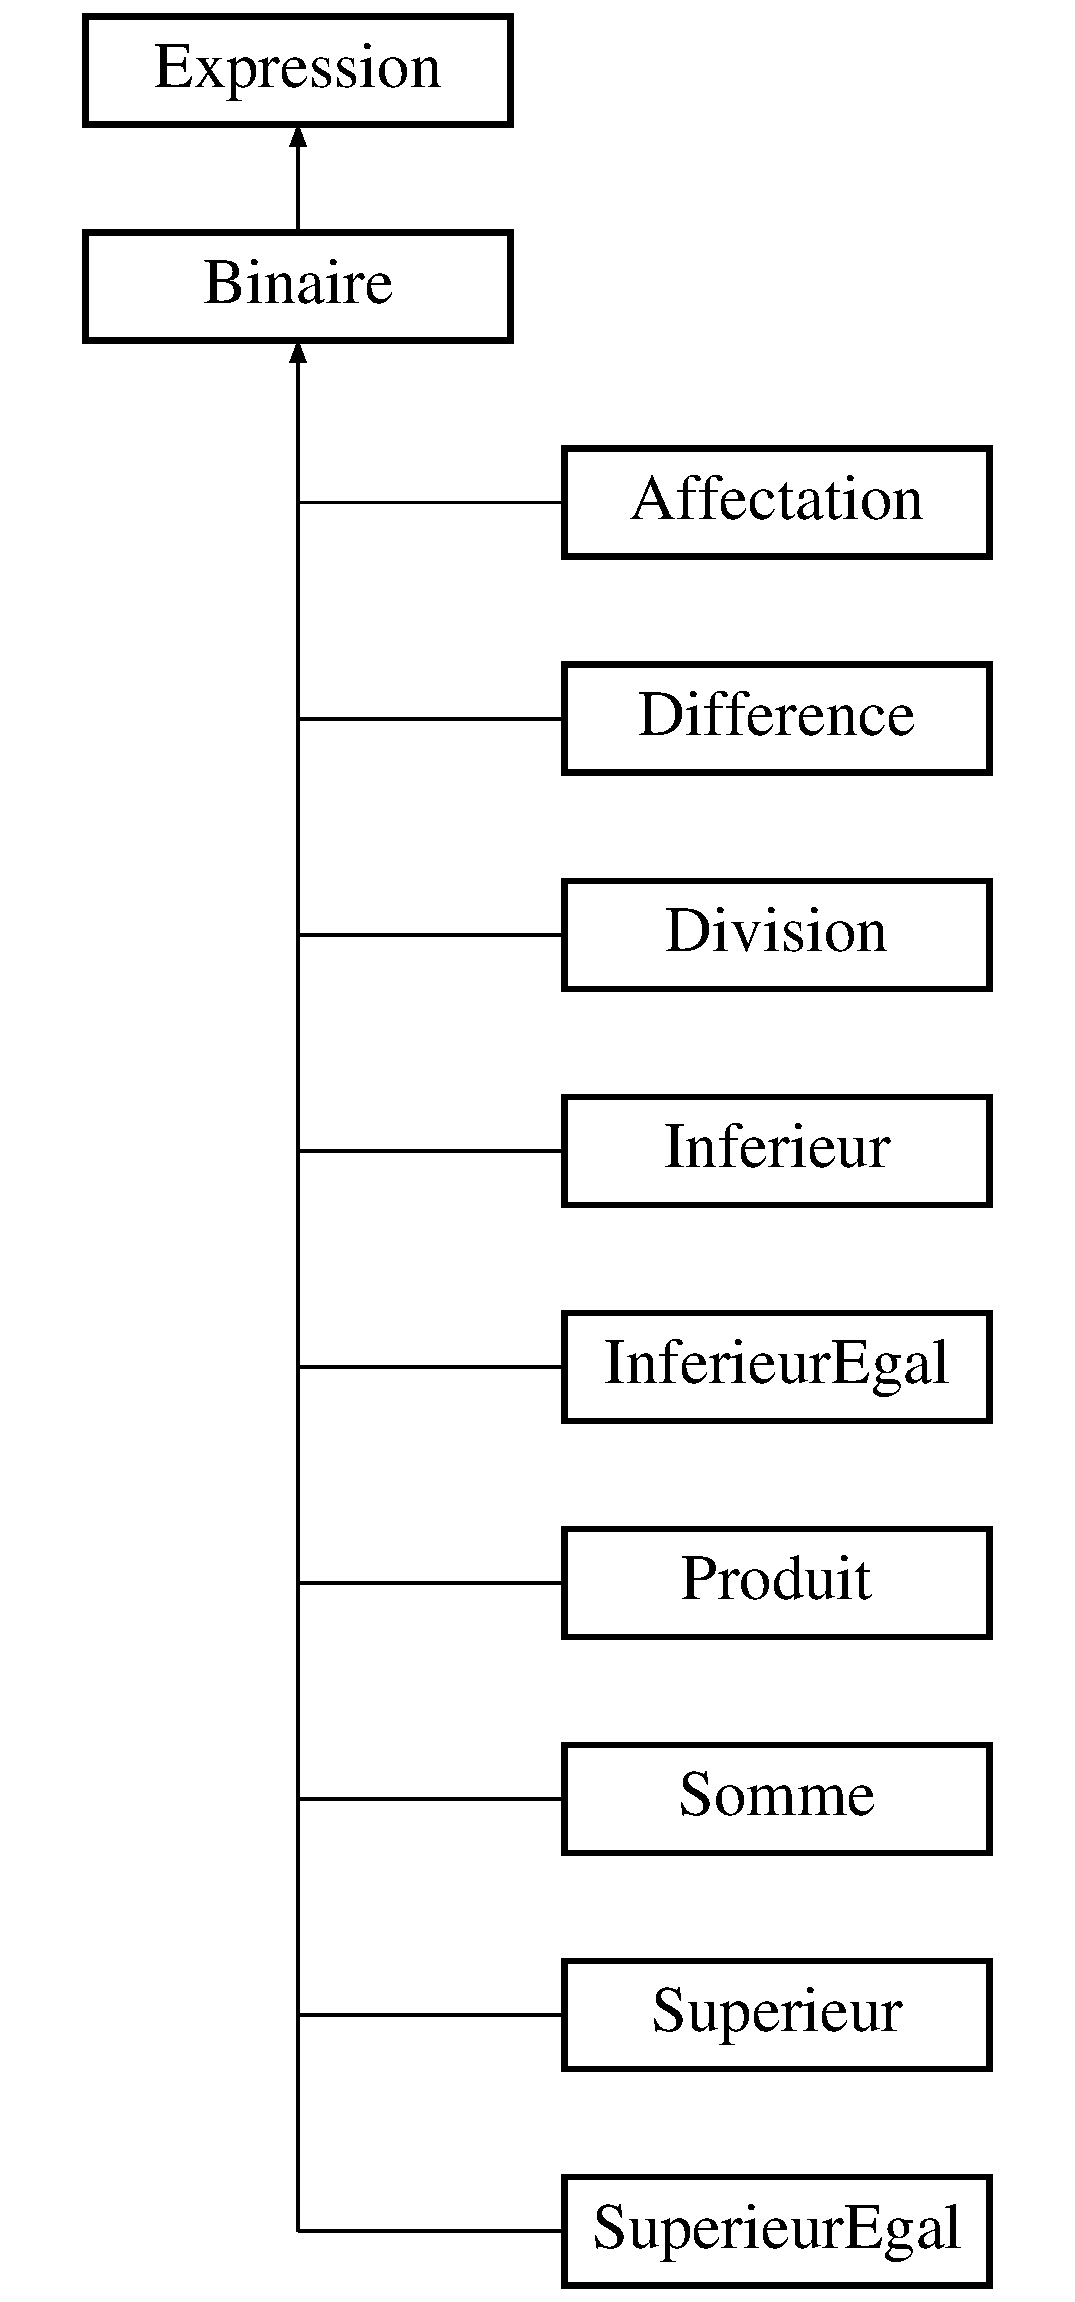
\includegraphics[height=11.000000cm]{class_binaire}
\end{center}
\end{figure}
\subsection*{Public Member Functions}
\begin{DoxyCompactItemize}
\item 
\hyperlink{class_binaire_a55dc843f26a41ec413ebfae828b12d6d}{Binaire} ()
\begin{DoxyCompactList}\small\item\em Constructeur. \end{DoxyCompactList}\item 
virtual \hyperlink{class_binaire_a7de31765437118a4f360fa751822e712}{$\sim$\+Binaire} ()
\begin{DoxyCompactList}\small\item\em Destructeur Destructeur de la classe \hyperlink{class_binaire}{Binaire}. \end{DoxyCompactList}\item 
\hyperlink{class_binaire_aa7a1ce136017a5b6d38d11dbfe24d730}{Binaire} (\hyperlink{class_expression}{Expression} $\ast$, \hyperlink{class_expression}{Expression} $\ast$, const string \&name=\char`\"{}binaire\char`\"{})
\begin{DoxyCompactList}\small\item\em Constructeur. \end{DoxyCompactList}\item 
virtual string \hyperlink{class_binaire_a0efae1967f81c3c9dba27cd5a7bca324}{afficher} ()
\begin{DoxyCompactList}\small\item\em Affiche l\textquotesingle{}expression Methode qui permet d\textquotesingle{}afficher l\textquotesingle{}expression. \end{DoxyCompactList}\end{DoxyCompactItemize}
\subsection*{Protected Attributes}
\begin{DoxyCompactItemize}
\item 
\hyperlink{class_expression}{Expression} $\ast$ \hyperlink{class_binaire_a6edcd547ab6cf6f0030920fa3c8b0109}{\+\_\+gauche}
\item 
\hyperlink{class_expression}{Expression} $\ast$ \hyperlink{class_binaire_a3f2040ac9dc51e90388407032c4603cf}{\+\_\+droite}
\end{DoxyCompactItemize}
\subsection*{Additional Inherited Members}


\subsection{Detailed Description}
La classe \hyperlink{class_binaire}{Binaire}. 

Cette classe repr�sente les op�rateurs binaires 

\subsection{Constructor \& Destructor Documentation}
\index{Binaire@{Binaire}!Binaire@{Binaire}}
\index{Binaire@{Binaire}!Binaire@{Binaire}}
\subsubsection[{\texorpdfstring{Binaire()}{Binaire()}}]{\setlength{\rightskip}{0pt plus 5cm}Binaire\+::\+Binaire (
\begin{DoxyParamCaption}
{}
\end{DoxyParamCaption}
)}\hypertarget{class_binaire_a55dc843f26a41ec413ebfae828b12d6d}{}\label{class_binaire_a55dc843f26a41ec413ebfae828b12d6d}


Constructeur. 

Constructeur de la classe \hyperlink{class_binaire}{Binaire} \index{Binaire@{Binaire}!````~Binaire@{$\sim$\+Binaire}}
\index{````~Binaire@{$\sim$\+Binaire}!Binaire@{Binaire}}
\subsubsection[{\texorpdfstring{$\sim$\+Binaire()}{~Binaire()}}]{\setlength{\rightskip}{0pt plus 5cm}Binaire\+::$\sim$\+Binaire (
\begin{DoxyParamCaption}
{}
\end{DoxyParamCaption}
)\hspace{0.3cm}{\ttfamily [virtual]}}\hypertarget{class_binaire_a7de31765437118a4f360fa751822e712}{}\label{class_binaire_a7de31765437118a4f360fa751822e712}


Destructeur Destructeur de la classe \hyperlink{class_binaire}{Binaire}. 

\index{Binaire@{Binaire}!Binaire@{Binaire}}
\index{Binaire@{Binaire}!Binaire@{Binaire}}
\subsubsection[{\texorpdfstring{Binaire(\+Expression $\ast$, Expression $\ast$, const string \&name=""binaire"")}{Binaire(Expression *, Expression *, const string &name="binaire")}}]{\setlength{\rightskip}{0pt plus 5cm}Binaire\+::\+Binaire (
\begin{DoxyParamCaption}
\item[{{\bf Expression} $\ast$}]{op1, }
\item[{{\bf Expression} $\ast$}]{op2, }
\item[{const string \&}]{name = {\ttfamily \char`\"{}binaire\char`\"{}}}
\end{DoxyParamCaption}
)}\hypertarget{class_binaire_aa7a1ce136017a5b6d38d11dbfe24d730}{}\label{class_binaire_aa7a1ce136017a5b6d38d11dbfe24d730}


Constructeur. 

Constructeur de la classe \hyperlink{class_binaire}{Binaire}


\begin{DoxyParams}{Parameters}
{\em exp1} & \+: op�rande gauche \\
\hline
{\em exp2} & \+: op�rande droite \\
\hline
\end{DoxyParams}


\subsection{Member Function Documentation}
\index{Binaire@{Binaire}!afficher@{afficher}}
\index{afficher@{afficher}!Binaire@{Binaire}}
\subsubsection[{\texorpdfstring{afficher()}{afficher()}}]{\setlength{\rightskip}{0pt plus 5cm}string Binaire\+::afficher (
\begin{DoxyParamCaption}
{}
\end{DoxyParamCaption}
)\hspace{0.3cm}{\ttfamily [virtual]}}\hypertarget{class_binaire_a0efae1967f81c3c9dba27cd5a7bca324}{}\label{class_binaire_a0efae1967f81c3c9dba27cd5a7bca324}


Affiche l\textquotesingle{}expression Methode qui permet d\textquotesingle{}afficher l\textquotesingle{}expression. 

\begin{DoxyReturn}{Returns}
Le string d\textquotesingle{}expression 
\end{DoxyReturn}


\subsection{Member Data Documentation}
\index{Binaire@{Binaire}!\+\_\+droite@{\+\_\+droite}}
\index{\+\_\+droite@{\+\_\+droite}!Binaire@{Binaire}}
\subsubsection[{\texorpdfstring{\+\_\+droite}{_droite}}]{\setlength{\rightskip}{0pt plus 5cm}{\bf Expression} $\ast$ Binaire\+::\+\_\+droite\hspace{0.3cm}{\ttfamily [protected]}}\hypertarget{class_binaire_a3f2040ac9dc51e90388407032c4603cf}{}\label{class_binaire_a3f2040ac9dc51e90388407032c4603cf}
\index{Binaire@{Binaire}!\+\_\+gauche@{\+\_\+gauche}}
\index{\+\_\+gauche@{\+\_\+gauche}!Binaire@{Binaire}}
\subsubsection[{\texorpdfstring{\+\_\+gauche}{_gauche}}]{\setlength{\rightskip}{0pt plus 5cm}{\bf Expression}$\ast$ Binaire\+::\+\_\+gauche\hspace{0.3cm}{\ttfamily [protected]}}\hypertarget{class_binaire_a6edcd547ab6cf6f0030920fa3c8b0109}{}\label{class_binaire_a6edcd547ab6cf6f0030920fa3c8b0109}


The documentation for this class was generated from the following files\+:\begin{DoxyCompactItemize}
\item 
include/\hyperlink{binaire_8h}{binaire.\+h}\item 
src/\hyperlink{binaire_8cpp}{binaire.\+cpp}\end{DoxyCompactItemize}

\hypertarget{class_bloc}{}\section{Bloc Class Reference}
\label{class_bloc}\index{Bloc@{Bloc}}


La classe \hyperlink{class_bloc}{Bloc}.  




{\ttfamily \#include $<$bloc.\+h$>$}

Inheritance diagram for Bloc\+:\begin{figure}[H]
\begin{center}
\leavevmode
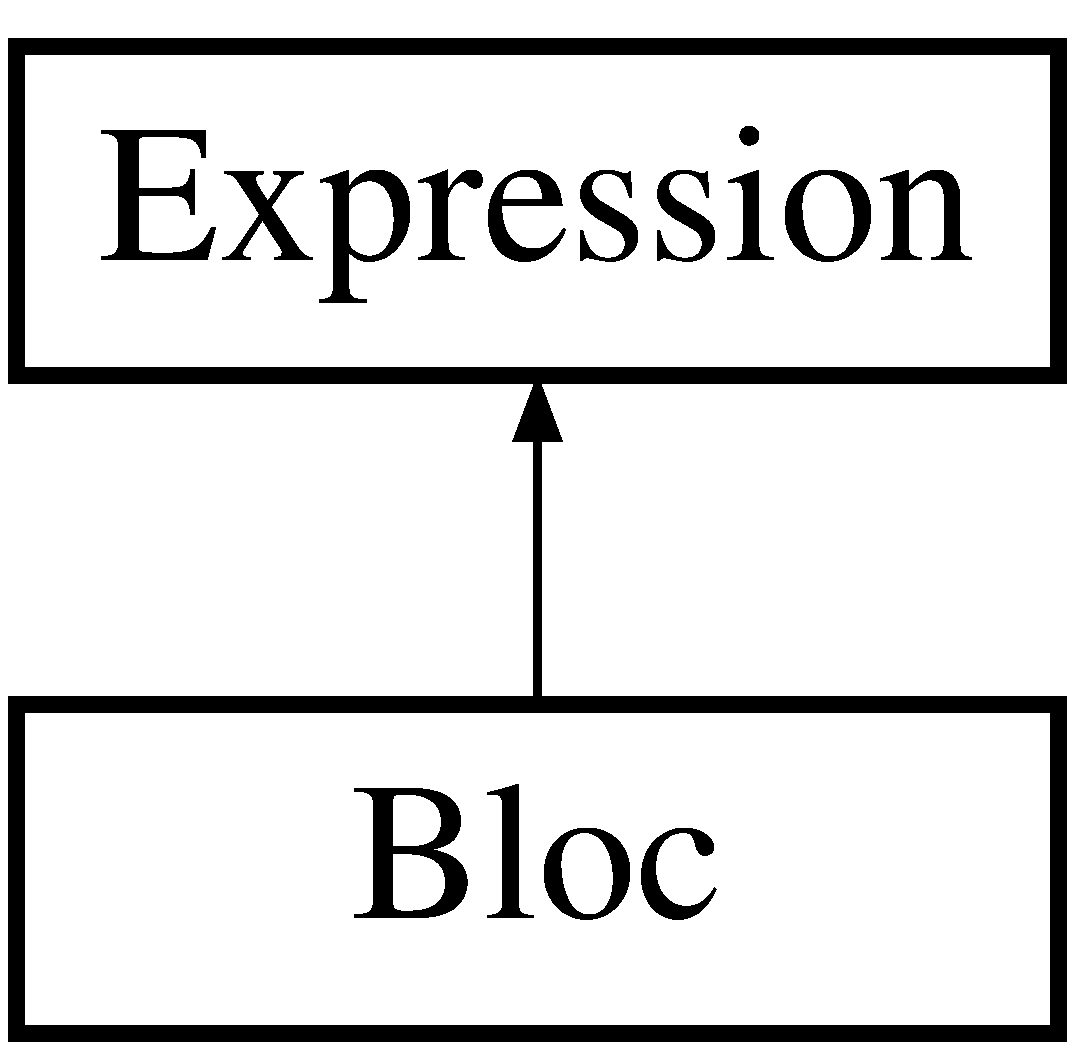
\includegraphics[height=2.000000cm]{class_bloc}
\end{center}
\end{figure}
\subsection*{Public Member Functions}
\begin{DoxyCompactItemize}
\item 
\hyperlink{class_bloc_ae3ac5cbad6363c4ab56262a94d0b982e}{Bloc} ()
\begin{DoxyCompactList}\small\item\em Constructeur. \end{DoxyCompactList}\item 
virtual \hyperlink{class_bloc_a1f40a68b1acb741fc91e07bbaa61dc22}{$\sim$\+Bloc} ()
\begin{DoxyCompactList}\small\item\em Destructeur Destructeur de la classe \hyperlink{class_affectation}{Affectation}. \end{DoxyCompactList}\item 
\hyperlink{class_bloc_aabf8e5cb40aa177dfb12ebc79e9a2550}{Bloc} (const string \&, \hyperlink{class_expression}{Expression} $\ast$)
\begin{DoxyCompactList}\small\item\em Constructeur. \end{DoxyCompactList}\item 
\hyperlink{class_expression}{Expression} $\ast$ \hyperlink{class_bloc_a15c01c71bdad5b42c2d79102a19ca5aa}{clone} () const 
\begin{DoxyCompactList}\small\item\em clone l\textquotesingle{}expression Methode qui permet de cloner l\textquotesingle{}expression \end{DoxyCompactList}\item 
string \hyperlink{class_bloc_acfe2075a0f69de800f447c1bc0aee63f}{afficher} () const 
\begin{DoxyCompactList}\small\item\em Affiche l\textquotesingle{}expression Methode qui permet d\textquotesingle{}afficher l\textquotesingle{}expression. \end{DoxyCompactList}\item 
double \hyperlink{class_bloc_a8847a4df7adf319e48ed7a277347ac80}{eval} () const 
\begin{DoxyCompactList}\small\item\em Evalue l\textquotesingle{}expression Methode qui permet d\textquotesingle{}evaluer l\textquotesingle{}expression. \end{DoxyCompactList}\item 
\hyperlink{class_expression}{Expression} $\ast$ \hyperlink{class_bloc_ad8547a697be0d0829fbf13d4f6623376}{deriver} (const string \&)
\begin{DoxyCompactList}\small\item\em Derive l\textquotesingle{}expression$\ast$ Methode qui permet deriver l\textquotesingle{}expression. \end{DoxyCompactList}\item 
\hyperlink{class_expression}{Expression} $\ast$ \hyperlink{class_bloc_afd5d437c0b31109b90946d183a150642}{simplifier} ()
\begin{DoxyCompactList}\small\item\em Simplifie l\textquotesingle{}expression Methode qui permet de simplifier l\textquotesingle{}expression. \end{DoxyCompactList}\item 
void \hyperlink{class_bloc_ab3698ded3f7a5765c15f0f18a2ce5e13}{add} (\hyperlink{class_expression}{Expression} $\ast$)
\end{DoxyCompactItemize}
\subsection*{Friends}
\begin{DoxyCompactItemize}
\item 
ostream \& \hyperlink{class_bloc_a3154373e6bca7fa42a1832b56f4681fa}{operator$<$$<$} (ostream \&os, const \hyperlink{class_bloc}{Bloc} \&)
\begin{DoxyCompactList}\small\item\em operator$<$$<$ Methode qui permet d\textquotesingle{}afficher l\textquotesingle{}expression \end{DoxyCompactList}\end{DoxyCompactItemize}
\subsection*{Additional Inherited Members}


\subsection{Detailed Description}
La classe \hyperlink{class_bloc}{Bloc}. 

Cette classe repr�sente une s�quence d�instructions (expression) sur le m�me mod�le 

\subsection{Constructor \& Destructor Documentation}
\index{Bloc@{Bloc}!Bloc@{Bloc}}
\index{Bloc@{Bloc}!Bloc@{Bloc}}
\subsubsection[{\texorpdfstring{Bloc()}{Bloc()}}]{\setlength{\rightskip}{0pt plus 5cm}Bloc\+::\+Bloc (
\begin{DoxyParamCaption}
{}
\end{DoxyParamCaption}
)}\hypertarget{class_bloc_ae3ac5cbad6363c4ab56262a94d0b982e}{}\label{class_bloc_ae3ac5cbad6363c4ab56262a94d0b982e}


Constructeur. 

Constructeur de la classe \hyperlink{class_bloc}{Bloc} \index{Bloc@{Bloc}!````~Bloc@{$\sim$\+Bloc}}
\index{````~Bloc@{$\sim$\+Bloc}!Bloc@{Bloc}}
\subsubsection[{\texorpdfstring{$\sim$\+Bloc()}{~Bloc()}}]{\setlength{\rightskip}{0pt plus 5cm}Bloc\+::$\sim$\+Bloc (
\begin{DoxyParamCaption}
{}
\end{DoxyParamCaption}
)\hspace{0.3cm}{\ttfamily [virtual]}}\hypertarget{class_bloc_a1f40a68b1acb741fc91e07bbaa61dc22}{}\label{class_bloc_a1f40a68b1acb741fc91e07bbaa61dc22}


Destructeur Destructeur de la classe \hyperlink{class_affectation}{Affectation}. 

\index{Bloc@{Bloc}!Bloc@{Bloc}}
\index{Bloc@{Bloc}!Bloc@{Bloc}}
\subsubsection[{\texorpdfstring{Bloc(const string \&, Expression $\ast$)}{Bloc(const string &, Expression *)}}]{\setlength{\rightskip}{0pt plus 5cm}Bloc\+::\+Bloc (
\begin{DoxyParamCaption}
\item[{const string \&}]{nom, }
\item[{{\bf Expression} $\ast$}]{exp1}
\end{DoxyParamCaption}
)}\hypertarget{class_bloc_aabf8e5cb40aa177dfb12ebc79e9a2550}{}\label{class_bloc_aabf8e5cb40aa177dfb12ebc79e9a2550}


Constructeur. 

Constructeur de la classe \hyperlink{class_bloc}{Bloc}


\begin{DoxyParams}{Parameters}
{\em nom} & \+: nom du bloc \\
\hline
{\em expression} & \+: l\textquotesingle{}expression \\
\hline
\end{DoxyParams}


\subsection{Member Function Documentation}
\index{Bloc@{Bloc}!add@{add}}
\index{add@{add}!Bloc@{Bloc}}
\subsubsection[{\texorpdfstring{add(\+Expression $\ast$)}{add(Expression *)}}]{\setlength{\rightskip}{0pt plus 5cm}void Bloc\+::add (
\begin{DoxyParamCaption}
\item[{{\bf Expression} $\ast$}]{expression}
\end{DoxyParamCaption}
)}\hypertarget{class_bloc_ab3698ded3f7a5765c15f0f18a2ce5e13}{}\label{class_bloc_ab3698ded3f7a5765c15f0f18a2ce5e13}
\index{Bloc@{Bloc}!afficher@{afficher}}
\index{afficher@{afficher}!Bloc@{Bloc}}
\subsubsection[{\texorpdfstring{afficher() const }{afficher() const }}]{\setlength{\rightskip}{0pt plus 5cm}string Bloc\+::afficher (
\begin{DoxyParamCaption}
{}
\end{DoxyParamCaption}
) const\hspace{0.3cm}{\ttfamily [virtual]}}\hypertarget{class_bloc_acfe2075a0f69de800f447c1bc0aee63f}{}\label{class_bloc_acfe2075a0f69de800f447c1bc0aee63f}


Affiche l\textquotesingle{}expression Methode qui permet d\textquotesingle{}afficher l\textquotesingle{}expression. 

\begin{DoxyReturn}{Returns}
Le string d\textquotesingle{}expression 
\end{DoxyReturn}


Reimplemented from \hyperlink{class_expression_a953c7de0302331023987a2fff895cb85}{Expression}.

\index{Bloc@{Bloc}!clone@{clone}}
\index{clone@{clone}!Bloc@{Bloc}}
\subsubsection[{\texorpdfstring{clone() const }{clone() const }}]{\setlength{\rightskip}{0pt plus 5cm}{\bf Expression} $\ast$ Bloc\+::clone (
\begin{DoxyParamCaption}
{}
\end{DoxyParamCaption}
) const\hspace{0.3cm}{\ttfamily [virtual]}}\hypertarget{class_bloc_a15c01c71bdad5b42c2d79102a19ca5aa}{}\label{class_bloc_a15c01c71bdad5b42c2d79102a19ca5aa}


clone l\textquotesingle{}expression Methode qui permet de cloner l\textquotesingle{}expression 

\begin{DoxyReturn}{Returns}
L\textquotesingle{}expression clon� 
\end{DoxyReturn}


Implements \hyperlink{class_expression_ac9fcea09ddd3a650a92c3606118abfb6}{Expression}.

\index{Bloc@{Bloc}!deriver@{deriver}}
\index{deriver@{deriver}!Bloc@{Bloc}}
\subsubsection[{\texorpdfstring{deriver(const string \&)}{deriver(const string &)}}]{\setlength{\rightskip}{0pt plus 5cm}{\bf Expression} $\ast$ Bloc\+::deriver (
\begin{DoxyParamCaption}
\item[{const string \&}]{var}
\end{DoxyParamCaption}
)\hspace{0.3cm}{\ttfamily [virtual]}}\hypertarget{class_bloc_ad8547a697be0d0829fbf13d4f6623376}{}\label{class_bloc_ad8547a697be0d0829fbf13d4f6623376}


Derive l\textquotesingle{}expression$\ast$ Methode qui permet deriver l\textquotesingle{}expression. 

\begin{DoxyReturn}{Returns}
L\textquotesingle{}expression deriv� 
\end{DoxyReturn}


Implements \hyperlink{class_expression_a0a2a2cf2cdb1e8ca556ad59832784193}{Expression}.

\index{Bloc@{Bloc}!eval@{eval}}
\index{eval@{eval}!Bloc@{Bloc}}
\subsubsection[{\texorpdfstring{eval() const }{eval() const }}]{\setlength{\rightskip}{0pt plus 5cm}double Bloc\+::eval (
\begin{DoxyParamCaption}
{}
\end{DoxyParamCaption}
) const\hspace{0.3cm}{\ttfamily [virtual]}}\hypertarget{class_bloc_a8847a4df7adf319e48ed7a277347ac80}{}\label{class_bloc_a8847a4df7adf319e48ed7a277347ac80}


Evalue l\textquotesingle{}expression Methode qui permet d\textquotesingle{}evaluer l\textquotesingle{}expression. 

\begin{DoxyReturn}{Returns}
Le valeur d\textquotesingle{}expression 
\end{DoxyReturn}


Implements \hyperlink{class_expression_a5481c36265e11eff513df87bbc5a1d33}{Expression}.

\index{Bloc@{Bloc}!simplifier@{simplifier}}
\index{simplifier@{simplifier}!Bloc@{Bloc}}
\subsubsection[{\texorpdfstring{simplifier()}{simplifier()}}]{\setlength{\rightskip}{0pt plus 5cm}{\bf Expression} $\ast$ Bloc\+::simplifier (
\begin{DoxyParamCaption}
{}
\end{DoxyParamCaption}
)\hspace{0.3cm}{\ttfamily [virtual]}}\hypertarget{class_bloc_afd5d437c0b31109b90946d183a150642}{}\label{class_bloc_afd5d437c0b31109b90946d183a150642}


Simplifie l\textquotesingle{}expression Methode qui permet de simplifier l\textquotesingle{}expression. 

\begin{DoxyReturn}{Returns}
L\textquotesingle{}expression simplifi� 
\end{DoxyReturn}


Implements \hyperlink{class_expression_a319d06d43ead325c835181419061ae0b}{Expression}.



\subsection{Friends And Related Function Documentation}
\index{Bloc@{Bloc}!operator$<$$<$@{operator$<$$<$}}
\index{operator$<$$<$@{operator$<$$<$}!Bloc@{Bloc}}
\subsubsection[{\texorpdfstring{operator$<$$<$}{operator<<}}]{\setlength{\rightskip}{0pt plus 5cm}ostream\& operator$<$$<$ (
\begin{DoxyParamCaption}
\item[{ostream \&}]{os, }
\item[{const {\bf Bloc} \&}]{bloc}
\end{DoxyParamCaption}
)\hspace{0.3cm}{\ttfamily [friend]}}\hypertarget{class_bloc_a3154373e6bca7fa42a1832b56f4681fa}{}\label{class_bloc_a3154373e6bca7fa42a1832b56f4681fa}


operator$<$$<$ Methode qui permet d\textquotesingle{}afficher l\textquotesingle{}expression 



The documentation for this class was generated from the following files\+:\begin{DoxyCompactItemize}
\item 
include/\hyperlink{bloc_8h}{bloc.\+h}\item 
src/\hyperlink{bloc_8cpp}{bloc.\+cpp}\end{DoxyCompactItemize}

\hypertarget{class_conditionnel}{}\section{Conditionnel Class Reference}
\label{class_conditionnel}\index{Conditionnel@{Conditionnel}}


La classe \hyperlink{class_conditionnel}{Conditionnel}.  




{\ttfamily \#include $<$conditionnel.\+h$>$}

Inheritance diagram for Conditionnel\+:\begin{figure}[H]
\begin{center}
\leavevmode
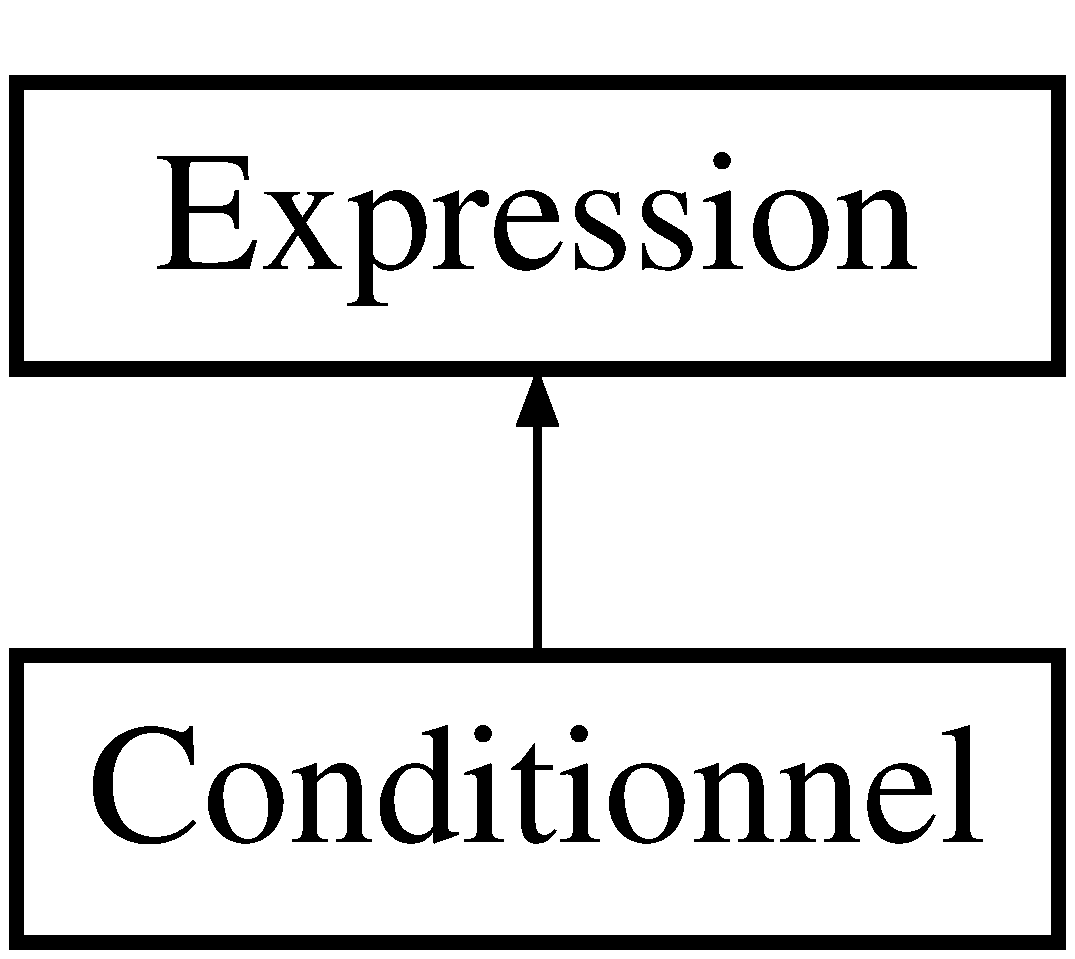
\includegraphics[height=2.000000cm]{class_conditionnel}
\end{center}
\end{figure}
\subsection*{Public Member Functions}
\begin{DoxyCompactItemize}
\item 
\hyperlink{class_conditionnel_a850d4e1a18d5bd594d525e7cfa6f2852}{Conditionnel} ()
\begin{DoxyCompactList}\small\item\em Constructeur. \end{DoxyCompactList}\item 
\hyperlink{class_conditionnel_ac6691d368ba09e30c379c3e21978bc87}{Conditionnel} (\hyperlink{class_binaire}{Binaire} $\ast$, \hyperlink{class_expression}{Expression} $\ast$, \hyperlink{class_expression}{Expression} $\ast$)
\begin{DoxyCompactList}\small\item\em Constructeur. \end{DoxyCompactList}\item 
virtual \hyperlink{class_conditionnel_a0438817d80fc5fc36f1bb0fac869aa33}{$\sim$\+Conditionnel} ()
\begin{DoxyCompactList}\small\item\em Destructeur Destructeur de la classe \hyperlink{class_affectation}{Affectation}. \end{DoxyCompactList}\item 
\hyperlink{class_expression}{Expression} $\ast$ \hyperlink{class_conditionnel_a3dec2cad7a9a43495c4bdc2b6b65f4a4}{clone} () const 
\begin{DoxyCompactList}\small\item\em clone l\textquotesingle{}expression Methode qui permet de cloner l\textquotesingle{}expression \end{DoxyCompactList}\item 
string \hyperlink{class_conditionnel_ace6f0a27597c614b82a0f84a329167cf}{afficher} () const 
\begin{DoxyCompactList}\small\item\em Affiche l\textquotesingle{}expression Methode qui permet d\textquotesingle{}afficher l\textquotesingle{}expression. \end{DoxyCompactList}\item 
double \hyperlink{class_conditionnel_a1421ef0258647e5c85a1fb2dc8a9434f}{eval} () const 
\begin{DoxyCompactList}\small\item\em Evalue l\textquotesingle{}expression Methode qui permet d\textquotesingle{}evaluer l\textquotesingle{}expression. \end{DoxyCompactList}\item 
\hyperlink{class_expression}{Expression} $\ast$ \hyperlink{class_conditionnel_ac7ac864a499c05d874ab88dbb4bda442}{deriver} (const string \&)
\begin{DoxyCompactList}\small\item\em Derive l\textquotesingle{}expression$\ast$ Methode qui permet deriver l\textquotesingle{}expression. \end{DoxyCompactList}\item 
\hyperlink{class_expression}{Expression} $\ast$ \hyperlink{class_conditionnel_adafd38733d1384a44f981a292f234e1f}{simplifier} ()
\begin{DoxyCompactList}\small\item\em Simplifie l\textquotesingle{}expression Methode qui permet de simplifier l\textquotesingle{}expression. \end{DoxyCompactList}\end{DoxyCompactItemize}
\subsection*{Friends}
\begin{DoxyCompactItemize}
\item 
ostream \& \hyperlink{class_conditionnel_a4232dfc0051fa6dc07b1bf61879eaef7}{operator$<$$<$} (ostream \&os, const \hyperlink{class_conditionnel}{Conditionnel} \&)
\begin{DoxyCompactList}\small\item\em operator$<$$<$ Methode qui permet d\textquotesingle{}afficher l\textquotesingle{}expression \end{DoxyCompactList}\end{DoxyCompactItemize}
\subsection*{Additional Inherited Members}


\subsection{Detailed Description}
La classe \hyperlink{class_conditionnel}{Conditionnel}. 

Cette classe repr�sente les op�rateurs ternaire. Elles permettent d\textquotesingle{}obtenir une valeur si une condition est vraie, et une autre si la condition est fausse. Ils ont de forme \+: (cond)?e1\+:e2 

\subsection{Constructor \& Destructor Documentation}
\index{Conditionnel@{Conditionnel}!Conditionnel@{Conditionnel}}
\index{Conditionnel@{Conditionnel}!Conditionnel@{Conditionnel}}
\subsubsection[{\texorpdfstring{Conditionnel()}{Conditionnel()}}]{\setlength{\rightskip}{0pt plus 5cm}Conditionnel\+::\+Conditionnel (
\begin{DoxyParamCaption}
{}
\end{DoxyParamCaption}
)}\hypertarget{class_conditionnel_a850d4e1a18d5bd594d525e7cfa6f2852}{}\label{class_conditionnel_a850d4e1a18d5bd594d525e7cfa6f2852}


Constructeur. 

Constructeur de la classe \hyperlink{class_conditionnel}{Conditionnel} \index{Conditionnel@{Conditionnel}!Conditionnel@{Conditionnel}}
\index{Conditionnel@{Conditionnel}!Conditionnel@{Conditionnel}}
\subsubsection[{\texorpdfstring{Conditionnel(\+Binaire $\ast$, Expression $\ast$, Expression $\ast$)}{Conditionnel(Binaire *, Expression *, Expression *)}}]{\setlength{\rightskip}{0pt plus 5cm}Conditionnel\+::\+Conditionnel (
\begin{DoxyParamCaption}
\item[{{\bf Binaire} $\ast$}]{cond, }
\item[{{\bf Expression} $\ast$}]{exp1, }
\item[{{\bf Expression} $\ast$}]{exp2}
\end{DoxyParamCaption}
)}\hypertarget{class_conditionnel_ac6691d368ba09e30c379c3e21978bc87}{}\label{class_conditionnel_ac6691d368ba09e30c379c3e21978bc87}


Constructeur. 

Constructeur de la classe \hyperlink{class_conditionnel}{Conditionnel}


\begin{DoxyParams}{Parameters}
{\em cond} & \+: la condition \\
\hline
{\em exp1} & \+: l\textquotesingle{}expression si la condition est vraie \\
\hline
{\em exp2} & \+: l\textquotesingle{}expression si la condition est fausse \\
\hline
\end{DoxyParams}
\index{Conditionnel@{Conditionnel}!````~Conditionnel@{$\sim$\+Conditionnel}}
\index{````~Conditionnel@{$\sim$\+Conditionnel}!Conditionnel@{Conditionnel}}
\subsubsection[{\texorpdfstring{$\sim$\+Conditionnel()}{~Conditionnel()}}]{\setlength{\rightskip}{0pt plus 5cm}Conditionnel\+::$\sim$\+Conditionnel (
\begin{DoxyParamCaption}
{}
\end{DoxyParamCaption}
)\hspace{0.3cm}{\ttfamily [virtual]}}\hypertarget{class_conditionnel_a0438817d80fc5fc36f1bb0fac869aa33}{}\label{class_conditionnel_a0438817d80fc5fc36f1bb0fac869aa33}


Destructeur Destructeur de la classe \hyperlink{class_affectation}{Affectation}. 



\subsection{Member Function Documentation}
\index{Conditionnel@{Conditionnel}!afficher@{afficher}}
\index{afficher@{afficher}!Conditionnel@{Conditionnel}}
\subsubsection[{\texorpdfstring{afficher() const }{afficher() const }}]{\setlength{\rightskip}{0pt plus 5cm}string Conditionnel\+::afficher (
\begin{DoxyParamCaption}
{}
\end{DoxyParamCaption}
) const\hspace{0.3cm}{\ttfamily [virtual]}}\hypertarget{class_conditionnel_ace6f0a27597c614b82a0f84a329167cf}{}\label{class_conditionnel_ace6f0a27597c614b82a0f84a329167cf}


Affiche l\textquotesingle{}expression Methode qui permet d\textquotesingle{}afficher l\textquotesingle{}expression. 

\begin{DoxyReturn}{Returns}
Le string d\textquotesingle{}expression 
\end{DoxyReturn}


Reimplemented from \hyperlink{class_expression_a953c7de0302331023987a2fff895cb85}{Expression}.

\index{Conditionnel@{Conditionnel}!clone@{clone}}
\index{clone@{clone}!Conditionnel@{Conditionnel}}
\subsubsection[{\texorpdfstring{clone() const }{clone() const }}]{\setlength{\rightskip}{0pt plus 5cm}{\bf Expression} $\ast$ Conditionnel\+::clone (
\begin{DoxyParamCaption}
{}
\end{DoxyParamCaption}
) const\hspace{0.3cm}{\ttfamily [virtual]}}\hypertarget{class_conditionnel_a3dec2cad7a9a43495c4bdc2b6b65f4a4}{}\label{class_conditionnel_a3dec2cad7a9a43495c4bdc2b6b65f4a4}


clone l\textquotesingle{}expression Methode qui permet de cloner l\textquotesingle{}expression 

\begin{DoxyReturn}{Returns}
L\textquotesingle{}expression clon� 
\end{DoxyReturn}


Implements \hyperlink{class_expression_ac9fcea09ddd3a650a92c3606118abfb6}{Expression}.

\index{Conditionnel@{Conditionnel}!deriver@{deriver}}
\index{deriver@{deriver}!Conditionnel@{Conditionnel}}
\subsubsection[{\texorpdfstring{deriver(const string \&)}{deriver(const string &)}}]{\setlength{\rightskip}{0pt plus 5cm}{\bf Expression} $\ast$ Conditionnel\+::deriver (
\begin{DoxyParamCaption}
\item[{const string \&}]{var}
\end{DoxyParamCaption}
)\hspace{0.3cm}{\ttfamily [virtual]}}\hypertarget{class_conditionnel_ac7ac864a499c05d874ab88dbb4bda442}{}\label{class_conditionnel_ac7ac864a499c05d874ab88dbb4bda442}


Derive l\textquotesingle{}expression$\ast$ Methode qui permet deriver l\textquotesingle{}expression. 

\begin{DoxyReturn}{Returns}
L\textquotesingle{}expression deriv� 
\end{DoxyReturn}


Implements \hyperlink{class_expression_a0a2a2cf2cdb1e8ca556ad59832784193}{Expression}.

\index{Conditionnel@{Conditionnel}!eval@{eval}}
\index{eval@{eval}!Conditionnel@{Conditionnel}}
\subsubsection[{\texorpdfstring{eval() const }{eval() const }}]{\setlength{\rightskip}{0pt plus 5cm}double Conditionnel\+::eval (
\begin{DoxyParamCaption}
{}
\end{DoxyParamCaption}
) const\hspace{0.3cm}{\ttfamily [virtual]}}\hypertarget{class_conditionnel_a1421ef0258647e5c85a1fb2dc8a9434f}{}\label{class_conditionnel_a1421ef0258647e5c85a1fb2dc8a9434f}


Evalue l\textquotesingle{}expression Methode qui permet d\textquotesingle{}evaluer l\textquotesingle{}expression. 

\begin{DoxyReturn}{Returns}
Le valeur d\textquotesingle{}expression 
\end{DoxyReturn}


Implements \hyperlink{class_expression_a5481c36265e11eff513df87bbc5a1d33}{Expression}.

\index{Conditionnel@{Conditionnel}!simplifier@{simplifier}}
\index{simplifier@{simplifier}!Conditionnel@{Conditionnel}}
\subsubsection[{\texorpdfstring{simplifier()}{simplifier()}}]{\setlength{\rightskip}{0pt plus 5cm}{\bf Expression} $\ast$ Conditionnel\+::simplifier (
\begin{DoxyParamCaption}
{}
\end{DoxyParamCaption}
)\hspace{0.3cm}{\ttfamily [virtual]}}\hypertarget{class_conditionnel_adafd38733d1384a44f981a292f234e1f}{}\label{class_conditionnel_adafd38733d1384a44f981a292f234e1f}


Simplifie l\textquotesingle{}expression Methode qui permet de simplifier l\textquotesingle{}expression. 

\begin{DoxyReturn}{Returns}
L\textquotesingle{}expression simplifi� 
\end{DoxyReturn}


Implements \hyperlink{class_expression_a319d06d43ead325c835181419061ae0b}{Expression}.



\subsection{Friends And Related Function Documentation}
\index{Conditionnel@{Conditionnel}!operator$<$$<$@{operator$<$$<$}}
\index{operator$<$$<$@{operator$<$$<$}!Conditionnel@{Conditionnel}}
\subsubsection[{\texorpdfstring{operator$<$$<$}{operator<<}}]{\setlength{\rightskip}{0pt plus 5cm}ostream\& operator$<$$<$ (
\begin{DoxyParamCaption}
\item[{ostream \&}]{os, }
\item[{const {\bf Conditionnel} \&}]{conditionnel}
\end{DoxyParamCaption}
)\hspace{0.3cm}{\ttfamily [friend]}}\hypertarget{class_conditionnel_a4232dfc0051fa6dc07b1bf61879eaef7}{}\label{class_conditionnel_a4232dfc0051fa6dc07b1bf61879eaef7}


operator$<$$<$ Methode qui permet d\textquotesingle{}afficher l\textquotesingle{}expression 



The documentation for this class was generated from the following files\+:\begin{DoxyCompactItemize}
\item 
include/\hyperlink{conditionnel_8h}{conditionnel.\+h}\item 
src/\hyperlink{conditionnel_8cpp}{conditionnel.\+cpp}\end{DoxyCompactItemize}

\hypertarget{class_constante}{}\section{Constante Class Reference}
\label{class_constante}\index{Constante@{Constante}}


La classe \hyperlink{class_constante}{Constante}.  




{\ttfamily \#include $<$constante.\+h$>$}

Inheritance diagram for Constante\+:\begin{figure}[H]
\begin{center}
\leavevmode
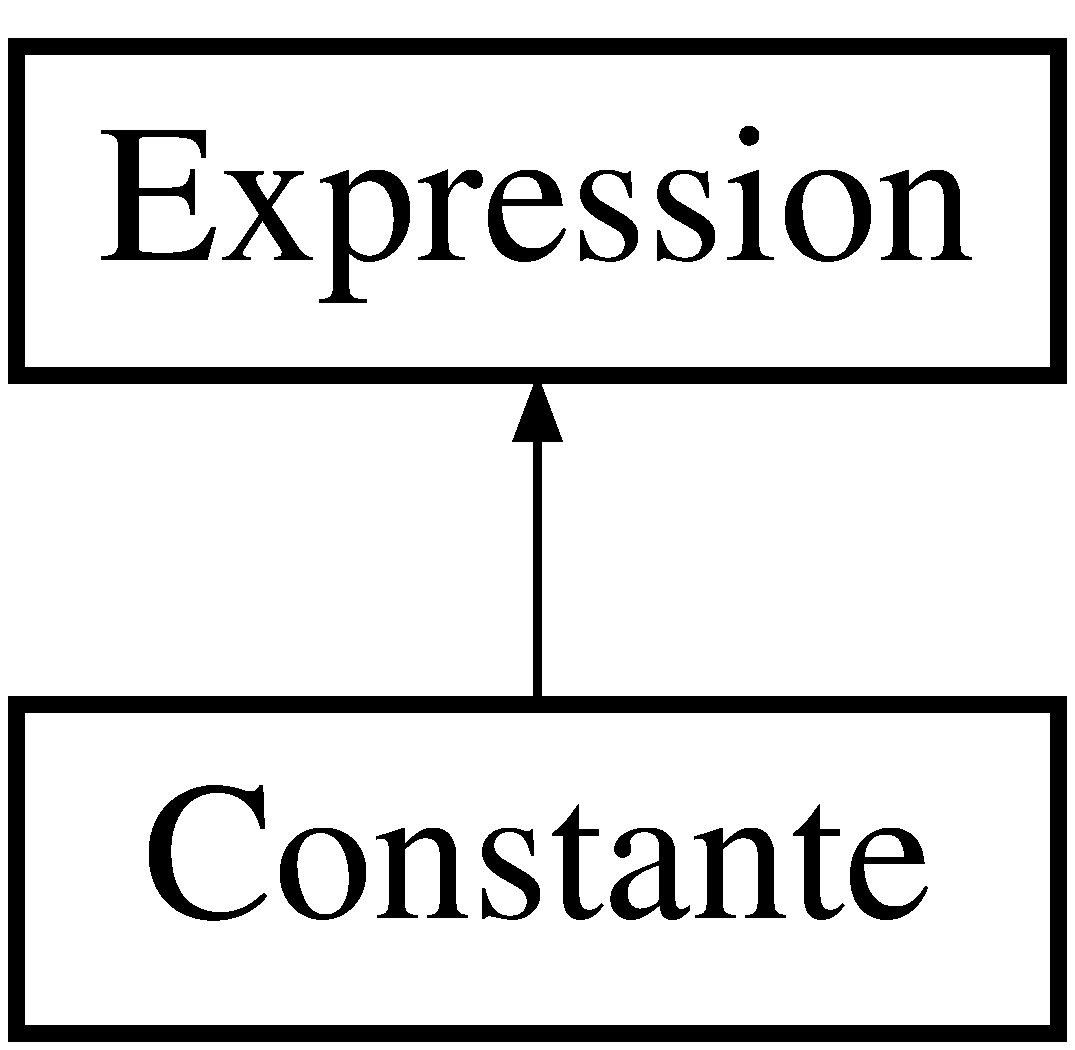
\includegraphics[height=2.000000cm]{class_constante}
\end{center}
\end{figure}
\subsection*{Public Member Functions}
\begin{DoxyCompactItemize}
\item 
\hyperlink{class_constante_ac463207a372c10cb3fe0cd999e2e2c7b}{Constante} ()
\begin{DoxyCompactList}\small\item\em Constructeur. \end{DoxyCompactList}\item 
\hyperlink{class_constante_a042ef484454ea2cbad4afbdc1693d954}{Constante} (const double=0.\+0)
\begin{DoxyCompactList}\small\item\em Constructeur. \end{DoxyCompactList}\item 
virtual \hyperlink{class_constante_a676cae1183d2db492fbe20289e96b2c5}{$\sim$\+Constante} ()
\begin{DoxyCompactList}\small\item\em Destructeur Destructeur de la classe \hyperlink{class_constante}{Constante}. \end{DoxyCompactList}\item 
virtual double \hyperlink{class_constante_aaf4b67f9a9d34aca1f689e6fbf63be75}{eval} () const 
\begin{DoxyCompactList}\small\item\em Evalue l\textquotesingle{}expression Methode qui permet d\textquotesingle{}evaluer l\textquotesingle{}expression. \end{DoxyCompactList}\item 
\hyperlink{class_expression}{Expression} $\ast$ \hyperlink{class_constante_a78c242a323b89ebc7b1ffdd817e2bd76}{deriver} (const string \&)
\begin{DoxyCompactList}\small\item\em Derive l\textquotesingle{}expression$\ast$ Methode qui permet deriver l\textquotesingle{}expression. \end{DoxyCompactList}\item 
\hyperlink{class_expression}{Expression} $\ast$ \hyperlink{class_constante_a6e034b3b42fbcfcee505303648c03d69}{simplifier} ()
\begin{DoxyCompactList}\small\item\em Simplifie l\textquotesingle{}expression Methode qui permet de simplifier l\textquotesingle{}expression. \end{DoxyCompactList}\item 
string \hyperlink{class_constante_a798db3847c1a81a68321cada88f3f43d}{afficher} () const 
\begin{DoxyCompactList}\small\item\em Affiche l\textquotesingle{}expression Methode qui permet d\textquotesingle{}afficher l\textquotesingle{}expression. \end{DoxyCompactList}\item 
\hyperlink{class_expression}{Expression} $\ast$ \hyperlink{class_constante_a3227e53212fc8381fb33c559b22b868d}{clone} () const 
\begin{DoxyCompactList}\small\item\em clone l\textquotesingle{}expression Methode qui permet de cloner l\textquotesingle{}expression \end{DoxyCompactList}\item 
string \hyperlink{class_constante_a1481b18531d5a3eefc18bd4bb1522e54}{string\+\_\+from\+\_\+double} (double val)
\end{DoxyCompactItemize}
\subsection*{Friends}
\begin{DoxyCompactItemize}
\item 
ostream \& \hyperlink{class_constante_a6a615fb5d7dc64fa67d28eb6132c767c}{operator$<$$<$} (ostream \&, const \hyperlink{class_constante}{Constante} \&)
\begin{DoxyCompactList}\small\item\em operator$<$$<$ Methode qui permet d\textquotesingle{}afficher l\textquotesingle{}expression \end{DoxyCompactList}\end{DoxyCompactItemize}
\subsection*{Additional Inherited Members}


\subsection{Detailed Description}
La classe \hyperlink{class_constante}{Constante}. 

Cette classe permet de repr�senter un expression constante qui est un valeur num�rique de type double. 

\subsection{Constructor \& Destructor Documentation}
\index{Constante@{Constante}!Constante@{Constante}}
\index{Constante@{Constante}!Constante@{Constante}}
\subsubsection[{\texorpdfstring{Constante()}{Constante()}}]{\setlength{\rightskip}{0pt plus 5cm}Constante\+::\+Constante (
\begin{DoxyParamCaption}
{}
\end{DoxyParamCaption}
)}\hypertarget{class_constante_ac463207a372c10cb3fe0cd999e2e2c7b}{}\label{class_constante_ac463207a372c10cb3fe0cd999e2e2c7b}


Constructeur. 

Constructeur de la classe \hyperlink{class_constante}{Constante} \index{Constante@{Constante}!Constante@{Constante}}
\index{Constante@{Constante}!Constante@{Constante}}
\subsubsection[{\texorpdfstring{Constante(const double=0.\+0)}{Constante(const double=0.0)}}]{\setlength{\rightskip}{0pt plus 5cm}Constante\+::\+Constante (
\begin{DoxyParamCaption}
\item[{const double}]{val = {\ttfamily 0.0}}
\end{DoxyParamCaption}
)}\hypertarget{class_constante_a042ef484454ea2cbad4afbdc1693d954}{}\label{class_constante_a042ef484454ea2cbad4afbdc1693d954}


Constructeur. 

Constructeur de la classe \hyperlink{class_constante}{Constante}


\begin{DoxyParams}{Parameters}
{\em val} & \+: le valeur \\
\hline
\end{DoxyParams}
\index{Constante@{Constante}!````~Constante@{$\sim$\+Constante}}
\index{````~Constante@{$\sim$\+Constante}!Constante@{Constante}}
\subsubsection[{\texorpdfstring{$\sim$\+Constante()}{~Constante()}}]{\setlength{\rightskip}{0pt plus 5cm}Constante\+::$\sim$\+Constante (
\begin{DoxyParamCaption}
{}
\end{DoxyParamCaption}
)\hspace{0.3cm}{\ttfamily [virtual]}}\hypertarget{class_constante_a676cae1183d2db492fbe20289e96b2c5}{}\label{class_constante_a676cae1183d2db492fbe20289e96b2c5}


Destructeur Destructeur de la classe \hyperlink{class_constante}{Constante}. 



\subsection{Member Function Documentation}
\index{Constante@{Constante}!afficher@{afficher}}
\index{afficher@{afficher}!Constante@{Constante}}
\subsubsection[{\texorpdfstring{afficher() const }{afficher() const }}]{\setlength{\rightskip}{0pt plus 5cm}string Constante\+::afficher (
\begin{DoxyParamCaption}
{}
\end{DoxyParamCaption}
) const\hspace{0.3cm}{\ttfamily [virtual]}}\hypertarget{class_constante_a798db3847c1a81a68321cada88f3f43d}{}\label{class_constante_a798db3847c1a81a68321cada88f3f43d}


Affiche l\textquotesingle{}expression Methode qui permet d\textquotesingle{}afficher l\textquotesingle{}expression. 

\begin{DoxyReturn}{Returns}
Le string d\textquotesingle{}expression 
\end{DoxyReturn}


Reimplemented from \hyperlink{class_expression_a953c7de0302331023987a2fff895cb85}{Expression}.

\index{Constante@{Constante}!clone@{clone}}
\index{clone@{clone}!Constante@{Constante}}
\subsubsection[{\texorpdfstring{clone() const }{clone() const }}]{\setlength{\rightskip}{0pt plus 5cm}{\bf Expression} $\ast$ Constante\+::clone (
\begin{DoxyParamCaption}
{}
\end{DoxyParamCaption}
) const\hspace{0.3cm}{\ttfamily [virtual]}}\hypertarget{class_constante_a3227e53212fc8381fb33c559b22b868d}{}\label{class_constante_a3227e53212fc8381fb33c559b22b868d}


clone l\textquotesingle{}expression Methode qui permet de cloner l\textquotesingle{}expression 

\begin{DoxyReturn}{Returns}
L\textquotesingle{}expression clon� 
\end{DoxyReturn}


Implements \hyperlink{class_expression_ac9fcea09ddd3a650a92c3606118abfb6}{Expression}.

\index{Constante@{Constante}!deriver@{deriver}}
\index{deriver@{deriver}!Constante@{Constante}}
\subsubsection[{\texorpdfstring{deriver(const string \&)}{deriver(const string &)}}]{\setlength{\rightskip}{0pt plus 5cm}{\bf Expression} $\ast$ Constante\+::deriver (
\begin{DoxyParamCaption}
\item[{const string \&}]{var}
\end{DoxyParamCaption}
)\hspace{0.3cm}{\ttfamily [virtual]}}\hypertarget{class_constante_a78c242a323b89ebc7b1ffdd817e2bd76}{}\label{class_constante_a78c242a323b89ebc7b1ffdd817e2bd76}


Derive l\textquotesingle{}expression$\ast$ Methode qui permet deriver l\textquotesingle{}expression. 

\begin{DoxyReturn}{Returns}
L\textquotesingle{}expression deriv� 
\end{DoxyReturn}


Implements \hyperlink{class_expression_a0a2a2cf2cdb1e8ca556ad59832784193}{Expression}.

\index{Constante@{Constante}!eval@{eval}}
\index{eval@{eval}!Constante@{Constante}}
\subsubsection[{\texorpdfstring{eval() const }{eval() const }}]{\setlength{\rightskip}{0pt plus 5cm}double Constante\+::eval (
\begin{DoxyParamCaption}
{}
\end{DoxyParamCaption}
) const\hspace{0.3cm}{\ttfamily [virtual]}}\hypertarget{class_constante_aaf4b67f9a9d34aca1f689e6fbf63be75}{}\label{class_constante_aaf4b67f9a9d34aca1f689e6fbf63be75}


Evalue l\textquotesingle{}expression Methode qui permet d\textquotesingle{}evaluer l\textquotesingle{}expression. 

\begin{DoxyReturn}{Returns}
Le valeur d\textquotesingle{}expression 
\end{DoxyReturn}


Implements \hyperlink{class_expression_a5481c36265e11eff513df87bbc5a1d33}{Expression}.

\index{Constante@{Constante}!simplifier@{simplifier}}
\index{simplifier@{simplifier}!Constante@{Constante}}
\subsubsection[{\texorpdfstring{simplifier()}{simplifier()}}]{\setlength{\rightskip}{0pt plus 5cm}{\bf Expression} $\ast$ Constante\+::simplifier (
\begin{DoxyParamCaption}
{}
\end{DoxyParamCaption}
)\hspace{0.3cm}{\ttfamily [virtual]}}\hypertarget{class_constante_a6e034b3b42fbcfcee505303648c03d69}{}\label{class_constante_a6e034b3b42fbcfcee505303648c03d69}


Simplifie l\textquotesingle{}expression Methode qui permet de simplifier l\textquotesingle{}expression. 

\begin{DoxyReturn}{Returns}
L\textquotesingle{}expression simplifi� 
\end{DoxyReturn}


Implements \hyperlink{class_expression_a319d06d43ead325c835181419061ae0b}{Expression}.

\index{Constante@{Constante}!string\+\_\+from\+\_\+double@{string\+\_\+from\+\_\+double}}
\index{string\+\_\+from\+\_\+double@{string\+\_\+from\+\_\+double}!Constante@{Constante}}
\subsubsection[{\texorpdfstring{string\+\_\+from\+\_\+double(double val)}{string_from_double(double val)}}]{\setlength{\rightskip}{0pt plus 5cm}string Constante\+::string\+\_\+from\+\_\+double (
\begin{DoxyParamCaption}
\item[{double}]{val}
\end{DoxyParamCaption}
)\hspace{0.3cm}{\ttfamily [inline]}}\hypertarget{class_constante_a1481b18531d5a3eefc18bd4bb1522e54}{}\label{class_constante_a1481b18531d5a3eefc18bd4bb1522e54}


\subsection{Friends And Related Function Documentation}
\index{Constante@{Constante}!operator$<$$<$@{operator$<$$<$}}
\index{operator$<$$<$@{operator$<$$<$}!Constante@{Constante}}
\subsubsection[{\texorpdfstring{operator$<$$<$}{operator<<}}]{\setlength{\rightskip}{0pt plus 5cm}ostream\& operator$<$$<$ (
\begin{DoxyParamCaption}
\item[{ostream \&}]{os, }
\item[{const {\bf Constante} \&}]{constante}
\end{DoxyParamCaption}
)\hspace{0.3cm}{\ttfamily [friend]}}\hypertarget{class_constante_a6a615fb5d7dc64fa67d28eb6132c767c}{}\label{class_constante_a6a615fb5d7dc64fa67d28eb6132c767c}


operator$<$$<$ Methode qui permet d\textquotesingle{}afficher l\textquotesingle{}expression 



The documentation for this class was generated from the following files\+:\begin{DoxyCompactItemize}
\item 
include/\hyperlink{constante_8h}{constante.\+h}\item 
src/\hyperlink{constante_8cpp}{constante.\+cpp}\end{DoxyCompactItemize}

\hypertarget{class_cos}{}\section{Cos Class Reference}
\label{class_cos}\index{Cos@{Cos}}


La classe \hyperlink{class_cos}{Cos}.  




{\ttfamily \#include $<$unaire.\+h$>$}

Inheritance diagram for Cos\+:\begin{figure}[H]
\begin{center}
\leavevmode
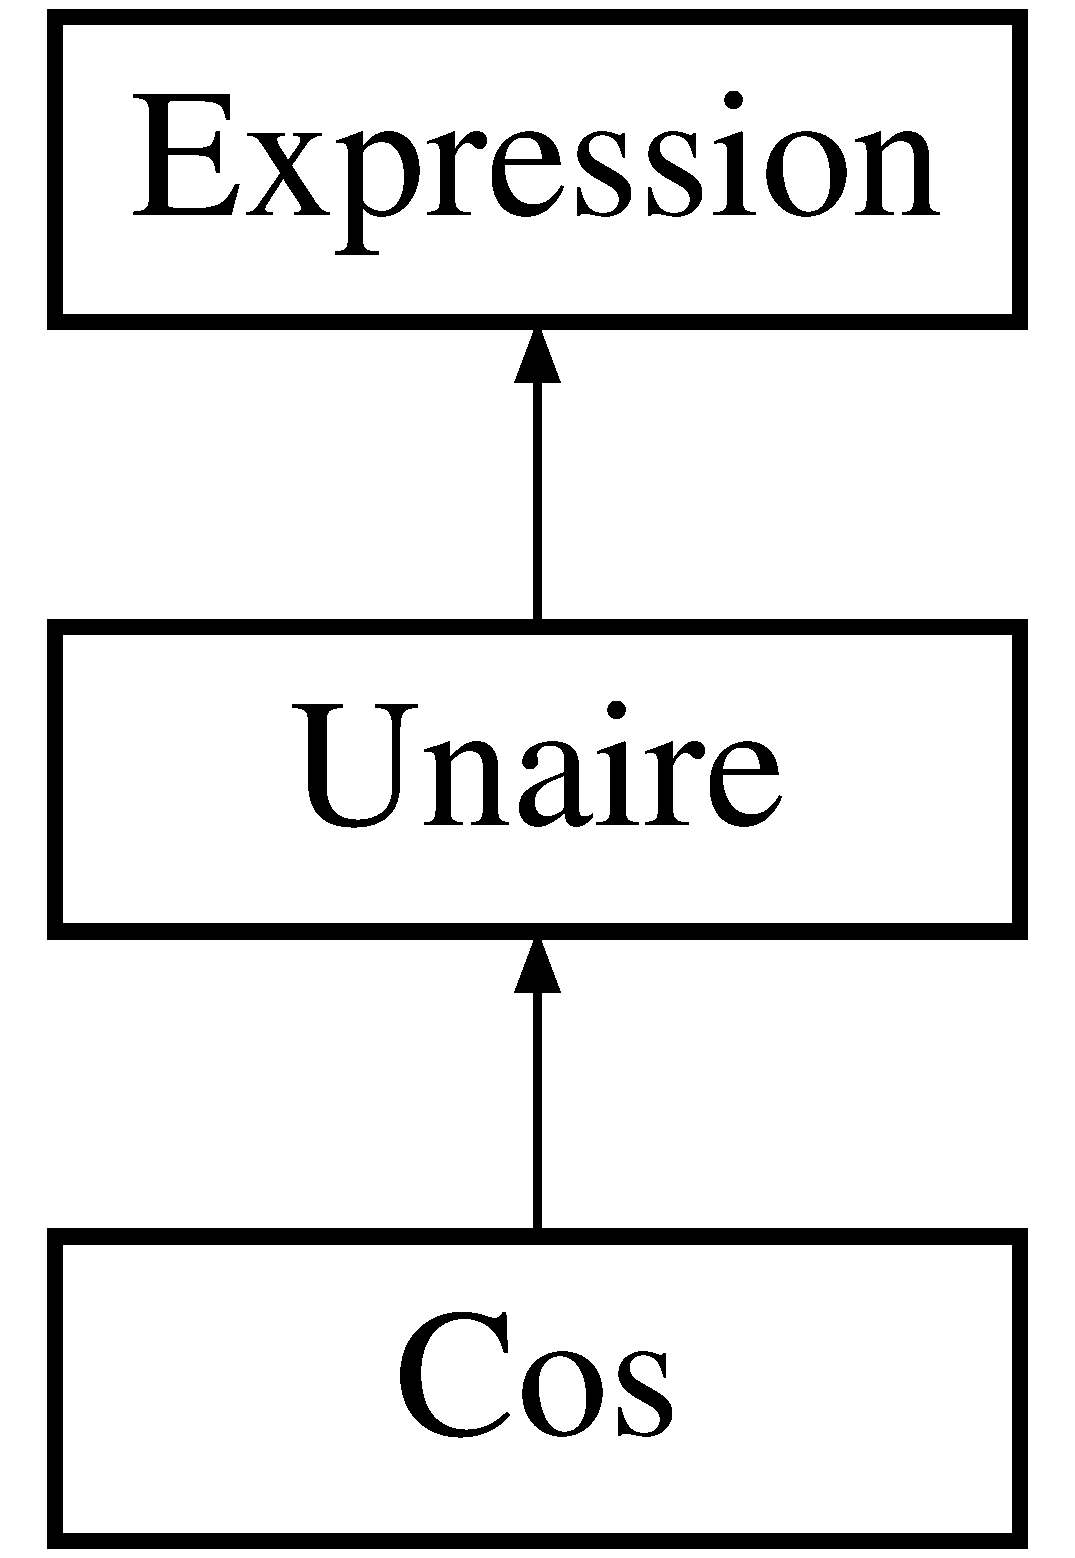
\includegraphics[height=3.000000cm]{class_cos}
\end{center}
\end{figure}
\subsection*{Public Member Functions}
\begin{DoxyCompactItemize}
\item 
\hyperlink{class_cos_afcabb31f1ff7871afba44a04b78e24c1}{Cos} ()
\begin{DoxyCompactList}\small\item\em Constructeur. \end{DoxyCompactList}\item 
\hyperlink{class_cos_abe655cf38ff64ebec69829a38bdb6736}{Cos} (\hyperlink{class_expression}{Expression} $\ast$, const string \&name=\char`\"{}cos\char`\"{})
\begin{DoxyCompactList}\small\item\em Constructeur. \end{DoxyCompactList}\item 
virtual \hyperlink{class_cos_ae17e500c0efd3657db2c9da979c1f2c5}{$\sim$\+Cos} ()
\begin{DoxyCompactList}\small\item\em Destructeur Destructeur de la classe \hyperlink{class_affectation}{Affectation}. \end{DoxyCompactList}\item 
double \hyperlink{class_cos_a601f93938da00a524c3cce3a9bcc6c7d}{eval} () const 
\begin{DoxyCompactList}\small\item\em Evalue l\textquotesingle{}expression Methode qui permet d\textquotesingle{}evaluer l\textquotesingle{}expression. \end{DoxyCompactList}\item 
\hyperlink{class_expression}{Expression} $\ast$ \hyperlink{class_cos_a23bcff67edb0140231ea0b00f68f9a3a}{deriver} (const string \&)
\begin{DoxyCompactList}\small\item\em Derive l\textquotesingle{}expression$\ast$ Methode qui permet deriver l\textquotesingle{}expression. \end{DoxyCompactList}\item 
\hyperlink{class_expression}{Expression} $\ast$ \hyperlink{class_cos_ae22a7bd0a5caf0cab864f80e954ecd34}{simplifier} ()
\begin{DoxyCompactList}\small\item\em Simplifie l\textquotesingle{}expression Methode qui permet de simplifier l\textquotesingle{}expression. \end{DoxyCompactList}\item 
\hyperlink{class_expression}{Expression} $\ast$ \hyperlink{class_cos_a1c4eb6ff08383ac08e7b511aa9d50fb2}{clone} () const 
\begin{DoxyCompactList}\small\item\em clone l\textquotesingle{}expression Methode qui permet de cloner l\textquotesingle{}expression \end{DoxyCompactList}\end{DoxyCompactItemize}
\subsection*{Protected Attributes}
\begin{DoxyCompactItemize}
\item 
double \hyperlink{class_cos_a2e1acb03226446c800db4a2a3e3433b2}{val}
\end{DoxyCompactItemize}
\subsection*{Additional Inherited Members}


\subsection{Detailed Description}
La classe \hyperlink{class_cos}{Cos}. 

Cette classe repr�sente le \hyperlink{class_cos}{Cos}. 

\subsection{Constructor \& Destructor Documentation}
\index{Cos@{Cos}!Cos@{Cos}}
\index{Cos@{Cos}!Cos@{Cos}}
\subsubsection[{\texorpdfstring{Cos()}{Cos()}}]{\setlength{\rightskip}{0pt plus 5cm}Cos\+::\+Cos (
\begin{DoxyParamCaption}
{}
\end{DoxyParamCaption}
)}\hypertarget{class_cos_afcabb31f1ff7871afba44a04b78e24c1}{}\label{class_cos_afcabb31f1ff7871afba44a04b78e24c1}


Constructeur. 

Constructeur de la classe \hyperlink{class_cos}{Cos} \index{Cos@{Cos}!Cos@{Cos}}
\index{Cos@{Cos}!Cos@{Cos}}
\subsubsection[{\texorpdfstring{Cos(\+Expression $\ast$, const string \&name=""cos"")}{Cos(Expression *, const string &name="cos")}}]{\setlength{\rightskip}{0pt plus 5cm}Cos\+::\+Cos (
\begin{DoxyParamCaption}
\item[{{\bf Expression} $\ast$}]{exp, }
\item[{const string \&}]{name = {\ttfamily \char`\"{}cos\char`\"{}}}
\end{DoxyParamCaption}
)}\hypertarget{class_cos_abe655cf38ff64ebec69829a38bdb6736}{}\label{class_cos_abe655cf38ff64ebec69829a38bdb6736}


Constructeur. 

Constructeur de la classe \hyperlink{class_cos}{Cos}


\begin{DoxyParams}{Parameters}
{\em exp} & \+: l\textquotesingle{}expression \\
\hline
{\em nom} & \+: le nom \\
\hline
\end{DoxyParams}
\index{Cos@{Cos}!````~Cos@{$\sim$\+Cos}}
\index{````~Cos@{$\sim$\+Cos}!Cos@{Cos}}
\subsubsection[{\texorpdfstring{$\sim$\+Cos()}{~Cos()}}]{\setlength{\rightskip}{0pt plus 5cm}Cos\+::$\sim$\+Cos (
\begin{DoxyParamCaption}
{}
\end{DoxyParamCaption}
)\hspace{0.3cm}{\ttfamily [virtual]}}\hypertarget{class_cos_ae17e500c0efd3657db2c9da979c1f2c5}{}\label{class_cos_ae17e500c0efd3657db2c9da979c1f2c5}


Destructeur Destructeur de la classe \hyperlink{class_affectation}{Affectation}. 



\subsection{Member Function Documentation}
\index{Cos@{Cos}!clone@{clone}}
\index{clone@{clone}!Cos@{Cos}}
\subsubsection[{\texorpdfstring{clone() const }{clone() const }}]{\setlength{\rightskip}{0pt plus 5cm}{\bf Expression} $\ast$ Cos\+::clone (
\begin{DoxyParamCaption}
{}
\end{DoxyParamCaption}
) const\hspace{0.3cm}{\ttfamily [virtual]}}\hypertarget{class_cos_a1c4eb6ff08383ac08e7b511aa9d50fb2}{}\label{class_cos_a1c4eb6ff08383ac08e7b511aa9d50fb2}


clone l\textquotesingle{}expression Methode qui permet de cloner l\textquotesingle{}expression 

\begin{DoxyReturn}{Returns}
L\textquotesingle{}expression clon� 
\end{DoxyReturn}


Implements \hyperlink{class_expression_ac9fcea09ddd3a650a92c3606118abfb6}{Expression}.

\index{Cos@{Cos}!deriver@{deriver}}
\index{deriver@{deriver}!Cos@{Cos}}
\subsubsection[{\texorpdfstring{deriver(const string \&)}{deriver(const string &)}}]{\setlength{\rightskip}{0pt plus 5cm}{\bf Expression} $\ast$ Cos\+::deriver (
\begin{DoxyParamCaption}
\item[{const string \&}]{var}
\end{DoxyParamCaption}
)\hspace{0.3cm}{\ttfamily [virtual]}}\hypertarget{class_cos_a23bcff67edb0140231ea0b00f68f9a3a}{}\label{class_cos_a23bcff67edb0140231ea0b00f68f9a3a}


Derive l\textquotesingle{}expression$\ast$ Methode qui permet deriver l\textquotesingle{}expression. 

\begin{DoxyReturn}{Returns}
L\textquotesingle{}expression deriv� 
\end{DoxyReturn}


Implements \hyperlink{class_expression_a0a2a2cf2cdb1e8ca556ad59832784193}{Expression}.

\index{Cos@{Cos}!eval@{eval}}
\index{eval@{eval}!Cos@{Cos}}
\subsubsection[{\texorpdfstring{eval() const }{eval() const }}]{\setlength{\rightskip}{0pt plus 5cm}double Cos\+::eval (
\begin{DoxyParamCaption}
{}
\end{DoxyParamCaption}
) const\hspace{0.3cm}{\ttfamily [virtual]}}\hypertarget{class_cos_a601f93938da00a524c3cce3a9bcc6c7d}{}\label{class_cos_a601f93938da00a524c3cce3a9bcc6c7d}


Evalue l\textquotesingle{}expression Methode qui permet d\textquotesingle{}evaluer l\textquotesingle{}expression. 

\begin{DoxyReturn}{Returns}
Le valeur d\textquotesingle{}expression 
\end{DoxyReturn}


Implements \hyperlink{class_expression_a5481c36265e11eff513df87bbc5a1d33}{Expression}.

\index{Cos@{Cos}!simplifier@{simplifier}}
\index{simplifier@{simplifier}!Cos@{Cos}}
\subsubsection[{\texorpdfstring{simplifier()}{simplifier()}}]{\setlength{\rightskip}{0pt plus 5cm}{\bf Expression} $\ast$ Cos\+::simplifier (
\begin{DoxyParamCaption}
{}
\end{DoxyParamCaption}
)\hspace{0.3cm}{\ttfamily [virtual]}}\hypertarget{class_cos_ae22a7bd0a5caf0cab864f80e954ecd34}{}\label{class_cos_ae22a7bd0a5caf0cab864f80e954ecd34}


Simplifie l\textquotesingle{}expression Methode qui permet de simplifier l\textquotesingle{}expression. 

\begin{DoxyReturn}{Returns}
L\textquotesingle{}expression simplifi� 
\end{DoxyReturn}


Implements \hyperlink{class_expression_a319d06d43ead325c835181419061ae0b}{Expression}.



\subsection{Member Data Documentation}
\index{Cos@{Cos}!val@{val}}
\index{val@{val}!Cos@{Cos}}
\subsubsection[{\texorpdfstring{val}{val}}]{\setlength{\rightskip}{0pt plus 5cm}double Cos\+::val\hspace{0.3cm}{\ttfamily [protected]}}\hypertarget{class_cos_a2e1acb03226446c800db4a2a3e3433b2}{}\label{class_cos_a2e1acb03226446c800db4a2a3e3433b2}


The documentation for this class was generated from the following files\+:\begin{DoxyCompactItemize}
\item 
include/\hyperlink{unaire_8h}{unaire.\+h}\item 
src/\hyperlink{unaire_8cpp}{unaire.\+cpp}\end{DoxyCompactItemize}

\hypertarget{class_difference}{}\section{Difference Class Reference}
\label{class_difference}\index{Difference@{Difference}}


La classe \hyperlink{class_difference}{Difference}.  




{\ttfamily \#include $<$binaire.\+h$>$}

Inheritance diagram for Difference\+:\begin{figure}[H]
\begin{center}
\leavevmode
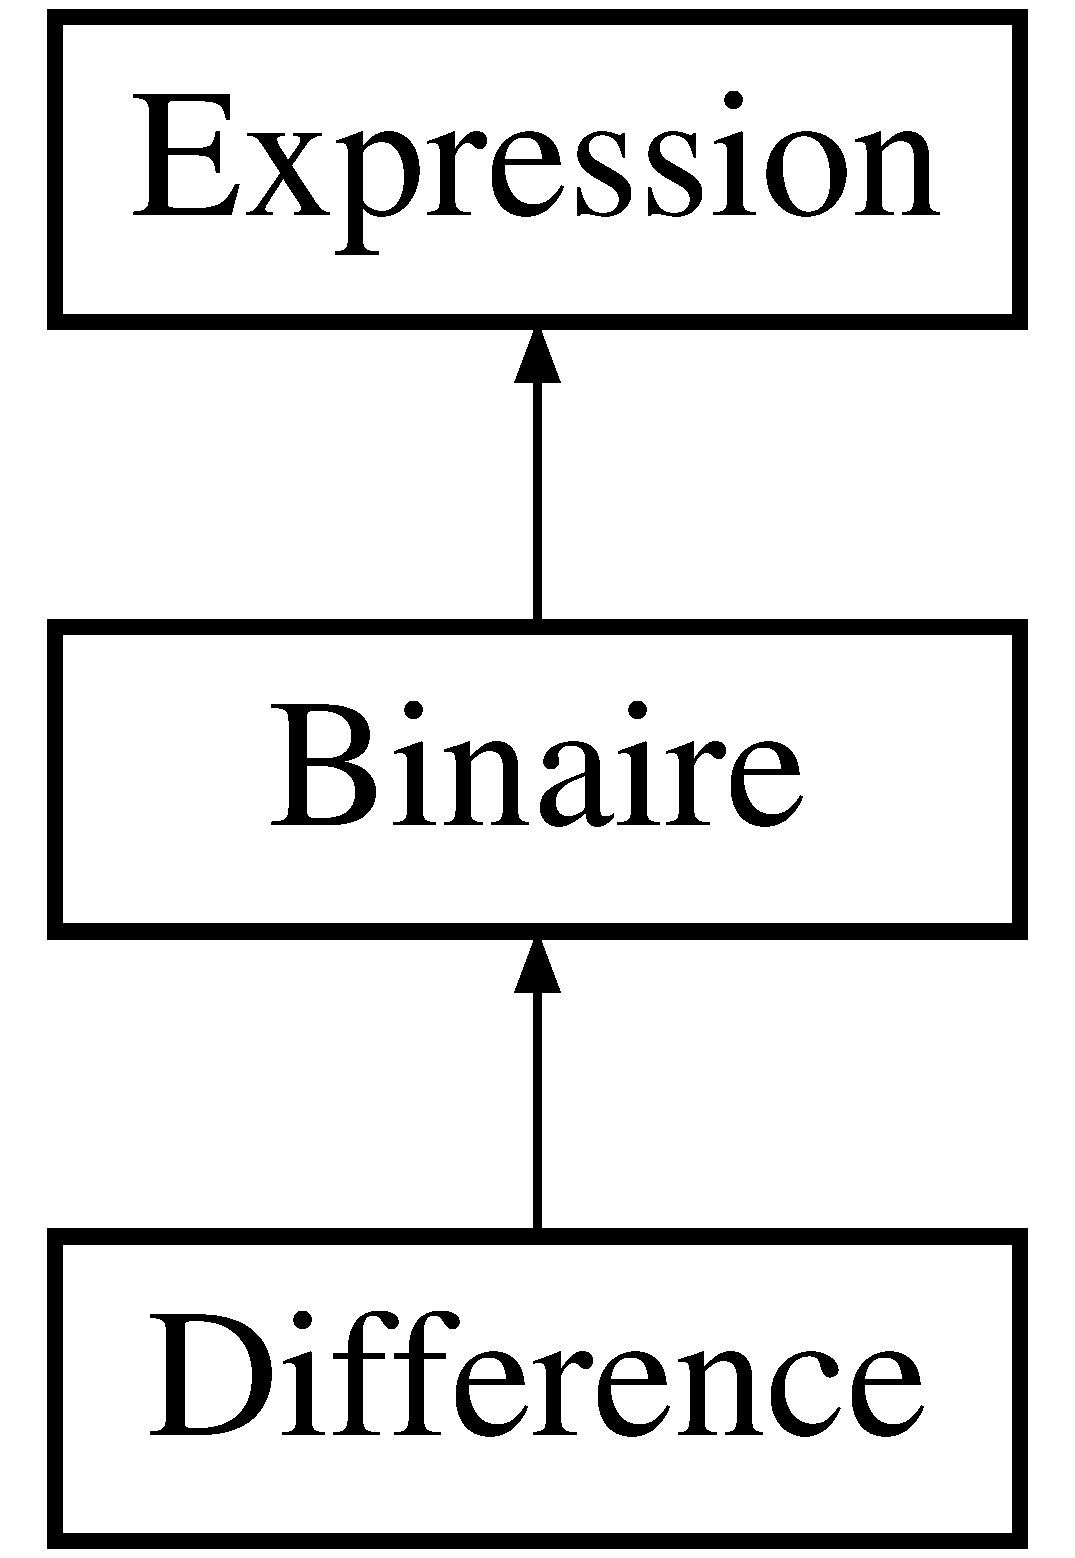
\includegraphics[height=3.000000cm]{class_difference}
\end{center}
\end{figure}
\subsection*{Public Member Functions}
\begin{DoxyCompactItemize}
\item 
\hyperlink{class_difference_a41aaa289ccbc98fb583d2c4fb95dc371}{Difference} ()
\begin{DoxyCompactList}\small\item\em Constructeur. \end{DoxyCompactList}\item 
virtual \hyperlink{class_difference_a7cb04c0ecbc557cc93d05fbabd3b25ce}{$\sim$\+Difference} ()
\begin{DoxyCompactList}\small\item\em Destructeur Destructeur de la classe \hyperlink{class_difference}{Difference}. \end{DoxyCompactList}\item 
double \hyperlink{class_difference_a0da9cd3169bea5ca70af3f4aed9a55a8}{eval} () const 
\begin{DoxyCompactList}\small\item\em Evalue l\textquotesingle{}expression Methode qui permet d\textquotesingle{}evaluer l\textquotesingle{}expression. \end{DoxyCompactList}\item 
\hyperlink{class_expression}{Expression} $\ast$ \hyperlink{class_difference_af9118a276538e992bff5dfcae3d3b25f}{deriver} (const string \&)
\begin{DoxyCompactList}\small\item\em Derive l\textquotesingle{}expression$\ast$ Methode qui permet deriver l\textquotesingle{}expression. \end{DoxyCompactList}\item 
\hyperlink{class_expression}{Expression} $\ast$ \hyperlink{class_difference_a1ea49952e410f10cc4907e80ac2597d4}{simplifier} ()
\begin{DoxyCompactList}\small\item\em Simplifie l\textquotesingle{}expression Methode qui permet de simplifier l\textquotesingle{}expression. \end{DoxyCompactList}\item 
\hyperlink{class_expression}{Expression} $\ast$ \hyperlink{class_difference_a3bd254abd06c7ed2b6946c7682bec584}{clone} () const 
\begin{DoxyCompactList}\small\item\em clone l\textquotesingle{}expression Methode qui permet de cloner l\textquotesingle{}expression \end{DoxyCompactList}\item 
string \hyperlink{class_difference_af06c097f3901551229b8a7b73bccb94b}{afficher} () const 
\begin{DoxyCompactList}\small\item\em Affiche l\textquotesingle{}expression Methode qui permet d\textquotesingle{}afficher l\textquotesingle{}expression. \end{DoxyCompactList}\item 
\hyperlink{class_difference_ad8c652e7378cb91ce262407094940cc3}{Difference} (\hyperlink{class_expression}{Expression} $\ast$, \hyperlink{class_expression}{Expression} $\ast$, const string \&name=\char`\"{}-\/\char`\"{})
\begin{DoxyCompactList}\small\item\em Constructeur. \end{DoxyCompactList}\end{DoxyCompactItemize}
\subsection*{Friends}
\begin{DoxyCompactItemize}
\item 
ostream \& \hyperlink{class_difference_a594e02d1e0c9961e67025ebf975bc079}{operator$<$$<$} (ostream \&, const \hyperlink{class_difference}{Difference} \&)
\begin{DoxyCompactList}\small\item\em operator$<$$<$ Methode qui permet d\textquotesingle{}afficher l\textquotesingle{}expression \end{DoxyCompactList}\end{DoxyCompactItemize}
\subsection*{Additional Inherited Members}


\subsection{Detailed Description}
La classe \hyperlink{class_difference}{Difference}. 

Cette classe repr�sente le soustraction 

\subsection{Constructor \& Destructor Documentation}
\index{Difference@{Difference}!Difference@{Difference}}
\index{Difference@{Difference}!Difference@{Difference}}
\subsubsection[{\texorpdfstring{Difference()}{Difference()}}]{\setlength{\rightskip}{0pt plus 5cm}Difference\+::\+Difference (
\begin{DoxyParamCaption}
{}
\end{DoxyParamCaption}
)}\hypertarget{class_difference_a41aaa289ccbc98fb583d2c4fb95dc371}{}\label{class_difference_a41aaa289ccbc98fb583d2c4fb95dc371}


Constructeur. 

Constructeur de la classe \hyperlink{class_difference}{Difference} \index{Difference@{Difference}!````~Difference@{$\sim$\+Difference}}
\index{````~Difference@{$\sim$\+Difference}!Difference@{Difference}}
\subsubsection[{\texorpdfstring{$\sim$\+Difference()}{~Difference()}}]{\setlength{\rightskip}{0pt plus 5cm}Difference\+::$\sim$\+Difference (
\begin{DoxyParamCaption}
{}
\end{DoxyParamCaption}
)\hspace{0.3cm}{\ttfamily [virtual]}}\hypertarget{class_difference_a7cb04c0ecbc557cc93d05fbabd3b25ce}{}\label{class_difference_a7cb04c0ecbc557cc93d05fbabd3b25ce}


Destructeur Destructeur de la classe \hyperlink{class_difference}{Difference}. 

\index{Difference@{Difference}!Difference@{Difference}}
\index{Difference@{Difference}!Difference@{Difference}}
\subsubsection[{\texorpdfstring{Difference(\+Expression $\ast$, Expression $\ast$, const string \&name=""-\/"")}{Difference(Expression *, Expression *, const string &name="-")}}]{\setlength{\rightskip}{0pt plus 5cm}Difference\+::\+Difference (
\begin{DoxyParamCaption}
\item[{{\bf Expression} $\ast$}]{exp1, }
\item[{{\bf Expression} $\ast$}]{exp2, }
\item[{const string \&}]{name = {\ttfamily \char`\"{}-\/\char`\"{}}}
\end{DoxyParamCaption}
)}\hypertarget{class_difference_ad8c652e7378cb91ce262407094940cc3}{}\label{class_difference_ad8c652e7378cb91ce262407094940cc3}


Constructeur. 

Constructeur de la classe \hyperlink{class_difference}{Difference}


\begin{DoxyParams}{Parameters}
{\em exp1} & \+: op�rande gauche \\
\hline
{\em exp2} & \+: op�rande droite \\
\hline
{\em nom} & \+: nom d\textquotesingle{}expression \\
\hline
\end{DoxyParams}


\subsection{Member Function Documentation}
\index{Difference@{Difference}!afficher@{afficher}}
\index{afficher@{afficher}!Difference@{Difference}}
\subsubsection[{\texorpdfstring{afficher() const }{afficher() const }}]{\setlength{\rightskip}{0pt plus 5cm}string Difference\+::afficher (
\begin{DoxyParamCaption}
{}
\end{DoxyParamCaption}
) const\hspace{0.3cm}{\ttfamily [virtual]}}\hypertarget{class_difference_af06c097f3901551229b8a7b73bccb94b}{}\label{class_difference_af06c097f3901551229b8a7b73bccb94b}


Affiche l\textquotesingle{}expression Methode qui permet d\textquotesingle{}afficher l\textquotesingle{}expression. 

\begin{DoxyReturn}{Returns}
Le string d\textquotesingle{}expression 
\end{DoxyReturn}


Reimplemented from \hyperlink{class_expression_a953c7de0302331023987a2fff895cb85}{Expression}.

\index{Difference@{Difference}!clone@{clone}}
\index{clone@{clone}!Difference@{Difference}}
\subsubsection[{\texorpdfstring{clone() const }{clone() const }}]{\setlength{\rightskip}{0pt plus 5cm}{\bf Expression} $\ast$ Difference\+::clone (
\begin{DoxyParamCaption}
{}
\end{DoxyParamCaption}
) const\hspace{0.3cm}{\ttfamily [virtual]}}\hypertarget{class_difference_a3bd254abd06c7ed2b6946c7682bec584}{}\label{class_difference_a3bd254abd06c7ed2b6946c7682bec584}


clone l\textquotesingle{}expression Methode qui permet de cloner l\textquotesingle{}expression 

\begin{DoxyReturn}{Returns}
L\textquotesingle{}expression clon� 
\end{DoxyReturn}


Implements \hyperlink{class_expression_ac9fcea09ddd3a650a92c3606118abfb6}{Expression}.

\index{Difference@{Difference}!deriver@{deriver}}
\index{deriver@{deriver}!Difference@{Difference}}
\subsubsection[{\texorpdfstring{deriver(const string \&)}{deriver(const string &)}}]{\setlength{\rightskip}{0pt plus 5cm}{\bf Expression} $\ast$ Difference\+::deriver (
\begin{DoxyParamCaption}
\item[{const string \&}]{var}
\end{DoxyParamCaption}
)\hspace{0.3cm}{\ttfamily [virtual]}}\hypertarget{class_difference_af9118a276538e992bff5dfcae3d3b25f}{}\label{class_difference_af9118a276538e992bff5dfcae3d3b25f}


Derive l\textquotesingle{}expression$\ast$ Methode qui permet deriver l\textquotesingle{}expression. 

\begin{DoxyReturn}{Returns}
L\textquotesingle{}expression deriv� 
\end{DoxyReturn}


Implements \hyperlink{class_expression_a0a2a2cf2cdb1e8ca556ad59832784193}{Expression}.

\index{Difference@{Difference}!eval@{eval}}
\index{eval@{eval}!Difference@{Difference}}
\subsubsection[{\texorpdfstring{eval() const }{eval() const }}]{\setlength{\rightskip}{0pt plus 5cm}double Difference\+::eval (
\begin{DoxyParamCaption}
{}
\end{DoxyParamCaption}
) const\hspace{0.3cm}{\ttfamily [virtual]}}\hypertarget{class_difference_a0da9cd3169bea5ca70af3f4aed9a55a8}{}\label{class_difference_a0da9cd3169bea5ca70af3f4aed9a55a8}


Evalue l\textquotesingle{}expression Methode qui permet d\textquotesingle{}evaluer l\textquotesingle{}expression. 

\begin{DoxyReturn}{Returns}
Le valeur d\textquotesingle{}expression 
\end{DoxyReturn}


Implements \hyperlink{class_expression_a5481c36265e11eff513df87bbc5a1d33}{Expression}.

\index{Difference@{Difference}!simplifier@{simplifier}}
\index{simplifier@{simplifier}!Difference@{Difference}}
\subsubsection[{\texorpdfstring{simplifier()}{simplifier()}}]{\setlength{\rightskip}{0pt plus 5cm}{\bf Expression} $\ast$ Difference\+::simplifier (
\begin{DoxyParamCaption}
{}
\end{DoxyParamCaption}
)\hspace{0.3cm}{\ttfamily [virtual]}}\hypertarget{class_difference_a1ea49952e410f10cc4907e80ac2597d4}{}\label{class_difference_a1ea49952e410f10cc4907e80ac2597d4}


Simplifie l\textquotesingle{}expression Methode qui permet de simplifier l\textquotesingle{}expression. 

\begin{DoxyReturn}{Returns}
L\textquotesingle{}expression simplifi� 
\end{DoxyReturn}


Implements \hyperlink{class_expression_a319d06d43ead325c835181419061ae0b}{Expression}.



\subsection{Friends And Related Function Documentation}
\index{Difference@{Difference}!operator$<$$<$@{operator$<$$<$}}
\index{operator$<$$<$@{operator$<$$<$}!Difference@{Difference}}
\subsubsection[{\texorpdfstring{operator$<$$<$}{operator<<}}]{\setlength{\rightskip}{0pt plus 5cm}ostream\& operator$<$$<$ (
\begin{DoxyParamCaption}
\item[{ostream \&}]{os, }
\item[{const {\bf Difference} \&}]{a}
\end{DoxyParamCaption}
)\hspace{0.3cm}{\ttfamily [friend]}}\hypertarget{class_difference_a594e02d1e0c9961e67025ebf975bc079}{}\label{class_difference_a594e02d1e0c9961e67025ebf975bc079}


operator$<$$<$ Methode qui permet d\textquotesingle{}afficher l\textquotesingle{}expression 



The documentation for this class was generated from the following files\+:\begin{DoxyCompactItemize}
\item 
include/\hyperlink{binaire_8h}{binaire.\+h}\item 
src/\hyperlink{binaire_8cpp}{binaire.\+cpp}\end{DoxyCompactItemize}

\hypertarget{class_division}{}\section{Division Class Reference}
\label{class_division}\index{Division@{Division}}


La classe \hyperlink{class_division}{Division}.  




{\ttfamily \#include $<$binaire.\+h$>$}

Inheritance diagram for Division\+:\begin{figure}[H]
\begin{center}
\leavevmode
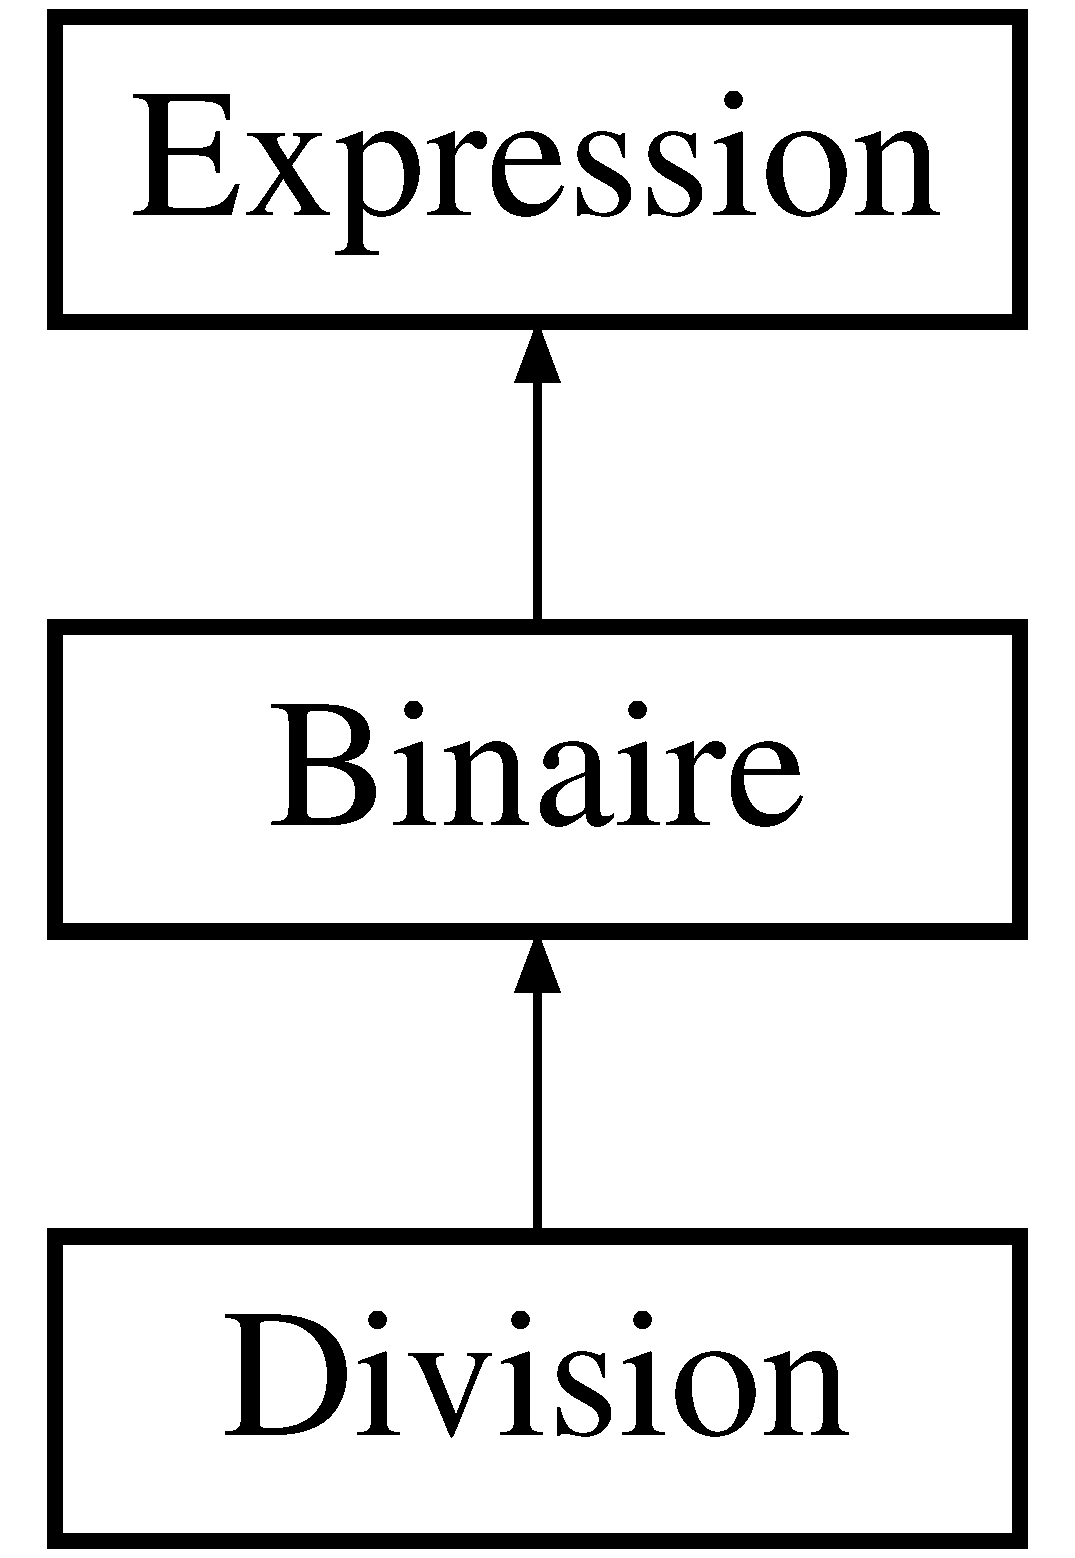
\includegraphics[height=3.000000cm]{class_division}
\end{center}
\end{figure}
\subsection*{Public Member Functions}
\begin{DoxyCompactItemize}
\item 
\hyperlink{class_division_a1cae0ab3b18df50d9986d2b879b7f464}{Division} ()
\begin{DoxyCompactList}\small\item\em Constructeur. \end{DoxyCompactList}\item 
virtual \hyperlink{class_division_a7f08073a7e2e201182af12610cd5e3eb}{$\sim$\+Division} ()
\begin{DoxyCompactList}\small\item\em Destructeur Destructeur de la classe \hyperlink{class_division}{Division}. \end{DoxyCompactList}\item 
double \hyperlink{class_division_a58dbaea10d63a27367155141cb9db323}{eval} () const 
\begin{DoxyCompactList}\small\item\em Evalue l\textquotesingle{}expression Methode qui permet d\textquotesingle{}evaluer l\textquotesingle{}expression. \end{DoxyCompactList}\item 
\hyperlink{class_expression}{Expression} $\ast$ \hyperlink{class_division_a810f31960659e2a95ddfe4f49e08cb99}{clone} () const 
\begin{DoxyCompactList}\small\item\em clone l\textquotesingle{}expression Methode qui permet de cloner l\textquotesingle{}expression \end{DoxyCompactList}\item 
string \hyperlink{class_division_af4b4b119ddfb23fd84244ac4eb6b5388}{afficher} () const 
\begin{DoxyCompactList}\small\item\em Affiche l\textquotesingle{}expression Methode qui permet d\textquotesingle{}afficher l\textquotesingle{}expression. \end{DoxyCompactList}\item 
\hyperlink{class_expression}{Expression} $\ast$ \hyperlink{class_division_addfc9004319763a3fc8a2ead6d02151c}{deriver} (const string \&)
\begin{DoxyCompactList}\small\item\em Derive l\textquotesingle{}expression$\ast$ Methode qui permet deriver l\textquotesingle{}expression. \end{DoxyCompactList}\item 
\hyperlink{class_expression}{Expression} $\ast$ \hyperlink{class_division_acf3fafff49eb477ca7f4f84b9c5519f3}{simplifier} ()
\begin{DoxyCompactList}\small\item\em Simplifie l\textquotesingle{}expression Methode qui permet de simplifier l\textquotesingle{}expression. \end{DoxyCompactList}\item 
\hyperlink{class_division_a435cb200268b24e4268036febc6fca1e}{Division} (\hyperlink{class_expression}{Expression} $\ast$, \hyperlink{class_expression}{Expression} $\ast$, const string \&name=\char`\"{}/\char`\"{})
\begin{DoxyCompactList}\small\item\em Constructeur. \end{DoxyCompactList}\end{DoxyCompactItemize}
\subsection*{Friends}
\begin{DoxyCompactItemize}
\item 
ostream \& \hyperlink{class_division_abc444c80d7dcb2e91abdc2727552a9eb}{operator$<$$<$} (ostream \&, const \hyperlink{class_division}{Division} \&)
\begin{DoxyCompactList}\small\item\em operator$<$$<$ Methode qui permet d\textquotesingle{}afficher l\textquotesingle{}expression \end{DoxyCompactList}\end{DoxyCompactItemize}
\subsection*{Additional Inherited Members}


\subsection{Detailed Description}
La classe \hyperlink{class_division}{Division}. 

Cette classe repr�sente le division 

\subsection{Constructor \& Destructor Documentation}
\index{Division@{Division}!Division@{Division}}
\index{Division@{Division}!Division@{Division}}
\subsubsection[{\texorpdfstring{Division()}{Division()}}]{\setlength{\rightskip}{0pt plus 5cm}Division\+::\+Division (
\begin{DoxyParamCaption}
{}
\end{DoxyParamCaption}
)}\hypertarget{class_division_a1cae0ab3b18df50d9986d2b879b7f464}{}\label{class_division_a1cae0ab3b18df50d9986d2b879b7f464}


Constructeur. 

Constructeur de la classe \hyperlink{class_division}{Division} \index{Division@{Division}!````~Division@{$\sim$\+Division}}
\index{````~Division@{$\sim$\+Division}!Division@{Division}}
\subsubsection[{\texorpdfstring{$\sim$\+Division()}{~Division()}}]{\setlength{\rightskip}{0pt plus 5cm}Division\+::$\sim$\+Division (
\begin{DoxyParamCaption}
{}
\end{DoxyParamCaption}
)\hspace{0.3cm}{\ttfamily [virtual]}}\hypertarget{class_division_a7f08073a7e2e201182af12610cd5e3eb}{}\label{class_division_a7f08073a7e2e201182af12610cd5e3eb}


Destructeur Destructeur de la classe \hyperlink{class_division}{Division}. 

\index{Division@{Division}!Division@{Division}}
\index{Division@{Division}!Division@{Division}}
\subsubsection[{\texorpdfstring{Division(\+Expression $\ast$, Expression $\ast$, const string \&name=""/"")}{Division(Expression *, Expression *, const string &name="/")}}]{\setlength{\rightskip}{0pt plus 5cm}Division\+::\+Division (
\begin{DoxyParamCaption}
\item[{{\bf Expression} $\ast$}]{exp1, }
\item[{{\bf Expression} $\ast$}]{exp2, }
\item[{const string \&}]{name = {\ttfamily \char`\"{}/\char`\"{}}}
\end{DoxyParamCaption}
)}\hypertarget{class_division_a435cb200268b24e4268036febc6fca1e}{}\label{class_division_a435cb200268b24e4268036febc6fca1e}


Constructeur. 

Constructeur de la classe \hyperlink{class_division}{Division}


\begin{DoxyParams}{Parameters}
{\em exp1} & \+: op�rande gauche \\
\hline
{\em exp2} & \+: op�rande droite \\
\hline
{\em nom} & \+: nom d\textquotesingle{}expression \\
\hline
\end{DoxyParams}


\subsection{Member Function Documentation}
\index{Division@{Division}!afficher@{afficher}}
\index{afficher@{afficher}!Division@{Division}}
\subsubsection[{\texorpdfstring{afficher() const }{afficher() const }}]{\setlength{\rightskip}{0pt plus 5cm}string Division\+::afficher (
\begin{DoxyParamCaption}
{}
\end{DoxyParamCaption}
) const\hspace{0.3cm}{\ttfamily [virtual]}}\hypertarget{class_division_af4b4b119ddfb23fd84244ac4eb6b5388}{}\label{class_division_af4b4b119ddfb23fd84244ac4eb6b5388}


Affiche l\textquotesingle{}expression Methode qui permet d\textquotesingle{}afficher l\textquotesingle{}expression. 

\begin{DoxyReturn}{Returns}
Le string d\textquotesingle{}expression 
\end{DoxyReturn}


Reimplemented from \hyperlink{class_expression_a953c7de0302331023987a2fff895cb85}{Expression}.

\index{Division@{Division}!clone@{clone}}
\index{clone@{clone}!Division@{Division}}
\subsubsection[{\texorpdfstring{clone() const }{clone() const }}]{\setlength{\rightskip}{0pt plus 5cm}{\bf Expression} $\ast$ Division\+::clone (
\begin{DoxyParamCaption}
{}
\end{DoxyParamCaption}
) const\hspace{0.3cm}{\ttfamily [virtual]}}\hypertarget{class_division_a810f31960659e2a95ddfe4f49e08cb99}{}\label{class_division_a810f31960659e2a95ddfe4f49e08cb99}


clone l\textquotesingle{}expression Methode qui permet de cloner l\textquotesingle{}expression 

\begin{DoxyReturn}{Returns}
L\textquotesingle{}expression clon� 
\end{DoxyReturn}


Implements \hyperlink{class_expression_ac9fcea09ddd3a650a92c3606118abfb6}{Expression}.

\index{Division@{Division}!deriver@{deriver}}
\index{deriver@{deriver}!Division@{Division}}
\subsubsection[{\texorpdfstring{deriver(const string \&)}{deriver(const string &)}}]{\setlength{\rightskip}{0pt plus 5cm}{\bf Expression} $\ast$ Division\+::deriver (
\begin{DoxyParamCaption}
\item[{const string \&}]{var}
\end{DoxyParamCaption}
)\hspace{0.3cm}{\ttfamily [virtual]}}\hypertarget{class_division_addfc9004319763a3fc8a2ead6d02151c}{}\label{class_division_addfc9004319763a3fc8a2ead6d02151c}


Derive l\textquotesingle{}expression$\ast$ Methode qui permet deriver l\textquotesingle{}expression. 

\begin{DoxyReturn}{Returns}
L\textquotesingle{}expression deriv� 
\end{DoxyReturn}


Implements \hyperlink{class_expression_a0a2a2cf2cdb1e8ca556ad59832784193}{Expression}.

\index{Division@{Division}!eval@{eval}}
\index{eval@{eval}!Division@{Division}}
\subsubsection[{\texorpdfstring{eval() const }{eval() const }}]{\setlength{\rightskip}{0pt plus 5cm}double Division\+::eval (
\begin{DoxyParamCaption}
{}
\end{DoxyParamCaption}
) const\hspace{0.3cm}{\ttfamily [virtual]}}\hypertarget{class_division_a58dbaea10d63a27367155141cb9db323}{}\label{class_division_a58dbaea10d63a27367155141cb9db323}


Evalue l\textquotesingle{}expression Methode qui permet d\textquotesingle{}evaluer l\textquotesingle{}expression. 

\begin{DoxyReturn}{Returns}
Le valeur d\textquotesingle{}expression 
\end{DoxyReturn}


Implements \hyperlink{class_expression_a5481c36265e11eff513df87bbc5a1d33}{Expression}.

\index{Division@{Division}!simplifier@{simplifier}}
\index{simplifier@{simplifier}!Division@{Division}}
\subsubsection[{\texorpdfstring{simplifier()}{simplifier()}}]{\setlength{\rightskip}{0pt plus 5cm}{\bf Expression} $\ast$ Division\+::simplifier (
\begin{DoxyParamCaption}
{}
\end{DoxyParamCaption}
)\hspace{0.3cm}{\ttfamily [virtual]}}\hypertarget{class_division_acf3fafff49eb477ca7f4f84b9c5519f3}{}\label{class_division_acf3fafff49eb477ca7f4f84b9c5519f3}


Simplifie l\textquotesingle{}expression Methode qui permet de simplifier l\textquotesingle{}expression. 

\begin{DoxyReturn}{Returns}
L\textquotesingle{}expression simplifi� 
\end{DoxyReturn}


Implements \hyperlink{class_expression_a319d06d43ead325c835181419061ae0b}{Expression}.



\subsection{Friends And Related Function Documentation}
\index{Division@{Division}!operator$<$$<$@{operator$<$$<$}}
\index{operator$<$$<$@{operator$<$$<$}!Division@{Division}}
\subsubsection[{\texorpdfstring{operator$<$$<$}{operator<<}}]{\setlength{\rightskip}{0pt plus 5cm}ostream\& operator$<$$<$ (
\begin{DoxyParamCaption}
\item[{ostream \&}]{os, }
\item[{const {\bf Division} \&}]{a}
\end{DoxyParamCaption}
)\hspace{0.3cm}{\ttfamily [friend]}}\hypertarget{class_division_abc444c80d7dcb2e91abdc2727552a9eb}{}\label{class_division_abc444c80d7dcb2e91abdc2727552a9eb}


operator$<$$<$ Methode qui permet d\textquotesingle{}afficher l\textquotesingle{}expression 



The documentation for this class was generated from the following files\+:\begin{DoxyCompactItemize}
\item 
include/\hyperlink{binaire_8h}{binaire.\+h}\item 
src/\hyperlink{binaire_8cpp}{binaire.\+cpp}\end{DoxyCompactItemize}

\hypertarget{class_exponentielle}{}\section{Exponentielle Class Reference}
\label{class_exponentielle}\index{Exponentielle@{Exponentielle}}


La classe \hyperlink{class_exponentielle}{Exponentielle}.  




{\ttfamily \#include $<$unaire.\+h$>$}

Inheritance diagram for Exponentielle\+:\begin{figure}[H]
\begin{center}
\leavevmode
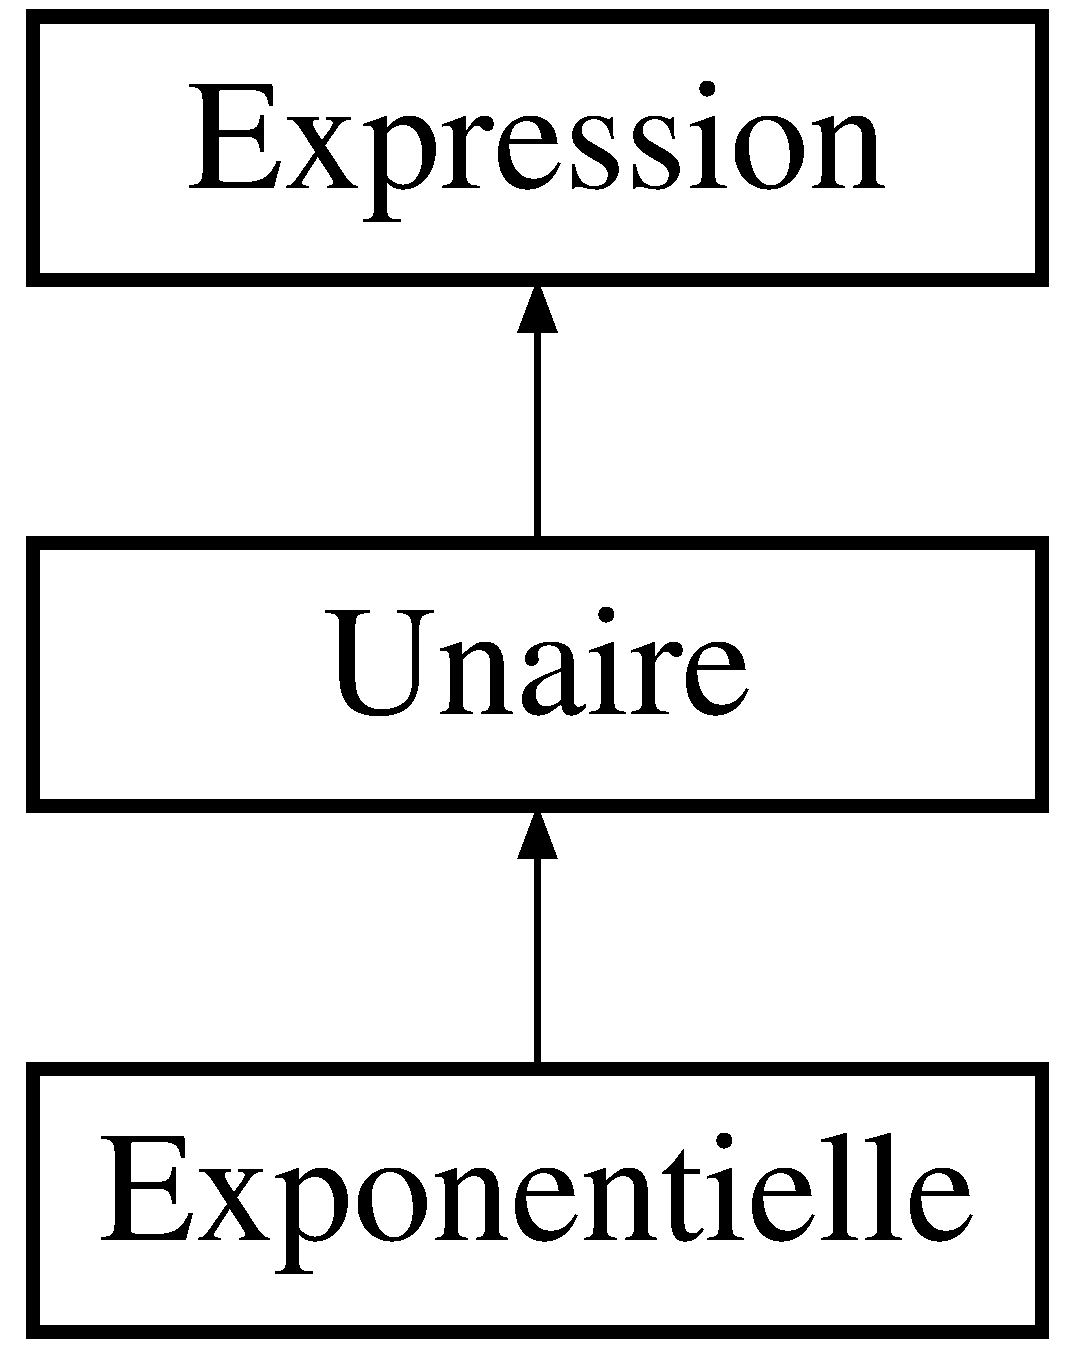
\includegraphics[height=3.000000cm]{class_exponentielle}
\end{center}
\end{figure}
\subsection*{Public Member Functions}
\begin{DoxyCompactItemize}
\item 
\hyperlink{class_exponentielle_a5a90ee0ae8bd1676e7b03ac56a939fae}{Exponentielle} ()
\begin{DoxyCompactList}\small\item\em Constructeur. \end{DoxyCompactList}\item 
\hyperlink{class_exponentielle_ab9207f0523e75c2008580d3b1633df44}{Exponentielle} (\hyperlink{class_expression}{Expression} $\ast$, \hyperlink{class_expression}{Expression} $\ast$, const string \&name=\char`\"{}ex\char`\"{})
\begin{DoxyCompactList}\small\item\em Constructeur. \end{DoxyCompactList}\item 
virtual \hyperlink{class_exponentielle_afedd0362a98f2b333cf7754b2b241a2c}{$\sim$\+Exponentielle} ()
\begin{DoxyCompactList}\small\item\em Destructeur Destructeur de la classe \hyperlink{class_affectation}{Affectation}. \end{DoxyCompactList}\item 
double \hyperlink{class_exponentielle_a8ef5b91ae85a4384d709266422d61c53}{eval} () const 
\begin{DoxyCompactList}\small\item\em Evalue l\textquotesingle{}expression Methode qui permet d\textquotesingle{}evaluer l\textquotesingle{}expression. \end{DoxyCompactList}\item 
\hyperlink{class_expression}{Expression} $\ast$ \hyperlink{class_exponentielle_a5937ff3e9a1f7af5c9bdd58ba5b21238}{deriver} (const string \&)
\begin{DoxyCompactList}\small\item\em Derive l\textquotesingle{}expression$\ast$ Methode qui permet deriver l\textquotesingle{}expression. \end{DoxyCompactList}\item 
\hyperlink{class_expression}{Expression} $\ast$ \hyperlink{class_exponentielle_a40634a92344070b2ac048de96052e33b}{simplifier} ()
\begin{DoxyCompactList}\small\item\em Simplifie l\textquotesingle{}expression Methode qui permet de simplifier l\textquotesingle{}expression. \end{DoxyCompactList}\item 
\hyperlink{class_expression}{Expression} $\ast$ \hyperlink{class_exponentielle_a670c2713c1b15db2b7eb703cb7f416c3}{clone} () const 
\begin{DoxyCompactList}\small\item\em clone l\textquotesingle{}expression Methode qui permet de cloner l\textquotesingle{}expression \end{DoxyCompactList}\item 
string \hyperlink{class_exponentielle_ae7391929f4181aa363e1c03e511c1263}{afficher} () const 
\begin{DoxyCompactList}\small\item\em Affiche l\textquotesingle{}expression Methode qui permet d\textquotesingle{}afficher l\textquotesingle{}expression. \end{DoxyCompactList}\end{DoxyCompactItemize}
\subsection*{Protected Attributes}
\begin{DoxyCompactItemize}
\item 
\hyperlink{class_expression}{Expression} $\ast$ \hyperlink{class_exponentielle_aa14b25a60e6d0f38607a37a999921363}{\+\_\+exp}
\item 
\hyperlink{class_expression}{Expression} $\ast$ \hyperlink{class_exponentielle_a3fb7904f3f814b94bcdf92d9cc4122fa}{\+\_\+pow}
\end{DoxyCompactItemize}
\subsection*{Friends}
\begin{DoxyCompactItemize}
\item 
ostream \& \hyperlink{class_exponentielle_a8514517e133bf4a16a23f882556c9bd3}{operator$<$$<$} (ostream \&, const \hyperlink{class_exponentielle}{Exponentielle} \&)
\begin{DoxyCompactList}\small\item\em operator$<$$<$ Methode qui permet d\textquotesingle{}afficher l\textquotesingle{}expression \end{DoxyCompactList}\end{DoxyCompactItemize}
\subsection*{Additional Inherited Members}


\subsection{Detailed Description}
La classe \hyperlink{class_exponentielle}{Exponentielle}. 

Cette classe repr�sente l\textquotesingle{}\hyperlink{class_exponentielle}{Exponentielle}. 

\subsection{Constructor \& Destructor Documentation}
\index{Exponentielle@{Exponentielle}!Exponentielle@{Exponentielle}}
\index{Exponentielle@{Exponentielle}!Exponentielle@{Exponentielle}}
\subsubsection[{\texorpdfstring{Exponentielle()}{Exponentielle()}}]{\setlength{\rightskip}{0pt plus 5cm}Exponentielle\+::\+Exponentielle (
\begin{DoxyParamCaption}
{}
\end{DoxyParamCaption}
)}\hypertarget{class_exponentielle_a5a90ee0ae8bd1676e7b03ac56a939fae}{}\label{class_exponentielle_a5a90ee0ae8bd1676e7b03ac56a939fae}


Constructeur. 

Constructeur de la classe \hyperlink{class_exponentielle}{Exponentielle} \index{Exponentielle@{Exponentielle}!Exponentielle@{Exponentielle}}
\index{Exponentielle@{Exponentielle}!Exponentielle@{Exponentielle}}
\subsubsection[{\texorpdfstring{Exponentielle(\+Expression $\ast$, Expression $\ast$, const string \&name=""ex"")}{Exponentielle(Expression *, Expression *, const string &name="ex")}}]{\setlength{\rightskip}{0pt plus 5cm}Exponentielle\+::\+Exponentielle (
\begin{DoxyParamCaption}
\item[{{\bf Expression} $\ast$}]{exp, }
\item[{{\bf Expression} $\ast$}]{pow, }
\item[{const string \&}]{name = {\ttfamily \char`\"{}ex\char`\"{}}}
\end{DoxyParamCaption}
)}\hypertarget{class_exponentielle_ab9207f0523e75c2008580d3b1633df44}{}\label{class_exponentielle_ab9207f0523e75c2008580d3b1633df44}


Constructeur. 

Constructeur de la classe \hyperlink{class_exponentielle}{Exponentielle}


\begin{DoxyParams}{Parameters}
{\em exp1} & \+: l\textquotesingle{}expression \\
\hline
{\em exp2} & \+: le puissance \\
\hline
{\em nom} & \+: le nom \\
\hline
\end{DoxyParams}
\index{Exponentielle@{Exponentielle}!````~Exponentielle@{$\sim$\+Exponentielle}}
\index{````~Exponentielle@{$\sim$\+Exponentielle}!Exponentielle@{Exponentielle}}
\subsubsection[{\texorpdfstring{$\sim$\+Exponentielle()}{~Exponentielle()}}]{\setlength{\rightskip}{0pt plus 5cm}Exponentielle\+::$\sim$\+Exponentielle (
\begin{DoxyParamCaption}
{}
\end{DoxyParamCaption}
)\hspace{0.3cm}{\ttfamily [virtual]}}\hypertarget{class_exponentielle_afedd0362a98f2b333cf7754b2b241a2c}{}\label{class_exponentielle_afedd0362a98f2b333cf7754b2b241a2c}


Destructeur Destructeur de la classe \hyperlink{class_affectation}{Affectation}. 



\subsection{Member Function Documentation}
\index{Exponentielle@{Exponentielle}!afficher@{afficher}}
\index{afficher@{afficher}!Exponentielle@{Exponentielle}}
\subsubsection[{\texorpdfstring{afficher() const }{afficher() const }}]{\setlength{\rightskip}{0pt plus 5cm}string Exponentielle\+::afficher (
\begin{DoxyParamCaption}
{}
\end{DoxyParamCaption}
) const\hspace{0.3cm}{\ttfamily [virtual]}}\hypertarget{class_exponentielle_ae7391929f4181aa363e1c03e511c1263}{}\label{class_exponentielle_ae7391929f4181aa363e1c03e511c1263}


Affiche l\textquotesingle{}expression Methode qui permet d\textquotesingle{}afficher l\textquotesingle{}expression. 

\begin{DoxyReturn}{Returns}
Le string d\textquotesingle{}expression 
\end{DoxyReturn}


Reimplemented from \hyperlink{class_expression_a953c7de0302331023987a2fff895cb85}{Expression}.

\index{Exponentielle@{Exponentielle}!clone@{clone}}
\index{clone@{clone}!Exponentielle@{Exponentielle}}
\subsubsection[{\texorpdfstring{clone() const }{clone() const }}]{\setlength{\rightskip}{0pt plus 5cm}{\bf Expression} $\ast$ Exponentielle\+::clone (
\begin{DoxyParamCaption}
{}
\end{DoxyParamCaption}
) const\hspace{0.3cm}{\ttfamily [virtual]}}\hypertarget{class_exponentielle_a670c2713c1b15db2b7eb703cb7f416c3}{}\label{class_exponentielle_a670c2713c1b15db2b7eb703cb7f416c3}


clone l\textquotesingle{}expression Methode qui permet de cloner l\textquotesingle{}expression 

\begin{DoxyReturn}{Returns}
L\textquotesingle{}expression clon� 
\end{DoxyReturn}


Implements \hyperlink{class_expression_ac9fcea09ddd3a650a92c3606118abfb6}{Expression}.

\index{Exponentielle@{Exponentielle}!deriver@{deriver}}
\index{deriver@{deriver}!Exponentielle@{Exponentielle}}
\subsubsection[{\texorpdfstring{deriver(const string \&)}{deriver(const string &)}}]{\setlength{\rightskip}{0pt plus 5cm}{\bf Expression} $\ast$ Exponentielle\+::deriver (
\begin{DoxyParamCaption}
\item[{const string \&}]{var}
\end{DoxyParamCaption}
)\hspace{0.3cm}{\ttfamily [virtual]}}\hypertarget{class_exponentielle_a5937ff3e9a1f7af5c9bdd58ba5b21238}{}\label{class_exponentielle_a5937ff3e9a1f7af5c9bdd58ba5b21238}


Derive l\textquotesingle{}expression$\ast$ Methode qui permet deriver l\textquotesingle{}expression. 

\begin{DoxyReturn}{Returns}
L\textquotesingle{}expression deriv� 
\end{DoxyReturn}


Implements \hyperlink{class_expression_a0a2a2cf2cdb1e8ca556ad59832784193}{Expression}.

\index{Exponentielle@{Exponentielle}!eval@{eval}}
\index{eval@{eval}!Exponentielle@{Exponentielle}}
\subsubsection[{\texorpdfstring{eval() const }{eval() const }}]{\setlength{\rightskip}{0pt plus 5cm}double Exponentielle\+::eval (
\begin{DoxyParamCaption}
{}
\end{DoxyParamCaption}
) const\hspace{0.3cm}{\ttfamily [virtual]}}\hypertarget{class_exponentielle_a8ef5b91ae85a4384d709266422d61c53}{}\label{class_exponentielle_a8ef5b91ae85a4384d709266422d61c53}


Evalue l\textquotesingle{}expression Methode qui permet d\textquotesingle{}evaluer l\textquotesingle{}expression. 

\begin{DoxyReturn}{Returns}
Le valeur d\textquotesingle{}expression 
\end{DoxyReturn}


Implements \hyperlink{class_expression_a5481c36265e11eff513df87bbc5a1d33}{Expression}.

\index{Exponentielle@{Exponentielle}!simplifier@{simplifier}}
\index{simplifier@{simplifier}!Exponentielle@{Exponentielle}}
\subsubsection[{\texorpdfstring{simplifier()}{simplifier()}}]{\setlength{\rightskip}{0pt plus 5cm}{\bf Expression} $\ast$ Exponentielle\+::simplifier (
\begin{DoxyParamCaption}
{}
\end{DoxyParamCaption}
)\hspace{0.3cm}{\ttfamily [virtual]}}\hypertarget{class_exponentielle_a40634a92344070b2ac048de96052e33b}{}\label{class_exponentielle_a40634a92344070b2ac048de96052e33b}


Simplifie l\textquotesingle{}expression Methode qui permet de simplifier l\textquotesingle{}expression. 

\begin{DoxyReturn}{Returns}
L\textquotesingle{}expression simplifi� 
\end{DoxyReturn}


Implements \hyperlink{class_expression_a319d06d43ead325c835181419061ae0b}{Expression}.



\subsection{Friends And Related Function Documentation}
\index{Exponentielle@{Exponentielle}!operator$<$$<$@{operator$<$$<$}}
\index{operator$<$$<$@{operator$<$$<$}!Exponentielle@{Exponentielle}}
\subsubsection[{\texorpdfstring{operator$<$$<$}{operator<<}}]{\setlength{\rightskip}{0pt plus 5cm}ostream\& operator$<$$<$ (
\begin{DoxyParamCaption}
\item[{ostream \&}]{os, }
\item[{const {\bf Exponentielle} \&}]{a}
\end{DoxyParamCaption}
)\hspace{0.3cm}{\ttfamily [friend]}}\hypertarget{class_exponentielle_a8514517e133bf4a16a23f882556c9bd3}{}\label{class_exponentielle_a8514517e133bf4a16a23f882556c9bd3}


operator$<$$<$ Methode qui permet d\textquotesingle{}afficher l\textquotesingle{}expression 



\subsection{Member Data Documentation}
\index{Exponentielle@{Exponentielle}!\+\_\+exp@{\+\_\+exp}}
\index{\+\_\+exp@{\+\_\+exp}!Exponentielle@{Exponentielle}}
\subsubsection[{\texorpdfstring{\+\_\+exp}{_exp}}]{\setlength{\rightskip}{0pt plus 5cm}{\bf Expression}$\ast$ Exponentielle\+::\+\_\+exp\hspace{0.3cm}{\ttfamily [protected]}}\hypertarget{class_exponentielle_aa14b25a60e6d0f38607a37a999921363}{}\label{class_exponentielle_aa14b25a60e6d0f38607a37a999921363}
\index{Exponentielle@{Exponentielle}!\+\_\+pow@{\+\_\+pow}}
\index{\+\_\+pow@{\+\_\+pow}!Exponentielle@{Exponentielle}}
\subsubsection[{\texorpdfstring{\+\_\+pow}{_pow}}]{\setlength{\rightskip}{0pt plus 5cm}{\bf Expression}$\ast$ Exponentielle\+::\+\_\+pow\hspace{0.3cm}{\ttfamily [protected]}}\hypertarget{class_exponentielle_a3fb7904f3f814b94bcdf92d9cc4122fa}{}\label{class_exponentielle_a3fb7904f3f814b94bcdf92d9cc4122fa}


The documentation for this class was generated from the following files\+:\begin{DoxyCompactItemize}
\item 
include/\hyperlink{unaire_8h}{unaire.\+h}\item 
src/\hyperlink{unaire_8cpp}{unaire.\+cpp}\end{DoxyCompactItemize}

\hypertarget{class_expression}{}\section{Expression Class Reference}
\label{class_expression}\index{Expression@{Expression}}


La classe \hyperlink{class_expression}{Expression}.  




{\ttfamily \#include $<$expression.\+h$>$}

Inheritance diagram for Expression\+:\begin{figure}[H]
\begin{center}
\leavevmode
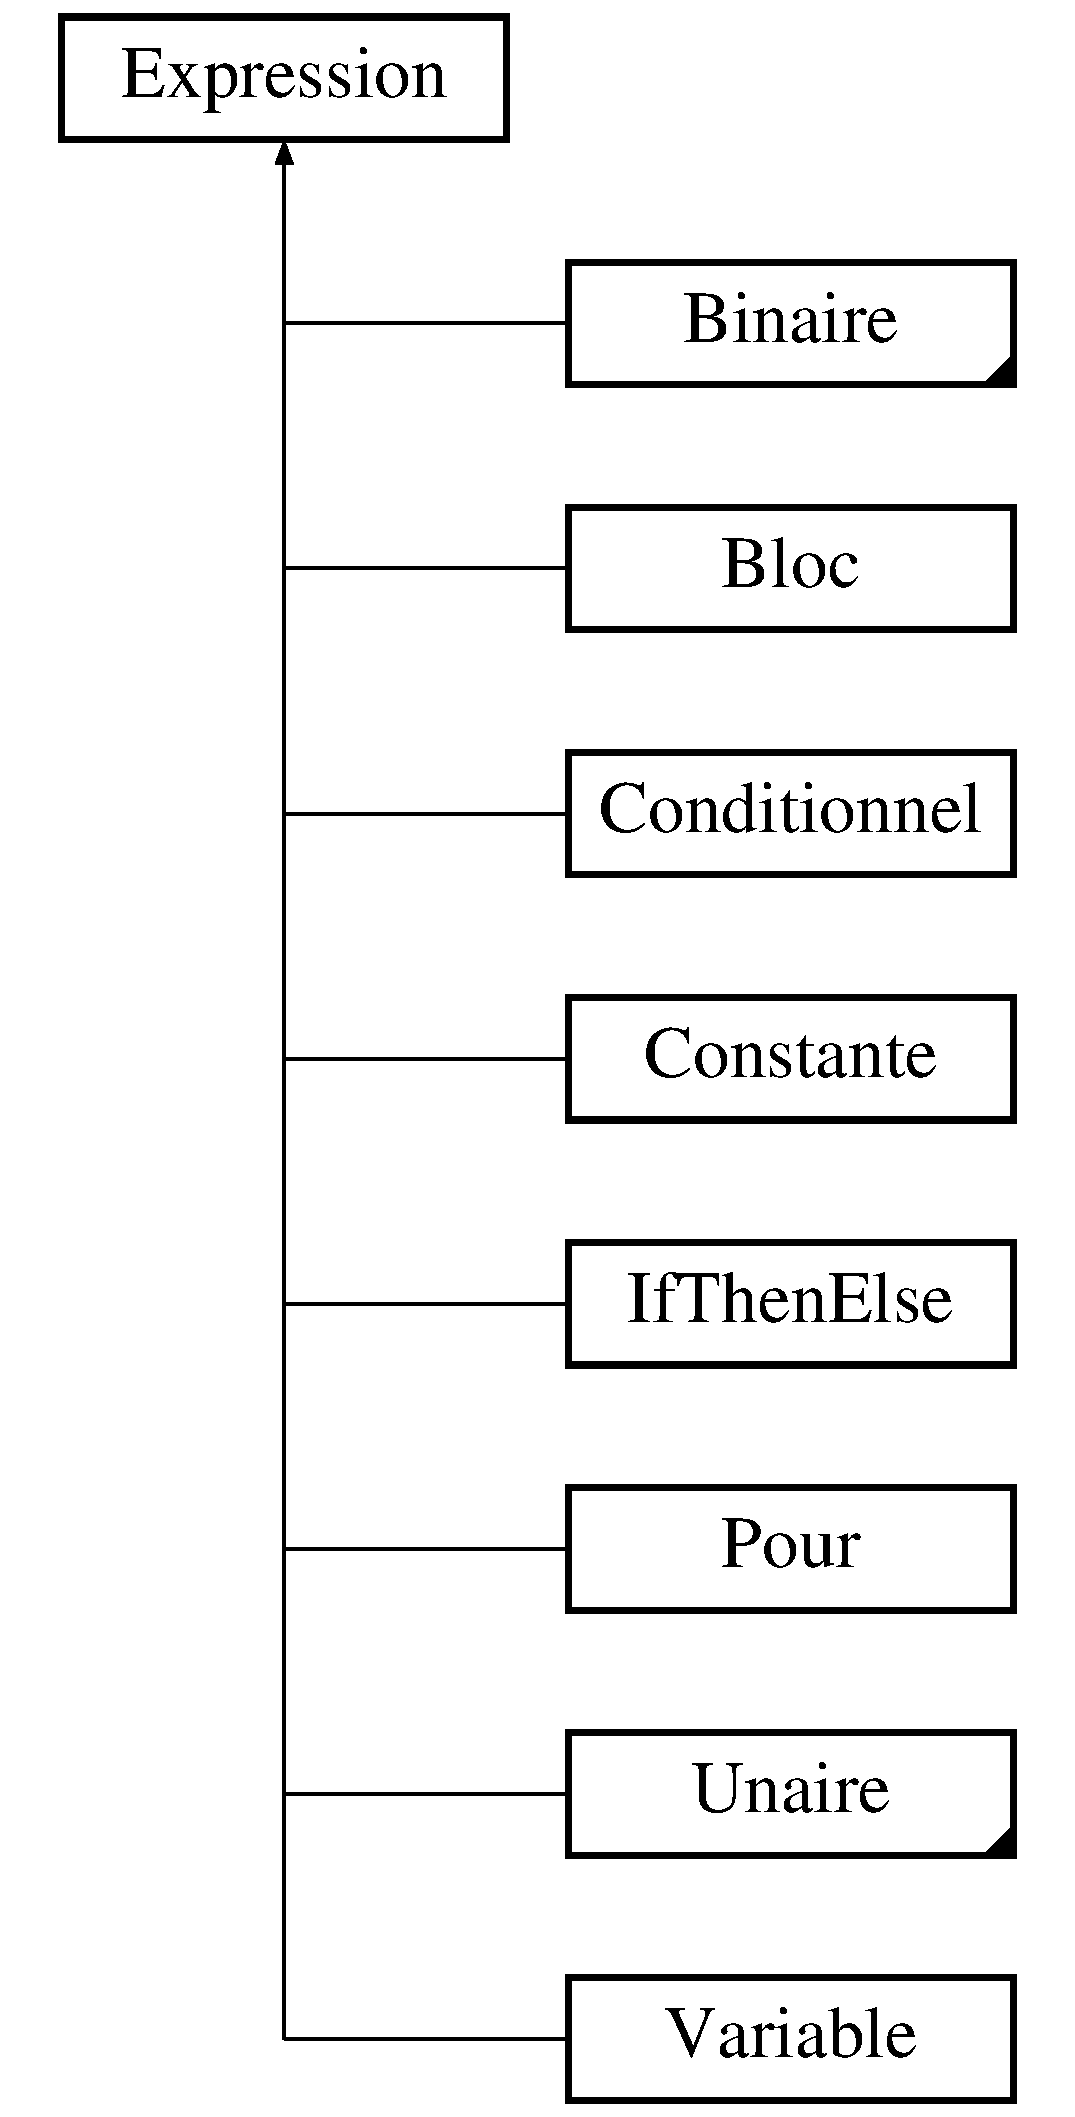
\includegraphics[height=9.000000cm]{class_expression}
\end{center}
\end{figure}
\subsection*{Public Member Functions}
\begin{DoxyCompactItemize}
\item 
\hyperlink{class_expression_afcf87716bf0abfe8d414c92529e1564a}{Expression} ()
\begin{DoxyCompactList}\small\item\em Constructeur. \end{DoxyCompactList}\item 
\hyperlink{class_expression_af356120f34980bb9b9b8f491f2b0913a}{Expression} (const string \&)
\begin{DoxyCompactList}\small\item\em Constructeur. \end{DoxyCompactList}\item 
virtual \hyperlink{class_expression_a3e99570b177da619eeb2c5787cbb148e}{$\sim$\+Expression} ()
\begin{DoxyCompactList}\small\item\em Destructeur Destructeur de la classe \hyperlink{class_affectation}{Affectation}. \end{DoxyCompactList}\item 
virtual string \hyperlink{class_expression_a953c7de0302331023987a2fff895cb85}{afficher} () const 
\begin{DoxyCompactList}\small\item\em Affiche l\textquotesingle{}expression Methode qui permet d\textquotesingle{}afficher l\textquotesingle{}expression. \end{DoxyCompactList}\item 
virtual \hyperlink{class_expression}{Expression} $\ast$ \hyperlink{class_expression_ac9fcea09ddd3a650a92c3606118abfb6}{clone} () const  =0
\begin{DoxyCompactList}\small\item\em clone l\textquotesingle{}expression Methode qui permet de cloner l\textquotesingle{}expression \end{DoxyCompactList}\item 
virtual \hyperlink{class_expression}{Expression} $\ast$ \hyperlink{class_expression_a0a2a2cf2cdb1e8ca556ad59832784193}{deriver} (const string \&)=0
\begin{DoxyCompactList}\small\item\em Derive l\textquotesingle{}expression$\ast$ Methode qui permet deriver l\textquotesingle{}expression. \end{DoxyCompactList}\item 
virtual \hyperlink{class_expression}{Expression} $\ast$ \hyperlink{class_expression_a319d06d43ead325c835181419061ae0b}{simplifier} ()=0
\begin{DoxyCompactList}\small\item\em Simplifie l\textquotesingle{}expression Methode qui permet de simplifier l\textquotesingle{}expression. \end{DoxyCompactList}\item 
virtual double \hyperlink{class_expression_a5481c36265e11eff513df87bbc5a1d33}{eval} () const  =0
\begin{DoxyCompactList}\small\item\em Evalue l\textquotesingle{}expression Methode qui permet d\textquotesingle{}evaluer l\textquotesingle{}expression. \end{DoxyCompactList}\end{DoxyCompactItemize}
\subsection*{Static Public Member Functions}
\begin{DoxyCompactItemize}
\item 
static void \hyperlink{class_expression_a6e403e2450258e3924aea969740205f4}{tout\+Liberer} ()
\end{DoxyCompactItemize}
\subsection*{Protected Attributes}
\begin{DoxyCompactItemize}
\item 
string \hyperlink{class_expression_aac494983d284346f05c4386bdbc65e56}{\+\_\+nom}
\end{DoxyCompactItemize}
\subsection*{Friends}
\begin{DoxyCompactItemize}
\item 
ostream \& \hyperlink{class_expression_afd5a48d1dc944d5594b5fba79c7ba263}{operator$<$$<$} (ostream \&, const \hyperlink{class_expression}{Expression} \&)
\begin{DoxyCompactList}\small\item\em operator$<$$<$ Methode qui permet d\textquotesingle{}afficher l\textquotesingle{}expression \end{DoxyCompactList}\end{DoxyCompactItemize}


\subsection{Detailed Description}
La classe \hyperlink{class_expression}{Expression}. 

Cette classe repr�sente l\textquotesingle{}expression 

\subsection{Constructor \& Destructor Documentation}
\index{Expression@{Expression}!Expression@{Expression}}
\index{Expression@{Expression}!Expression@{Expression}}
\subsubsection[{\texorpdfstring{Expression()}{Expression()}}]{\setlength{\rightskip}{0pt plus 5cm}Expression\+::\+Expression (
\begin{DoxyParamCaption}
{}
\end{DoxyParamCaption}
)}\hypertarget{class_expression_afcf87716bf0abfe8d414c92529e1564a}{}\label{class_expression_afcf87716bf0abfe8d414c92529e1564a}


Constructeur. 

Constructeur de la classe \hyperlink{class_expression}{Expression} \index{Expression@{Expression}!Expression@{Expression}}
\index{Expression@{Expression}!Expression@{Expression}}
\subsubsection[{\texorpdfstring{Expression(const string \&)}{Expression(const string &)}}]{\setlength{\rightskip}{0pt plus 5cm}Expression\+::\+Expression (
\begin{DoxyParamCaption}
\item[{const string \&}]{nom}
\end{DoxyParamCaption}
)}\hypertarget{class_expression_af356120f34980bb9b9b8f491f2b0913a}{}\label{class_expression_af356120f34980bb9b9b8f491f2b0913a}


Constructeur. 

Constructeur de la classe \hyperlink{class_expression}{Expression}


\begin{DoxyParams}{Parameters}
{\em nom} & \+: le nom d\textquotesingle{}expression \\
\hline
\end{DoxyParams}
\index{Expression@{Expression}!````~Expression@{$\sim$\+Expression}}
\index{````~Expression@{$\sim$\+Expression}!Expression@{Expression}}
\subsubsection[{\texorpdfstring{$\sim$\+Expression()}{~Expression()}}]{\setlength{\rightskip}{0pt plus 5cm}Expression\+::$\sim$\+Expression (
\begin{DoxyParamCaption}
{}
\end{DoxyParamCaption}
)\hspace{0.3cm}{\ttfamily [virtual]}}\hypertarget{class_expression_a3e99570b177da619eeb2c5787cbb148e}{}\label{class_expression_a3e99570b177da619eeb2c5787cbb148e}


Destructeur Destructeur de la classe \hyperlink{class_affectation}{Affectation}. 



\subsection{Member Function Documentation}
\index{Expression@{Expression}!afficher@{afficher}}
\index{afficher@{afficher}!Expression@{Expression}}
\subsubsection[{\texorpdfstring{afficher() const }{afficher() const }}]{\setlength{\rightskip}{0pt plus 5cm}string Expression\+::afficher (
\begin{DoxyParamCaption}
{}
\end{DoxyParamCaption}
) const\hspace{0.3cm}{\ttfamily [virtual]}}\hypertarget{class_expression_a953c7de0302331023987a2fff895cb85}{}\label{class_expression_a953c7de0302331023987a2fff895cb85}


Affiche l\textquotesingle{}expression Methode qui permet d\textquotesingle{}afficher l\textquotesingle{}expression. 

\begin{DoxyReturn}{Returns}
Le string d\textquotesingle{}expression 
\end{DoxyReturn}


Reimplemented in \hyperlink{class_inferieur_egal_a820821cedaab1a0bce1d13f49c55a006}{Inferieur\+Egal}, \hyperlink{class_superieur_egal_a9fb8d0b7cdfb75361bae0a2fa8db06a0}{Superieur\+Egal}, \hyperlink{class_inferieur_ad826ba17b77bdb74d07cab07db30c472}{Inferieur}, \hyperlink{class_superieur_a0613c6dc4df0de7cf6a4be2e45bcf0ac}{Superieur}, \hyperlink{class_division_af4b4b119ddfb23fd84244ac4eb6b5388}{Division}, \hyperlink{class_produit_aabe10cf42ec4e382d7b577573bea69a1}{Produit}, \hyperlink{class_exponentielle_ae7391929f4181aa363e1c03e511c1263}{Exponentielle}, \hyperlink{class_difference_af06c097f3901551229b8a7b73bccb94b}{Difference}, \hyperlink{class_somme_a3605a67027a5d0f7dc8c7617d2b1edfc}{Somme}, \hyperlink{class_variable_a2ae42f5b49f09c593be81f301462f1b3}{Variable}, \hyperlink{class_affectation_a37acdac77acfb27d8c59abfdbd5ed3b0}{Affectation}, \hyperlink{class_constante_a798db3847c1a81a68321cada88f3f43d}{Constante}, \hyperlink{class_conditionnel_ace6f0a27597c614b82a0f84a329167cf}{Conditionnel}, \hyperlink{class_bloc_acfe2075a0f69de800f447c1bc0aee63f}{Bloc}, \hyperlink{class_if_then_else_a25ca7b935d19e330c2502051f4791655}{If\+Then\+Else}, and \hyperlink{class_pour_a7d59b36e80ca85da59c4f5d93ffb674e}{Pour}.

\index{Expression@{Expression}!clone@{clone}}
\index{clone@{clone}!Expression@{Expression}}
\subsubsection[{\texorpdfstring{clone() const  =0}{clone() const  =0}}]{\setlength{\rightskip}{0pt plus 5cm}virtual {\bf Expression}$\ast$ Expression\+::clone (
\begin{DoxyParamCaption}
{}
\end{DoxyParamCaption}
) const\hspace{0.3cm}{\ttfamily [pure virtual]}}\hypertarget{class_expression_ac9fcea09ddd3a650a92c3606118abfb6}{}\label{class_expression_ac9fcea09ddd3a650a92c3606118abfb6}


clone l\textquotesingle{}expression Methode qui permet de cloner l\textquotesingle{}expression 

\begin{DoxyReturn}{Returns}
L\textquotesingle{}expression clon� 
\end{DoxyReturn}


Implemented in \hyperlink{class_inferieur_egal_acdeb552ab7486e0cabe0af7a7e0f4b6c}{Inferieur\+Egal}, \hyperlink{class_superieur_egal_a55d16bacf7aff0cf9c8a7b4992b09279}{Superieur\+Egal}, \hyperlink{class_inferieur_afdf1b8ba0a235bc1329923ac0fe61fbb}{Inferieur}, \hyperlink{class_superieur_a13e12cfa91154853de73d67518fb7795}{Superieur}, \hyperlink{class_division_a810f31960659e2a95ddfe4f49e08cb99}{Division}, \hyperlink{class_produit_a6fed59a3d22b91d80c59d6fd664c122c}{Produit}, \hyperlink{class_exponentielle_a670c2713c1b15db2b7eb703cb7f416c3}{Exponentielle}, \hyperlink{class_difference_a3bd254abd06c7ed2b6946c7682bec584}{Difference}, \hyperlink{class_cos_a1c4eb6ff08383ac08e7b511aa9d50fb2}{Cos}, \hyperlink{class_somme_aaf95e8388a3eb28edddd205805d9c10b}{Somme}, \hyperlink{class_sin_a12ca12d6edd6a6d98566b1befef978c4}{Sin}, \hyperlink{class_variable_a0862fa73db06e1c7f6fdd82dd7c3fc24}{Variable}, \hyperlink{class_affectation_aef2d294e0ab788aace81d33097a80d18}{Affectation}, \hyperlink{class_constante_a3227e53212fc8381fb33c559b22b868d}{Constante}, \hyperlink{class_conditionnel_a3dec2cad7a9a43495c4bdc2b6b65f4a4}{Conditionnel}, \hyperlink{class_bloc_a15c01c71bdad5b42c2d79102a19ca5aa}{Bloc}, \hyperlink{class_if_then_else_aba998c96619eeb1d2d29fccf9350a095}{If\+Then\+Else}, and \hyperlink{class_pour_a0116d7b9233b8b9dd48999f781f4592f}{Pour}.

\index{Expression@{Expression}!deriver@{deriver}}
\index{deriver@{deriver}!Expression@{Expression}}
\subsubsection[{\texorpdfstring{deriver(const string \&)=0}{deriver(const string &)=0}}]{\setlength{\rightskip}{0pt plus 5cm}{\bf Expression} $\ast$ Expression\+::deriver (
\begin{DoxyParamCaption}
\item[{const string \&}]{}
\end{DoxyParamCaption}
)\hspace{0.3cm}{\ttfamily [pure virtual]}}\hypertarget{class_expression_a0a2a2cf2cdb1e8ca556ad59832784193}{}\label{class_expression_a0a2a2cf2cdb1e8ca556ad59832784193}


Derive l\textquotesingle{}expression$\ast$ Methode qui permet deriver l\textquotesingle{}expression. 

\begin{DoxyReturn}{Returns}
L\textquotesingle{}expression deriv� 
\end{DoxyReturn}


Implemented in \hyperlink{class_inferieur_egal_af3dfc429ad45e2ed60920e423f363e46}{Inferieur\+Egal}, \hyperlink{class_superieur_egal_ae1aa499c6130c12a96910df1f6776fac}{Superieur\+Egal}, \hyperlink{class_inferieur_a40bd4ec1d76deef074b97c6f0959606f}{Inferieur}, \hyperlink{class_superieur_a316ead2ea4d6451a6056947bd4f3cdbd}{Superieur}, \hyperlink{class_division_addfc9004319763a3fc8a2ead6d02151c}{Division}, \hyperlink{class_produit_a8aa9088f34b20414cec38451f43f0520}{Produit}, \hyperlink{class_exponentielle_a5937ff3e9a1f7af5c9bdd58ba5b21238}{Exponentielle}, \hyperlink{class_difference_af9118a276538e992bff5dfcae3d3b25f}{Difference}, \hyperlink{class_cos_a23bcff67edb0140231ea0b00f68f9a3a}{Cos}, \hyperlink{class_sin_a62c81e668f29b126f7fcc6ed4e6fb4dc}{Sin}, \hyperlink{class_somme_a6288da4022b7ee227431e0531ddd4664}{Somme}, \hyperlink{class_conditionnel_ac7ac864a499c05d874ab88dbb4bda442}{Conditionnel}, \hyperlink{class_bloc_ad8547a697be0d0829fbf13d4f6623376}{Bloc}, \hyperlink{class_if_then_else_a7fe544a73f42777341df653b290116d5}{If\+Then\+Else}, \hyperlink{class_pour_a6bd2f404e8531dca015c05edced0a63e}{Pour}, \hyperlink{class_variable_ae7e8e77718b47b10f7633756715aa986}{Variable}, \hyperlink{class_affectation_a918e2a05678e29ee1b7172e8eec95083}{Affectation}, and \hyperlink{class_constante_a78c242a323b89ebc7b1ffdd817e2bd76}{Constante}.

\index{Expression@{Expression}!eval@{eval}}
\index{eval@{eval}!Expression@{Expression}}
\subsubsection[{\texorpdfstring{eval() const  =0}{eval() const  =0}}]{\setlength{\rightskip}{0pt plus 5cm}double Expression\+::eval (
\begin{DoxyParamCaption}
{}
\end{DoxyParamCaption}
) const\hspace{0.3cm}{\ttfamily [pure virtual]}}\hypertarget{class_expression_a5481c36265e11eff513df87bbc5a1d33}{}\label{class_expression_a5481c36265e11eff513df87bbc5a1d33}


Evalue l\textquotesingle{}expression Methode qui permet d\textquotesingle{}evaluer l\textquotesingle{}expression. 

\begin{DoxyReturn}{Returns}
Le valeur d\textquotesingle{}expression 
\end{DoxyReturn}


Implemented in \hyperlink{class_inferieur_egal_aece49b421f83e80f33eb43adec758cdd}{Inferieur\+Egal}, \hyperlink{class_superieur_egal_a1ea7bc313de485e4055914661d5e596a}{Superieur\+Egal}, \hyperlink{class_inferieur_a8b4e8f22ab48859ad781f1997b083d46}{Inferieur}, \hyperlink{class_superieur_aee2a8239ebc62ae3db015d2744013fb7}{Superieur}, \hyperlink{class_division_a58dbaea10d63a27367155141cb9db323}{Division}, \hyperlink{class_produit_a6c4efb337679a2cf7ea920c95616d7fe}{Produit}, \hyperlink{class_exponentielle_a8ef5b91ae85a4384d709266422d61c53}{Exponentielle}, \hyperlink{class_difference_a0da9cd3169bea5ca70af3f4aed9a55a8}{Difference}, \hyperlink{class_cos_a601f93938da00a524c3cce3a9bcc6c7d}{Cos}, \hyperlink{class_sin_a12366e0380d5f03f5a83b09a6b861b35}{Sin}, \hyperlink{class_somme_ab36403713c60f51ee6eebc5693ce3891}{Somme}, \hyperlink{class_conditionnel_a1421ef0258647e5c85a1fb2dc8a9434f}{Conditionnel}, \hyperlink{class_bloc_a8847a4df7adf319e48ed7a277347ac80}{Bloc}, \hyperlink{class_if_then_else_a67b94d8e5d88d2d13e90a296c58d2341}{If\+Then\+Else}, \hyperlink{class_pour_a19f811e4a5d7847cf635f389b09c9e39}{Pour}, \hyperlink{class_variable_a4bb6309ec2c117c5c050ca89488daf2e}{Variable}, \hyperlink{class_affectation_ad66950c792ad4ccf0e6491f55a7eaad2}{Affectation}, and \hyperlink{class_constante_aaf4b67f9a9d34aca1f689e6fbf63be75}{Constante}.

\index{Expression@{Expression}!simplifier@{simplifier}}
\index{simplifier@{simplifier}!Expression@{Expression}}
\subsubsection[{\texorpdfstring{simplifier()=0}{simplifier()=0}}]{\setlength{\rightskip}{0pt plus 5cm}virtual {\bf Expression}$\ast$ Expression\+::simplifier (
\begin{DoxyParamCaption}
{}
\end{DoxyParamCaption}
)\hspace{0.3cm}{\ttfamily [pure virtual]}}\hypertarget{class_expression_a319d06d43ead325c835181419061ae0b}{}\label{class_expression_a319d06d43ead325c835181419061ae0b}


Simplifie l\textquotesingle{}expression Methode qui permet de simplifier l\textquotesingle{}expression. 

\begin{DoxyReturn}{Returns}
L\textquotesingle{}expression simplifi� 
\end{DoxyReturn}


Implemented in \hyperlink{class_inferieur_egal_a65e16573f97d5073fb43c7c91a43e5d3}{Inferieur\+Egal}, \hyperlink{class_superieur_egal_a8df045c9b0a436106ccc3e51b7d7d21d}{Superieur\+Egal}, \hyperlink{class_inferieur_a08e1dcb1007cdff4e5fc9303da1df1f3}{Inferieur}, \hyperlink{class_superieur_abdf12b4d6d2a36a36ee48556c674aa00}{Superieur}, \hyperlink{class_division_acf3fafff49eb477ca7f4f84b9c5519f3}{Division}, \hyperlink{class_produit_a4b4db95c687fb3d949e67f7b81e9e9ee}{Produit}, \hyperlink{class_exponentielle_a40634a92344070b2ac048de96052e33b}{Exponentielle}, \hyperlink{class_difference_a1ea49952e410f10cc4907e80ac2597d4}{Difference}, \hyperlink{class_cos_ae22a7bd0a5caf0cab864f80e954ecd34}{Cos}, \hyperlink{class_sin_aa988c5b6f05d2452975ed35125b4fa08}{Sin}, \hyperlink{class_somme_a486f0b09a4697593b638486428b849f3}{Somme}, \hyperlink{class_conditionnel_adafd38733d1384a44f981a292f234e1f}{Conditionnel}, \hyperlink{class_bloc_afd5d437c0b31109b90946d183a150642}{Bloc}, \hyperlink{class_if_then_else_ab16dd963e35a71525ffecffffe338ed3}{If\+Then\+Else}, \hyperlink{class_pour_a7a03702950b98e370df5fb8ae3ab5417}{Pour}, \hyperlink{class_variable_a60c5ae49c674293b68646342c9de242f}{Variable}, \hyperlink{class_affectation_ac39339edc60e2f44edf0cc8ec94e4313}{Affectation}, and \hyperlink{class_constante_a6e034b3b42fbcfcee505303648c03d69}{Constante}.

\index{Expression@{Expression}!tout\+Liberer@{tout\+Liberer}}
\index{tout\+Liberer@{tout\+Liberer}!Expression@{Expression}}
\subsubsection[{\texorpdfstring{tout\+Liberer()}{toutLiberer()}}]{\setlength{\rightskip}{0pt plus 5cm}void Expression\+::tout\+Liberer (
\begin{DoxyParamCaption}
{}
\end{DoxyParamCaption}
)\hspace{0.3cm}{\ttfamily [static]}}\hypertarget{class_expression_a6e403e2450258e3924aea969740205f4}{}\label{class_expression_a6e403e2450258e3924aea969740205f4}


\subsection{Friends And Related Function Documentation}
\index{Expression@{Expression}!operator$<$$<$@{operator$<$$<$}}
\index{operator$<$$<$@{operator$<$$<$}!Expression@{Expression}}
\subsubsection[{\texorpdfstring{operator$<$$<$}{operator<<}}]{\setlength{\rightskip}{0pt plus 5cm}ostream\& operator$<$$<$ (
\begin{DoxyParamCaption}
\item[{ostream \&}]{os, }
\item[{const {\bf Expression} \&}]{a}
\end{DoxyParamCaption}
)\hspace{0.3cm}{\ttfamily [friend]}}\hypertarget{class_expression_afd5a48d1dc944d5594b5fba79c7ba263}{}\label{class_expression_afd5a48d1dc944d5594b5fba79c7ba263}


operator$<$$<$ Methode qui permet d\textquotesingle{}afficher l\textquotesingle{}expression 



\subsection{Member Data Documentation}
\index{Expression@{Expression}!\+\_\+nom@{\+\_\+nom}}
\index{\+\_\+nom@{\+\_\+nom}!Expression@{Expression}}
\subsubsection[{\texorpdfstring{\+\_\+nom}{_nom}}]{\setlength{\rightskip}{0pt plus 5cm}string Expression\+::\+\_\+nom\hspace{0.3cm}{\ttfamily [protected]}}\hypertarget{class_expression_aac494983d284346f05c4386bdbc65e56}{}\label{class_expression_aac494983d284346f05c4386bdbc65e56}


The documentation for this class was generated from the following files\+:\begin{DoxyCompactItemize}
\item 
include/\hyperlink{expression_8h}{expression.\+h}\item 
src/\hyperlink{expression_8cpp}{expression.\+cpp}\end{DoxyCompactItemize}

\hypertarget{class_if_then_else}{}\section{If\+Then\+Else Class Reference}
\label{class_if_then_else}\index{If\+Then\+Else@{If\+Then\+Else}}


La classe \hyperlink{class_if_then_else}{If\+Then\+Else}.  




{\ttfamily \#include $<$if\+Then\+Else.\+h$>$}

Inheritance diagram for If\+Then\+Else\+:\begin{figure}[H]
\begin{center}
\leavevmode
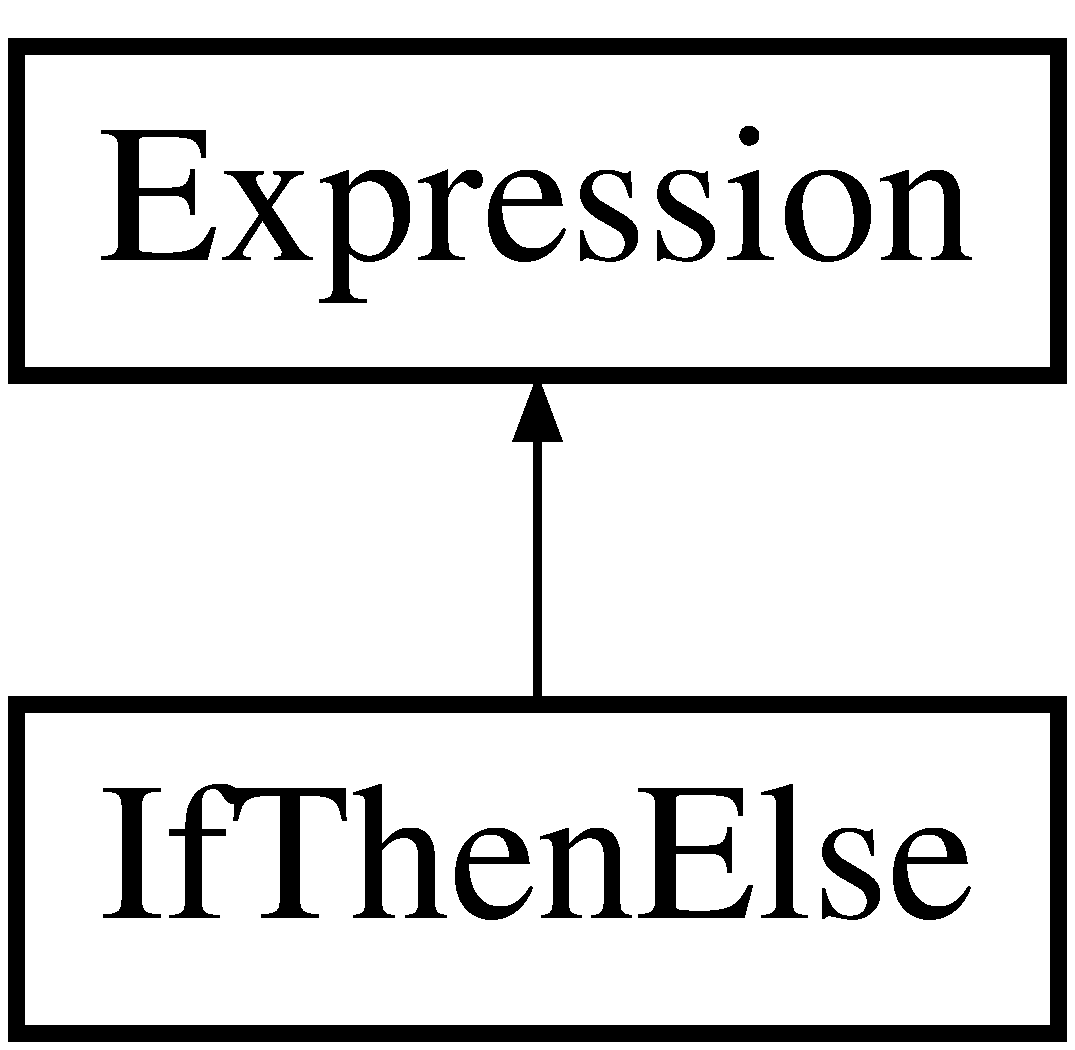
\includegraphics[height=2.000000cm]{class_if_then_else}
\end{center}
\end{figure}
\subsection*{Public Member Functions}
\begin{DoxyCompactItemize}
\item 
\hyperlink{class_if_then_else_a110b5dc89a5cc24d48b3ce61f30e9834}{If\+Then\+Else} ()
\begin{DoxyCompactList}\small\item\em Constructeur. \end{DoxyCompactList}\item 
virtual \hyperlink{class_if_then_else_a14d1c1cea52dd3b9939de1e6b54b86c6}{$\sim$\+If\+Then\+Else} ()
\begin{DoxyCompactList}\small\item\em Destructeur Destructeur de la classe \hyperlink{class_affectation}{Affectation}. \end{DoxyCompactList}\item 
\hyperlink{class_if_then_else_a38e9daf3a0d1d80ca3a42a0a63cda9c3}{If\+Then\+Else} (\hyperlink{class_binaire}{Binaire} $\ast$, \hyperlink{class_expression}{Expression} $\ast$, \hyperlink{class_expression}{Expression} $\ast$)
\begin{DoxyCompactList}\small\item\em Constructeur. \end{DoxyCompactList}\item 
\hyperlink{class_expression}{Expression} $\ast$ \hyperlink{class_if_then_else_aba998c96619eeb1d2d29fccf9350a095}{clone} () const 
\begin{DoxyCompactList}\small\item\em clone l\textquotesingle{}expression Methode qui permet de cloner l\textquotesingle{}expression \end{DoxyCompactList}\item 
string \hyperlink{class_if_then_else_a25ca7b935d19e330c2502051f4791655}{afficher} () const 
\begin{DoxyCompactList}\small\item\em Affiche l\textquotesingle{}expression Methode qui permet d\textquotesingle{}afficher l\textquotesingle{}expression. \end{DoxyCompactList}\item 
double \hyperlink{class_if_then_else_a67b94d8e5d88d2d13e90a296c58d2341}{eval} () const 
\begin{DoxyCompactList}\small\item\em Evalue l\textquotesingle{}expression Methode qui permet d\textquotesingle{}evaluer l\textquotesingle{}expression. \end{DoxyCompactList}\item 
\hyperlink{class_expression}{Expression} $\ast$ \hyperlink{class_if_then_else_a7fe544a73f42777341df653b290116d5}{deriver} (const string \&)
\begin{DoxyCompactList}\small\item\em Derive l\textquotesingle{}expression$\ast$ Methode qui permet deriver l\textquotesingle{}expression. \end{DoxyCompactList}\item 
\hyperlink{class_expression}{Expression} $\ast$ \hyperlink{class_if_then_else_ab16dd963e35a71525ffecffffe338ed3}{simplifier} ()
\begin{DoxyCompactList}\small\item\em Simplifie l\textquotesingle{}expression Methode qui permet de simplifier l\textquotesingle{}expression. \end{DoxyCompactList}\end{DoxyCompactItemize}
\subsection*{Friends}
\begin{DoxyCompactItemize}
\item 
ostream \& \hyperlink{class_if_then_else_a0d8a32ab1c475d199aeec7b674b1481b}{operator$<$$<$} (ostream \&os, const \hyperlink{class_if_then_else}{If\+Then\+Else} \&)
\begin{DoxyCompactList}\small\item\em operator$<$$<$ Methode qui permet d\textquotesingle{}afficher l\textquotesingle{}expression \end{DoxyCompactList}\end{DoxyCompactItemize}
\subsection*{Additional Inherited Members}


\subsection{Detailed Description}
La classe \hyperlink{class_if_then_else}{If\+Then\+Else}. 

Cette classe repr�sente les structures de contr�le conditionnelles. Ils permettent d�ex�cuter une s�rie d\textquotesingle{}instructions dans le cas o� une condition est vraie, et d\textquotesingle{}ex�cuter une autre s�rie d\textquotesingle{}instructions dans le cas contraire. 

\subsection{Constructor \& Destructor Documentation}
\index{If\+Then\+Else@{If\+Then\+Else}!If\+Then\+Else@{If\+Then\+Else}}
\index{If\+Then\+Else@{If\+Then\+Else}!If\+Then\+Else@{If\+Then\+Else}}
\subsubsection[{\texorpdfstring{If\+Then\+Else()}{IfThenElse()}}]{\setlength{\rightskip}{0pt plus 5cm}If\+Then\+Else\+::\+If\+Then\+Else (
\begin{DoxyParamCaption}
{}
\end{DoxyParamCaption}
)}\hypertarget{class_if_then_else_a110b5dc89a5cc24d48b3ce61f30e9834}{}\label{class_if_then_else_a110b5dc89a5cc24d48b3ce61f30e9834}


Constructeur. 

Constructeur de la classe \hyperlink{class_if_then_else}{If\+Then\+Else} \index{If\+Then\+Else@{If\+Then\+Else}!````~If\+Then\+Else@{$\sim$\+If\+Then\+Else}}
\index{````~If\+Then\+Else@{$\sim$\+If\+Then\+Else}!If\+Then\+Else@{If\+Then\+Else}}
\subsubsection[{\texorpdfstring{$\sim$\+If\+Then\+Else()}{~IfThenElse()}}]{\setlength{\rightskip}{0pt plus 5cm}If\+Then\+Else\+::$\sim$\+If\+Then\+Else (
\begin{DoxyParamCaption}
{}
\end{DoxyParamCaption}
)\hspace{0.3cm}{\ttfamily [virtual]}}\hypertarget{class_if_then_else_a14d1c1cea52dd3b9939de1e6b54b86c6}{}\label{class_if_then_else_a14d1c1cea52dd3b9939de1e6b54b86c6}


Destructeur Destructeur de la classe \hyperlink{class_affectation}{Affectation}. 

\index{If\+Then\+Else@{If\+Then\+Else}!If\+Then\+Else@{If\+Then\+Else}}
\index{If\+Then\+Else@{If\+Then\+Else}!If\+Then\+Else@{If\+Then\+Else}}
\subsubsection[{\texorpdfstring{If\+Then\+Else(\+Binaire $\ast$, Expression $\ast$, Expression $\ast$)}{IfThenElse(Binaire *, Expression *, Expression *)}}]{\setlength{\rightskip}{0pt plus 5cm}If\+Then\+Else\+::\+If\+Then\+Else (
\begin{DoxyParamCaption}
\item[{{\bf Binaire} $\ast$}]{cond, }
\item[{{\bf Expression} $\ast$}]{exp1, }
\item[{{\bf Expression} $\ast$}]{exp2}
\end{DoxyParamCaption}
)}\hypertarget{class_if_then_else_a38e9daf3a0d1d80ca3a42a0a63cda9c3}{}\label{class_if_then_else_a38e9daf3a0d1d80ca3a42a0a63cda9c3}


Constructeur. 

Constructeur de la classe \hyperlink{class_if_then_else}{If\+Then\+Else}


\begin{DoxyParams}{Parameters}
{\em cond} & \+: le condition \\
\hline
{\em exp1} & \+: l\textquotesingle{}expression si la condition est vraie \\
\hline
{\em exp2} & \+: l\textquotesingle{}expression si la condition est fausse \\
\hline
\end{DoxyParams}


\subsection{Member Function Documentation}
\index{If\+Then\+Else@{If\+Then\+Else}!afficher@{afficher}}
\index{afficher@{afficher}!If\+Then\+Else@{If\+Then\+Else}}
\subsubsection[{\texorpdfstring{afficher() const }{afficher() const }}]{\setlength{\rightskip}{0pt plus 5cm}string If\+Then\+Else\+::afficher (
\begin{DoxyParamCaption}
{}
\end{DoxyParamCaption}
) const\hspace{0.3cm}{\ttfamily [virtual]}}\hypertarget{class_if_then_else_a25ca7b935d19e330c2502051f4791655}{}\label{class_if_then_else_a25ca7b935d19e330c2502051f4791655}


Affiche l\textquotesingle{}expression Methode qui permet d\textquotesingle{}afficher l\textquotesingle{}expression. 

\begin{DoxyReturn}{Returns}
Le string d\textquotesingle{}expression 
\end{DoxyReturn}


Reimplemented from \hyperlink{class_expression_a953c7de0302331023987a2fff895cb85}{Expression}.

\index{If\+Then\+Else@{If\+Then\+Else}!clone@{clone}}
\index{clone@{clone}!If\+Then\+Else@{If\+Then\+Else}}
\subsubsection[{\texorpdfstring{clone() const }{clone() const }}]{\setlength{\rightskip}{0pt plus 5cm}{\bf Expression} $\ast$ If\+Then\+Else\+::clone (
\begin{DoxyParamCaption}
{}
\end{DoxyParamCaption}
) const\hspace{0.3cm}{\ttfamily [virtual]}}\hypertarget{class_if_then_else_aba998c96619eeb1d2d29fccf9350a095}{}\label{class_if_then_else_aba998c96619eeb1d2d29fccf9350a095}


clone l\textquotesingle{}expression Methode qui permet de cloner l\textquotesingle{}expression 

\begin{DoxyReturn}{Returns}
L\textquotesingle{}expression clon� 
\end{DoxyReturn}


Implements \hyperlink{class_expression_ac9fcea09ddd3a650a92c3606118abfb6}{Expression}.

\index{If\+Then\+Else@{If\+Then\+Else}!deriver@{deriver}}
\index{deriver@{deriver}!If\+Then\+Else@{If\+Then\+Else}}
\subsubsection[{\texorpdfstring{deriver(const string \&)}{deriver(const string &)}}]{\setlength{\rightskip}{0pt plus 5cm}{\bf Expression} $\ast$ If\+Then\+Else\+::deriver (
\begin{DoxyParamCaption}
\item[{const string \&}]{var}
\end{DoxyParamCaption}
)\hspace{0.3cm}{\ttfamily [virtual]}}\hypertarget{class_if_then_else_a7fe544a73f42777341df653b290116d5}{}\label{class_if_then_else_a7fe544a73f42777341df653b290116d5}


Derive l\textquotesingle{}expression$\ast$ Methode qui permet deriver l\textquotesingle{}expression. 

\begin{DoxyReturn}{Returns}
L\textquotesingle{}expression deriv� 
\end{DoxyReturn}


Implements \hyperlink{class_expression_a0a2a2cf2cdb1e8ca556ad59832784193}{Expression}.

\index{If\+Then\+Else@{If\+Then\+Else}!eval@{eval}}
\index{eval@{eval}!If\+Then\+Else@{If\+Then\+Else}}
\subsubsection[{\texorpdfstring{eval() const }{eval() const }}]{\setlength{\rightskip}{0pt plus 5cm}double If\+Then\+Else\+::eval (
\begin{DoxyParamCaption}
{}
\end{DoxyParamCaption}
) const\hspace{0.3cm}{\ttfamily [virtual]}}\hypertarget{class_if_then_else_a67b94d8e5d88d2d13e90a296c58d2341}{}\label{class_if_then_else_a67b94d8e5d88d2d13e90a296c58d2341}


Evalue l\textquotesingle{}expression Methode qui permet d\textquotesingle{}evaluer l\textquotesingle{}expression. 

\begin{DoxyReturn}{Returns}
Le valeur d\textquotesingle{}expression 
\end{DoxyReturn}


Implements \hyperlink{class_expression_a5481c36265e11eff513df87bbc5a1d33}{Expression}.

\index{If\+Then\+Else@{If\+Then\+Else}!simplifier@{simplifier}}
\index{simplifier@{simplifier}!If\+Then\+Else@{If\+Then\+Else}}
\subsubsection[{\texorpdfstring{simplifier()}{simplifier()}}]{\setlength{\rightskip}{0pt plus 5cm}{\bf Expression} $\ast$ If\+Then\+Else\+::simplifier (
\begin{DoxyParamCaption}
{}
\end{DoxyParamCaption}
)\hspace{0.3cm}{\ttfamily [virtual]}}\hypertarget{class_if_then_else_ab16dd963e35a71525ffecffffe338ed3}{}\label{class_if_then_else_ab16dd963e35a71525ffecffffe338ed3}


Simplifie l\textquotesingle{}expression Methode qui permet de simplifier l\textquotesingle{}expression. 

\begin{DoxyReturn}{Returns}
L\textquotesingle{}expression simplifi� 
\end{DoxyReturn}


Implements \hyperlink{class_expression_a319d06d43ead325c835181419061ae0b}{Expression}.



\subsection{Friends And Related Function Documentation}
\index{If\+Then\+Else@{If\+Then\+Else}!operator$<$$<$@{operator$<$$<$}}
\index{operator$<$$<$@{operator$<$$<$}!If\+Then\+Else@{If\+Then\+Else}}
\subsubsection[{\texorpdfstring{operator$<$$<$}{operator<<}}]{\setlength{\rightskip}{0pt plus 5cm}ostream\& operator$<$$<$ (
\begin{DoxyParamCaption}
\item[{ostream \&}]{os, }
\item[{const {\bf If\+Then\+Else} \&}]{conditionnel}
\end{DoxyParamCaption}
)\hspace{0.3cm}{\ttfamily [friend]}}\hypertarget{class_if_then_else_a0d8a32ab1c475d199aeec7b674b1481b}{}\label{class_if_then_else_a0d8a32ab1c475d199aeec7b674b1481b}


operator$<$$<$ Methode qui permet d\textquotesingle{}afficher l\textquotesingle{}expression 



The documentation for this class was generated from the following files\+:\begin{DoxyCompactItemize}
\item 
include/\hyperlink{if_then_else_8h}{if\+Then\+Else.\+h}\item 
src/\hyperlink{if_then_else_8cpp}{if\+Then\+Else.\+cpp}\end{DoxyCompactItemize}

\hypertarget{class_inferieur}{}\section{Inferieur Class Reference}
\label{class_inferieur}\index{Inferieur@{Inferieur}}


La classe \hyperlink{class_inferieur}{Inferieur}.  




{\ttfamily \#include $<$binaire.\+h$>$}

Inheritance diagram for Inferieur\+:\begin{figure}[H]
\begin{center}
\leavevmode
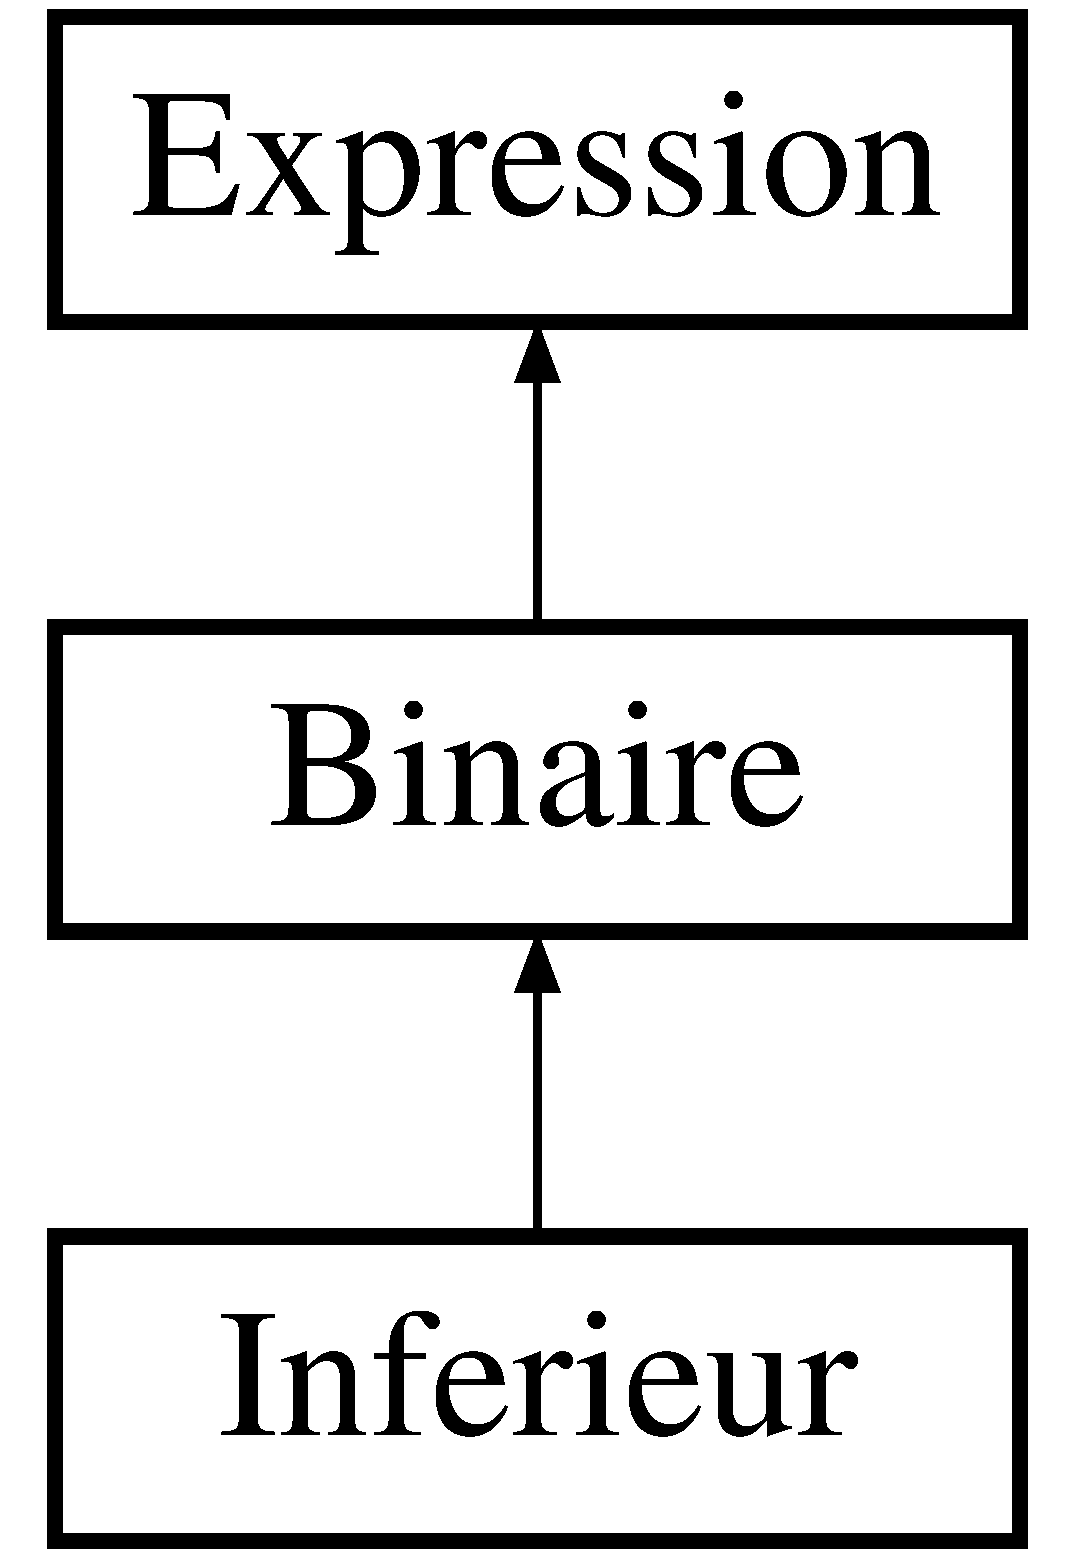
\includegraphics[height=3.000000cm]{class_inferieur}
\end{center}
\end{figure}
\subsection*{Public Member Functions}
\begin{DoxyCompactItemize}
\item 
\hyperlink{class_inferieur_ab2956d52a56cedfc1ec738b535884e3a}{Inferieur} ()
\begin{DoxyCompactList}\small\item\em Constructeur. \end{DoxyCompactList}\item 
virtual \hyperlink{class_inferieur_a444511c43415c3c2b16aaa2551c85e9f}{$\sim$\+Inferieur} ()
\begin{DoxyCompactList}\small\item\em Destructeur Destructeur de la classe \hyperlink{class_inferieur}{Inferieur}. \end{DoxyCompactList}\item 
double \hyperlink{class_inferieur_a8b4e8f22ab48859ad781f1997b083d46}{eval} () const 
\begin{DoxyCompactList}\small\item\em Evalue l\textquotesingle{}expression Methode qui permet d\textquotesingle{}evaluer l\textquotesingle{}expression. \end{DoxyCompactList}\item 
\hyperlink{class_expression}{Expression} $\ast$ \hyperlink{class_inferieur_a40bd4ec1d76deef074b97c6f0959606f}{deriver} (const string \&)
\begin{DoxyCompactList}\small\item\em Derive l\textquotesingle{}expression$\ast$ Methode qui permet deriver l\textquotesingle{}expression. \end{DoxyCompactList}\item 
\hyperlink{class_expression}{Expression} $\ast$ \hyperlink{class_inferieur_a08e1dcb1007cdff4e5fc9303da1df1f3}{simplifier} ()
\begin{DoxyCompactList}\small\item\em Simplifie l\textquotesingle{}expression Methode qui permet de simplifier l\textquotesingle{}expression. \end{DoxyCompactList}\item 
\hyperlink{class_expression}{Expression} $\ast$ \hyperlink{class_inferieur_afdf1b8ba0a235bc1329923ac0fe61fbb}{clone} () const 
\begin{DoxyCompactList}\small\item\em clone l\textquotesingle{}expression Methode qui permet de cloner l\textquotesingle{}expression \end{DoxyCompactList}\item 
string \hyperlink{class_inferieur_ad826ba17b77bdb74d07cab07db30c472}{afficher} () const 
\begin{DoxyCompactList}\small\item\em Affiche l\textquotesingle{}expression Methode qui permet d\textquotesingle{}afficher l\textquotesingle{}expression. \end{DoxyCompactList}\item 
\hyperlink{class_inferieur_aa54c9073af61c06aff7e56e558c2fe96}{Inferieur} (\hyperlink{class_expression}{Expression} $\ast$, \hyperlink{class_expression}{Expression} $\ast$)
\begin{DoxyCompactList}\small\item\em Constructeur. \end{DoxyCompactList}\end{DoxyCompactItemize}
\subsection*{Friends}
\begin{DoxyCompactItemize}
\item 
ostream \& \hyperlink{class_inferieur_a287611af1edf7544ec14a396840cff2c}{operator$<$$<$} (ostream \&, const \hyperlink{class_inferieur}{Inferieur} \&)
\begin{DoxyCompactList}\small\item\em operator$<$$<$ Methode qui permet d\textquotesingle{}afficher l\textquotesingle{}expression \end{DoxyCompactList}\end{DoxyCompactItemize}
\subsection*{Additional Inherited Members}


\subsection{Detailed Description}
La classe \hyperlink{class_inferieur}{Inferieur}. 

Cette classe repr�sente les op�rateurs de comparaison strictement inferieur 

\subsection{Constructor \& Destructor Documentation}
\index{Inferieur@{Inferieur}!Inferieur@{Inferieur}}
\index{Inferieur@{Inferieur}!Inferieur@{Inferieur}}
\subsubsection[{\texorpdfstring{Inferieur()}{Inferieur()}}]{\setlength{\rightskip}{0pt plus 5cm}Inferieur\+::\+Inferieur (
\begin{DoxyParamCaption}
{}
\end{DoxyParamCaption}
)}\hypertarget{class_inferieur_ab2956d52a56cedfc1ec738b535884e3a}{}\label{class_inferieur_ab2956d52a56cedfc1ec738b535884e3a}


Constructeur. 

Constructeur de la classe \hyperlink{class_inferieur}{Inferieur} \index{Inferieur@{Inferieur}!````~Inferieur@{$\sim$\+Inferieur}}
\index{````~Inferieur@{$\sim$\+Inferieur}!Inferieur@{Inferieur}}
\subsubsection[{\texorpdfstring{$\sim$\+Inferieur()}{~Inferieur()}}]{\setlength{\rightskip}{0pt plus 5cm}Inferieur\+::$\sim$\+Inferieur (
\begin{DoxyParamCaption}
{}
\end{DoxyParamCaption}
)\hspace{0.3cm}{\ttfamily [virtual]}}\hypertarget{class_inferieur_a444511c43415c3c2b16aaa2551c85e9f}{}\label{class_inferieur_a444511c43415c3c2b16aaa2551c85e9f}


Destructeur Destructeur de la classe \hyperlink{class_inferieur}{Inferieur}. 

\index{Inferieur@{Inferieur}!Inferieur@{Inferieur}}
\index{Inferieur@{Inferieur}!Inferieur@{Inferieur}}
\subsubsection[{\texorpdfstring{Inferieur(\+Expression $\ast$, Expression $\ast$)}{Inferieur(Expression *, Expression *)}}]{\setlength{\rightskip}{0pt plus 5cm}Inferieur\+::\+Inferieur (
\begin{DoxyParamCaption}
\item[{{\bf Expression} $\ast$}]{exp1, }
\item[{{\bf Expression} $\ast$}]{exp2}
\end{DoxyParamCaption}
)}\hypertarget{class_inferieur_aa54c9073af61c06aff7e56e558c2fe96}{}\label{class_inferieur_aa54c9073af61c06aff7e56e558c2fe96}


Constructeur. 

Constructeur de la classe \hyperlink{class_inferieur}{Inferieur}


\begin{DoxyParams}{Parameters}
{\em exp1} & \+: op�rande gauche \\
\hline
{\em exp2} & \+: op�rande droite \\
\hline
\end{DoxyParams}


\subsection{Member Function Documentation}
\index{Inferieur@{Inferieur}!afficher@{afficher}}
\index{afficher@{afficher}!Inferieur@{Inferieur}}
\subsubsection[{\texorpdfstring{afficher() const }{afficher() const }}]{\setlength{\rightskip}{0pt plus 5cm}string Inferieur\+::afficher (
\begin{DoxyParamCaption}
{}
\end{DoxyParamCaption}
) const\hspace{0.3cm}{\ttfamily [virtual]}}\hypertarget{class_inferieur_ad826ba17b77bdb74d07cab07db30c472}{}\label{class_inferieur_ad826ba17b77bdb74d07cab07db30c472}


Affiche l\textquotesingle{}expression Methode qui permet d\textquotesingle{}afficher l\textquotesingle{}expression. 

\begin{DoxyReturn}{Returns}
Le string d\textquotesingle{}expression 
\end{DoxyReturn}


Reimplemented from \hyperlink{class_expression_a953c7de0302331023987a2fff895cb85}{Expression}.

\index{Inferieur@{Inferieur}!clone@{clone}}
\index{clone@{clone}!Inferieur@{Inferieur}}
\subsubsection[{\texorpdfstring{clone() const }{clone() const }}]{\setlength{\rightskip}{0pt plus 5cm}{\bf Expression} $\ast$ Inferieur\+::clone (
\begin{DoxyParamCaption}
{}
\end{DoxyParamCaption}
) const\hspace{0.3cm}{\ttfamily [virtual]}}\hypertarget{class_inferieur_afdf1b8ba0a235bc1329923ac0fe61fbb}{}\label{class_inferieur_afdf1b8ba0a235bc1329923ac0fe61fbb}


clone l\textquotesingle{}expression Methode qui permet de cloner l\textquotesingle{}expression 

\begin{DoxyReturn}{Returns}
L\textquotesingle{}expression clon� 
\end{DoxyReturn}


Implements \hyperlink{class_expression_ac9fcea09ddd3a650a92c3606118abfb6}{Expression}.

\index{Inferieur@{Inferieur}!deriver@{deriver}}
\index{deriver@{deriver}!Inferieur@{Inferieur}}
\subsubsection[{\texorpdfstring{deriver(const string \&)}{deriver(const string &)}}]{\setlength{\rightskip}{0pt plus 5cm}{\bf Expression} $\ast$ Inferieur\+::deriver (
\begin{DoxyParamCaption}
\item[{const string \&}]{var}
\end{DoxyParamCaption}
)\hspace{0.3cm}{\ttfamily [virtual]}}\hypertarget{class_inferieur_a40bd4ec1d76deef074b97c6f0959606f}{}\label{class_inferieur_a40bd4ec1d76deef074b97c6f0959606f}


Derive l\textquotesingle{}expression$\ast$ Methode qui permet deriver l\textquotesingle{}expression. 

\begin{DoxyReturn}{Returns}
L\textquotesingle{}expression deriv� 
\end{DoxyReturn}


Implements \hyperlink{class_expression_a0a2a2cf2cdb1e8ca556ad59832784193}{Expression}.

\index{Inferieur@{Inferieur}!eval@{eval}}
\index{eval@{eval}!Inferieur@{Inferieur}}
\subsubsection[{\texorpdfstring{eval() const }{eval() const }}]{\setlength{\rightskip}{0pt plus 5cm}double Inferieur\+::eval (
\begin{DoxyParamCaption}
{}
\end{DoxyParamCaption}
) const\hspace{0.3cm}{\ttfamily [virtual]}}\hypertarget{class_inferieur_a8b4e8f22ab48859ad781f1997b083d46}{}\label{class_inferieur_a8b4e8f22ab48859ad781f1997b083d46}


Evalue l\textquotesingle{}expression Methode qui permet d\textquotesingle{}evaluer l\textquotesingle{}expression. 

\begin{DoxyReturn}{Returns}
Le valeur d\textquotesingle{}expression 
\end{DoxyReturn}


Implements \hyperlink{class_expression_a5481c36265e11eff513df87bbc5a1d33}{Expression}.

\index{Inferieur@{Inferieur}!simplifier@{simplifier}}
\index{simplifier@{simplifier}!Inferieur@{Inferieur}}
\subsubsection[{\texorpdfstring{simplifier()}{simplifier()}}]{\setlength{\rightskip}{0pt plus 5cm}{\bf Expression} $\ast$ Inferieur\+::simplifier (
\begin{DoxyParamCaption}
{}
\end{DoxyParamCaption}
)\hspace{0.3cm}{\ttfamily [virtual]}}\hypertarget{class_inferieur_a08e1dcb1007cdff4e5fc9303da1df1f3}{}\label{class_inferieur_a08e1dcb1007cdff4e5fc9303da1df1f3}


Simplifie l\textquotesingle{}expression Methode qui permet de simplifier l\textquotesingle{}expression. 

\begin{DoxyReturn}{Returns}
L\textquotesingle{}expression simplifi� 
\end{DoxyReturn}


Implements \hyperlink{class_expression_a319d06d43ead325c835181419061ae0b}{Expression}.



\subsection{Friends And Related Function Documentation}
\index{Inferieur@{Inferieur}!operator$<$$<$@{operator$<$$<$}}
\index{operator$<$$<$@{operator$<$$<$}!Inferieur@{Inferieur}}
\subsubsection[{\texorpdfstring{operator$<$$<$}{operator<<}}]{\setlength{\rightskip}{0pt plus 5cm}ostream\& operator$<$$<$ (
\begin{DoxyParamCaption}
\item[{ostream \&}]{os, }
\item[{const {\bf Inferieur} \&}]{a}
\end{DoxyParamCaption}
)\hspace{0.3cm}{\ttfamily [friend]}}\hypertarget{class_inferieur_a287611af1edf7544ec14a396840cff2c}{}\label{class_inferieur_a287611af1edf7544ec14a396840cff2c}


operator$<$$<$ Methode qui permet d\textquotesingle{}afficher l\textquotesingle{}expression 



The documentation for this class was generated from the following files\+:\begin{DoxyCompactItemize}
\item 
include/\hyperlink{binaire_8h}{binaire.\+h}\item 
src/\hyperlink{binaire_8cpp}{binaire.\+cpp}\end{DoxyCompactItemize}

\hypertarget{class_inferieur_egal}{}\section{Inferieur\+Egal Class Reference}
\label{class_inferieur_egal}\index{Inferieur\+Egal@{Inferieur\+Egal}}


La classe \hyperlink{class_inferieur_egal}{Inferieur\+Egal}.  




{\ttfamily \#include $<$binaire.\+h$>$}

Inheritance diagram for Inferieur\+Egal\+:\begin{figure}[H]
\begin{center}
\leavevmode
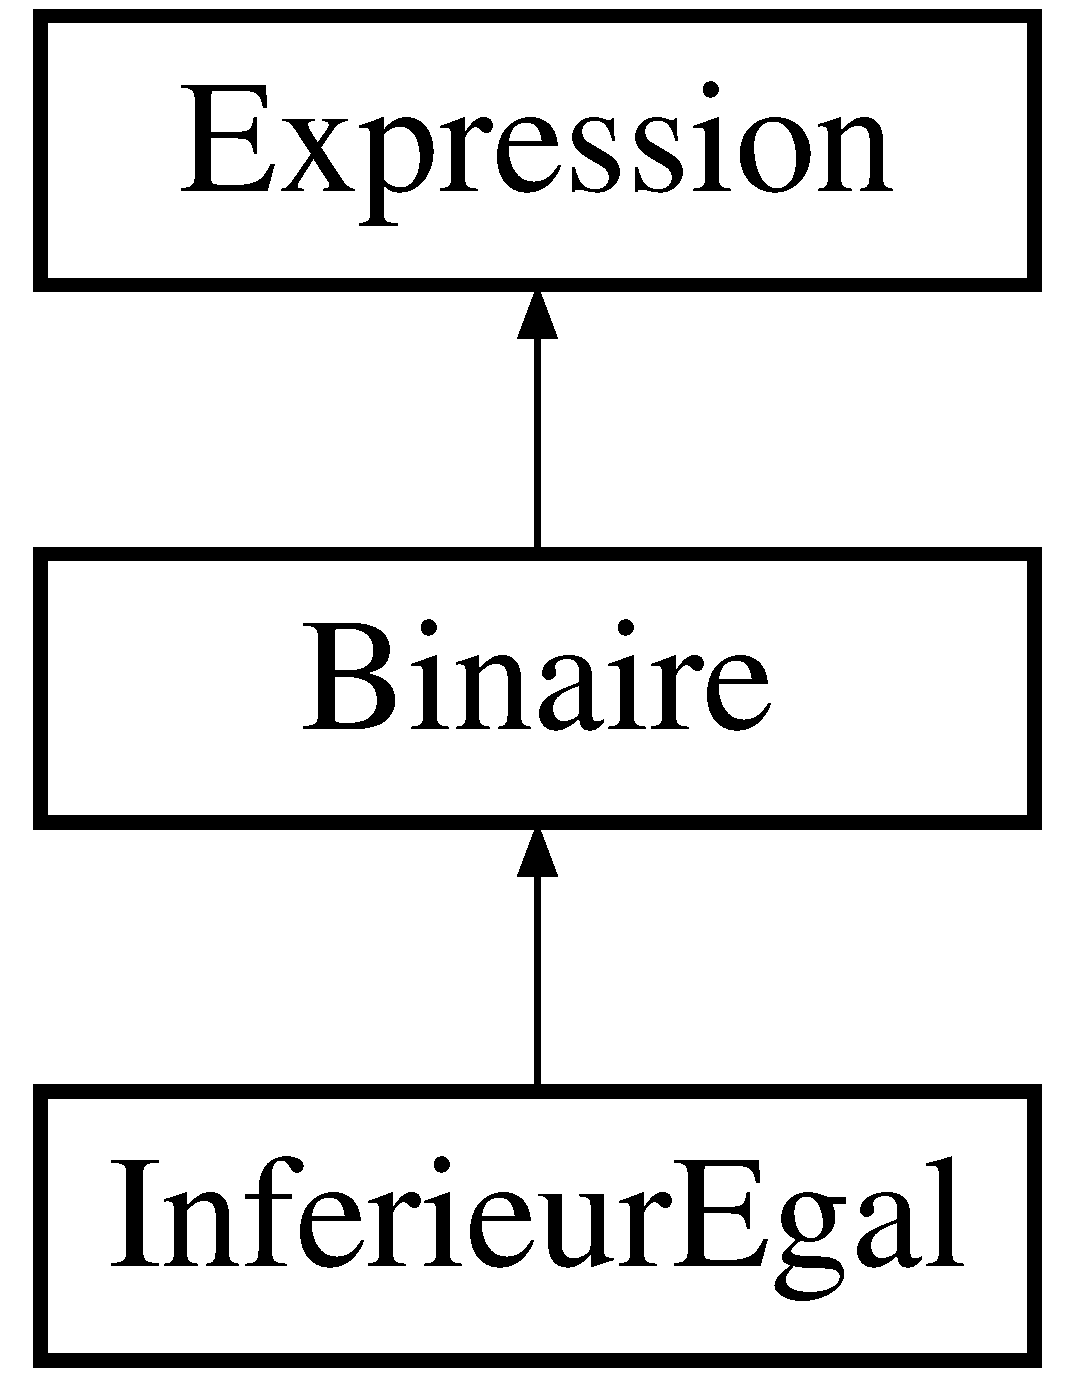
\includegraphics[height=3.000000cm]{class_inferieur_egal}
\end{center}
\end{figure}
\subsection*{Public Member Functions}
\begin{DoxyCompactItemize}
\item 
\hyperlink{class_inferieur_egal_ac913f6039eaa032aa243ca81ce2e17af}{Inferieur\+Egal} ()
\begin{DoxyCompactList}\small\item\em Constructeur. \end{DoxyCompactList}\item 
virtual \hyperlink{class_inferieur_egal_a898d417d29fb7018ad7e6dc9b1ffa495}{$\sim$\+Inferieur\+Egal} ()
\begin{DoxyCompactList}\small\item\em Destructeur Destructeur de la classe \hyperlink{class_inferieur_egal}{Inferieur\+Egal}. \end{DoxyCompactList}\item 
double \hyperlink{class_inferieur_egal_aece49b421f83e80f33eb43adec758cdd}{eval} () const 
\begin{DoxyCompactList}\small\item\em Evalue l\textquotesingle{}expression Methode qui permet d\textquotesingle{}evaluer l\textquotesingle{}expression. \end{DoxyCompactList}\item 
\hyperlink{class_expression}{Expression} $\ast$ \hyperlink{class_inferieur_egal_af3dfc429ad45e2ed60920e423f363e46}{deriver} (const string \&)
\begin{DoxyCompactList}\small\item\em Derive l\textquotesingle{}expression$\ast$ Methode qui permet deriver l\textquotesingle{}expression. \end{DoxyCompactList}\item 
\hyperlink{class_expression}{Expression} $\ast$ \hyperlink{class_inferieur_egal_a65e16573f97d5073fb43c7c91a43e5d3}{simplifier} ()
\begin{DoxyCompactList}\small\item\em Simplifie l\textquotesingle{}expression Methode qui permet de simplifier l\textquotesingle{}expression. \end{DoxyCompactList}\item 
\hyperlink{class_expression}{Expression} $\ast$ \hyperlink{class_inferieur_egal_acdeb552ab7486e0cabe0af7a7e0f4b6c}{clone} () const 
\begin{DoxyCompactList}\small\item\em clone l\textquotesingle{}expression Methode qui permet de cloner l\textquotesingle{}expression \end{DoxyCompactList}\item 
string \hyperlink{class_inferieur_egal_a820821cedaab1a0bce1d13f49c55a006}{afficher} () const 
\begin{DoxyCompactList}\small\item\em Affiche l\textquotesingle{}expression Methode qui permet d\textquotesingle{}afficher l\textquotesingle{}expression. \end{DoxyCompactList}\item 
\hyperlink{class_inferieur_egal_aabff97d23f6e803052dc13584e443bcb}{Inferieur\+Egal} (\hyperlink{class_expression}{Expression} $\ast$, \hyperlink{class_expression}{Expression} $\ast$)
\begin{DoxyCompactList}\small\item\em Constructeur. \end{DoxyCompactList}\end{DoxyCompactItemize}
\subsection*{Friends}
\begin{DoxyCompactItemize}
\item 
ostream \& \hyperlink{class_inferieur_egal_a9d320f32251b9f338f01c9b1c4972f2b}{operator$<$$<$} (ostream \&, const \hyperlink{class_inferieur_egal}{Inferieur\+Egal} \&)
\begin{DoxyCompactList}\small\item\em operator$<$$<$ Methode qui permet d\textquotesingle{}afficher l\textquotesingle{}expression \end{DoxyCompactList}\end{DoxyCompactItemize}
\subsection*{Additional Inherited Members}


\subsection{Detailed Description}
La classe \hyperlink{class_inferieur_egal}{Inferieur\+Egal}. 

Cette classe repr�sente les op�rateurs de comparaison inferieur ou egal 

\subsection{Constructor \& Destructor Documentation}
\index{Inferieur\+Egal@{Inferieur\+Egal}!Inferieur\+Egal@{Inferieur\+Egal}}
\index{Inferieur\+Egal@{Inferieur\+Egal}!Inferieur\+Egal@{Inferieur\+Egal}}
\subsubsection[{\texorpdfstring{Inferieur\+Egal()}{InferieurEgal()}}]{\setlength{\rightskip}{0pt plus 5cm}Inferieur\+Egal\+::\+Inferieur\+Egal (
\begin{DoxyParamCaption}
{}
\end{DoxyParamCaption}
)}\hypertarget{class_inferieur_egal_ac913f6039eaa032aa243ca81ce2e17af}{}\label{class_inferieur_egal_ac913f6039eaa032aa243ca81ce2e17af}


Constructeur. 

Constructeur de la classe \hyperlink{class_inferieur_egal}{Inferieur\+Egal} \index{Inferieur\+Egal@{Inferieur\+Egal}!````~Inferieur\+Egal@{$\sim$\+Inferieur\+Egal}}
\index{````~Inferieur\+Egal@{$\sim$\+Inferieur\+Egal}!Inferieur\+Egal@{Inferieur\+Egal}}
\subsubsection[{\texorpdfstring{$\sim$\+Inferieur\+Egal()}{~InferieurEgal()}}]{\setlength{\rightskip}{0pt plus 5cm}Inferieur\+Egal\+::$\sim$\+Inferieur\+Egal (
\begin{DoxyParamCaption}
{}
\end{DoxyParamCaption}
)\hspace{0.3cm}{\ttfamily [virtual]}}\hypertarget{class_inferieur_egal_a898d417d29fb7018ad7e6dc9b1ffa495}{}\label{class_inferieur_egal_a898d417d29fb7018ad7e6dc9b1ffa495}


Destructeur Destructeur de la classe \hyperlink{class_inferieur_egal}{Inferieur\+Egal}. 

\index{Inferieur\+Egal@{Inferieur\+Egal}!Inferieur\+Egal@{Inferieur\+Egal}}
\index{Inferieur\+Egal@{Inferieur\+Egal}!Inferieur\+Egal@{Inferieur\+Egal}}
\subsubsection[{\texorpdfstring{Inferieur\+Egal(\+Expression $\ast$, Expression $\ast$)}{InferieurEgal(Expression *, Expression *)}}]{\setlength{\rightskip}{0pt plus 5cm}Inferieur\+Egal\+::\+Inferieur\+Egal (
\begin{DoxyParamCaption}
\item[{{\bf Expression} $\ast$}]{exp1, }
\item[{{\bf Expression} $\ast$}]{exp2}
\end{DoxyParamCaption}
)}\hypertarget{class_inferieur_egal_aabff97d23f6e803052dc13584e443bcb}{}\label{class_inferieur_egal_aabff97d23f6e803052dc13584e443bcb}


Constructeur. 

Constructeur de la classe \hyperlink{class_inferieur_egal}{Inferieur\+Egal}


\begin{DoxyParams}{Parameters}
{\em exp1} & \+: op�rande gauche \\
\hline
{\em exp2} & \+: op�rande droite \\
\hline
\end{DoxyParams}


\subsection{Member Function Documentation}
\index{Inferieur\+Egal@{Inferieur\+Egal}!afficher@{afficher}}
\index{afficher@{afficher}!Inferieur\+Egal@{Inferieur\+Egal}}
\subsubsection[{\texorpdfstring{afficher() const }{afficher() const }}]{\setlength{\rightskip}{0pt plus 5cm}string Inferieur\+Egal\+::afficher (
\begin{DoxyParamCaption}
{}
\end{DoxyParamCaption}
) const\hspace{0.3cm}{\ttfamily [virtual]}}\hypertarget{class_inferieur_egal_a820821cedaab1a0bce1d13f49c55a006}{}\label{class_inferieur_egal_a820821cedaab1a0bce1d13f49c55a006}


Affiche l\textquotesingle{}expression Methode qui permet d\textquotesingle{}afficher l\textquotesingle{}expression. 

\begin{DoxyReturn}{Returns}
Le string d\textquotesingle{}expression 
\end{DoxyReturn}


Reimplemented from \hyperlink{class_expression_a953c7de0302331023987a2fff895cb85}{Expression}.

\index{Inferieur\+Egal@{Inferieur\+Egal}!clone@{clone}}
\index{clone@{clone}!Inferieur\+Egal@{Inferieur\+Egal}}
\subsubsection[{\texorpdfstring{clone() const }{clone() const }}]{\setlength{\rightskip}{0pt plus 5cm}{\bf Expression} $\ast$ Inferieur\+Egal\+::clone (
\begin{DoxyParamCaption}
{}
\end{DoxyParamCaption}
) const\hspace{0.3cm}{\ttfamily [virtual]}}\hypertarget{class_inferieur_egal_acdeb552ab7486e0cabe0af7a7e0f4b6c}{}\label{class_inferieur_egal_acdeb552ab7486e0cabe0af7a7e0f4b6c}


clone l\textquotesingle{}expression Methode qui permet de cloner l\textquotesingle{}expression 

\begin{DoxyReturn}{Returns}
L\textquotesingle{}expression clon� 
\end{DoxyReturn}


Implements \hyperlink{class_expression_ac9fcea09ddd3a650a92c3606118abfb6}{Expression}.

\index{Inferieur\+Egal@{Inferieur\+Egal}!deriver@{deriver}}
\index{deriver@{deriver}!Inferieur\+Egal@{Inferieur\+Egal}}
\subsubsection[{\texorpdfstring{deriver(const string \&)}{deriver(const string &)}}]{\setlength{\rightskip}{0pt plus 5cm}{\bf Expression} $\ast$ Inferieur\+Egal\+::deriver (
\begin{DoxyParamCaption}
\item[{const string \&}]{var}
\end{DoxyParamCaption}
)\hspace{0.3cm}{\ttfamily [virtual]}}\hypertarget{class_inferieur_egal_af3dfc429ad45e2ed60920e423f363e46}{}\label{class_inferieur_egal_af3dfc429ad45e2ed60920e423f363e46}


Derive l\textquotesingle{}expression$\ast$ Methode qui permet deriver l\textquotesingle{}expression. 

\begin{DoxyReturn}{Returns}
L\textquotesingle{}expression deriv� 
\end{DoxyReturn}


Implements \hyperlink{class_expression_a0a2a2cf2cdb1e8ca556ad59832784193}{Expression}.

\index{Inferieur\+Egal@{Inferieur\+Egal}!eval@{eval}}
\index{eval@{eval}!Inferieur\+Egal@{Inferieur\+Egal}}
\subsubsection[{\texorpdfstring{eval() const }{eval() const }}]{\setlength{\rightskip}{0pt plus 5cm}double Inferieur\+Egal\+::eval (
\begin{DoxyParamCaption}
{}
\end{DoxyParamCaption}
) const\hspace{0.3cm}{\ttfamily [virtual]}}\hypertarget{class_inferieur_egal_aece49b421f83e80f33eb43adec758cdd}{}\label{class_inferieur_egal_aece49b421f83e80f33eb43adec758cdd}


Evalue l\textquotesingle{}expression Methode qui permet d\textquotesingle{}evaluer l\textquotesingle{}expression. 

\begin{DoxyReturn}{Returns}
Le valeur d\textquotesingle{}expression 
\end{DoxyReturn}


Implements \hyperlink{class_expression_a5481c36265e11eff513df87bbc5a1d33}{Expression}.

\index{Inferieur\+Egal@{Inferieur\+Egal}!simplifier@{simplifier}}
\index{simplifier@{simplifier}!Inferieur\+Egal@{Inferieur\+Egal}}
\subsubsection[{\texorpdfstring{simplifier()}{simplifier()}}]{\setlength{\rightskip}{0pt plus 5cm}{\bf Expression} $\ast$ Inferieur\+Egal\+::simplifier (
\begin{DoxyParamCaption}
{}
\end{DoxyParamCaption}
)\hspace{0.3cm}{\ttfamily [virtual]}}\hypertarget{class_inferieur_egal_a65e16573f97d5073fb43c7c91a43e5d3}{}\label{class_inferieur_egal_a65e16573f97d5073fb43c7c91a43e5d3}


Simplifie l\textquotesingle{}expression Methode qui permet de simplifier l\textquotesingle{}expression. 

\begin{DoxyReturn}{Returns}
L\textquotesingle{}expression simplifi� 
\end{DoxyReturn}


Implements \hyperlink{class_expression_a319d06d43ead325c835181419061ae0b}{Expression}.



\subsection{Friends And Related Function Documentation}
\index{Inferieur\+Egal@{Inferieur\+Egal}!operator$<$$<$@{operator$<$$<$}}
\index{operator$<$$<$@{operator$<$$<$}!Inferieur\+Egal@{Inferieur\+Egal}}
\subsubsection[{\texorpdfstring{operator$<$$<$}{operator<<}}]{\setlength{\rightskip}{0pt plus 5cm}ostream\& operator$<$$<$ (
\begin{DoxyParamCaption}
\item[{ostream \&}]{os, }
\item[{const {\bf Inferieur\+Egal} \&}]{a}
\end{DoxyParamCaption}
)\hspace{0.3cm}{\ttfamily [friend]}}\hypertarget{class_inferieur_egal_a9d320f32251b9f338f01c9b1c4972f2b}{}\label{class_inferieur_egal_a9d320f32251b9f338f01c9b1c4972f2b}


operator$<$$<$ Methode qui permet d\textquotesingle{}afficher l\textquotesingle{}expression 



The documentation for this class was generated from the following files\+:\begin{DoxyCompactItemize}
\item 
include/\hyperlink{binaire_8h}{binaire.\+h}\item 
src/\hyperlink{binaire_8cpp}{binaire.\+cpp}\end{DoxyCompactItemize}

\hypertarget{class_pour}{}\section{Pour Class Reference}
\label{class_pour}\index{Pour@{Pour}}


La classe \hyperlink{class_pour}{Pour}.  




{\ttfamily \#include $<$boucle.\+h$>$}

Inheritance diagram for Pour\+:\begin{figure}[H]
\begin{center}
\leavevmode
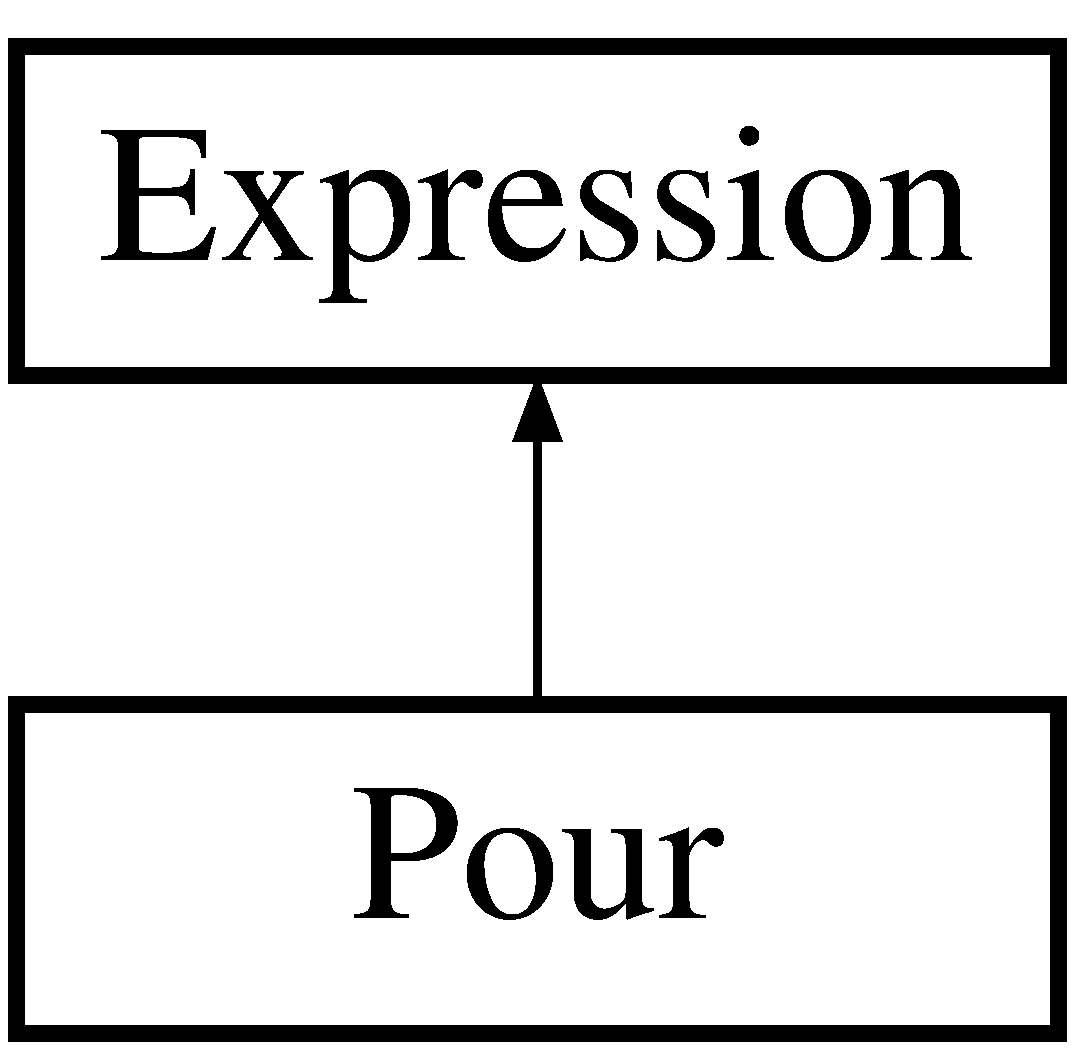
\includegraphics[height=2.000000cm]{class_pour}
\end{center}
\end{figure}
\subsection*{Public Member Functions}
\begin{DoxyCompactItemize}
\item 
\hyperlink{class_pour_a27487d84fcb2c5ceef76a2eea40b2507}{Pour} ()
\begin{DoxyCompactList}\small\item\em Constructeur. \end{DoxyCompactList}\item 
virtual \hyperlink{class_pour_af6e831984dc22ad36dfefede7cee57ca}{$\sim$\+Pour} ()
\begin{DoxyCompactList}\small\item\em Destructeur Destructeur de la classe \hyperlink{class_affectation}{Affectation}. \end{DoxyCompactList}\item 
\hyperlink{class_pour_a03492c109d0097f149b02d493ecc174a}{Pour} (\hyperlink{class_expression}{Expression} $\ast$init, \hyperlink{class_expression}{Expression} $\ast$cond, \hyperlink{class_expression}{Expression} $\ast$inc, \hyperlink{class_expression}{Expression} $\ast$calc)
\begin{DoxyCompactList}\small\item\em Constructeur. \end{DoxyCompactList}\item 
\hyperlink{class_expression}{Expression} $\ast$ \hyperlink{class_pour_a0116d7b9233b8b9dd48999f781f4592f}{clone} () const 
\begin{DoxyCompactList}\small\item\em clone l\textquotesingle{}expression Methode qui permet de cloner l\textquotesingle{}expression \end{DoxyCompactList}\item 
string \hyperlink{class_pour_a7d59b36e80ca85da59c4f5d93ffb674e}{afficher} () const 
\begin{DoxyCompactList}\small\item\em Affiche l\textquotesingle{}expression Methode qui permet d\textquotesingle{}afficher l\textquotesingle{}expression. \end{DoxyCompactList}\item 
double \hyperlink{class_pour_a19f811e4a5d7847cf635f389b09c9e39}{eval} () const 
\begin{DoxyCompactList}\small\item\em Evalue l\textquotesingle{}expression Methode qui permet d\textquotesingle{}evaluer l\textquotesingle{}expression. \end{DoxyCompactList}\item 
\hyperlink{class_expression}{Expression} $\ast$ \hyperlink{class_pour_a6bd2f404e8531dca015c05edced0a63e}{deriver} (const string \&)
\begin{DoxyCompactList}\small\item\em Derive l\textquotesingle{}expression$\ast$ Methode qui permet deriver l\textquotesingle{}expression. \end{DoxyCompactList}\item 
\hyperlink{class_expression}{Expression} $\ast$ \hyperlink{class_pour_a7a03702950b98e370df5fb8ae3ab5417}{simplifier} ()
\begin{DoxyCompactList}\small\item\em Simplifie l\textquotesingle{}expression Methode qui permet de simplifier l\textquotesingle{}expression. \end{DoxyCompactList}\end{DoxyCompactItemize}
\subsection*{Friends}
\begin{DoxyCompactItemize}
\item 
ostream \& \hyperlink{class_pour_a340a834942ee6e157805a6152fce08e9}{operator$<$$<$} (ostream \&os, const \hyperlink{class_pour}{Pour} \&)
\begin{DoxyCompactList}\small\item\em operator$<$$<$ Methode qui permet d\textquotesingle{}afficher l\textquotesingle{}expression \end{DoxyCompactList}\end{DoxyCompactItemize}
\subsection*{Additional Inherited Members}


\subsection{Detailed Description}
La classe \hyperlink{class_pour}{Pour}. 

Cette classe repr�sente les structures it�ratives. Elles permettent de r�aliser des boucles. 

\subsection{Constructor \& Destructor Documentation}
\index{Pour@{Pour}!Pour@{Pour}}
\index{Pour@{Pour}!Pour@{Pour}}
\subsubsection[{\texorpdfstring{Pour()}{Pour()}}]{\setlength{\rightskip}{0pt plus 5cm}Pour\+::\+Pour (
\begin{DoxyParamCaption}
{}
\end{DoxyParamCaption}
)}\hypertarget{class_pour_a27487d84fcb2c5ceef76a2eea40b2507}{}\label{class_pour_a27487d84fcb2c5ceef76a2eea40b2507}


Constructeur. 

Constructeur de la classe \hyperlink{class_pour}{Pour} \index{Pour@{Pour}!````~Pour@{$\sim$\+Pour}}
\index{````~Pour@{$\sim$\+Pour}!Pour@{Pour}}
\subsubsection[{\texorpdfstring{$\sim$\+Pour()}{~Pour()}}]{\setlength{\rightskip}{0pt plus 5cm}Pour\+::$\sim$\+Pour (
\begin{DoxyParamCaption}
{}
\end{DoxyParamCaption}
)\hspace{0.3cm}{\ttfamily [virtual]}}\hypertarget{class_pour_af6e831984dc22ad36dfefede7cee57ca}{}\label{class_pour_af6e831984dc22ad36dfefede7cee57ca}


Destructeur Destructeur de la classe \hyperlink{class_affectation}{Affectation}. 

\index{Pour@{Pour}!Pour@{Pour}}
\index{Pour@{Pour}!Pour@{Pour}}
\subsubsection[{\texorpdfstring{Pour(\+Expression $\ast$init, Expression $\ast$cond, Expression $\ast$inc, Expression $\ast$calc)}{Pour(Expression *init, Expression *cond, Expression *inc, Expression *calc)}}]{\setlength{\rightskip}{0pt plus 5cm}Pour\+::\+Pour (
\begin{DoxyParamCaption}
\item[{{\bf Expression} $\ast$}]{init, }
\item[{{\bf Expression} $\ast$}]{cond, }
\item[{{\bf Expression} $\ast$}]{inc, }
\item[{{\bf Expression} $\ast$}]{calc}
\end{DoxyParamCaption}
)}\hypertarget{class_pour_a03492c109d0097f149b02d493ecc174a}{}\label{class_pour_a03492c109d0097f149b02d493ecc174a}


Constructeur. 

Constructeur de la classe \hyperlink{class_pour}{Pour} 
\begin{DoxyParams}{Parameters}
{\em init} & \+: l\textquotesingle{}initialisation \\
\hline
{\em cond} & \+: le condition \\
\hline
{\em incr} & \+: l\textquotesingle{}incrementaion \\
\hline
{\em calcul} & \+: le calcul \\
\hline
\end{DoxyParams}


\subsection{Member Function Documentation}
\index{Pour@{Pour}!afficher@{afficher}}
\index{afficher@{afficher}!Pour@{Pour}}
\subsubsection[{\texorpdfstring{afficher() const }{afficher() const }}]{\setlength{\rightskip}{0pt plus 5cm}string Pour\+::afficher (
\begin{DoxyParamCaption}
{}
\end{DoxyParamCaption}
) const\hspace{0.3cm}{\ttfamily [virtual]}}\hypertarget{class_pour_a7d59b36e80ca85da59c4f5d93ffb674e}{}\label{class_pour_a7d59b36e80ca85da59c4f5d93ffb674e}


Affiche l\textquotesingle{}expression Methode qui permet d\textquotesingle{}afficher l\textquotesingle{}expression. 

\begin{DoxyReturn}{Returns}
Le string d\textquotesingle{}expression 
\end{DoxyReturn}


Reimplemented from \hyperlink{class_expression_a953c7de0302331023987a2fff895cb85}{Expression}.

\index{Pour@{Pour}!clone@{clone}}
\index{clone@{clone}!Pour@{Pour}}
\subsubsection[{\texorpdfstring{clone() const }{clone() const }}]{\setlength{\rightskip}{0pt plus 5cm}{\bf Expression} $\ast$ Pour\+::clone (
\begin{DoxyParamCaption}
{}
\end{DoxyParamCaption}
) const\hspace{0.3cm}{\ttfamily [virtual]}}\hypertarget{class_pour_a0116d7b9233b8b9dd48999f781f4592f}{}\label{class_pour_a0116d7b9233b8b9dd48999f781f4592f}


clone l\textquotesingle{}expression Methode qui permet de cloner l\textquotesingle{}expression 

\begin{DoxyReturn}{Returns}
L\textquotesingle{}expression clon� 
\end{DoxyReturn}


Implements \hyperlink{class_expression_ac9fcea09ddd3a650a92c3606118abfb6}{Expression}.

\index{Pour@{Pour}!deriver@{deriver}}
\index{deriver@{deriver}!Pour@{Pour}}
\subsubsection[{\texorpdfstring{deriver(const string \&)}{deriver(const string &)}}]{\setlength{\rightskip}{0pt plus 5cm}{\bf Expression} $\ast$ Pour\+::deriver (
\begin{DoxyParamCaption}
\item[{const string \&}]{var}
\end{DoxyParamCaption}
)\hspace{0.3cm}{\ttfamily [virtual]}}\hypertarget{class_pour_a6bd2f404e8531dca015c05edced0a63e}{}\label{class_pour_a6bd2f404e8531dca015c05edced0a63e}


Derive l\textquotesingle{}expression$\ast$ Methode qui permet deriver l\textquotesingle{}expression. 

\begin{DoxyReturn}{Returns}
L\textquotesingle{}expression deriv� 
\end{DoxyReturn}


Implements \hyperlink{class_expression_a0a2a2cf2cdb1e8ca556ad59832784193}{Expression}.

\index{Pour@{Pour}!eval@{eval}}
\index{eval@{eval}!Pour@{Pour}}
\subsubsection[{\texorpdfstring{eval() const }{eval() const }}]{\setlength{\rightskip}{0pt plus 5cm}double Pour\+::eval (
\begin{DoxyParamCaption}
{}
\end{DoxyParamCaption}
) const\hspace{0.3cm}{\ttfamily [virtual]}}\hypertarget{class_pour_a19f811e4a5d7847cf635f389b09c9e39}{}\label{class_pour_a19f811e4a5d7847cf635f389b09c9e39}


Evalue l\textquotesingle{}expression Methode qui permet d\textquotesingle{}evaluer l\textquotesingle{}expression. 

\begin{DoxyReturn}{Returns}
Le valeur d\textquotesingle{}expression 
\end{DoxyReturn}


Implements \hyperlink{class_expression_a5481c36265e11eff513df87bbc5a1d33}{Expression}.

\index{Pour@{Pour}!simplifier@{simplifier}}
\index{simplifier@{simplifier}!Pour@{Pour}}
\subsubsection[{\texorpdfstring{simplifier()}{simplifier()}}]{\setlength{\rightskip}{0pt plus 5cm}{\bf Expression} $\ast$ Pour\+::simplifier (
\begin{DoxyParamCaption}
{}
\end{DoxyParamCaption}
)\hspace{0.3cm}{\ttfamily [virtual]}}\hypertarget{class_pour_a7a03702950b98e370df5fb8ae3ab5417}{}\label{class_pour_a7a03702950b98e370df5fb8ae3ab5417}


Simplifie l\textquotesingle{}expression Methode qui permet de simplifier l\textquotesingle{}expression. 

\begin{DoxyReturn}{Returns}
L\textquotesingle{}expression simplifi� 
\end{DoxyReturn}


Implements \hyperlink{class_expression_a319d06d43ead325c835181419061ae0b}{Expression}.



\subsection{Friends And Related Function Documentation}
\index{Pour@{Pour}!operator$<$$<$@{operator$<$$<$}}
\index{operator$<$$<$@{operator$<$$<$}!Pour@{Pour}}
\subsubsection[{\texorpdfstring{operator$<$$<$}{operator<<}}]{\setlength{\rightskip}{0pt plus 5cm}ostream\& operator$<$$<$ (
\begin{DoxyParamCaption}
\item[{ostream \&}]{os, }
\item[{const {\bf Pour} \&}]{pour}
\end{DoxyParamCaption}
)\hspace{0.3cm}{\ttfamily [friend]}}\hypertarget{class_pour_a340a834942ee6e157805a6152fce08e9}{}\label{class_pour_a340a834942ee6e157805a6152fce08e9}


operator$<$$<$ Methode qui permet d\textquotesingle{}afficher l\textquotesingle{}expression 



The documentation for this class was generated from the following files\+:\begin{DoxyCompactItemize}
\item 
include/\hyperlink{boucle_8h}{boucle.\+h}\item 
src/\hyperlink{boucle_8cpp}{boucle.\+cpp}\end{DoxyCompactItemize}

\hypertarget{class_produit}{}\section{Produit Class Reference}
\label{class_produit}\index{Produit@{Produit}}


La classe \hyperlink{class_produit}{Produit}.  




{\ttfamily \#include $<$binaire.\+h$>$}

Inheritance diagram for Produit\+:\begin{figure}[H]
\begin{center}
\leavevmode
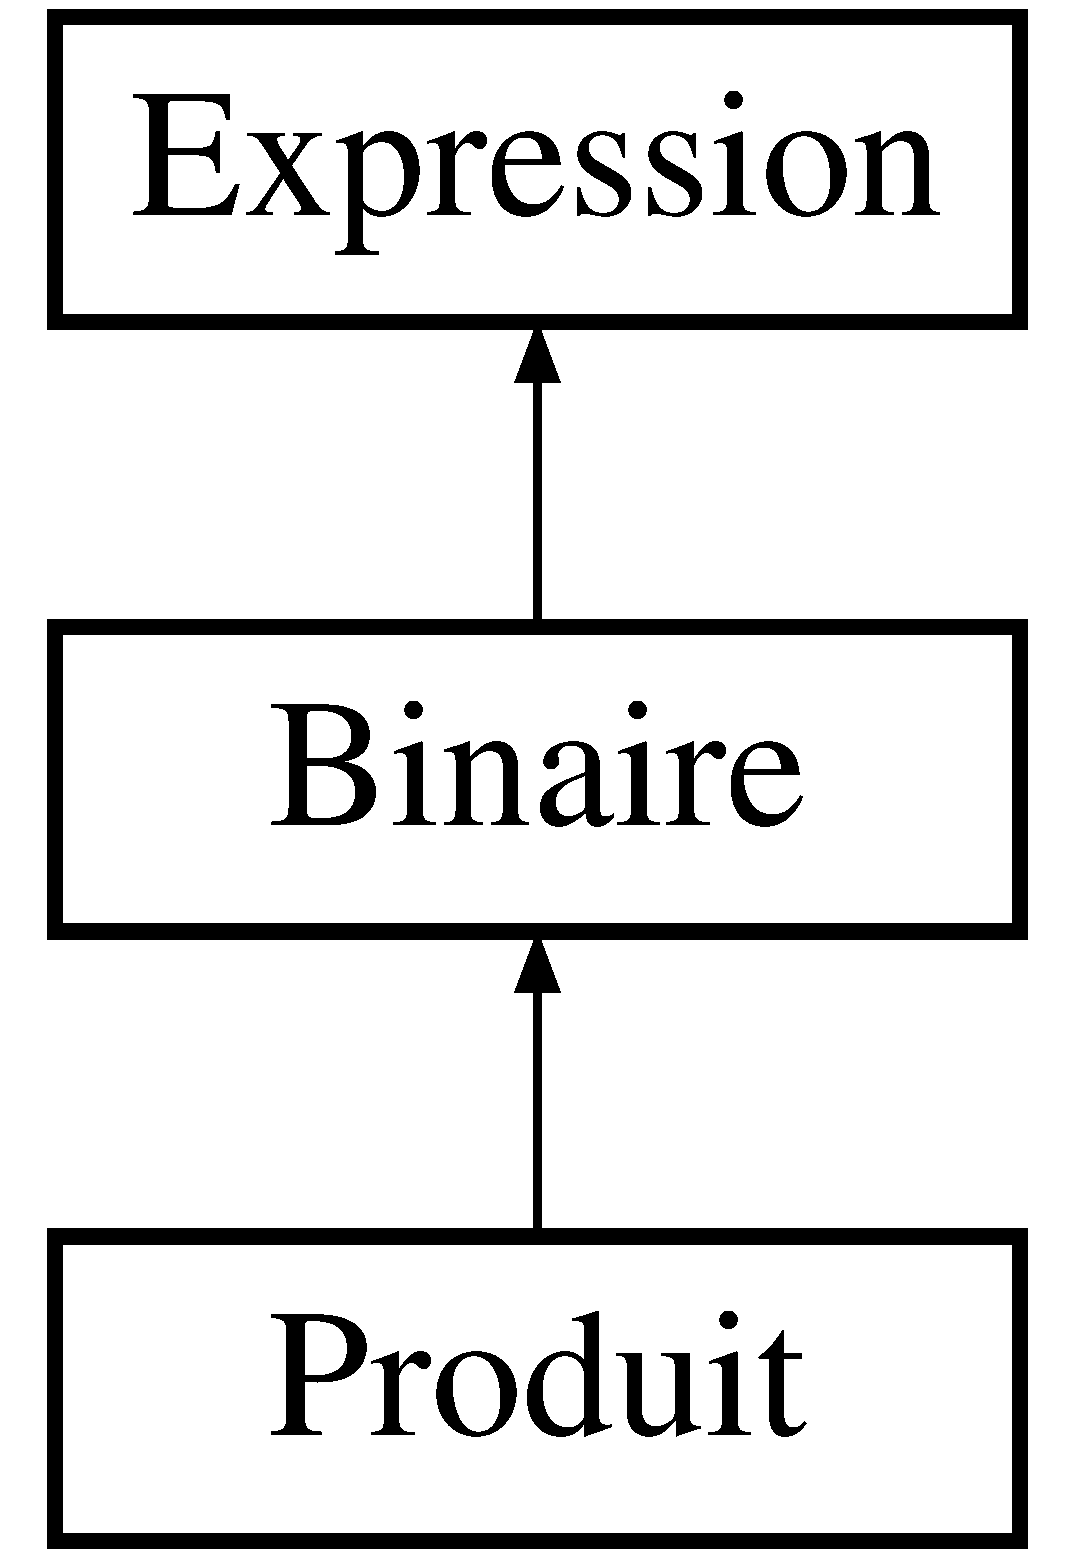
\includegraphics[height=3.000000cm]{class_produit}
\end{center}
\end{figure}
\subsection*{Public Member Functions}
\begin{DoxyCompactItemize}
\item 
\hyperlink{class_produit_af2869859ed8b99b3034ae92db555914b}{Produit} ()
\begin{DoxyCompactList}\small\item\em Constructeur. \end{DoxyCompactList}\item 
virtual \hyperlink{class_produit_a7b789cfa3048436fd050cb565b499c03}{$\sim$\+Produit} ()
\begin{DoxyCompactList}\small\item\em Destructeur Destructeur de la classe \hyperlink{class_produit}{Produit}. \end{DoxyCompactList}\item 
double \hyperlink{class_produit_a6c4efb337679a2cf7ea920c95616d7fe}{eval} () const 
\begin{DoxyCompactList}\small\item\em Evalue l\textquotesingle{}expression Methode qui permet d\textquotesingle{}evaluer l\textquotesingle{}expression. \end{DoxyCompactList}\item 
\hyperlink{class_expression}{Expression} $\ast$ \hyperlink{class_produit_a8aa9088f34b20414cec38451f43f0520}{deriver} (const string \&)
\begin{DoxyCompactList}\small\item\em Derive l\textquotesingle{}expression$\ast$ Methode qui permet deriver l\textquotesingle{}expression. \end{DoxyCompactList}\item 
\hyperlink{class_expression}{Expression} $\ast$ \hyperlink{class_produit_a4b4db95c687fb3d949e67f7b81e9e9ee}{simplifier} ()
\begin{DoxyCompactList}\small\item\em Simplifie l\textquotesingle{}expression Methode qui permet de simplifier l\textquotesingle{}expression. \end{DoxyCompactList}\item 
\hyperlink{class_expression}{Expression} $\ast$ \hyperlink{class_produit_a6fed59a3d22b91d80c59d6fd664c122c}{clone} () const 
\begin{DoxyCompactList}\small\item\em clone l\textquotesingle{}expression Methode qui permet de cloner l\textquotesingle{}expression \end{DoxyCompactList}\item 
string \hyperlink{class_produit_aabe10cf42ec4e382d7b577573bea69a1}{afficher} () const 
\begin{DoxyCompactList}\small\item\em Affiche l\textquotesingle{}expression Methode qui permet d\textquotesingle{}afficher l\textquotesingle{}expression. \end{DoxyCompactList}\item 
\hyperlink{class_produit_a18d03f6a7fb8ef48102cc3f9345b8fc4}{Produit} (\hyperlink{class_expression}{Expression} $\ast$, \hyperlink{class_expression}{Expression} $\ast$, const string \&name=\char`\"{}$\ast$\char`\"{})
\begin{DoxyCompactList}\small\item\em Constructeur. \end{DoxyCompactList}\end{DoxyCompactItemize}
\subsection*{Friends}
\begin{DoxyCompactItemize}
\item 
ostream \& \hyperlink{class_produit_ace0df6a247404de9e4223ac35b2c3024}{operator$<$$<$} (ostream \&, const \hyperlink{class_produit}{Produit} \&)
\begin{DoxyCompactList}\small\item\em operator$<$$<$ Methode qui permet d\textquotesingle{}afficher l\textquotesingle{}expression \end{DoxyCompactList}\end{DoxyCompactItemize}
\subsection*{Additional Inherited Members}


\subsection{Detailed Description}
La classe \hyperlink{class_produit}{Produit}. 

Cette classe repr�sente le multiplication 

\subsection{Constructor \& Destructor Documentation}
\index{Produit@{Produit}!Produit@{Produit}}
\index{Produit@{Produit}!Produit@{Produit}}
\subsubsection[{\texorpdfstring{Produit()}{Produit()}}]{\setlength{\rightskip}{0pt plus 5cm}Produit\+::\+Produit (
\begin{DoxyParamCaption}
{}
\end{DoxyParamCaption}
)}\hypertarget{class_produit_af2869859ed8b99b3034ae92db555914b}{}\label{class_produit_af2869859ed8b99b3034ae92db555914b}


Constructeur. 

Constructeur de la classe \hyperlink{class_produit}{Produit} \index{Produit@{Produit}!````~Produit@{$\sim$\+Produit}}
\index{````~Produit@{$\sim$\+Produit}!Produit@{Produit}}
\subsubsection[{\texorpdfstring{$\sim$\+Produit()}{~Produit()}}]{\setlength{\rightskip}{0pt plus 5cm}Produit\+::$\sim$\+Produit (
\begin{DoxyParamCaption}
{}
\end{DoxyParamCaption}
)\hspace{0.3cm}{\ttfamily [virtual]}}\hypertarget{class_produit_a7b789cfa3048436fd050cb565b499c03}{}\label{class_produit_a7b789cfa3048436fd050cb565b499c03}


Destructeur Destructeur de la classe \hyperlink{class_produit}{Produit}. 

\index{Produit@{Produit}!Produit@{Produit}}
\index{Produit@{Produit}!Produit@{Produit}}
\subsubsection[{\texorpdfstring{Produit(\+Expression $\ast$, Expression $\ast$, const string \&name=""$\ast$"")}{Produit(Expression *, Expression *, const string &name="*")}}]{\setlength{\rightskip}{0pt plus 5cm}Produit\+::\+Produit (
\begin{DoxyParamCaption}
\item[{{\bf Expression} $\ast$}]{exp1, }
\item[{{\bf Expression} $\ast$}]{exp2, }
\item[{const string \&}]{name = {\ttfamily \char`\"{}$\ast$\char`\"{}}}
\end{DoxyParamCaption}
)}\hypertarget{class_produit_a18d03f6a7fb8ef48102cc3f9345b8fc4}{}\label{class_produit_a18d03f6a7fb8ef48102cc3f9345b8fc4}


Constructeur. 

Constructeur de la classe \hyperlink{class_produit}{Produit}


\begin{DoxyParams}{Parameters}
{\em exp1} & \+: op�rande gauche \\
\hline
{\em exp2} & \+: op�rande droite \\
\hline
{\em nom} & \+: nom d\textquotesingle{}expression \\
\hline
\end{DoxyParams}


\subsection{Member Function Documentation}
\index{Produit@{Produit}!afficher@{afficher}}
\index{afficher@{afficher}!Produit@{Produit}}
\subsubsection[{\texorpdfstring{afficher() const }{afficher() const }}]{\setlength{\rightskip}{0pt plus 5cm}string Produit\+::afficher (
\begin{DoxyParamCaption}
{}
\end{DoxyParamCaption}
) const\hspace{0.3cm}{\ttfamily [virtual]}}\hypertarget{class_produit_aabe10cf42ec4e382d7b577573bea69a1}{}\label{class_produit_aabe10cf42ec4e382d7b577573bea69a1}


Affiche l\textquotesingle{}expression Methode qui permet d\textquotesingle{}afficher l\textquotesingle{}expression. 

\begin{DoxyReturn}{Returns}
Le string d\textquotesingle{}expression 
\end{DoxyReturn}


Reimplemented from \hyperlink{class_expression_a953c7de0302331023987a2fff895cb85}{Expression}.

\index{Produit@{Produit}!clone@{clone}}
\index{clone@{clone}!Produit@{Produit}}
\subsubsection[{\texorpdfstring{clone() const }{clone() const }}]{\setlength{\rightskip}{0pt plus 5cm}{\bf Expression} $\ast$ Produit\+::clone (
\begin{DoxyParamCaption}
{}
\end{DoxyParamCaption}
) const\hspace{0.3cm}{\ttfamily [virtual]}}\hypertarget{class_produit_a6fed59a3d22b91d80c59d6fd664c122c}{}\label{class_produit_a6fed59a3d22b91d80c59d6fd664c122c}


clone l\textquotesingle{}expression Methode qui permet de cloner l\textquotesingle{}expression 

\begin{DoxyReturn}{Returns}
L\textquotesingle{}expression clon� 
\end{DoxyReturn}


Implements \hyperlink{class_expression_ac9fcea09ddd3a650a92c3606118abfb6}{Expression}.

\index{Produit@{Produit}!deriver@{deriver}}
\index{deriver@{deriver}!Produit@{Produit}}
\subsubsection[{\texorpdfstring{deriver(const string \&)}{deriver(const string &)}}]{\setlength{\rightskip}{0pt plus 5cm}{\bf Expression} $\ast$ Produit\+::deriver (
\begin{DoxyParamCaption}
\item[{const string \&}]{var}
\end{DoxyParamCaption}
)\hspace{0.3cm}{\ttfamily [virtual]}}\hypertarget{class_produit_a8aa9088f34b20414cec38451f43f0520}{}\label{class_produit_a8aa9088f34b20414cec38451f43f0520}


Derive l\textquotesingle{}expression$\ast$ Methode qui permet deriver l\textquotesingle{}expression. 

\begin{DoxyReturn}{Returns}
L\textquotesingle{}expression deriv� 
\end{DoxyReturn}


Implements \hyperlink{class_expression_a0a2a2cf2cdb1e8ca556ad59832784193}{Expression}.

\index{Produit@{Produit}!eval@{eval}}
\index{eval@{eval}!Produit@{Produit}}
\subsubsection[{\texorpdfstring{eval() const }{eval() const }}]{\setlength{\rightskip}{0pt plus 5cm}double Produit\+::eval (
\begin{DoxyParamCaption}
{}
\end{DoxyParamCaption}
) const\hspace{0.3cm}{\ttfamily [virtual]}}\hypertarget{class_produit_a6c4efb337679a2cf7ea920c95616d7fe}{}\label{class_produit_a6c4efb337679a2cf7ea920c95616d7fe}


Evalue l\textquotesingle{}expression Methode qui permet d\textquotesingle{}evaluer l\textquotesingle{}expression. 

\begin{DoxyReturn}{Returns}
Le valeur d\textquotesingle{}expression 
\end{DoxyReturn}


Implements \hyperlink{class_expression_a5481c36265e11eff513df87bbc5a1d33}{Expression}.

\index{Produit@{Produit}!simplifier@{simplifier}}
\index{simplifier@{simplifier}!Produit@{Produit}}
\subsubsection[{\texorpdfstring{simplifier()}{simplifier()}}]{\setlength{\rightskip}{0pt plus 5cm}{\bf Expression} $\ast$ Produit\+::simplifier (
\begin{DoxyParamCaption}
{}
\end{DoxyParamCaption}
)\hspace{0.3cm}{\ttfamily [virtual]}}\hypertarget{class_produit_a4b4db95c687fb3d949e67f7b81e9e9ee}{}\label{class_produit_a4b4db95c687fb3d949e67f7b81e9e9ee}


Simplifie l\textquotesingle{}expression Methode qui permet de simplifier l\textquotesingle{}expression. 

\begin{DoxyReturn}{Returns}
L\textquotesingle{}expression simplifi� 
\end{DoxyReturn}


Implements \hyperlink{class_expression_a319d06d43ead325c835181419061ae0b}{Expression}.



\subsection{Friends And Related Function Documentation}
\index{Produit@{Produit}!operator$<$$<$@{operator$<$$<$}}
\index{operator$<$$<$@{operator$<$$<$}!Produit@{Produit}}
\subsubsection[{\texorpdfstring{operator$<$$<$}{operator<<}}]{\setlength{\rightskip}{0pt plus 5cm}ostream\& operator$<$$<$ (
\begin{DoxyParamCaption}
\item[{ostream \&}]{os, }
\item[{const {\bf Produit} \&}]{a}
\end{DoxyParamCaption}
)\hspace{0.3cm}{\ttfamily [friend]}}\hypertarget{class_produit_ace0df6a247404de9e4223ac35b2c3024}{}\label{class_produit_ace0df6a247404de9e4223ac35b2c3024}


operator$<$$<$ Methode qui permet d\textquotesingle{}afficher l\textquotesingle{}expression 



The documentation for this class was generated from the following files\+:\begin{DoxyCompactItemize}
\item 
include/\hyperlink{binaire_8h}{binaire.\+h}\item 
src/\hyperlink{binaire_8cpp}{binaire.\+cpp}\end{DoxyCompactItemize}

\hypertarget{class_sin}{}\section{Sin Class Reference}
\label{class_sin}\index{Sin@{Sin}}


La classe \hyperlink{class_sin}{Sin}.  




{\ttfamily \#include $<$unaire.\+h$>$}

Inheritance diagram for Sin\+:\begin{figure}[H]
\begin{center}
\leavevmode
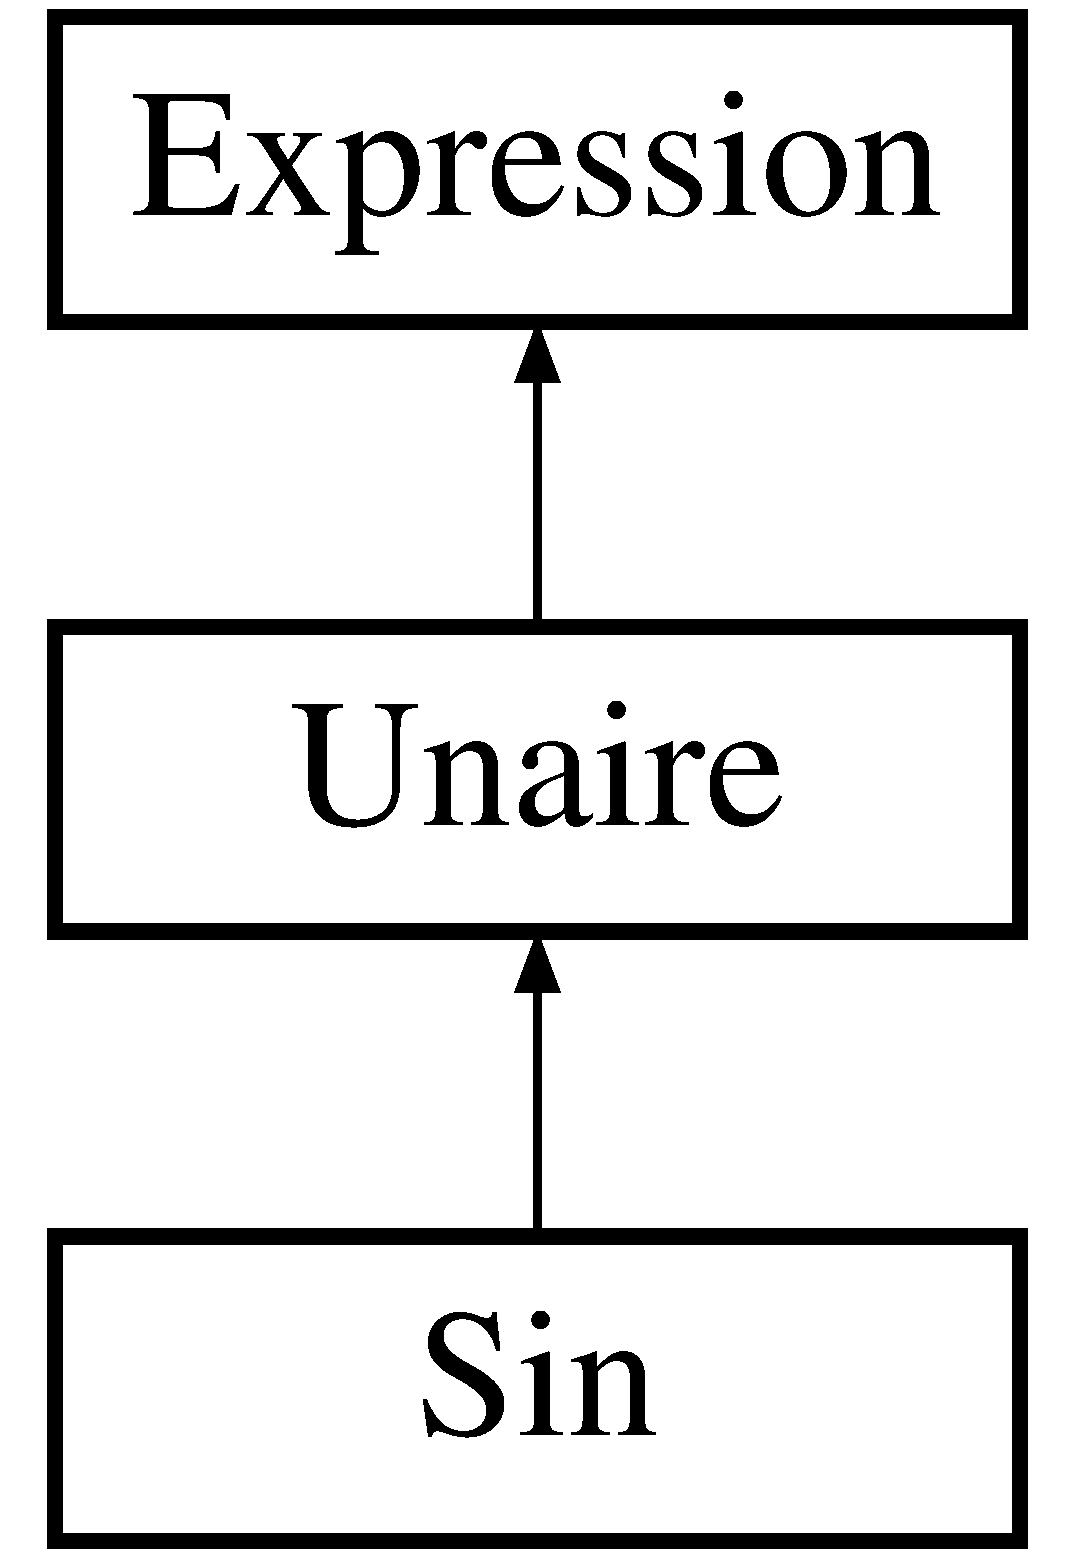
\includegraphics[height=3.000000cm]{class_sin}
\end{center}
\end{figure}
\subsection*{Public Member Functions}
\begin{DoxyCompactItemize}
\item 
\hyperlink{class_sin_ae1f86757154337ee08d5c08033bc2b31}{Sin} ()
\begin{DoxyCompactList}\small\item\em Constructeur. \end{DoxyCompactList}\item 
\hyperlink{class_sin_a36e34f9ef381e6c39426c939360a1b00}{Sin} (\hyperlink{class_expression}{Expression} $\ast$, const string \&name=\char`\"{}sin\char`\"{})
\begin{DoxyCompactList}\small\item\em Constructeur. \end{DoxyCompactList}\item 
virtual \hyperlink{class_sin_a92abdb2b382b852a71115f2d12b03fdf}{$\sim$\+Sin} ()
\begin{DoxyCompactList}\small\item\em Destructeur Destructeur de la classe \hyperlink{class_affectation}{Affectation}. \end{DoxyCompactList}\item 
\hyperlink{class_expression}{Expression} $\ast$ \hyperlink{class_sin_a12ca12d6edd6a6d98566b1befef978c4}{clone} () const 
\begin{DoxyCompactList}\small\item\em clone l\textquotesingle{}expression Methode qui permet de cloner l\textquotesingle{}expression \end{DoxyCompactList}\item 
double \hyperlink{class_sin_a12366e0380d5f03f5a83b09a6b861b35}{eval} () const 
\begin{DoxyCompactList}\small\item\em Evalue l\textquotesingle{}expression Methode qui permet d\textquotesingle{}evaluer l\textquotesingle{}expression. \end{DoxyCompactList}\item 
\hyperlink{class_expression}{Expression} $\ast$ \hyperlink{class_sin_a62c81e668f29b126f7fcc6ed4e6fb4dc}{deriver} (const string \&)
\begin{DoxyCompactList}\small\item\em Derive l\textquotesingle{}expression$\ast$ Methode qui permet deriver l\textquotesingle{}expression. \end{DoxyCompactList}\item 
\hyperlink{class_expression}{Expression} $\ast$ \hyperlink{class_sin_aa988c5b6f05d2452975ed35125b4fa08}{simplifier} ()
\begin{DoxyCompactList}\small\item\em Simplifie l\textquotesingle{}expression Methode qui permet de simplifier l\textquotesingle{}expression. \end{DoxyCompactList}\end{DoxyCompactItemize}
\subsection*{Protected Attributes}
\begin{DoxyCompactItemize}
\item 
double \hyperlink{class_sin_aeb1bec4f4e8d0f65ca9925af6b3e05bc}{val}
\end{DoxyCompactItemize}
\subsection*{Additional Inherited Members}


\subsection{Detailed Description}
La classe \hyperlink{class_sin}{Sin}. 

Cette classe repr�sente le \hyperlink{class_sin}{Sin}. 

\subsection{Constructor \& Destructor Documentation}
\index{Sin@{Sin}!Sin@{Sin}}
\index{Sin@{Sin}!Sin@{Sin}}
\subsubsection[{\texorpdfstring{Sin()}{Sin()}}]{\setlength{\rightskip}{0pt plus 5cm}Sin\+::\+Sin (
\begin{DoxyParamCaption}
{}
\end{DoxyParamCaption}
)}\hypertarget{class_sin_ae1f86757154337ee08d5c08033bc2b31}{}\label{class_sin_ae1f86757154337ee08d5c08033bc2b31}


Constructeur. 

Constructeur de la classe \hyperlink{class_sin}{Sin} \index{Sin@{Sin}!Sin@{Sin}}
\index{Sin@{Sin}!Sin@{Sin}}
\subsubsection[{\texorpdfstring{Sin(\+Expression $\ast$, const string \&name=""sin"")}{Sin(Expression *, const string &name="sin")}}]{\setlength{\rightskip}{0pt plus 5cm}Sin\+::\+Sin (
\begin{DoxyParamCaption}
\item[{{\bf Expression} $\ast$}]{exp, }
\item[{const string \&}]{name = {\ttfamily \char`\"{}sin\char`\"{}}}
\end{DoxyParamCaption}
)}\hypertarget{class_sin_a36e34f9ef381e6c39426c939360a1b00}{}\label{class_sin_a36e34f9ef381e6c39426c939360a1b00}


Constructeur. 

Constructeur de la classe \hyperlink{class_sin}{Sin}


\begin{DoxyParams}{Parameters}
{\em exp} & \+: l\textquotesingle{}expression \\
\hline
{\em nom} & \+: le nom \\
\hline
\end{DoxyParams}
\index{Sin@{Sin}!````~Sin@{$\sim$\+Sin}}
\index{````~Sin@{$\sim$\+Sin}!Sin@{Sin}}
\subsubsection[{\texorpdfstring{$\sim$\+Sin()}{~Sin()}}]{\setlength{\rightskip}{0pt plus 5cm}Sin\+::$\sim$\+Sin (
\begin{DoxyParamCaption}
{}
\end{DoxyParamCaption}
)\hspace{0.3cm}{\ttfamily [virtual]}}\hypertarget{class_sin_a92abdb2b382b852a71115f2d12b03fdf}{}\label{class_sin_a92abdb2b382b852a71115f2d12b03fdf}


Destructeur Destructeur de la classe \hyperlink{class_affectation}{Affectation}. 



\subsection{Member Function Documentation}
\index{Sin@{Sin}!clone@{clone}}
\index{clone@{clone}!Sin@{Sin}}
\subsubsection[{\texorpdfstring{clone() const }{clone() const }}]{\setlength{\rightskip}{0pt plus 5cm}{\bf Expression} $\ast$ Sin\+::clone (
\begin{DoxyParamCaption}
{}
\end{DoxyParamCaption}
) const\hspace{0.3cm}{\ttfamily [virtual]}}\hypertarget{class_sin_a12ca12d6edd6a6d98566b1befef978c4}{}\label{class_sin_a12ca12d6edd6a6d98566b1befef978c4}


clone l\textquotesingle{}expression Methode qui permet de cloner l\textquotesingle{}expression 

\begin{DoxyReturn}{Returns}
L\textquotesingle{}expression clon� 
\end{DoxyReturn}


Implements \hyperlink{class_expression_ac9fcea09ddd3a650a92c3606118abfb6}{Expression}.

\index{Sin@{Sin}!deriver@{deriver}}
\index{deriver@{deriver}!Sin@{Sin}}
\subsubsection[{\texorpdfstring{deriver(const string \&)}{deriver(const string &)}}]{\setlength{\rightskip}{0pt plus 5cm}{\bf Expression} $\ast$ Sin\+::deriver (
\begin{DoxyParamCaption}
\item[{const string \&}]{var}
\end{DoxyParamCaption}
)\hspace{0.3cm}{\ttfamily [virtual]}}\hypertarget{class_sin_a62c81e668f29b126f7fcc6ed4e6fb4dc}{}\label{class_sin_a62c81e668f29b126f7fcc6ed4e6fb4dc}


Derive l\textquotesingle{}expression$\ast$ Methode qui permet deriver l\textquotesingle{}expression. 

\begin{DoxyReturn}{Returns}
L\textquotesingle{}expression deriv� 
\end{DoxyReturn}


Implements \hyperlink{class_expression_a0a2a2cf2cdb1e8ca556ad59832784193}{Expression}.

\index{Sin@{Sin}!eval@{eval}}
\index{eval@{eval}!Sin@{Sin}}
\subsubsection[{\texorpdfstring{eval() const }{eval() const }}]{\setlength{\rightskip}{0pt plus 5cm}double Sin\+::eval (
\begin{DoxyParamCaption}
{}
\end{DoxyParamCaption}
) const\hspace{0.3cm}{\ttfamily [virtual]}}\hypertarget{class_sin_a12366e0380d5f03f5a83b09a6b861b35}{}\label{class_sin_a12366e0380d5f03f5a83b09a6b861b35}


Evalue l\textquotesingle{}expression Methode qui permet d\textquotesingle{}evaluer l\textquotesingle{}expression. 

\begin{DoxyReturn}{Returns}
Le valeur d\textquotesingle{}expression 
\end{DoxyReturn}


Implements \hyperlink{class_expression_a5481c36265e11eff513df87bbc5a1d33}{Expression}.

\index{Sin@{Sin}!simplifier@{simplifier}}
\index{simplifier@{simplifier}!Sin@{Sin}}
\subsubsection[{\texorpdfstring{simplifier()}{simplifier()}}]{\setlength{\rightskip}{0pt plus 5cm}{\bf Expression} $\ast$ Sin\+::simplifier (
\begin{DoxyParamCaption}
{}
\end{DoxyParamCaption}
)\hspace{0.3cm}{\ttfamily [virtual]}}\hypertarget{class_sin_aa988c5b6f05d2452975ed35125b4fa08}{}\label{class_sin_aa988c5b6f05d2452975ed35125b4fa08}


Simplifie l\textquotesingle{}expression Methode qui permet de simplifier l\textquotesingle{}expression. 

\begin{DoxyReturn}{Returns}
L\textquotesingle{}expression simplifi� 
\end{DoxyReturn}


Implements \hyperlink{class_expression_a319d06d43ead325c835181419061ae0b}{Expression}.



\subsection{Member Data Documentation}
\index{Sin@{Sin}!val@{val}}
\index{val@{val}!Sin@{Sin}}
\subsubsection[{\texorpdfstring{val}{val}}]{\setlength{\rightskip}{0pt plus 5cm}double Sin\+::val\hspace{0.3cm}{\ttfamily [protected]}}\hypertarget{class_sin_aeb1bec4f4e8d0f65ca9925af6b3e05bc}{}\label{class_sin_aeb1bec4f4e8d0f65ca9925af6b3e05bc}


The documentation for this class was generated from the following files\+:\begin{DoxyCompactItemize}
\item 
include/\hyperlink{unaire_8h}{unaire.\+h}\item 
src/\hyperlink{unaire_8cpp}{unaire.\+cpp}\end{DoxyCompactItemize}

\hypertarget{class_somme}{}\section{Somme Class Reference}
\label{class_somme}\index{Somme@{Somme}}


La classe \hyperlink{class_somme}{Somme}.  




{\ttfamily \#include $<$binaire.\+h$>$}

Inheritance diagram for Somme\+:\begin{figure}[H]
\begin{center}
\leavevmode
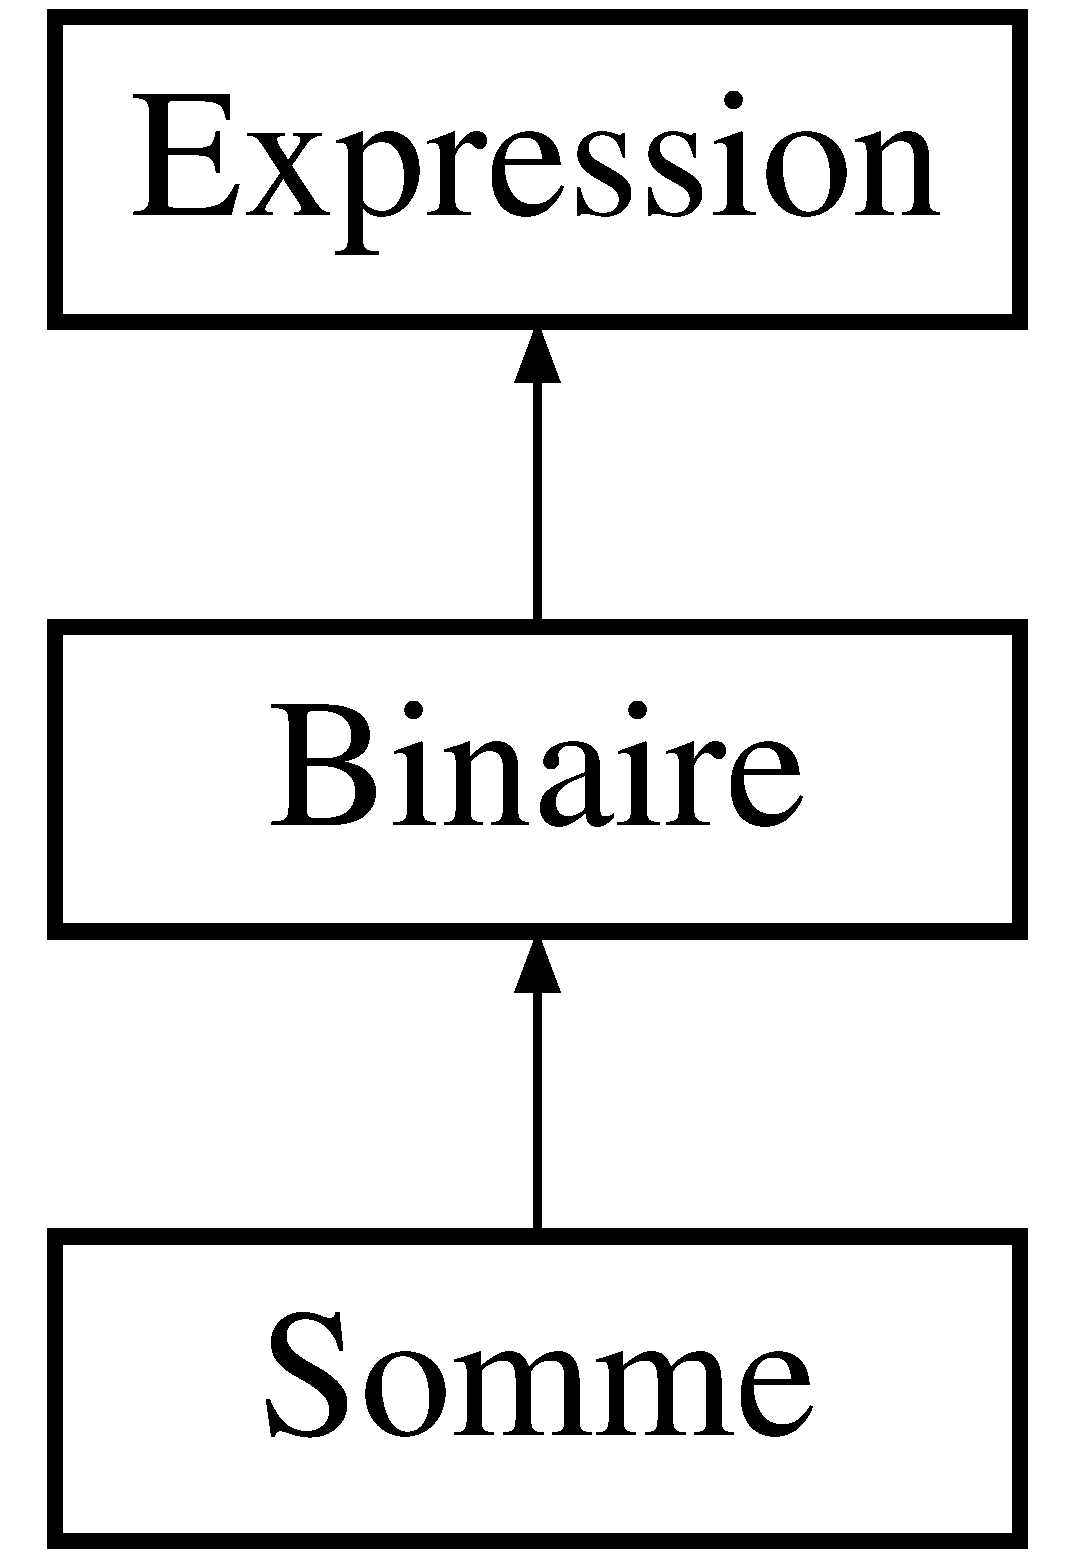
\includegraphics[height=3.000000cm]{class_somme}
\end{center}
\end{figure}
\subsection*{Public Member Functions}
\begin{DoxyCompactItemize}
\item 
\hyperlink{class_somme_a1861adc5929f9fe4de0dd56286658a83}{Somme} ()
\begin{DoxyCompactList}\small\item\em Constructeur. \end{DoxyCompactList}\item 
virtual \hyperlink{class_somme_ab19d1e90427f712aeb8588bfa8c57695}{$\sim$\+Somme} ()
\begin{DoxyCompactList}\small\item\em Destructeur Destructeur de la classe \hyperlink{class_somme}{Somme}. \end{DoxyCompactList}\item 
double \hyperlink{class_somme_ab36403713c60f51ee6eebc5693ce3891}{eval} () const 
\begin{DoxyCompactList}\small\item\em Evalue l\textquotesingle{}expression Methode qui permet d\textquotesingle{}evaluer l\textquotesingle{}expression. \end{DoxyCompactList}\item 
\hyperlink{class_expression}{Expression} $\ast$ \hyperlink{class_somme_a6288da4022b7ee227431e0531ddd4664}{deriver} (const string \&)
\begin{DoxyCompactList}\small\item\em Derive l\textquotesingle{}expression$\ast$ Methode qui permet deriver l\textquotesingle{}expression. \end{DoxyCompactList}\item 
\hyperlink{class_expression}{Expression} $\ast$ \hyperlink{class_somme_a486f0b09a4697593b638486428b849f3}{simplifier} ()
\begin{DoxyCompactList}\small\item\em Simplifie l\textquotesingle{}expression Methode qui permet de simplifier l\textquotesingle{}expression. \end{DoxyCompactList}\item 
\hyperlink{class_expression}{Expression} $\ast$ \hyperlink{class_somme_aaf95e8388a3eb28edddd205805d9c10b}{clone} () const 
\begin{DoxyCompactList}\small\item\em clone l\textquotesingle{}expression Methode qui permet de cloner l\textquotesingle{}expression \end{DoxyCompactList}\item 
string \hyperlink{class_somme_a3605a67027a5d0f7dc8c7617d2b1edfc}{afficher} () const 
\begin{DoxyCompactList}\small\item\em Affiche l\textquotesingle{}expression Methode qui permet d\textquotesingle{}afficher l\textquotesingle{}expression. \end{DoxyCompactList}\item 
\hyperlink{class_somme_ae5906811dbacd97ec59894b21fc1e9e5}{Somme} (\hyperlink{class_expression}{Expression} $\ast$, \hyperlink{class_expression}{Expression} $\ast$, const string \&name=\char`\"{}+\char`\"{})
\begin{DoxyCompactList}\small\item\em Constructeur. \end{DoxyCompactList}\end{DoxyCompactItemize}
\subsection*{Friends}
\begin{DoxyCompactItemize}
\item 
ostream \& \hyperlink{class_somme_a9fcd5c94b0112e235473850eaa8da455}{operator$<$$<$} (ostream \&, const \hyperlink{class_somme}{Somme} \&)
\begin{DoxyCompactList}\small\item\em operator$<$$<$ Methode qui permet d\textquotesingle{}afficher l\textquotesingle{}expression \end{DoxyCompactList}\end{DoxyCompactItemize}
\subsection*{Additional Inherited Members}


\subsection{Detailed Description}
La classe \hyperlink{class_somme}{Somme}. 

Cette classe repr�sente l\textquotesingle{}addition 

\subsection{Constructor \& Destructor Documentation}
\index{Somme@{Somme}!Somme@{Somme}}
\index{Somme@{Somme}!Somme@{Somme}}
\subsubsection[{\texorpdfstring{Somme()}{Somme()}}]{\setlength{\rightskip}{0pt plus 5cm}Somme\+::\+Somme (
\begin{DoxyParamCaption}
{}
\end{DoxyParamCaption}
)}\hypertarget{class_somme_a1861adc5929f9fe4de0dd56286658a83}{}\label{class_somme_a1861adc5929f9fe4de0dd56286658a83}


Constructeur. 

Constructeur de la classe \hyperlink{class_somme}{Somme} \index{Somme@{Somme}!````~Somme@{$\sim$\+Somme}}
\index{````~Somme@{$\sim$\+Somme}!Somme@{Somme}}
\subsubsection[{\texorpdfstring{$\sim$\+Somme()}{~Somme()}}]{\setlength{\rightskip}{0pt plus 5cm}Somme\+::$\sim$\+Somme (
\begin{DoxyParamCaption}
{}
\end{DoxyParamCaption}
)\hspace{0.3cm}{\ttfamily [virtual]}}\hypertarget{class_somme_ab19d1e90427f712aeb8588bfa8c57695}{}\label{class_somme_ab19d1e90427f712aeb8588bfa8c57695}


Destructeur Destructeur de la classe \hyperlink{class_somme}{Somme}. 

\index{Somme@{Somme}!Somme@{Somme}}
\index{Somme@{Somme}!Somme@{Somme}}
\subsubsection[{\texorpdfstring{Somme(\+Expression $\ast$, Expression $\ast$, const string \&name=""+"")}{Somme(Expression *, Expression *, const string &name="+")}}]{\setlength{\rightskip}{0pt plus 5cm}Somme\+::\+Somme (
\begin{DoxyParamCaption}
\item[{{\bf Expression} $\ast$}]{exp1, }
\item[{{\bf Expression} $\ast$}]{exp2, }
\item[{const string \&}]{name = {\ttfamily \char`\"{}+\char`\"{}}}
\end{DoxyParamCaption}
)}\hypertarget{class_somme_ae5906811dbacd97ec59894b21fc1e9e5}{}\label{class_somme_ae5906811dbacd97ec59894b21fc1e9e5}


Constructeur. 

Constructeur de la classe \hyperlink{class_somme}{Somme}


\begin{DoxyParams}{Parameters}
{\em exp1} & \+: op�rande gauche \\
\hline
{\em exp2} & \+: op�rande droite \\
\hline
{\em nom} & \+: nom d\textquotesingle{}expression \\
\hline
\end{DoxyParams}


\subsection{Member Function Documentation}
\index{Somme@{Somme}!afficher@{afficher}}
\index{afficher@{afficher}!Somme@{Somme}}
\subsubsection[{\texorpdfstring{afficher() const }{afficher() const }}]{\setlength{\rightskip}{0pt plus 5cm}string Somme\+::afficher (
\begin{DoxyParamCaption}
{}
\end{DoxyParamCaption}
) const\hspace{0.3cm}{\ttfamily [virtual]}}\hypertarget{class_somme_a3605a67027a5d0f7dc8c7617d2b1edfc}{}\label{class_somme_a3605a67027a5d0f7dc8c7617d2b1edfc}


Affiche l\textquotesingle{}expression Methode qui permet d\textquotesingle{}afficher l\textquotesingle{}expression. 

\begin{DoxyReturn}{Returns}
Le string d\textquotesingle{}expression 
\end{DoxyReturn}


Reimplemented from \hyperlink{class_expression_a953c7de0302331023987a2fff895cb85}{Expression}.

\index{Somme@{Somme}!clone@{clone}}
\index{clone@{clone}!Somme@{Somme}}
\subsubsection[{\texorpdfstring{clone() const }{clone() const }}]{\setlength{\rightskip}{0pt plus 5cm}{\bf Expression} $\ast$ Somme\+::clone (
\begin{DoxyParamCaption}
{}
\end{DoxyParamCaption}
) const\hspace{0.3cm}{\ttfamily [virtual]}}\hypertarget{class_somme_aaf95e8388a3eb28edddd205805d9c10b}{}\label{class_somme_aaf95e8388a3eb28edddd205805d9c10b}


clone l\textquotesingle{}expression Methode qui permet de cloner l\textquotesingle{}expression 

\begin{DoxyReturn}{Returns}
L\textquotesingle{}expression clon� 
\end{DoxyReturn}


Implements \hyperlink{class_expression_ac9fcea09ddd3a650a92c3606118abfb6}{Expression}.

\index{Somme@{Somme}!deriver@{deriver}}
\index{deriver@{deriver}!Somme@{Somme}}
\subsubsection[{\texorpdfstring{deriver(const string \&)}{deriver(const string &)}}]{\setlength{\rightskip}{0pt plus 5cm}{\bf Expression} $\ast$ Somme\+::deriver (
\begin{DoxyParamCaption}
\item[{const string \&}]{var}
\end{DoxyParamCaption}
)\hspace{0.3cm}{\ttfamily [virtual]}}\hypertarget{class_somme_a6288da4022b7ee227431e0531ddd4664}{}\label{class_somme_a6288da4022b7ee227431e0531ddd4664}


Derive l\textquotesingle{}expression$\ast$ Methode qui permet deriver l\textquotesingle{}expression. 

\begin{DoxyReturn}{Returns}
L\textquotesingle{}expression deriv� 
\end{DoxyReturn}


Implements \hyperlink{class_expression_a0a2a2cf2cdb1e8ca556ad59832784193}{Expression}.

\index{Somme@{Somme}!eval@{eval}}
\index{eval@{eval}!Somme@{Somme}}
\subsubsection[{\texorpdfstring{eval() const }{eval() const }}]{\setlength{\rightskip}{0pt plus 5cm}double Somme\+::eval (
\begin{DoxyParamCaption}
{}
\end{DoxyParamCaption}
) const\hspace{0.3cm}{\ttfamily [virtual]}}\hypertarget{class_somme_ab36403713c60f51ee6eebc5693ce3891}{}\label{class_somme_ab36403713c60f51ee6eebc5693ce3891}


Evalue l\textquotesingle{}expression Methode qui permet d\textquotesingle{}evaluer l\textquotesingle{}expression. 

\begin{DoxyReturn}{Returns}
Le valeur d\textquotesingle{}expression 
\end{DoxyReturn}


Implements \hyperlink{class_expression_a5481c36265e11eff513df87bbc5a1d33}{Expression}.

\index{Somme@{Somme}!simplifier@{simplifier}}
\index{simplifier@{simplifier}!Somme@{Somme}}
\subsubsection[{\texorpdfstring{simplifier()}{simplifier()}}]{\setlength{\rightskip}{0pt plus 5cm}{\bf Expression} $\ast$ Somme\+::simplifier (
\begin{DoxyParamCaption}
{}
\end{DoxyParamCaption}
)\hspace{0.3cm}{\ttfamily [virtual]}}\hypertarget{class_somme_a486f0b09a4697593b638486428b849f3}{}\label{class_somme_a486f0b09a4697593b638486428b849f3}


Simplifie l\textquotesingle{}expression Methode qui permet de simplifier l\textquotesingle{}expression. 

\begin{DoxyReturn}{Returns}
L\textquotesingle{}expression simplifi� 
\end{DoxyReturn}


Implements \hyperlink{class_expression_a319d06d43ead325c835181419061ae0b}{Expression}.



\subsection{Friends And Related Function Documentation}
\index{Somme@{Somme}!operator$<$$<$@{operator$<$$<$}}
\index{operator$<$$<$@{operator$<$$<$}!Somme@{Somme}}
\subsubsection[{\texorpdfstring{operator$<$$<$}{operator<<}}]{\setlength{\rightskip}{0pt plus 5cm}ostream\& operator$<$$<$ (
\begin{DoxyParamCaption}
\item[{ostream \&}]{os, }
\item[{const {\bf Somme} \&}]{a}
\end{DoxyParamCaption}
)\hspace{0.3cm}{\ttfamily [friend]}}\hypertarget{class_somme_a9fcd5c94b0112e235473850eaa8da455}{}\label{class_somme_a9fcd5c94b0112e235473850eaa8da455}


operator$<$$<$ Methode qui permet d\textquotesingle{}afficher l\textquotesingle{}expression 



The documentation for this class was generated from the following files\+:\begin{DoxyCompactItemize}
\item 
include/\hyperlink{binaire_8h}{binaire.\+h}\item 
src/\hyperlink{binaire_8cpp}{binaire.\+cpp}\end{DoxyCompactItemize}

\hypertarget{class_superieur}{}\section{Superieur Class Reference}
\label{class_superieur}\index{Superieur@{Superieur}}


La classe \hyperlink{class_superieur}{Superieur}.  




{\ttfamily \#include $<$binaire.\+h$>$}

Inheritance diagram for Superieur\+:\begin{figure}[H]
\begin{center}
\leavevmode
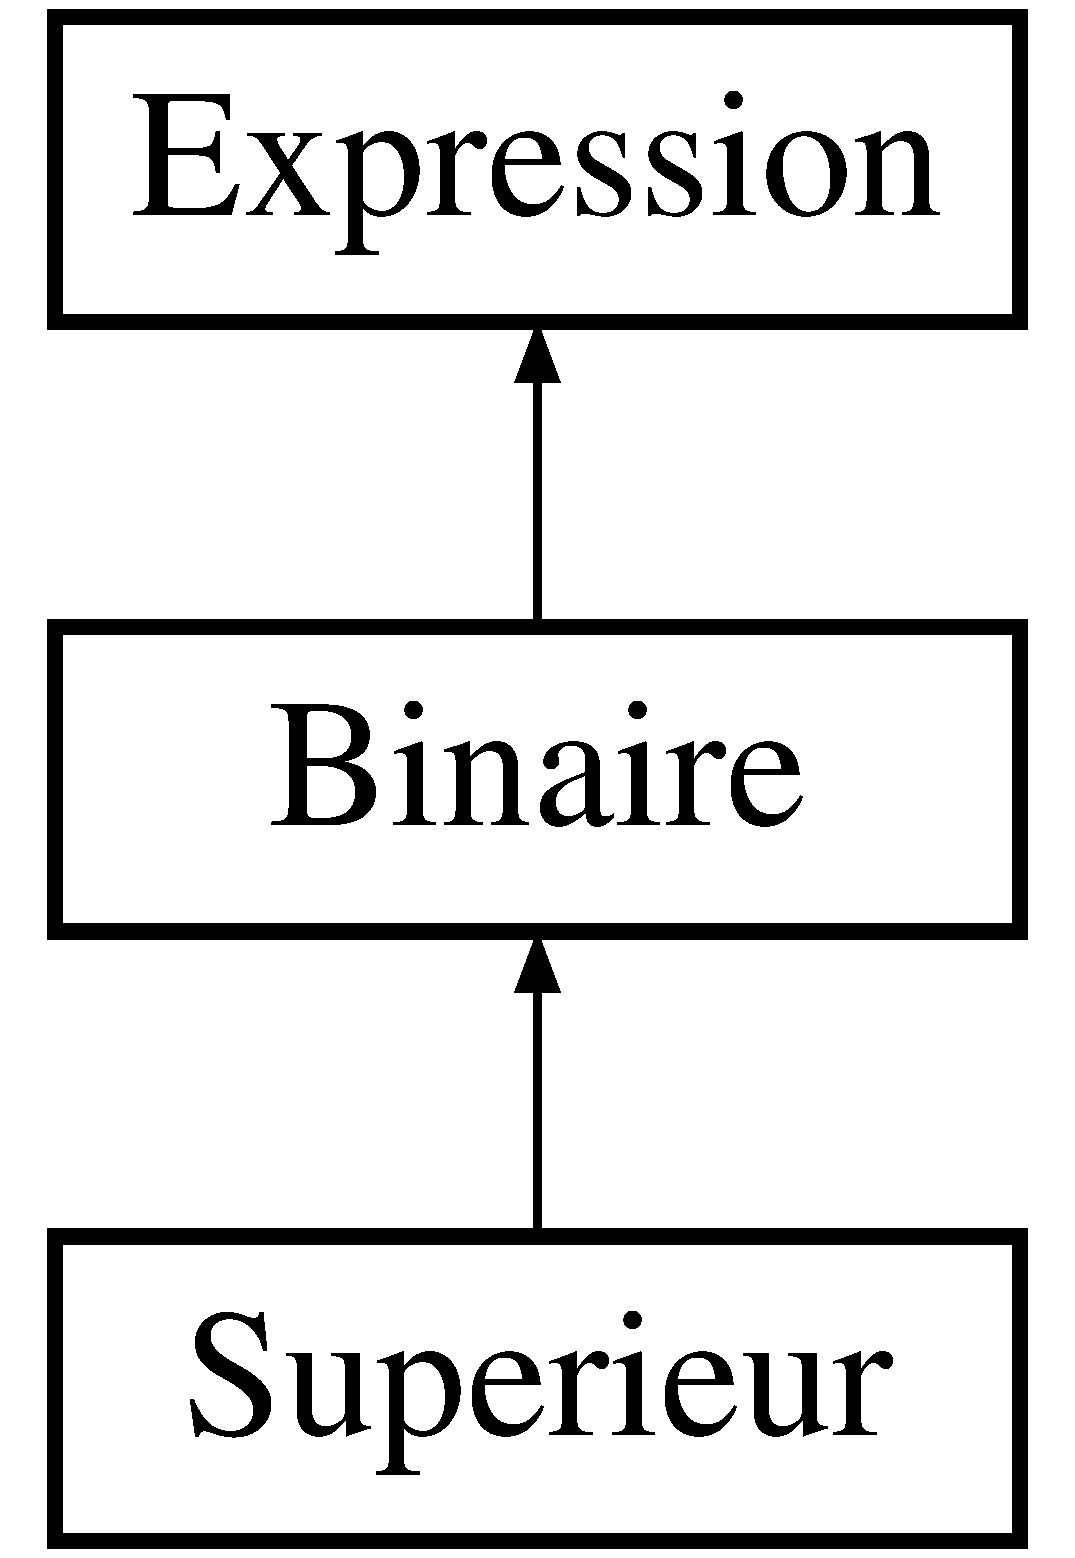
\includegraphics[height=3.000000cm]{class_superieur}
\end{center}
\end{figure}
\subsection*{Public Member Functions}
\begin{DoxyCompactItemize}
\item 
\hyperlink{class_superieur_a41d7c8a2c8ccbffdd05dc6331b453f0c}{Superieur} ()
\begin{DoxyCompactList}\small\item\em Constructeur. \end{DoxyCompactList}\item 
virtual \hyperlink{class_superieur_a7e225cb4884a1eb0a790c533983651c7}{$\sim$\+Superieur} ()
\begin{DoxyCompactList}\small\item\em Destructeur Destructeur de la classe \hyperlink{class_superieur}{Superieur}. \end{DoxyCompactList}\item 
double \hyperlink{class_superieur_aee2a8239ebc62ae3db015d2744013fb7}{eval} () const 
\begin{DoxyCompactList}\small\item\em Evalue l\textquotesingle{}expression Methode qui permet d\textquotesingle{}evaluer l\textquotesingle{}expression. \end{DoxyCompactList}\item 
\hyperlink{class_expression}{Expression} $\ast$ \hyperlink{class_superieur_a316ead2ea4d6451a6056947bd4f3cdbd}{deriver} (const string \&)
\begin{DoxyCompactList}\small\item\em Derive l\textquotesingle{}expression$\ast$ Methode qui permet deriver l\textquotesingle{}expression. \end{DoxyCompactList}\item 
\hyperlink{class_expression}{Expression} $\ast$ \hyperlink{class_superieur_abdf12b4d6d2a36a36ee48556c674aa00}{simplifier} ()
\begin{DoxyCompactList}\small\item\em Simplifie l\textquotesingle{}expression Methode qui permet de simplifier l\textquotesingle{}expression. \end{DoxyCompactList}\item 
\hyperlink{class_expression}{Expression} $\ast$ \hyperlink{class_superieur_a13e12cfa91154853de73d67518fb7795}{clone} () const 
\begin{DoxyCompactList}\small\item\em clone l\textquotesingle{}expression Methode qui permet de cloner l\textquotesingle{}expression \end{DoxyCompactList}\item 
string \hyperlink{class_superieur_a0613c6dc4df0de7cf6a4be2e45bcf0ac}{afficher} () const 
\begin{DoxyCompactList}\small\item\em Affiche l\textquotesingle{}expression Methode qui permet d\textquotesingle{}afficher l\textquotesingle{}expression. \end{DoxyCompactList}\item 
\hyperlink{class_superieur_ab5f7f19225a1f311c0c8e746b886685c}{Superieur} (\hyperlink{class_expression}{Expression} $\ast$, \hyperlink{class_expression}{Expression} $\ast$)
\begin{DoxyCompactList}\small\item\em Constructeur. \end{DoxyCompactList}\end{DoxyCompactItemize}
\subsection*{Friends}
\begin{DoxyCompactItemize}
\item 
ostream \& \hyperlink{class_superieur_a3cbc340e88060643b98338c8aebaa5ef}{operator$<$$<$} (ostream \&, const \hyperlink{class_superieur}{Superieur} \&)
\begin{DoxyCompactList}\small\item\em operator$<$$<$ Methode qui permet d\textquotesingle{}afficher l\textquotesingle{}expression \end{DoxyCompactList}\end{DoxyCompactItemize}
\subsection*{Additional Inherited Members}


\subsection{Detailed Description}
La classe \hyperlink{class_superieur}{Superieur}. 

Cette classe repr�sente les op�rateurs de comparaison strictement sup�rieur 

\subsection{Constructor \& Destructor Documentation}
\index{Superieur@{Superieur}!Superieur@{Superieur}}
\index{Superieur@{Superieur}!Superieur@{Superieur}}
\subsubsection[{\texorpdfstring{Superieur()}{Superieur()}}]{\setlength{\rightskip}{0pt plus 5cm}Superieur\+::\+Superieur (
\begin{DoxyParamCaption}
{}
\end{DoxyParamCaption}
)}\hypertarget{class_superieur_a41d7c8a2c8ccbffdd05dc6331b453f0c}{}\label{class_superieur_a41d7c8a2c8ccbffdd05dc6331b453f0c}


Constructeur. 

Constructeur de la classe \hyperlink{class_superieur}{Superieur} \index{Superieur@{Superieur}!````~Superieur@{$\sim$\+Superieur}}
\index{````~Superieur@{$\sim$\+Superieur}!Superieur@{Superieur}}
\subsubsection[{\texorpdfstring{$\sim$\+Superieur()}{~Superieur()}}]{\setlength{\rightskip}{0pt plus 5cm}Superieur\+::$\sim$\+Superieur (
\begin{DoxyParamCaption}
{}
\end{DoxyParamCaption}
)\hspace{0.3cm}{\ttfamily [virtual]}}\hypertarget{class_superieur_a7e225cb4884a1eb0a790c533983651c7}{}\label{class_superieur_a7e225cb4884a1eb0a790c533983651c7}


Destructeur Destructeur de la classe \hyperlink{class_superieur}{Superieur}. 

\index{Superieur@{Superieur}!Superieur@{Superieur}}
\index{Superieur@{Superieur}!Superieur@{Superieur}}
\subsubsection[{\texorpdfstring{Superieur(\+Expression $\ast$, Expression $\ast$)}{Superieur(Expression *, Expression *)}}]{\setlength{\rightskip}{0pt plus 5cm}Superieur\+::\+Superieur (
\begin{DoxyParamCaption}
\item[{{\bf Expression} $\ast$}]{exp1, }
\item[{{\bf Expression} $\ast$}]{exp2}
\end{DoxyParamCaption}
)}\hypertarget{class_superieur_ab5f7f19225a1f311c0c8e746b886685c}{}\label{class_superieur_ab5f7f19225a1f311c0c8e746b886685c}


Constructeur. 

Constructeur de la classe \hyperlink{class_superieur}{Superieur}


\begin{DoxyParams}{Parameters}
{\em exp1} & \+: op�rande gauche \\
\hline
{\em exp2} & \+: op�rande droite \\
\hline
\end{DoxyParams}


\subsection{Member Function Documentation}
\index{Superieur@{Superieur}!afficher@{afficher}}
\index{afficher@{afficher}!Superieur@{Superieur}}
\subsubsection[{\texorpdfstring{afficher() const }{afficher() const }}]{\setlength{\rightskip}{0pt plus 5cm}string Superieur\+::afficher (
\begin{DoxyParamCaption}
{}
\end{DoxyParamCaption}
) const\hspace{0.3cm}{\ttfamily [virtual]}}\hypertarget{class_superieur_a0613c6dc4df0de7cf6a4be2e45bcf0ac}{}\label{class_superieur_a0613c6dc4df0de7cf6a4be2e45bcf0ac}


Affiche l\textquotesingle{}expression Methode qui permet d\textquotesingle{}afficher l\textquotesingle{}expression. 

\begin{DoxyReturn}{Returns}
Le string d\textquotesingle{}expression 
\end{DoxyReturn}


Reimplemented from \hyperlink{class_expression_a953c7de0302331023987a2fff895cb85}{Expression}.

\index{Superieur@{Superieur}!clone@{clone}}
\index{clone@{clone}!Superieur@{Superieur}}
\subsubsection[{\texorpdfstring{clone() const }{clone() const }}]{\setlength{\rightskip}{0pt plus 5cm}{\bf Expression} $\ast$ Superieur\+::clone (
\begin{DoxyParamCaption}
{}
\end{DoxyParamCaption}
) const\hspace{0.3cm}{\ttfamily [virtual]}}\hypertarget{class_superieur_a13e12cfa91154853de73d67518fb7795}{}\label{class_superieur_a13e12cfa91154853de73d67518fb7795}


clone l\textquotesingle{}expression Methode qui permet de cloner l\textquotesingle{}expression 

\begin{DoxyReturn}{Returns}
L\textquotesingle{}expression clon� 
\end{DoxyReturn}


Implements \hyperlink{class_expression_ac9fcea09ddd3a650a92c3606118abfb6}{Expression}.

\index{Superieur@{Superieur}!deriver@{deriver}}
\index{deriver@{deriver}!Superieur@{Superieur}}
\subsubsection[{\texorpdfstring{deriver(const string \&)}{deriver(const string &)}}]{\setlength{\rightskip}{0pt plus 5cm}{\bf Expression} $\ast$ Superieur\+::deriver (
\begin{DoxyParamCaption}
\item[{const string \&}]{var}
\end{DoxyParamCaption}
)\hspace{0.3cm}{\ttfamily [virtual]}}\hypertarget{class_superieur_a316ead2ea4d6451a6056947bd4f3cdbd}{}\label{class_superieur_a316ead2ea4d6451a6056947bd4f3cdbd}


Derive l\textquotesingle{}expression$\ast$ Methode qui permet deriver l\textquotesingle{}expression. 

\begin{DoxyReturn}{Returns}
L\textquotesingle{}expression deriv� 
\end{DoxyReturn}


Implements \hyperlink{class_expression_a0a2a2cf2cdb1e8ca556ad59832784193}{Expression}.

\index{Superieur@{Superieur}!eval@{eval}}
\index{eval@{eval}!Superieur@{Superieur}}
\subsubsection[{\texorpdfstring{eval() const }{eval() const }}]{\setlength{\rightskip}{0pt plus 5cm}double Superieur\+::eval (
\begin{DoxyParamCaption}
{}
\end{DoxyParamCaption}
) const\hspace{0.3cm}{\ttfamily [virtual]}}\hypertarget{class_superieur_aee2a8239ebc62ae3db015d2744013fb7}{}\label{class_superieur_aee2a8239ebc62ae3db015d2744013fb7}


Evalue l\textquotesingle{}expression Methode qui permet d\textquotesingle{}evaluer l\textquotesingle{}expression. 

\begin{DoxyReturn}{Returns}
Le valeur d\textquotesingle{}expression 
\end{DoxyReturn}


Implements \hyperlink{class_expression_a5481c36265e11eff513df87bbc5a1d33}{Expression}.

\index{Superieur@{Superieur}!simplifier@{simplifier}}
\index{simplifier@{simplifier}!Superieur@{Superieur}}
\subsubsection[{\texorpdfstring{simplifier()}{simplifier()}}]{\setlength{\rightskip}{0pt plus 5cm}{\bf Expression} $\ast$ Superieur\+::simplifier (
\begin{DoxyParamCaption}
{}
\end{DoxyParamCaption}
)\hspace{0.3cm}{\ttfamily [virtual]}}\hypertarget{class_superieur_abdf12b4d6d2a36a36ee48556c674aa00}{}\label{class_superieur_abdf12b4d6d2a36a36ee48556c674aa00}


Simplifie l\textquotesingle{}expression Methode qui permet de simplifier l\textquotesingle{}expression. 

\begin{DoxyReturn}{Returns}
L\textquotesingle{}expression simplifi� 
\end{DoxyReturn}


Implements \hyperlink{class_expression_a319d06d43ead325c835181419061ae0b}{Expression}.



\subsection{Friends And Related Function Documentation}
\index{Superieur@{Superieur}!operator$<$$<$@{operator$<$$<$}}
\index{operator$<$$<$@{operator$<$$<$}!Superieur@{Superieur}}
\subsubsection[{\texorpdfstring{operator$<$$<$}{operator<<}}]{\setlength{\rightskip}{0pt plus 5cm}ostream\& operator$<$$<$ (
\begin{DoxyParamCaption}
\item[{ostream \&}]{os, }
\item[{const {\bf Superieur} \&}]{a}
\end{DoxyParamCaption}
)\hspace{0.3cm}{\ttfamily [friend]}}\hypertarget{class_superieur_a3cbc340e88060643b98338c8aebaa5ef}{}\label{class_superieur_a3cbc340e88060643b98338c8aebaa5ef}


operator$<$$<$ Methode qui permet d\textquotesingle{}afficher l\textquotesingle{}expression 



The documentation for this class was generated from the following files\+:\begin{DoxyCompactItemize}
\item 
include/\hyperlink{binaire_8h}{binaire.\+h}\item 
src/\hyperlink{binaire_8cpp}{binaire.\+cpp}\end{DoxyCompactItemize}

\hypertarget{class_superieur_egal}{}\section{Superieur\+Egal Class Reference}
\label{class_superieur_egal}\index{Superieur\+Egal@{Superieur\+Egal}}


La classe \hyperlink{class_superieur_egal}{Superieur\+Egal}.  




{\ttfamily \#include $<$binaire.\+h$>$}

Inheritance diagram for Superieur\+Egal\+:\begin{figure}[H]
\begin{center}
\leavevmode
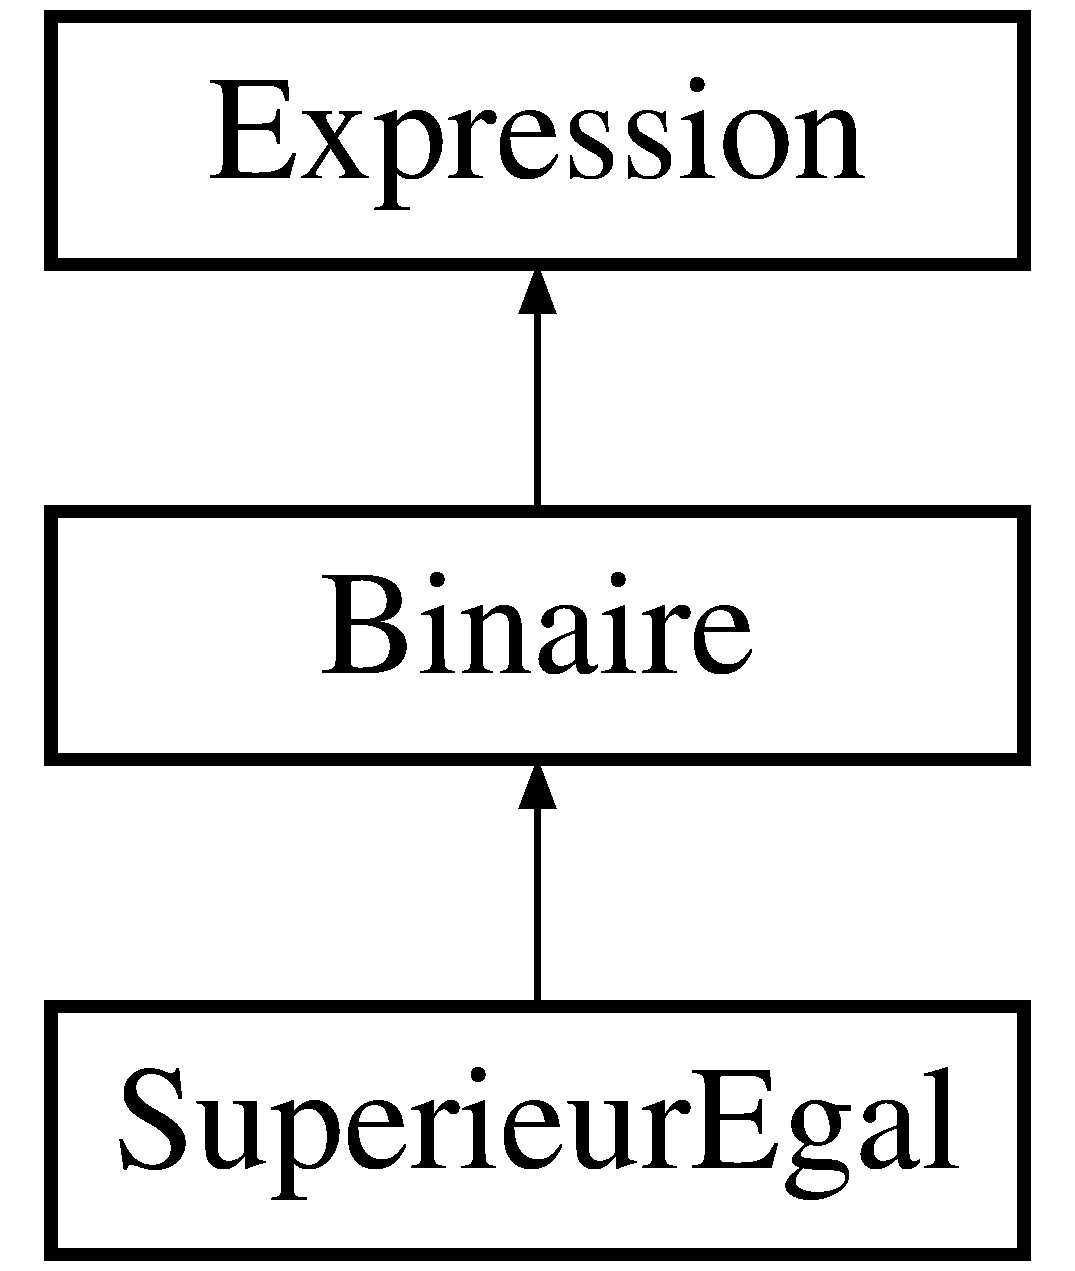
\includegraphics[height=3.000000cm]{class_superieur_egal}
\end{center}
\end{figure}
\subsection*{Public Member Functions}
\begin{DoxyCompactItemize}
\item 
\hyperlink{class_superieur_egal_aaa93c9c3b421c4c6bb058d64304e75f1}{Superieur\+Egal} ()
\begin{DoxyCompactList}\small\item\em Constructeur. \end{DoxyCompactList}\item 
virtual \hyperlink{class_superieur_egal_a1d889421762a84aac2c0109011f2b615}{$\sim$\+Superieur\+Egal} ()
\begin{DoxyCompactList}\small\item\em Destructeur Destructeur de la classe \hyperlink{class_superieur_egal}{Superieur\+Egal}. \end{DoxyCompactList}\item 
double \hyperlink{class_superieur_egal_a1ea7bc313de485e4055914661d5e596a}{eval} () const 
\begin{DoxyCompactList}\small\item\em Evalue l\textquotesingle{}expression Methode qui permet d\textquotesingle{}evaluer l\textquotesingle{}expression. \end{DoxyCompactList}\item 
\hyperlink{class_expression}{Expression} $\ast$ \hyperlink{class_superieur_egal_ae1aa499c6130c12a96910df1f6776fac}{deriver} (const string \&)
\begin{DoxyCompactList}\small\item\em Derive l\textquotesingle{}expression$\ast$ Methode qui permet deriver l\textquotesingle{}expression. \end{DoxyCompactList}\item 
\hyperlink{class_expression}{Expression} $\ast$ \hyperlink{class_superieur_egal_a8df045c9b0a436106ccc3e51b7d7d21d}{simplifier} ()
\begin{DoxyCompactList}\small\item\em Simplifie l\textquotesingle{}expression Methode qui permet de simplifier l\textquotesingle{}expression. \end{DoxyCompactList}\item 
\hyperlink{class_expression}{Expression} $\ast$ \hyperlink{class_superieur_egal_a55d16bacf7aff0cf9c8a7b4992b09279}{clone} () const 
\begin{DoxyCompactList}\small\item\em clone l\textquotesingle{}expression Methode qui permet de cloner l\textquotesingle{}expression \end{DoxyCompactList}\item 
string \hyperlink{class_superieur_egal_a9fb8d0b7cdfb75361bae0a2fa8db06a0}{afficher} () const 
\begin{DoxyCompactList}\small\item\em Affiche l\textquotesingle{}expression Methode qui permet d\textquotesingle{}afficher l\textquotesingle{}expression. \end{DoxyCompactList}\item 
\hyperlink{class_superieur_egal_abaff44b6ec10407547de0dcfcceb18b0}{Superieur\+Egal} (\hyperlink{class_expression}{Expression} $\ast$, \hyperlink{class_expression}{Expression} $\ast$)
\begin{DoxyCompactList}\small\item\em Constructeur. \end{DoxyCompactList}\end{DoxyCompactItemize}
\subsection*{Friends}
\begin{DoxyCompactItemize}
\item 
ostream \& \hyperlink{class_superieur_egal_aae7d1916ebb0785c18a7a1123e99467e}{operator$<$$<$} (ostream \&, const \hyperlink{class_superieur_egal}{Superieur\+Egal} \&)
\begin{DoxyCompactList}\small\item\em operator$<$$<$ Methode qui permet d\textquotesingle{}afficher l\textquotesingle{}expression \end{DoxyCompactList}\end{DoxyCompactItemize}
\subsection*{Additional Inherited Members}


\subsection{Detailed Description}
La classe \hyperlink{class_superieur_egal}{Superieur\+Egal}. 

Cette classe repr�sente les op�rateurs de comparaison sup�rieur ou �gal 

\subsection{Constructor \& Destructor Documentation}
\index{Superieur\+Egal@{Superieur\+Egal}!Superieur\+Egal@{Superieur\+Egal}}
\index{Superieur\+Egal@{Superieur\+Egal}!Superieur\+Egal@{Superieur\+Egal}}
\subsubsection[{\texorpdfstring{Superieur\+Egal()}{SuperieurEgal()}}]{\setlength{\rightskip}{0pt plus 5cm}Superieur\+Egal\+::\+Superieur\+Egal (
\begin{DoxyParamCaption}
{}
\end{DoxyParamCaption}
)}\hypertarget{class_superieur_egal_aaa93c9c3b421c4c6bb058d64304e75f1}{}\label{class_superieur_egal_aaa93c9c3b421c4c6bb058d64304e75f1}


Constructeur. 

Constructeur de la classe \hyperlink{class_superieur_egal}{Superieur\+Egal} \index{Superieur\+Egal@{Superieur\+Egal}!````~Superieur\+Egal@{$\sim$\+Superieur\+Egal}}
\index{````~Superieur\+Egal@{$\sim$\+Superieur\+Egal}!Superieur\+Egal@{Superieur\+Egal}}
\subsubsection[{\texorpdfstring{$\sim$\+Superieur\+Egal()}{~SuperieurEgal()}}]{\setlength{\rightskip}{0pt plus 5cm}Superieur\+Egal\+::$\sim$\+Superieur\+Egal (
\begin{DoxyParamCaption}
{}
\end{DoxyParamCaption}
)\hspace{0.3cm}{\ttfamily [virtual]}}\hypertarget{class_superieur_egal_a1d889421762a84aac2c0109011f2b615}{}\label{class_superieur_egal_a1d889421762a84aac2c0109011f2b615}


Destructeur Destructeur de la classe \hyperlink{class_superieur_egal}{Superieur\+Egal}. 

\index{Superieur\+Egal@{Superieur\+Egal}!Superieur\+Egal@{Superieur\+Egal}}
\index{Superieur\+Egal@{Superieur\+Egal}!Superieur\+Egal@{Superieur\+Egal}}
\subsubsection[{\texorpdfstring{Superieur\+Egal(\+Expression $\ast$, Expression $\ast$)}{SuperieurEgal(Expression *, Expression *)}}]{\setlength{\rightskip}{0pt plus 5cm}Superieur\+Egal\+::\+Superieur\+Egal (
\begin{DoxyParamCaption}
\item[{{\bf Expression} $\ast$}]{exp1, }
\item[{{\bf Expression} $\ast$}]{exp2}
\end{DoxyParamCaption}
)}\hypertarget{class_superieur_egal_abaff44b6ec10407547de0dcfcceb18b0}{}\label{class_superieur_egal_abaff44b6ec10407547de0dcfcceb18b0}


Constructeur. 

Constructeur de la classe \hyperlink{class_superieur_egal}{Superieur\+Egal}


\begin{DoxyParams}{Parameters}
{\em exp1} & \+: op�rande gauche \\
\hline
{\em exp2} & \+: op�rande droite \\
\hline
\end{DoxyParams}


\subsection{Member Function Documentation}
\index{Superieur\+Egal@{Superieur\+Egal}!afficher@{afficher}}
\index{afficher@{afficher}!Superieur\+Egal@{Superieur\+Egal}}
\subsubsection[{\texorpdfstring{afficher() const }{afficher() const }}]{\setlength{\rightskip}{0pt plus 5cm}string Superieur\+Egal\+::afficher (
\begin{DoxyParamCaption}
{}
\end{DoxyParamCaption}
) const\hspace{0.3cm}{\ttfamily [virtual]}}\hypertarget{class_superieur_egal_a9fb8d0b7cdfb75361bae0a2fa8db06a0}{}\label{class_superieur_egal_a9fb8d0b7cdfb75361bae0a2fa8db06a0}


Affiche l\textquotesingle{}expression Methode qui permet d\textquotesingle{}afficher l\textquotesingle{}expression. 

\begin{DoxyReturn}{Returns}
Le string d\textquotesingle{}expression 
\end{DoxyReturn}


Reimplemented from \hyperlink{class_expression_a953c7de0302331023987a2fff895cb85}{Expression}.

\index{Superieur\+Egal@{Superieur\+Egal}!clone@{clone}}
\index{clone@{clone}!Superieur\+Egal@{Superieur\+Egal}}
\subsubsection[{\texorpdfstring{clone() const }{clone() const }}]{\setlength{\rightskip}{0pt plus 5cm}{\bf Expression} $\ast$ Superieur\+Egal\+::clone (
\begin{DoxyParamCaption}
{}
\end{DoxyParamCaption}
) const\hspace{0.3cm}{\ttfamily [virtual]}}\hypertarget{class_superieur_egal_a55d16bacf7aff0cf9c8a7b4992b09279}{}\label{class_superieur_egal_a55d16bacf7aff0cf9c8a7b4992b09279}


clone l\textquotesingle{}expression Methode qui permet de cloner l\textquotesingle{}expression 

\begin{DoxyReturn}{Returns}
L\textquotesingle{}expression clon� 
\end{DoxyReturn}


Implements \hyperlink{class_expression_ac9fcea09ddd3a650a92c3606118abfb6}{Expression}.

\index{Superieur\+Egal@{Superieur\+Egal}!deriver@{deriver}}
\index{deriver@{deriver}!Superieur\+Egal@{Superieur\+Egal}}
\subsubsection[{\texorpdfstring{deriver(const string \&)}{deriver(const string &)}}]{\setlength{\rightskip}{0pt plus 5cm}{\bf Expression} $\ast$ Superieur\+Egal\+::deriver (
\begin{DoxyParamCaption}
\item[{const string \&}]{var}
\end{DoxyParamCaption}
)\hspace{0.3cm}{\ttfamily [virtual]}}\hypertarget{class_superieur_egal_ae1aa499c6130c12a96910df1f6776fac}{}\label{class_superieur_egal_ae1aa499c6130c12a96910df1f6776fac}


Derive l\textquotesingle{}expression$\ast$ Methode qui permet deriver l\textquotesingle{}expression. 

\begin{DoxyReturn}{Returns}
L\textquotesingle{}expression deriv� 
\end{DoxyReturn}


Implements \hyperlink{class_expression_a0a2a2cf2cdb1e8ca556ad59832784193}{Expression}.

\index{Superieur\+Egal@{Superieur\+Egal}!eval@{eval}}
\index{eval@{eval}!Superieur\+Egal@{Superieur\+Egal}}
\subsubsection[{\texorpdfstring{eval() const }{eval() const }}]{\setlength{\rightskip}{0pt plus 5cm}double Superieur\+Egal\+::eval (
\begin{DoxyParamCaption}
{}
\end{DoxyParamCaption}
) const\hspace{0.3cm}{\ttfamily [virtual]}}\hypertarget{class_superieur_egal_a1ea7bc313de485e4055914661d5e596a}{}\label{class_superieur_egal_a1ea7bc313de485e4055914661d5e596a}


Evalue l\textquotesingle{}expression Methode qui permet d\textquotesingle{}evaluer l\textquotesingle{}expression. 

\begin{DoxyReturn}{Returns}
Le valeur d\textquotesingle{}expression 
\end{DoxyReturn}


Implements \hyperlink{class_expression_a5481c36265e11eff513df87bbc5a1d33}{Expression}.

\index{Superieur\+Egal@{Superieur\+Egal}!simplifier@{simplifier}}
\index{simplifier@{simplifier}!Superieur\+Egal@{Superieur\+Egal}}
\subsubsection[{\texorpdfstring{simplifier()}{simplifier()}}]{\setlength{\rightskip}{0pt plus 5cm}{\bf Expression} $\ast$ Superieur\+Egal\+::simplifier (
\begin{DoxyParamCaption}
{}
\end{DoxyParamCaption}
)\hspace{0.3cm}{\ttfamily [virtual]}}\hypertarget{class_superieur_egal_a8df045c9b0a436106ccc3e51b7d7d21d}{}\label{class_superieur_egal_a8df045c9b0a436106ccc3e51b7d7d21d}


Simplifie l\textquotesingle{}expression Methode qui permet de simplifier l\textquotesingle{}expression. 

\begin{DoxyReturn}{Returns}
L\textquotesingle{}expression simplifi� 
\end{DoxyReturn}


Implements \hyperlink{class_expression_a319d06d43ead325c835181419061ae0b}{Expression}.



\subsection{Friends And Related Function Documentation}
\index{Superieur\+Egal@{Superieur\+Egal}!operator$<$$<$@{operator$<$$<$}}
\index{operator$<$$<$@{operator$<$$<$}!Superieur\+Egal@{Superieur\+Egal}}
\subsubsection[{\texorpdfstring{operator$<$$<$}{operator<<}}]{\setlength{\rightskip}{0pt plus 5cm}ostream\& operator$<$$<$ (
\begin{DoxyParamCaption}
\item[{ostream \&}]{os, }
\item[{const {\bf Superieur\+Egal} \&}]{a}
\end{DoxyParamCaption}
)\hspace{0.3cm}{\ttfamily [friend]}}\hypertarget{class_superieur_egal_aae7d1916ebb0785c18a7a1123e99467e}{}\label{class_superieur_egal_aae7d1916ebb0785c18a7a1123e99467e}


operator$<$$<$ Methode qui permet d\textquotesingle{}afficher l\textquotesingle{}expression 



The documentation for this class was generated from the following files\+:\begin{DoxyCompactItemize}
\item 
include/\hyperlink{binaire_8h}{binaire.\+h}\item 
src/\hyperlink{binaire_8cpp}{binaire.\+cpp}\end{DoxyCompactItemize}

\hypertarget{class_unaire}{}\section{Unaire Class Reference}
\label{class_unaire}\index{Unaire@{Unaire}}


La classe \hyperlink{class_unaire}{Unaire}.  




{\ttfamily \#include $<$unaire.\+h$>$}

Inheritance diagram for Unaire\+:\begin{figure}[H]
\begin{center}
\leavevmode
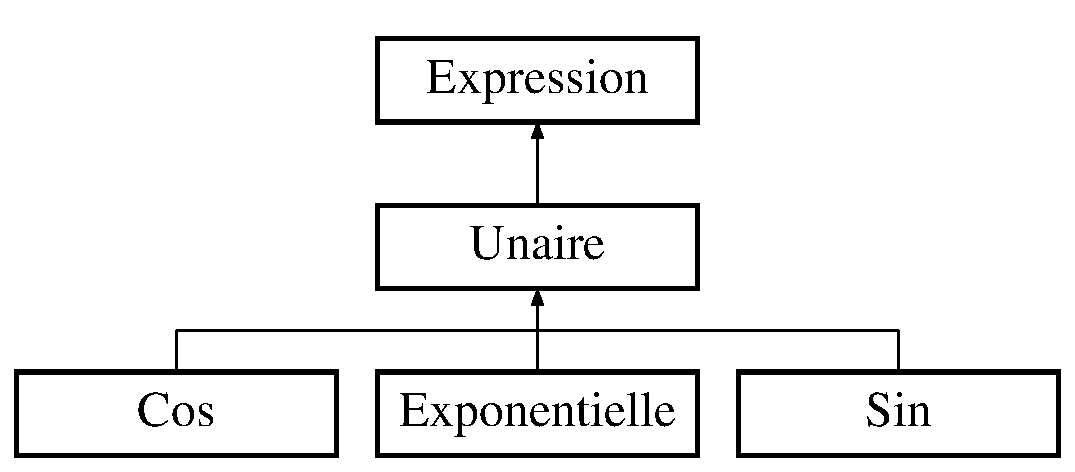
\includegraphics[height=3.000000cm]{class_unaire}
\end{center}
\end{figure}
\subsection*{Public Member Functions}
\begin{DoxyCompactItemize}
\item 
\hyperlink{class_unaire_ab10daf7797b8a7c1d81742883269eb47}{Unaire} ()
\begin{DoxyCompactList}\small\item\em Constructeur. \end{DoxyCompactList}\item 
\hyperlink{class_unaire_a0825cb8fa23c18b8e35d156ecb7ec692}{Unaire} (\hyperlink{class_expression}{Expression} $\ast$, const string \&name=\char`\"{}unaire\char`\"{})
\begin{DoxyCompactList}\small\item\em Constructeur. \end{DoxyCompactList}\item 
virtual \hyperlink{class_unaire_a7a733b0533aa3a688fb3ced70c73f013}{$\sim$\+Unaire} ()
\begin{DoxyCompactList}\small\item\em Destructeur Destructeur de la classe \hyperlink{class_affectation}{Affectation}. \end{DoxyCompactList}\item 
virtual string \hyperlink{class_unaire_a992fb04dc38a52b194e0f85e332ca30e}{afficher} ()
\begin{DoxyCompactList}\small\item\em Affiche l\textquotesingle{}expression Methode qui permet d\textquotesingle{}afficher l\textquotesingle{}expression. \end{DoxyCompactList}\end{DoxyCompactItemize}
\subsection*{Protected Attributes}
\begin{DoxyCompactItemize}
\item 
\hyperlink{class_expression}{Expression} $\ast$ \hyperlink{class_unaire_adfb8ac6625a88f0b671ebc86383d77bf}{\+\_\+op}
\end{DoxyCompactItemize}
\subsection*{Additional Inherited Members}


\subsection{Detailed Description}
La classe \hyperlink{class_unaire}{Unaire}. 

Cette classe repr�sente les op�rateurs unaires. Ces operateur agissent sur un seul op�rande qui peut-\/�tre une constante, une variable, ou une expression. 

\subsection{Constructor \& Destructor Documentation}
\index{Unaire@{Unaire}!Unaire@{Unaire}}
\index{Unaire@{Unaire}!Unaire@{Unaire}}
\subsubsection[{\texorpdfstring{Unaire()}{Unaire()}}]{\setlength{\rightskip}{0pt plus 5cm}Unaire\+::\+Unaire (
\begin{DoxyParamCaption}
{}
\end{DoxyParamCaption}
)}\hypertarget{class_unaire_ab10daf7797b8a7c1d81742883269eb47}{}\label{class_unaire_ab10daf7797b8a7c1d81742883269eb47}


Constructeur. 

Constructeur de la classe \hyperlink{class_unaire}{Unaire} \index{Unaire@{Unaire}!Unaire@{Unaire}}
\index{Unaire@{Unaire}!Unaire@{Unaire}}
\subsubsection[{\texorpdfstring{Unaire(\+Expression $\ast$, const string \&name=""unaire"")}{Unaire(Expression *, const string &name="unaire")}}]{\setlength{\rightskip}{0pt plus 5cm}Unaire\+::\+Unaire (
\begin{DoxyParamCaption}
\item[{{\bf Expression} $\ast$}]{op, }
\item[{const string \&}]{name = {\ttfamily \char`\"{}unaire\char`\"{}}}
\end{DoxyParamCaption}
)}\hypertarget{class_unaire_a0825cb8fa23c18b8e35d156ecb7ec692}{}\label{class_unaire_a0825cb8fa23c18b8e35d156ecb7ec692}


Constructeur. 

Constructeur de la classe \hyperlink{class_unaire}{Unaire}


\begin{DoxyParams}{Parameters}
{\em exp} & \+: l\textquotesingle{}expression \\
\hline
{\em nom} & \+: le nom \\
\hline
\end{DoxyParams}
\index{Unaire@{Unaire}!````~Unaire@{$\sim$\+Unaire}}
\index{````~Unaire@{$\sim$\+Unaire}!Unaire@{Unaire}}
\subsubsection[{\texorpdfstring{$\sim$\+Unaire()}{~Unaire()}}]{\setlength{\rightskip}{0pt plus 5cm}Unaire\+::$\sim$\+Unaire (
\begin{DoxyParamCaption}
{}
\end{DoxyParamCaption}
)\hspace{0.3cm}{\ttfamily [virtual]}}\hypertarget{class_unaire_a7a733b0533aa3a688fb3ced70c73f013}{}\label{class_unaire_a7a733b0533aa3a688fb3ced70c73f013}


Destructeur Destructeur de la classe \hyperlink{class_affectation}{Affectation}. 



\subsection{Member Function Documentation}
\index{Unaire@{Unaire}!afficher@{afficher}}
\index{afficher@{afficher}!Unaire@{Unaire}}
\subsubsection[{\texorpdfstring{afficher()}{afficher()}}]{\setlength{\rightskip}{0pt plus 5cm}string Unaire\+::afficher (
\begin{DoxyParamCaption}
{}
\end{DoxyParamCaption}
)\hspace{0.3cm}{\ttfamily [virtual]}}\hypertarget{class_unaire_a992fb04dc38a52b194e0f85e332ca30e}{}\label{class_unaire_a992fb04dc38a52b194e0f85e332ca30e}


Affiche l\textquotesingle{}expression Methode qui permet d\textquotesingle{}afficher l\textquotesingle{}expression. 

\begin{DoxyReturn}{Returns}
Le string d\textquotesingle{}expression 
\end{DoxyReturn}


\subsection{Member Data Documentation}
\index{Unaire@{Unaire}!\+\_\+op@{\+\_\+op}}
\index{\+\_\+op@{\+\_\+op}!Unaire@{Unaire}}
\subsubsection[{\texorpdfstring{\+\_\+op}{_op}}]{\setlength{\rightskip}{0pt plus 5cm}{\bf Expression}$\ast$ Unaire\+::\+\_\+op\hspace{0.3cm}{\ttfamily [protected]}}\hypertarget{class_unaire_adfb8ac6625a88f0b671ebc86383d77bf}{}\label{class_unaire_adfb8ac6625a88f0b671ebc86383d77bf}


The documentation for this class was generated from the following files\+:\begin{DoxyCompactItemize}
\item 
include/\hyperlink{unaire_8h}{unaire.\+h}\item 
src/\hyperlink{unaire_8cpp}{unaire.\+cpp}\end{DoxyCompactItemize}

\hypertarget{class_variable}{}\section{Variable Class Reference}
\label{class_variable}\index{Variable@{Variable}}


La classe \hyperlink{class_variable}{Variable}.  




{\ttfamily \#include $<$variable.\+h$>$}

Inheritance diagram for Variable\+:\begin{figure}[H]
\begin{center}
\leavevmode
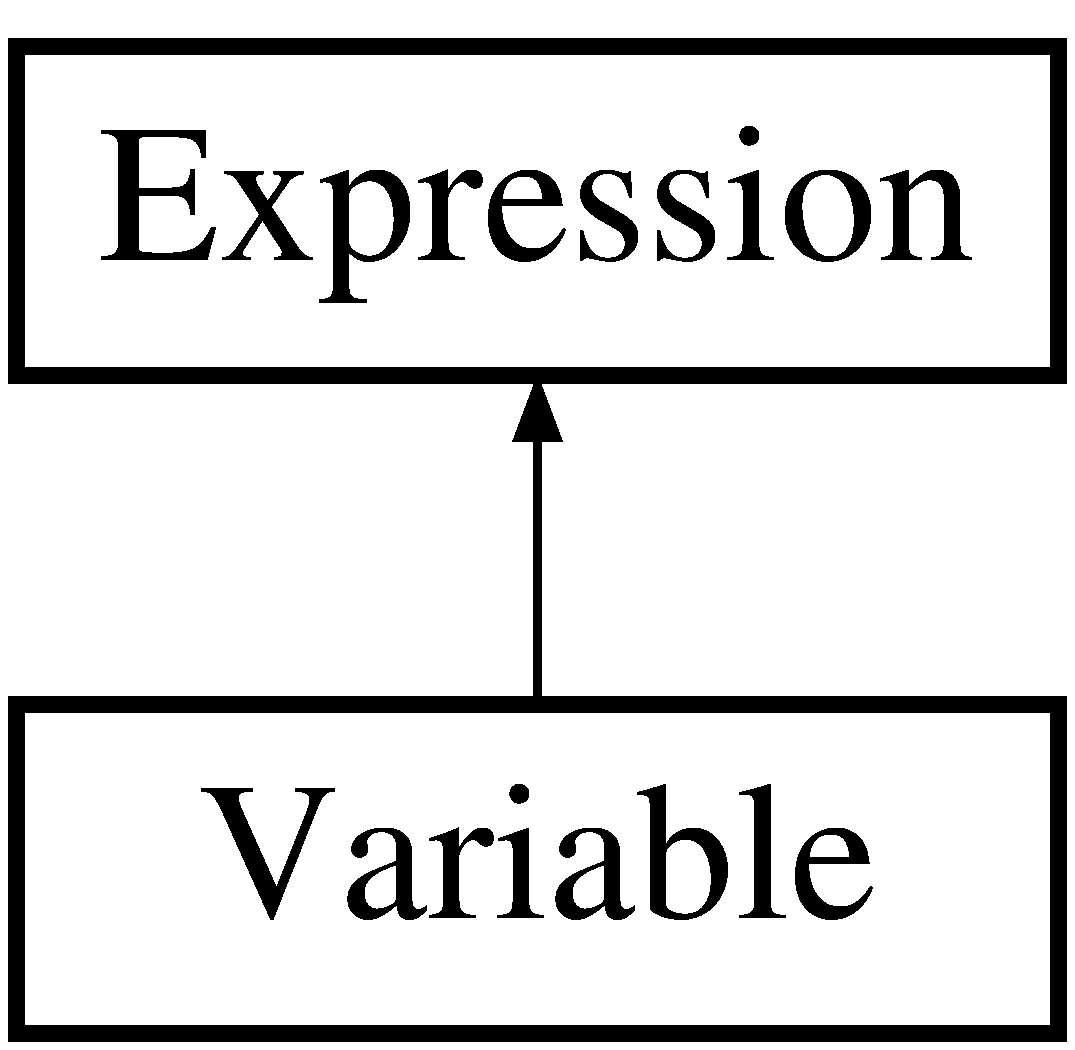
\includegraphics[height=2.000000cm]{class_variable}
\end{center}
\end{figure}
\subsection*{Public Member Functions}
\begin{DoxyCompactItemize}
\item 
\hyperlink{class_variable_a601d7302bd602908e852db38ab066fb8}{Variable} (const string \&, double)
\begin{DoxyCompactList}\small\item\em Constructeur. \end{DoxyCompactList}\item 
\hyperlink{class_variable_a5716c9dcafcc8cf59a6f6b5dac3ec7a2}{Variable} ()
\begin{DoxyCompactList}\small\item\em Constructeur. \end{DoxyCompactList}\item 
\hyperlink{class_variable_a96ce3df790172b8ad9e7bbf540d38bf3}{Variable} (const string \&)
\begin{DoxyCompactList}\small\item\em Constructeur. \end{DoxyCompactList}\item 
double \hyperlink{class_variable_a4bb6309ec2c117c5c050ca89488daf2e}{eval} () const 
\begin{DoxyCompactList}\small\item\em Evalue l\textquotesingle{}expression Methode qui permet d\textquotesingle{}evaluer l\textquotesingle{}expression. \end{DoxyCompactList}\item 
\hyperlink{class_expression}{Expression} $\ast$ \hyperlink{class_variable_ae7e8e77718b47b10f7633756715aa986}{deriver} (const string \&)
\begin{DoxyCompactList}\small\item\em Derive l\textquotesingle{}expression$\ast$ Methode qui permet deriver l\textquotesingle{}expression. \end{DoxyCompactList}\item 
\hyperlink{class_expression}{Expression} $\ast$ \hyperlink{class_variable_a60c5ae49c674293b68646342c9de242f}{simplifier} ()
\begin{DoxyCompactList}\small\item\em Simplifie l\textquotesingle{}expression Methode qui permet de simplifier l\textquotesingle{}expression. \end{DoxyCompactList}\item 
virtual \hyperlink{class_variable_acfc14d0ad77af53025f890b4d3a7745a}{$\sim$\+Variable} ()
\begin{DoxyCompactList}\small\item\em Destructeur Destructeur de la classe \hyperlink{class_affectation}{Affectation}. \end{DoxyCompactList}\item 
string \hyperlink{class_variable_a2ae42f5b49f09c593be81f301462f1b3}{afficher} () const 
\begin{DoxyCompactList}\small\item\em Affiche l\textquotesingle{}expression Methode qui permet d\textquotesingle{}afficher l\textquotesingle{}expression. \end{DoxyCompactList}\item 
\hyperlink{class_expression}{Expression} $\ast$ \hyperlink{class_variable_a0862fa73db06e1c7f6fdd82dd7c3fc24}{clone} () const 
\begin{DoxyCompactList}\small\item\em clone l\textquotesingle{}expression Methode qui permet de cloner l\textquotesingle{}expression \end{DoxyCompactList}\item 
double \hyperlink{class_variable_a1edee492eaac2d45905122190d212060}{set} (double)
\begin{DoxyCompactList}\small\item\em Affecte la une valeur a une variable Methode qui permet d\textquotesingle{}affecter une valeur a un variable. \end{DoxyCompactList}\end{DoxyCompactItemize}
\subsection*{Static Public Member Functions}
\begin{DoxyCompactItemize}
\item 
static void \hyperlink{class_variable_a29b2557b27e881585651e459d22e5feb}{effacer\+Memoire} ()
\begin{DoxyCompactList}\small\item\em Efface la memoire Methode qui permet d\textquotesingle{}effacer le contenu de la m�moire (toutes les variables) \end{DoxyCompactList}\end{DoxyCompactItemize}
\subsection*{Friends}
\begin{DoxyCompactItemize}
\item 
ostream \& \hyperlink{class_variable_a627a5fdd79e8f7701199491a08c1593d}{operator$<$$<$} (ostream \&, const \hyperlink{class_variable}{Variable} \&)
\begin{DoxyCompactList}\small\item\em operator$<$$<$ Methode qui permet d\textquotesingle{}afficher l\textquotesingle{}expression \end{DoxyCompactList}\end{DoxyCompactItemize}
\subsection*{Additional Inherited Members}


\subsection{Detailed Description}
La classe \hyperlink{class_variable}{Variable}. 

Cette classe repr�sente les variables. 

\subsection{Constructor \& Destructor Documentation}
\index{Variable@{Variable}!Variable@{Variable}}
\index{Variable@{Variable}!Variable@{Variable}}
\subsubsection[{\texorpdfstring{Variable(const string \&, double)}{Variable(const string &, double)}}]{\setlength{\rightskip}{0pt plus 5cm}Variable\+::\+Variable (
\begin{DoxyParamCaption}
\item[{const string \&}]{id, }
\item[{double}]{valeur}
\end{DoxyParamCaption}
)}\hypertarget{class_variable_a601d7302bd602908e852db38ab066fb8}{}\label{class_variable_a601d7302bd602908e852db38ab066fb8}


Constructeur. 

Constructeur de la classe \hyperlink{class_variable}{Variable}


\begin{DoxyParams}{Parameters}
{\em id} & \+: le nom \\
\hline
{\em val} & \+: le valeur \\
\hline
\end{DoxyParams}
\index{Variable@{Variable}!Variable@{Variable}}
\index{Variable@{Variable}!Variable@{Variable}}
\subsubsection[{\texorpdfstring{Variable()}{Variable()}}]{\setlength{\rightskip}{0pt plus 5cm}Variable\+::\+Variable (
\begin{DoxyParamCaption}
{}
\end{DoxyParamCaption}
)}\hypertarget{class_variable_a5716c9dcafcc8cf59a6f6b5dac3ec7a2}{}\label{class_variable_a5716c9dcafcc8cf59a6f6b5dac3ec7a2}


Constructeur. 

Constructeur de la classe \hyperlink{class_variable}{Variable} \index{Variable@{Variable}!Variable@{Variable}}
\index{Variable@{Variable}!Variable@{Variable}}
\subsubsection[{\texorpdfstring{Variable(const string \&)}{Variable(const string &)}}]{\setlength{\rightskip}{0pt plus 5cm}Variable\+::\+Variable (
\begin{DoxyParamCaption}
\item[{const string \&}]{id}
\end{DoxyParamCaption}
)}\hypertarget{class_variable_a96ce3df790172b8ad9e7bbf540d38bf3}{}\label{class_variable_a96ce3df790172b8ad9e7bbf540d38bf3}


Constructeur. 

Constructeur de la classe \hyperlink{class_variable}{Variable}


\begin{DoxyParams}{Parameters}
{\em id} & \+: le nom \\
\hline
\end{DoxyParams}
\index{Variable@{Variable}!````~Variable@{$\sim$\+Variable}}
\index{````~Variable@{$\sim$\+Variable}!Variable@{Variable}}
\subsubsection[{\texorpdfstring{$\sim$\+Variable()}{~Variable()}}]{\setlength{\rightskip}{0pt plus 5cm}Variable\+::$\sim$\+Variable (
\begin{DoxyParamCaption}
{}
\end{DoxyParamCaption}
)\hspace{0.3cm}{\ttfamily [virtual]}}\hypertarget{class_variable_acfc14d0ad77af53025f890b4d3a7745a}{}\label{class_variable_acfc14d0ad77af53025f890b4d3a7745a}


Destructeur Destructeur de la classe \hyperlink{class_affectation}{Affectation}. 



\subsection{Member Function Documentation}
\index{Variable@{Variable}!afficher@{afficher}}
\index{afficher@{afficher}!Variable@{Variable}}
\subsubsection[{\texorpdfstring{afficher() const }{afficher() const }}]{\setlength{\rightskip}{0pt plus 5cm}string Variable\+::afficher (
\begin{DoxyParamCaption}
{}
\end{DoxyParamCaption}
) const\hspace{0.3cm}{\ttfamily [virtual]}}\hypertarget{class_variable_a2ae42f5b49f09c593be81f301462f1b3}{}\label{class_variable_a2ae42f5b49f09c593be81f301462f1b3}


Affiche l\textquotesingle{}expression Methode qui permet d\textquotesingle{}afficher l\textquotesingle{}expression. 

\begin{DoxyReturn}{Returns}
Le string d\textquotesingle{}expression 
\end{DoxyReturn}


Reimplemented from \hyperlink{class_expression_a953c7de0302331023987a2fff895cb85}{Expression}.

\index{Variable@{Variable}!clone@{clone}}
\index{clone@{clone}!Variable@{Variable}}
\subsubsection[{\texorpdfstring{clone() const }{clone() const }}]{\setlength{\rightskip}{0pt plus 5cm}{\bf Expression} $\ast$ Variable\+::clone (
\begin{DoxyParamCaption}
{}
\end{DoxyParamCaption}
) const\hspace{0.3cm}{\ttfamily [virtual]}}\hypertarget{class_variable_a0862fa73db06e1c7f6fdd82dd7c3fc24}{}\label{class_variable_a0862fa73db06e1c7f6fdd82dd7c3fc24}


clone l\textquotesingle{}expression Methode qui permet de cloner l\textquotesingle{}expression 

\begin{DoxyReturn}{Returns}
L\textquotesingle{}expression clon� 
\end{DoxyReturn}


Implements \hyperlink{class_expression_ac9fcea09ddd3a650a92c3606118abfb6}{Expression}.

\index{Variable@{Variable}!deriver@{deriver}}
\index{deriver@{deriver}!Variable@{Variable}}
\subsubsection[{\texorpdfstring{deriver(const string \&)}{deriver(const string &)}}]{\setlength{\rightskip}{0pt plus 5cm}{\bf Expression} $\ast$ Variable\+::deriver (
\begin{DoxyParamCaption}
\item[{const string \&}]{var}
\end{DoxyParamCaption}
)\hspace{0.3cm}{\ttfamily [virtual]}}\hypertarget{class_variable_ae7e8e77718b47b10f7633756715aa986}{}\label{class_variable_ae7e8e77718b47b10f7633756715aa986}


Derive l\textquotesingle{}expression$\ast$ Methode qui permet deriver l\textquotesingle{}expression. 

\begin{DoxyReturn}{Returns}
L\textquotesingle{}expression deriv� 
\end{DoxyReturn}


Implements \hyperlink{class_expression_a0a2a2cf2cdb1e8ca556ad59832784193}{Expression}.

\index{Variable@{Variable}!effacer\+Memoire@{effacer\+Memoire}}
\index{effacer\+Memoire@{effacer\+Memoire}!Variable@{Variable}}
\subsubsection[{\texorpdfstring{effacer\+Memoire()}{effacerMemoire()}}]{\setlength{\rightskip}{0pt plus 5cm}void Variable\+::effacer\+Memoire (
\begin{DoxyParamCaption}
{}
\end{DoxyParamCaption}
)\hspace{0.3cm}{\ttfamily [static]}}\hypertarget{class_variable_a29b2557b27e881585651e459d22e5feb}{}\label{class_variable_a29b2557b27e881585651e459d22e5feb}


Efface la memoire Methode qui permet d\textquotesingle{}effacer le contenu de la m�moire (toutes les variables) 

\index{Variable@{Variable}!eval@{eval}}
\index{eval@{eval}!Variable@{Variable}}
\subsubsection[{\texorpdfstring{eval() const }{eval() const }}]{\setlength{\rightskip}{0pt plus 5cm}double Variable\+::eval (
\begin{DoxyParamCaption}
{}
\end{DoxyParamCaption}
) const\hspace{0.3cm}{\ttfamily [virtual]}}\hypertarget{class_variable_a4bb6309ec2c117c5c050ca89488daf2e}{}\label{class_variable_a4bb6309ec2c117c5c050ca89488daf2e}


Evalue l\textquotesingle{}expression Methode qui permet d\textquotesingle{}evaluer l\textquotesingle{}expression. 

\begin{DoxyReturn}{Returns}
Le valeur d\textquotesingle{}expression 
\end{DoxyReturn}


Implements \hyperlink{class_expression_a5481c36265e11eff513df87bbc5a1d33}{Expression}.

\index{Variable@{Variable}!set@{set}}
\index{set@{set}!Variable@{Variable}}
\subsubsection[{\texorpdfstring{set(double)}{set(double)}}]{\setlength{\rightskip}{0pt plus 5cm}double Variable\+::set (
\begin{DoxyParamCaption}
\item[{double}]{valeur}
\end{DoxyParamCaption}
)}\hypertarget{class_variable_a1edee492eaac2d45905122190d212060}{}\label{class_variable_a1edee492eaac2d45905122190d212060}


Affecte la une valeur a une variable Methode qui permet d\textquotesingle{}affecter une valeur a un variable. 

\index{Variable@{Variable}!simplifier@{simplifier}}
\index{simplifier@{simplifier}!Variable@{Variable}}
\subsubsection[{\texorpdfstring{simplifier()}{simplifier()}}]{\setlength{\rightskip}{0pt plus 5cm}{\bf Expression} $\ast$ Variable\+::simplifier (
\begin{DoxyParamCaption}
{}
\end{DoxyParamCaption}
)\hspace{0.3cm}{\ttfamily [virtual]}}\hypertarget{class_variable_a60c5ae49c674293b68646342c9de242f}{}\label{class_variable_a60c5ae49c674293b68646342c9de242f}


Simplifie l\textquotesingle{}expression Methode qui permet de simplifier l\textquotesingle{}expression. 

\begin{DoxyReturn}{Returns}
L\textquotesingle{}expression simplifi� 
\end{DoxyReturn}


Implements \hyperlink{class_expression_a319d06d43ead325c835181419061ae0b}{Expression}.



\subsection{Friends And Related Function Documentation}
\index{Variable@{Variable}!operator$<$$<$@{operator$<$$<$}}
\index{operator$<$$<$@{operator$<$$<$}!Variable@{Variable}}
\subsubsection[{\texorpdfstring{operator$<$$<$}{operator<<}}]{\setlength{\rightskip}{0pt plus 5cm}ostream\& operator$<$$<$ (
\begin{DoxyParamCaption}
\item[{ostream \&}]{os, }
\item[{const {\bf Variable} \&}]{variable}
\end{DoxyParamCaption}
)\hspace{0.3cm}{\ttfamily [friend]}}\hypertarget{class_variable_a627a5fdd79e8f7701199491a08c1593d}{}\label{class_variable_a627a5fdd79e8f7701199491a08c1593d}


operator$<$$<$ Methode qui permet d\textquotesingle{}afficher l\textquotesingle{}expression 



The documentation for this class was generated from the following files\+:\begin{DoxyCompactItemize}
\item 
include/\hyperlink{variable_8h}{variable.\+h}\item 
src/\hyperlink{variable_8cpp}{variable.\+cpp}\end{DoxyCompactItemize}

\chapter{File Documentation}
\hypertarget{doc_2main_8cpp}{}\section{doc/main.cpp File Reference}
\label{doc_2main_8cpp}\index{doc/main.\+cpp@{doc/main.\+cpp}}
{\ttfamily \#include $<$iostream$>$}\\*
{\ttfamily \#include $<$fstream$>$}\\*
{\ttfamily \#include \char`\"{}expression.\+h\char`\"{}}\\*
{\ttfamily \#include \char`\"{}constante.\+h\char`\"{}}\\*
{\ttfamily \#include \char`\"{}binaire.\+h\char`\"{}}\\*
{\ttfamily \#include \char`\"{}unaire.\+h\char`\"{}}\\*
{\ttfamily \#include \char`\"{}variable.\+h\char`\"{}}\\*
{\ttfamily \#include \char`\"{}affectation.\+h\char`\"{}}\\*
{\ttfamily \#include \char`\"{}conditionnel.\+h\char`\"{}}\\*
{\ttfamily \#include \char`\"{}if\+Then\+Else.\+h\char`\"{}}\\*
{\ttfamily \#include \char`\"{}boucle.\+h\char`\"{}}\\*
{\ttfamily \#include \char`\"{}bloc.\+h\char`\"{}}\\*
\subsection*{Functions}
\begin{DoxyCompactItemize}
\item 
void \hyperlink{doc_2main_8cpp_a95f4026234a5972b0e17f233e4245bcb}{test\+Constante} ()
\item 
void \hyperlink{doc_2main_8cpp_a9fd87d308e07757da94b9892eb3f5b51}{test\+Cosinus} ()
\item 
void \hyperlink{doc_2main_8cpp_a6e6122b96b933eced36f89cc2a8bba17}{test\+Binaire} ()
\item 
void \hyperlink{doc_2main_8cpp_add804ebae70e6b978aa5b717dbf547e5}{test\+Variable1} ()
\item 
void \hyperlink{doc_2main_8cpp_acfda101821508bad53b1b10f581de1f3}{test\+Variable2} ()
\item 
void \hyperlink{doc_2main_8cpp_a45b7dc5cfe5c07e22bb488ae1075154c}{test\+Conditionnel} ()
\item 
void \hyperlink{doc_2main_8cpp_a8e141e6d2c349b1ea2a935ca31ef329c}{test\+If\+Then\+Else} ()
\item 
void \hyperlink{doc_2main_8cpp_addf38900fd17e511fba48f035c41b693}{test\+Bloc} ()
\item 
void \hyperlink{doc_2main_8cpp_a22ae1715cc52cbf2ac399ca1ffd2e9dd}{test\+Pour1} ()
\item 
void \hyperlink{doc_2main_8cpp_ac0649733dd5e2fabee2e6c1d5cc75951}{test\+Pour2} ()
\item 
void \hyperlink{doc_2main_8cpp_a4fb4f9f2de6c9bd7c2cca8049ce61ec6}{test\+Pour3} ()
\item 
void \hyperlink{doc_2main_8cpp_a3930a57c4101524dcbf941a66dad2016}{verif\+Boucle2} ()
\item 
void \hyperlink{doc_2main_8cpp_a30edd8b12954748d9613d06507b73779}{verif\+Boucle3} ()
\item 
int \hyperlink{doc_2main_8cpp_ae66f6b31b5ad750f1fe042a706a4e3d4}{main} ()
\end{DoxyCompactItemize}


\subsection{Function Documentation}
\index{doc/main.\+cpp@{doc/main.\+cpp}!main@{main}}
\index{main@{main}!doc/main.\+cpp@{doc/main.\+cpp}}
\subsubsection[{\texorpdfstring{main()}{main()}}]{\setlength{\rightskip}{0pt plus 5cm}int main (
\begin{DoxyParamCaption}
{}
\end{DoxyParamCaption}
)}\hypertarget{doc_2main_8cpp_ae66f6b31b5ad750f1fe042a706a4e3d4}{}\label{doc_2main_8cpp_ae66f6b31b5ad750f1fe042a706a4e3d4}
\index{doc/main.\+cpp@{doc/main.\+cpp}!test\+Binaire@{test\+Binaire}}
\index{test\+Binaire@{test\+Binaire}!doc/main.\+cpp@{doc/main.\+cpp}}
\subsubsection[{\texorpdfstring{test\+Binaire()}{testBinaire()}}]{\setlength{\rightskip}{0pt plus 5cm}void test\+Binaire (
\begin{DoxyParamCaption}
{}
\end{DoxyParamCaption}
)}\hypertarget{doc_2main_8cpp_a6e6122b96b933eced36f89cc2a8bba17}{}\label{doc_2main_8cpp_a6e6122b96b933eced36f89cc2a8bba17}
\index{doc/main.\+cpp@{doc/main.\+cpp}!test\+Bloc@{test\+Bloc}}
\index{test\+Bloc@{test\+Bloc}!doc/main.\+cpp@{doc/main.\+cpp}}
\subsubsection[{\texorpdfstring{test\+Bloc()}{testBloc()}}]{\setlength{\rightskip}{0pt plus 5cm}void test\+Bloc (
\begin{DoxyParamCaption}
{}
\end{DoxyParamCaption}
)}\hypertarget{doc_2main_8cpp_addf38900fd17e511fba48f035c41b693}{}\label{doc_2main_8cpp_addf38900fd17e511fba48f035c41b693}
\index{doc/main.\+cpp@{doc/main.\+cpp}!test\+Conditionnel@{test\+Conditionnel}}
\index{test\+Conditionnel@{test\+Conditionnel}!doc/main.\+cpp@{doc/main.\+cpp}}
\subsubsection[{\texorpdfstring{test\+Conditionnel()}{testConditionnel()}}]{\setlength{\rightskip}{0pt plus 5cm}void test\+Conditionnel (
\begin{DoxyParamCaption}
{}
\end{DoxyParamCaption}
)}\hypertarget{doc_2main_8cpp_a45b7dc5cfe5c07e22bb488ae1075154c}{}\label{doc_2main_8cpp_a45b7dc5cfe5c07e22bb488ae1075154c}
\index{doc/main.\+cpp@{doc/main.\+cpp}!test\+Constante@{test\+Constante}}
\index{test\+Constante@{test\+Constante}!doc/main.\+cpp@{doc/main.\+cpp}}
\subsubsection[{\texorpdfstring{test\+Constante()}{testConstante()}}]{\setlength{\rightskip}{0pt plus 5cm}void test\+Constante (
\begin{DoxyParamCaption}
{}
\end{DoxyParamCaption}
)}\hypertarget{doc_2main_8cpp_a95f4026234a5972b0e17f233e4245bcb}{}\label{doc_2main_8cpp_a95f4026234a5972b0e17f233e4245bcb}
\index{doc/main.\+cpp@{doc/main.\+cpp}!test\+Cosinus@{test\+Cosinus}}
\index{test\+Cosinus@{test\+Cosinus}!doc/main.\+cpp@{doc/main.\+cpp}}
\subsubsection[{\texorpdfstring{test\+Cosinus()}{testCosinus()}}]{\setlength{\rightskip}{0pt plus 5cm}void test\+Cosinus (
\begin{DoxyParamCaption}
{}
\end{DoxyParamCaption}
)}\hypertarget{doc_2main_8cpp_a9fd87d308e07757da94b9892eb3f5b51}{}\label{doc_2main_8cpp_a9fd87d308e07757da94b9892eb3f5b51}
\index{doc/main.\+cpp@{doc/main.\+cpp}!test\+If\+Then\+Else@{test\+If\+Then\+Else}}
\index{test\+If\+Then\+Else@{test\+If\+Then\+Else}!doc/main.\+cpp@{doc/main.\+cpp}}
\subsubsection[{\texorpdfstring{test\+If\+Then\+Else()}{testIfThenElse()}}]{\setlength{\rightskip}{0pt plus 5cm}void test\+If\+Then\+Else (
\begin{DoxyParamCaption}
{}
\end{DoxyParamCaption}
)}\hypertarget{doc_2main_8cpp_a8e141e6d2c349b1ea2a935ca31ef329c}{}\label{doc_2main_8cpp_a8e141e6d2c349b1ea2a935ca31ef329c}
\index{doc/main.\+cpp@{doc/main.\+cpp}!test\+Pour1@{test\+Pour1}}
\index{test\+Pour1@{test\+Pour1}!doc/main.\+cpp@{doc/main.\+cpp}}
\subsubsection[{\texorpdfstring{test\+Pour1()}{testPour1()}}]{\setlength{\rightskip}{0pt plus 5cm}void test\+Pour1 (
\begin{DoxyParamCaption}
{}
\end{DoxyParamCaption}
)}\hypertarget{doc_2main_8cpp_a22ae1715cc52cbf2ac399ca1ffd2e9dd}{}\label{doc_2main_8cpp_a22ae1715cc52cbf2ac399ca1ffd2e9dd}
\index{doc/main.\+cpp@{doc/main.\+cpp}!test\+Pour2@{test\+Pour2}}
\index{test\+Pour2@{test\+Pour2}!doc/main.\+cpp@{doc/main.\+cpp}}
\subsubsection[{\texorpdfstring{test\+Pour2()}{testPour2()}}]{\setlength{\rightskip}{0pt plus 5cm}void test\+Pour2 (
\begin{DoxyParamCaption}
{}
\end{DoxyParamCaption}
)}\hypertarget{doc_2main_8cpp_ac0649733dd5e2fabee2e6c1d5cc75951}{}\label{doc_2main_8cpp_ac0649733dd5e2fabee2e6c1d5cc75951}
\index{doc/main.\+cpp@{doc/main.\+cpp}!test\+Pour3@{test\+Pour3}}
\index{test\+Pour3@{test\+Pour3}!doc/main.\+cpp@{doc/main.\+cpp}}
\subsubsection[{\texorpdfstring{test\+Pour3()}{testPour3()}}]{\setlength{\rightskip}{0pt plus 5cm}void test\+Pour3 (
\begin{DoxyParamCaption}
{}
\end{DoxyParamCaption}
)}\hypertarget{doc_2main_8cpp_a4fb4f9f2de6c9bd7c2cca8049ce61ec6}{}\label{doc_2main_8cpp_a4fb4f9f2de6c9bd7c2cca8049ce61ec6}
\index{doc/main.\+cpp@{doc/main.\+cpp}!test\+Variable1@{test\+Variable1}}
\index{test\+Variable1@{test\+Variable1}!doc/main.\+cpp@{doc/main.\+cpp}}
\subsubsection[{\texorpdfstring{test\+Variable1()}{testVariable1()}}]{\setlength{\rightskip}{0pt plus 5cm}void test\+Variable1 (
\begin{DoxyParamCaption}
{}
\end{DoxyParamCaption}
)}\hypertarget{doc_2main_8cpp_add804ebae70e6b978aa5b717dbf547e5}{}\label{doc_2main_8cpp_add804ebae70e6b978aa5b717dbf547e5}
\index{doc/main.\+cpp@{doc/main.\+cpp}!test\+Variable2@{test\+Variable2}}
\index{test\+Variable2@{test\+Variable2}!doc/main.\+cpp@{doc/main.\+cpp}}
\subsubsection[{\texorpdfstring{test\+Variable2()}{testVariable2()}}]{\setlength{\rightskip}{0pt plus 5cm}void test\+Variable2 (
\begin{DoxyParamCaption}
{}
\end{DoxyParamCaption}
)}\hypertarget{doc_2main_8cpp_acfda101821508bad53b1b10f581de1f3}{}\label{doc_2main_8cpp_acfda101821508bad53b1b10f581de1f3}
\index{doc/main.\+cpp@{doc/main.\+cpp}!verif\+Boucle2@{verif\+Boucle2}}
\index{verif\+Boucle2@{verif\+Boucle2}!doc/main.\+cpp@{doc/main.\+cpp}}
\subsubsection[{\texorpdfstring{verif\+Boucle2()}{verifBoucle2()}}]{\setlength{\rightskip}{0pt plus 5cm}void verif\+Boucle2 (
\begin{DoxyParamCaption}
{}
\end{DoxyParamCaption}
)}\hypertarget{doc_2main_8cpp_a3930a57c4101524dcbf941a66dad2016}{}\label{doc_2main_8cpp_a3930a57c4101524dcbf941a66dad2016}
\index{doc/main.\+cpp@{doc/main.\+cpp}!verif\+Boucle3@{verif\+Boucle3}}
\index{verif\+Boucle3@{verif\+Boucle3}!doc/main.\+cpp@{doc/main.\+cpp}}
\subsubsection[{\texorpdfstring{verif\+Boucle3()}{verifBoucle3()}}]{\setlength{\rightskip}{0pt plus 5cm}void verif\+Boucle3 (
\begin{DoxyParamCaption}
{}
\end{DoxyParamCaption}
)}\hypertarget{doc_2main_8cpp_a30edd8b12954748d9613d06507b73779}{}\label{doc_2main_8cpp_a30edd8b12954748d9613d06507b73779}

\hypertarget{main_8cpp}{}\section{main.\+cpp File Reference}
\label{main_8cpp}\index{main.\+cpp@{main.\+cpp}}
{\ttfamily \#include $<$iostream$>$}\\*
{\ttfamily \#include $<$fstream$>$}\\*
{\ttfamily \#include \char`\"{}math.\+h\char`\"{}}\\*
{\ttfamily \#include \char`\"{}expression.\+h\char`\"{}}\\*
{\ttfamily \#include \char`\"{}constante.\+h\char`\"{}}\\*
{\ttfamily \#include \char`\"{}binaire.\+h\char`\"{}}\\*
{\ttfamily \#include \char`\"{}unaire.\+h\char`\"{}}\\*
{\ttfamily \#include \char`\"{}variable.\+h\char`\"{}}\\*
{\ttfamily \#include \char`\"{}affectation.\+h\char`\"{}}\\*
{\ttfamily \#include \char`\"{}conditionnel.\+h\char`\"{}}\\*
{\ttfamily \#include \char`\"{}if\+Then\+Else.\+h\char`\"{}}\\*
{\ttfamily \#include \char`\"{}boucle.\+h\char`\"{}}\\*
{\ttfamily \#include \char`\"{}bloc.\+h\char`\"{}}\\*

\hypertarget{affectation_8h}{}\section{include/affectation.h File Reference}
\label{affectation_8h}\index{include/affectation.\+h@{include/affectation.\+h}}


La classe \hyperlink{class_affectation}{Affectation}.  


{\ttfamily \#include \char`\"{}binaire.\+h\char`\"{}}\\*
{\ttfamily \#include \char`\"{}variable.\+h\char`\"{}}\\*
\subsection*{Classes}
\begin{DoxyCompactItemize}
\item 
class \hyperlink{class_affectation}{Affectation}
\begin{DoxyCompactList}\small\item\em La classe \hyperlink{class_affectation}{Affectation}. \end{DoxyCompactList}\end{DoxyCompactItemize}


\subsection{Detailed Description}
La classe \hyperlink{class_affectation}{Affectation}. 

\begin{DoxyVersion}{Version}
0.\+1 
\end{DoxyVersion}

\hypertarget{binaire_8h}{}\section{include/binaire.h File Reference}
\label{binaire_8h}\index{include/binaire.\+h@{include/binaire.\+h}}


La classe \hyperlink{class_binaire}{Binaire}.  


{\ttfamily \#include \char`\"{}expression.\+h\char`\"{}}\\*
\subsection*{Classes}
\begin{DoxyCompactItemize}
\item 
class \hyperlink{class_binaire}{Binaire}
\begin{DoxyCompactList}\small\item\em La classe \hyperlink{class_binaire}{Binaire}. \end{DoxyCompactList}\item 
class \hyperlink{class_somme}{Somme}
\begin{DoxyCompactList}\small\item\em La classe \hyperlink{class_somme}{Somme}. \end{DoxyCompactList}\item 
class \hyperlink{class_difference}{Difference}
\begin{DoxyCompactList}\small\item\em La classe \hyperlink{class_difference}{Difference}. \end{DoxyCompactList}\item 
class \hyperlink{class_produit}{Produit}
\begin{DoxyCompactList}\small\item\em La classe \hyperlink{class_produit}{Produit}. \end{DoxyCompactList}\item 
class \hyperlink{class_division}{Division}
\begin{DoxyCompactList}\small\item\em La classe \hyperlink{class_division}{Division}. \end{DoxyCompactList}\item 
class \hyperlink{class_superieur}{Superieur}
\begin{DoxyCompactList}\small\item\em La classe \hyperlink{class_superieur}{Superieur}. \end{DoxyCompactList}\item 
class \hyperlink{class_inferieur}{Inferieur}
\begin{DoxyCompactList}\small\item\em La classe \hyperlink{class_inferieur}{Inferieur}. \end{DoxyCompactList}\item 
class \hyperlink{class_superieur_egal}{Superieur\+Egal}
\begin{DoxyCompactList}\small\item\em La classe \hyperlink{class_superieur_egal}{Superieur\+Egal}. \end{DoxyCompactList}\item 
class \hyperlink{class_inferieur_egal}{Inferieur\+Egal}
\begin{DoxyCompactList}\small\item\em La classe \hyperlink{class_inferieur_egal}{Inferieur\+Egal}. \end{DoxyCompactList}\end{DoxyCompactItemize}


\subsection{Detailed Description}
La classe \hyperlink{class_binaire}{Binaire}. 

\begin{DoxyAuthor}{Author}
TH 
\end{DoxyAuthor}
\begin{DoxyVersion}{Version}
0.\+1 
\end{DoxyVersion}

\hypertarget{bloc_8h}{}\section{include/bloc.h File Reference}
\label{bloc_8h}\index{include/bloc.\+h@{include/bloc.\+h}}


La classe \hyperlink{class_bloc}{Bloc}.  


{\ttfamily \#include $<$list$>$}\\*
{\ttfamily \#include \char`\"{}expression.\+h\char`\"{}}\\*
{\ttfamily \#include \char`\"{}binaire.\+h\char`\"{}}\\*
\subsection*{Classes}
\begin{DoxyCompactItemize}
\item 
class \hyperlink{class_bloc}{Bloc}
\begin{DoxyCompactList}\small\item\em La classe \hyperlink{class_bloc}{Bloc}. \end{DoxyCompactList}\end{DoxyCompactItemize}


\subsection{Detailed Description}
La classe \hyperlink{class_bloc}{Bloc}. 

\begin{DoxyAuthor}{Author}
TH 
\end{DoxyAuthor}
\begin{DoxyVersion}{Version}
0.\+1 
\end{DoxyVersion}

\hypertarget{boucle_8h}{}\section{include/boucle.h File Reference}
\label{boucle_8h}\index{include/boucle.\+h@{include/boucle.\+h}}


La classe \hyperlink{class_pour}{Pour}.  


{\ttfamily \#include \char`\"{}expression.\+h\char`\"{}}\\*
\subsection*{Classes}
\begin{DoxyCompactItemize}
\item 
class \hyperlink{class_pour}{Pour}
\begin{DoxyCompactList}\small\item\em La classe \hyperlink{class_pour}{Pour}. \end{DoxyCompactList}\end{DoxyCompactItemize}


\subsection{Detailed Description}
La classe \hyperlink{class_pour}{Pour}. 

\begin{DoxyAuthor}{Author}
TH 
\end{DoxyAuthor}
\begin{DoxyVersion}{Version}
0.\+1 
\end{DoxyVersion}

\hypertarget{conditionnel_8h}{}\section{include/conditionnel.h File Reference}
\label{conditionnel_8h}\index{include/conditionnel.\+h@{include/conditionnel.\+h}}


La classe \hyperlink{class_conditionnel}{Conditionnel}.  


{\ttfamily \#include \char`\"{}expression.\+h\char`\"{}}\\*
{\ttfamily \#include \char`\"{}binaire.\+h\char`\"{}}\\*
\subsection*{Classes}
\begin{DoxyCompactItemize}
\item 
class \hyperlink{class_conditionnel}{Conditionnel}
\begin{DoxyCompactList}\small\item\em La classe \hyperlink{class_conditionnel}{Conditionnel}. \end{DoxyCompactList}\end{DoxyCompactItemize}


\subsection{Detailed Description}
La classe \hyperlink{class_conditionnel}{Conditionnel}. 

\begin{DoxyAuthor}{Author}
TH 
\end{DoxyAuthor}
\begin{DoxyVersion}{Version}
0.\+1 
\end{DoxyVersion}

\hypertarget{constante_8h}{}\section{include/constante.h File Reference}
\label{constante_8h}\index{include/constante.\+h@{include/constante.\+h}}


La classe \hyperlink{class_constante}{Constante}.  


{\ttfamily \#include \char`\"{}expression.\+h\char`\"{}}\\*
\subsection*{Classes}
\begin{DoxyCompactItemize}
\item 
class \hyperlink{class_constante}{Constante}
\begin{DoxyCompactList}\small\item\em La classe \hyperlink{class_constante}{Constante}. \end{DoxyCompactList}\end{DoxyCompactItemize}


\subsection{Detailed Description}
La classe \hyperlink{class_constante}{Constante}. 

\begin{DoxyAuthor}{Author}
TH 
\end{DoxyAuthor}
\begin{DoxyVersion}{Version}
0.\+1 
\end{DoxyVersion}

\hypertarget{expression_8h}{}\section{include/expression.h File Reference}
\label{expression_8h}\index{include/expression.\+h@{include/expression.\+h}}


La classe \hyperlink{class_expression}{Expression}.  


{\ttfamily \#include $<$iostream$>$}\\*
{\ttfamily \#include $<$sstream$>$}\\*
{\ttfamily \#include $<$string$>$}\\*
{\ttfamily \#include $<$math.\+h$>$}\\*
{\ttfamily \#include $<$map$>$}\\*
{\ttfamily \#include $<$set$>$}\\*
\subsection*{Classes}
\begin{DoxyCompactItemize}
\item 
class \hyperlink{class_expression}{Expression}
\begin{DoxyCompactList}\small\item\em La classe \hyperlink{class_expression}{Expression}. \end{DoxyCompactList}\end{DoxyCompactItemize}


\subsection{Detailed Description}
La classe \hyperlink{class_expression}{Expression}. 

\begin{DoxyAuthor}{Author}
TH 
\end{DoxyAuthor}
\begin{DoxyVersion}{Version}
0.\+1 
\end{DoxyVersion}

\hypertarget{if_then_else_8h}{}\section{include/if\+Then\+Else.h File Reference}
\label{if_then_else_8h}\index{include/if\+Then\+Else.\+h@{include/if\+Then\+Else.\+h}}


La classe \hyperlink{class_if_then_else}{If\+Then\+Else}.  


{\ttfamily \#include \char`\"{}expression.\+h\char`\"{}}\\*
{\ttfamily \#include \char`\"{}binaire.\+h\char`\"{}}\\*
\subsection*{Classes}
\begin{DoxyCompactItemize}
\item 
class \hyperlink{class_if_then_else}{If\+Then\+Else}
\begin{DoxyCompactList}\small\item\em La classe \hyperlink{class_if_then_else}{If\+Then\+Else}. \end{DoxyCompactList}\end{DoxyCompactItemize}


\subsection{Detailed Description}
La classe \hyperlink{class_if_then_else}{If\+Then\+Else}. 

\begin{DoxyAuthor}{Author}
TH 
\end{DoxyAuthor}
\begin{DoxyVersion}{Version}
0.\+1 
\end{DoxyVersion}

\hypertarget{unaire_8h}{}\section{include/unaire.h File Reference}
\label{unaire_8h}\index{include/unaire.\+h@{include/unaire.\+h}}


La classe \hyperlink{class_unaire}{Unaire}.  


{\ttfamily \#include \char`\"{}expression.\+h\char`\"{}}\\*
{\ttfamily \#include \char`\"{}binaire.\+h\char`\"{}}\\*
\subsection*{Classes}
\begin{DoxyCompactItemize}
\item 
class \hyperlink{class_unaire}{Unaire}
\begin{DoxyCompactList}\small\item\em La classe \hyperlink{class_unaire}{Unaire}. \end{DoxyCompactList}\item 
class \hyperlink{class_sin}{Sin}
\begin{DoxyCompactList}\small\item\em La classe \hyperlink{class_sin}{Sin}. \end{DoxyCompactList}\item 
class \hyperlink{class_cos}{Cos}
\begin{DoxyCompactList}\small\item\em La classe \hyperlink{class_cos}{Cos}. \end{DoxyCompactList}\item 
class \hyperlink{class_exponentielle}{Exponentielle}
\begin{DoxyCompactList}\small\item\em La classe \hyperlink{class_exponentielle}{Exponentielle}. \end{DoxyCompactList}\end{DoxyCompactItemize}


\subsection{Detailed Description}
La classe \hyperlink{class_unaire}{Unaire}. 

\begin{DoxyAuthor}{Author}
TH 
\end{DoxyAuthor}
\begin{DoxyVersion}{Version}
0.\+1 
\end{DoxyVersion}

\hypertarget{variable_8h}{}\section{include/variable.h File Reference}
\label{variable_8h}\index{include/variable.\+h@{include/variable.\+h}}


La classe \hyperlink{class_variable}{Variable}.  


{\ttfamily \#include $<$iostream$>$}\\*
{\ttfamily \#include $<$map$>$}\\*
{\ttfamily \#include \char`\"{}expression.\+h\char`\"{}}\\*
{\ttfamily \#include \char`\"{}constante.\+h\char`\"{}}\\*
\subsection*{Classes}
\begin{DoxyCompactItemize}
\item 
class \hyperlink{class_variable}{Variable}
\begin{DoxyCompactList}\small\item\em La classe \hyperlink{class_variable}{Variable}. \end{DoxyCompactList}\end{DoxyCompactItemize}


\subsection{Detailed Description}
La classe \hyperlink{class_variable}{Variable}. 

\begin{DoxyAuthor}{Author}
TH 
\end{DoxyAuthor}
\begin{DoxyVersion}{Version}
0.\+1 
\end{DoxyVersion}

\hypertarget{_r_e_a_d_m_e_8md}{}\section{R\+E\+A\+D\+M\+E.\+md File Reference}
\label{_r_e_a_d_m_e_8md}\index{R\+E\+A\+D\+M\+E.\+md@{R\+E\+A\+D\+M\+E.\+md}}

\hypertarget{affectation_8cpp}{}\section{src/affectation.cpp File Reference}
\label{affectation_8cpp}\index{src/affectation.\+cpp@{src/affectation.\+cpp}}
{\ttfamily \#include \char`\"{}affectation.\+h\char`\"{}}\\*
\subsection*{Functions}
\begin{DoxyCompactItemize}
\item 
ostream \& \hyperlink{affectation_8cpp_a88f8a9ffdfd76d32bb9a0dd742b283ac}{operator$<$$<$} (ostream \&os, const \hyperlink{class_affectation}{Affectation} \&affectation)
\end{DoxyCompactItemize}


\subsection{Function Documentation}
\index{affectation.\+cpp@{affectation.\+cpp}!operator$<$$<$@{operator$<$$<$}}
\index{operator$<$$<$@{operator$<$$<$}!affectation.\+cpp@{affectation.\+cpp}}
\subsubsection[{\texorpdfstring{operator$<$$<$(ostream \&os, const Affectation \&affectation)}{operator<<(ostream &os, const Affectation &affectation)}}]{\setlength{\rightskip}{0pt plus 5cm}ostream\& operator$<$$<$ (
\begin{DoxyParamCaption}
\item[{ostream \&}]{os, }
\item[{const {\bf Affectation} \&}]{affectation}
\end{DoxyParamCaption}
)}\hypertarget{affectation_8cpp_a88f8a9ffdfd76d32bb9a0dd742b283ac}{}\label{affectation_8cpp_a88f8a9ffdfd76d32bb9a0dd742b283ac}

\hypertarget{binaire_8cpp}{}\section{src/binaire.cpp File Reference}
\label{binaire_8cpp}\index{src/binaire.\+cpp@{src/binaire.\+cpp}}
{\ttfamily \#include \char`\"{}binaire.\+h\char`\"{}}\\*
\subsection*{Functions}
\begin{DoxyCompactItemize}
\item 
ostream \& \hyperlink{binaire_8cpp_aab1da6fd2ddb084102668e32b7ea9c81}{operator$<$$<$} (ostream \&os, const \hyperlink{class_somme}{Somme} \&a)
\item 
ostream \& \hyperlink{binaire_8cpp_a3d8b8c6c8e2d334b173220e80bf6d958}{operator$<$$<$} (ostream \&os, const \hyperlink{class_difference}{Difference} \&a)
\item 
ostream \& \hyperlink{binaire_8cpp_a342b10a9fbdc16002efaba805531c167}{operator$<$$<$} (ostream \&os, const \hyperlink{class_produit}{Produit} \&a)
\item 
ostream \& \hyperlink{binaire_8cpp_a61e5da739a464dbc14a61a461ab872dc}{operator$<$$<$} (ostream \&os, const \hyperlink{class_division}{Division} \&a)
\item 
ostream \& \hyperlink{binaire_8cpp_addf0341d2c76c7704f9cf15211ceb65e}{operator$<$$<$} (ostream \&os, const \hyperlink{class_superieur}{Superieur} \&a)
\item 
ostream \& \hyperlink{binaire_8cpp_aa0cb6f390290031638ffa60bd335ac8a}{operator$<$$<$} (ostream \&os, const \hyperlink{class_inferieur}{Inferieur} \&a)
\item 
ostream \& \hyperlink{binaire_8cpp_a9741569f7d0bb2dbdc0b08672e0f9d30}{operator$<$$<$} (ostream \&os, const \hyperlink{class_superieur_egal}{Superieur\+Egal} \&a)
\item 
ostream \& \hyperlink{binaire_8cpp_a736a4e9b79132693db43f5017880053a}{operator$<$$<$} (ostream \&os, const \hyperlink{class_inferieur_egal}{Inferieur\+Egal} \&a)
\end{DoxyCompactItemize}


\subsection{Function Documentation}
\index{binaire.\+cpp@{binaire.\+cpp}!operator$<$$<$@{operator$<$$<$}}
\index{operator$<$$<$@{operator$<$$<$}!binaire.\+cpp@{binaire.\+cpp}}
\subsubsection[{\texorpdfstring{operator$<$$<$(ostream \&os, const Somme \&a)}{operator<<(ostream &os, const Somme &a)}}]{\setlength{\rightskip}{0pt plus 5cm}ostream\& operator$<$$<$ (
\begin{DoxyParamCaption}
\item[{ostream \&}]{os, }
\item[{const {\bf Somme} \&}]{a}
\end{DoxyParamCaption}
)}\hypertarget{binaire_8cpp_aab1da6fd2ddb084102668e32b7ea9c81}{}\label{binaire_8cpp_aab1da6fd2ddb084102668e32b7ea9c81}
\index{binaire.\+cpp@{binaire.\+cpp}!operator$<$$<$@{operator$<$$<$}}
\index{operator$<$$<$@{operator$<$$<$}!binaire.\+cpp@{binaire.\+cpp}}
\subsubsection[{\texorpdfstring{operator$<$$<$(ostream \&os, const Difference \&a)}{operator<<(ostream &os, const Difference &a)}}]{\setlength{\rightskip}{0pt plus 5cm}ostream\& operator$<$$<$ (
\begin{DoxyParamCaption}
\item[{ostream \&}]{os, }
\item[{const {\bf Difference} \&}]{a}
\end{DoxyParamCaption}
)}\hypertarget{binaire_8cpp_a3d8b8c6c8e2d334b173220e80bf6d958}{}\label{binaire_8cpp_a3d8b8c6c8e2d334b173220e80bf6d958}
\index{binaire.\+cpp@{binaire.\+cpp}!operator$<$$<$@{operator$<$$<$}}
\index{operator$<$$<$@{operator$<$$<$}!binaire.\+cpp@{binaire.\+cpp}}
\subsubsection[{\texorpdfstring{operator$<$$<$(ostream \&os, const Produit \&a)}{operator<<(ostream &os, const Produit &a)}}]{\setlength{\rightskip}{0pt plus 5cm}ostream\& operator$<$$<$ (
\begin{DoxyParamCaption}
\item[{ostream \&}]{os, }
\item[{const {\bf Produit} \&}]{a}
\end{DoxyParamCaption}
)}\hypertarget{binaire_8cpp_a342b10a9fbdc16002efaba805531c167}{}\label{binaire_8cpp_a342b10a9fbdc16002efaba805531c167}
\index{binaire.\+cpp@{binaire.\+cpp}!operator$<$$<$@{operator$<$$<$}}
\index{operator$<$$<$@{operator$<$$<$}!binaire.\+cpp@{binaire.\+cpp}}
\subsubsection[{\texorpdfstring{operator$<$$<$(ostream \&os, const Division \&a)}{operator<<(ostream &os, const Division &a)}}]{\setlength{\rightskip}{0pt plus 5cm}ostream\& operator$<$$<$ (
\begin{DoxyParamCaption}
\item[{ostream \&}]{os, }
\item[{const {\bf Division} \&}]{a}
\end{DoxyParamCaption}
)}\hypertarget{binaire_8cpp_a61e5da739a464dbc14a61a461ab872dc}{}\label{binaire_8cpp_a61e5da739a464dbc14a61a461ab872dc}
\index{binaire.\+cpp@{binaire.\+cpp}!operator$<$$<$@{operator$<$$<$}}
\index{operator$<$$<$@{operator$<$$<$}!binaire.\+cpp@{binaire.\+cpp}}
\subsubsection[{\texorpdfstring{operator$<$$<$(ostream \&os, const Superieur \&a)}{operator<<(ostream &os, const Superieur &a)}}]{\setlength{\rightskip}{0pt plus 5cm}ostream\& operator$<$$<$ (
\begin{DoxyParamCaption}
\item[{ostream \&}]{os, }
\item[{const {\bf Superieur} \&}]{a}
\end{DoxyParamCaption}
)}\hypertarget{binaire_8cpp_addf0341d2c76c7704f9cf15211ceb65e}{}\label{binaire_8cpp_addf0341d2c76c7704f9cf15211ceb65e}
\index{binaire.\+cpp@{binaire.\+cpp}!operator$<$$<$@{operator$<$$<$}}
\index{operator$<$$<$@{operator$<$$<$}!binaire.\+cpp@{binaire.\+cpp}}
\subsubsection[{\texorpdfstring{operator$<$$<$(ostream \&os, const Inferieur \&a)}{operator<<(ostream &os, const Inferieur &a)}}]{\setlength{\rightskip}{0pt plus 5cm}ostream\& operator$<$$<$ (
\begin{DoxyParamCaption}
\item[{ostream \&}]{os, }
\item[{const {\bf Inferieur} \&}]{a}
\end{DoxyParamCaption}
)}\hypertarget{binaire_8cpp_aa0cb6f390290031638ffa60bd335ac8a}{}\label{binaire_8cpp_aa0cb6f390290031638ffa60bd335ac8a}
\index{binaire.\+cpp@{binaire.\+cpp}!operator$<$$<$@{operator$<$$<$}}
\index{operator$<$$<$@{operator$<$$<$}!binaire.\+cpp@{binaire.\+cpp}}
\subsubsection[{\texorpdfstring{operator$<$$<$(ostream \&os, const Superieur\+Egal \&a)}{operator<<(ostream &os, const SuperieurEgal &a)}}]{\setlength{\rightskip}{0pt plus 5cm}ostream\& operator$<$$<$ (
\begin{DoxyParamCaption}
\item[{ostream \&}]{os, }
\item[{const {\bf Superieur\+Egal} \&}]{a}
\end{DoxyParamCaption}
)}\hypertarget{binaire_8cpp_a9741569f7d0bb2dbdc0b08672e0f9d30}{}\label{binaire_8cpp_a9741569f7d0bb2dbdc0b08672e0f9d30}
\index{binaire.\+cpp@{binaire.\+cpp}!operator$<$$<$@{operator$<$$<$}}
\index{operator$<$$<$@{operator$<$$<$}!binaire.\+cpp@{binaire.\+cpp}}
\subsubsection[{\texorpdfstring{operator$<$$<$(ostream \&os, const Inferieur\+Egal \&a)}{operator<<(ostream &os, const InferieurEgal &a)}}]{\setlength{\rightskip}{0pt plus 5cm}ostream\& operator$<$$<$ (
\begin{DoxyParamCaption}
\item[{ostream \&}]{os, }
\item[{const {\bf Inferieur\+Egal} \&}]{a}
\end{DoxyParamCaption}
)}\hypertarget{binaire_8cpp_a736a4e9b79132693db43f5017880053a}{}\label{binaire_8cpp_a736a4e9b79132693db43f5017880053a}

\hypertarget{bloc_8cpp}{}\section{src/bloc.cpp File Reference}
\label{bloc_8cpp}\index{src/bloc.\+cpp@{src/bloc.\+cpp}}
{\ttfamily \#include \char`\"{}bloc.\+h\char`\"{}}\\*
\subsection*{Functions}
\begin{DoxyCompactItemize}
\item 
ostream \& \hyperlink{bloc_8cpp_a28e3f920d12542c94fc3d12e5dc8c7d1}{operator$<$$<$} (ostream \&os, const \hyperlink{class_bloc}{Bloc} \&bloc)
\end{DoxyCompactItemize}


\subsection{Function Documentation}
\index{bloc.\+cpp@{bloc.\+cpp}!operator$<$$<$@{operator$<$$<$}}
\index{operator$<$$<$@{operator$<$$<$}!bloc.\+cpp@{bloc.\+cpp}}
\subsubsection[{\texorpdfstring{operator$<$$<$(ostream \&os, const Bloc \&bloc)}{operator<<(ostream &os, const Bloc &bloc)}}]{\setlength{\rightskip}{0pt plus 5cm}ostream\& operator$<$$<$ (
\begin{DoxyParamCaption}
\item[{ostream \&}]{os, }
\item[{const {\bf Bloc} \&}]{bloc}
\end{DoxyParamCaption}
)}\hypertarget{bloc_8cpp_a28e3f920d12542c94fc3d12e5dc8c7d1}{}\label{bloc_8cpp_a28e3f920d12542c94fc3d12e5dc8c7d1}

\hypertarget{boucle_8cpp}{}\section{src/boucle.cpp File Reference}
\label{boucle_8cpp}\index{src/boucle.\+cpp@{src/boucle.\+cpp}}
{\ttfamily \#include \char`\"{}boucle.\+h\char`\"{}}\\*
\subsection*{Functions}
\begin{DoxyCompactItemize}
\item 
ostream \& \hyperlink{boucle_8cpp_aa233d2ef281ffe1cc808e8485492f7d0}{operator$<$$<$} (ostream \&os, const \hyperlink{class_pour}{Pour} \&pour)
\end{DoxyCompactItemize}


\subsection{Function Documentation}
\index{boucle.\+cpp@{boucle.\+cpp}!operator$<$$<$@{operator$<$$<$}}
\index{operator$<$$<$@{operator$<$$<$}!boucle.\+cpp@{boucle.\+cpp}}
\subsubsection[{\texorpdfstring{operator$<$$<$(ostream \&os, const Pour \&pour)}{operator<<(ostream &os, const Pour &pour)}}]{\setlength{\rightskip}{0pt plus 5cm}ostream\& operator$<$$<$ (
\begin{DoxyParamCaption}
\item[{ostream \&}]{os, }
\item[{const {\bf Pour} \&}]{pour}
\end{DoxyParamCaption}
)}\hypertarget{boucle_8cpp_aa233d2ef281ffe1cc808e8485492f7d0}{}\label{boucle_8cpp_aa233d2ef281ffe1cc808e8485492f7d0}

\hypertarget{conditionnel_8cpp}{}\section{src/conditionnel.cpp File Reference}
\label{conditionnel_8cpp}\index{src/conditionnel.\+cpp@{src/conditionnel.\+cpp}}
{\ttfamily \#include \char`\"{}conditionnel.\+h\char`\"{}}\\*
\subsection*{Functions}
\begin{DoxyCompactItemize}
\item 
ostream \& \hyperlink{conditionnel_8cpp_a791cf0132beaeabeef776c297d51a25f}{operator$<$$<$} (ostream \&os, const \hyperlink{class_conditionnel}{Conditionnel} \&conditionnel)
\end{DoxyCompactItemize}


\subsection{Function Documentation}
\index{conditionnel.\+cpp@{conditionnel.\+cpp}!operator$<$$<$@{operator$<$$<$}}
\index{operator$<$$<$@{operator$<$$<$}!conditionnel.\+cpp@{conditionnel.\+cpp}}
\subsubsection[{\texorpdfstring{operator$<$$<$(ostream \&os, const Conditionnel \&conditionnel)}{operator<<(ostream &os, const Conditionnel &conditionnel)}}]{\setlength{\rightskip}{0pt plus 5cm}ostream\& operator$<$$<$ (
\begin{DoxyParamCaption}
\item[{ostream \&}]{os, }
\item[{const {\bf Conditionnel} \&}]{conditionnel}
\end{DoxyParamCaption}
)}\hypertarget{conditionnel_8cpp_a791cf0132beaeabeef776c297d51a25f}{}\label{conditionnel_8cpp_a791cf0132beaeabeef776c297d51a25f}

\hypertarget{constante_8cpp}{}\section{src/constante.cpp File Reference}
\label{constante_8cpp}\index{src/constante.\+cpp@{src/constante.\+cpp}}
{\ttfamily \#include \char`\"{}expression.\+h\char`\"{}}\\*
{\ttfamily \#include \char`\"{}constante.\+h\char`\"{}}\\*
{\ttfamily \#include $<$math.\+h$>$}\\*
\subsection*{Functions}
\begin{DoxyCompactItemize}
\item 
ostream \& \hyperlink{constante_8cpp_adb9e2a92180ae2057fc66782c6bea97a}{operator$<$$<$} (ostream \&os, const \hyperlink{class_constante}{Constante} \&constante)
\end{DoxyCompactItemize}


\subsection{Function Documentation}
\index{constante.\+cpp@{constante.\+cpp}!operator$<$$<$@{operator$<$$<$}}
\index{operator$<$$<$@{operator$<$$<$}!constante.\+cpp@{constante.\+cpp}}
\subsubsection[{\texorpdfstring{operator$<$$<$(ostream \&os, const Constante \&constante)}{operator<<(ostream &os, const Constante &constante)}}]{\setlength{\rightskip}{0pt plus 5cm}ostream\& operator$<$$<$ (
\begin{DoxyParamCaption}
\item[{ostream \&}]{os, }
\item[{const {\bf Constante} \&}]{constante}
\end{DoxyParamCaption}
)}\hypertarget{constante_8cpp_adb9e2a92180ae2057fc66782c6bea97a}{}\label{constante_8cpp_adb9e2a92180ae2057fc66782c6bea97a}

\hypertarget{expression_8cpp}{}\section{src/expression.cpp File Reference}
\label{expression_8cpp}\index{src/expression.\+cpp@{src/expression.\+cpp}}
{\ttfamily \#include \char`\"{}expression.\+h\char`\"{}}\\*
\subsection*{Functions}
\begin{DoxyCompactItemize}
\item 
ostream \& \hyperlink{expression_8cpp_a5ac2dbace331e71cb69df4392a065d03}{operator$<$$<$} (ostream \&os, const \hyperlink{class_expression}{Expression} \&a)
\end{DoxyCompactItemize}


\subsection{Function Documentation}
\index{expression.\+cpp@{expression.\+cpp}!operator$<$$<$@{operator$<$$<$}}
\index{operator$<$$<$@{operator$<$$<$}!expression.\+cpp@{expression.\+cpp}}
\subsubsection[{\texorpdfstring{operator$<$$<$(ostream \&os, const Expression \&a)}{operator<<(ostream &os, const Expression &a)}}]{\setlength{\rightskip}{0pt plus 5cm}ostream\& operator$<$$<$ (
\begin{DoxyParamCaption}
\item[{ostream \&}]{os, }
\item[{const {\bf Expression} \&}]{a}
\end{DoxyParamCaption}
)}\hypertarget{expression_8cpp_a5ac2dbace331e71cb69df4392a065d03}{}\label{expression_8cpp_a5ac2dbace331e71cb69df4392a065d03}

\hypertarget{if_then_else_8cpp}{}\section{src/if\+Then\+Else.cpp File Reference}
\label{if_then_else_8cpp}\index{src/if\+Then\+Else.\+cpp@{src/if\+Then\+Else.\+cpp}}
{\ttfamily \#include \char`\"{}if\+Then\+Else.\+h\char`\"{}}\\*
\subsection*{Functions}
\begin{DoxyCompactItemize}
\item 
ostream \& \hyperlink{if_then_else_8cpp_ad4e9d5acadbb6ae626f72171e5f96967}{operator$<$$<$} (ostream \&os, const \hyperlink{class_if_then_else}{If\+Then\+Else} \&conditionnel)
\end{DoxyCompactItemize}


\subsection{Function Documentation}
\index{if\+Then\+Else.\+cpp@{if\+Then\+Else.\+cpp}!operator$<$$<$@{operator$<$$<$}}
\index{operator$<$$<$@{operator$<$$<$}!if\+Then\+Else.\+cpp@{if\+Then\+Else.\+cpp}}
\subsubsection[{\texorpdfstring{operator$<$$<$(ostream \&os, const If\+Then\+Else \&conditionnel)}{operator<<(ostream &os, const IfThenElse &conditionnel)}}]{\setlength{\rightskip}{0pt plus 5cm}ostream\& operator$<$$<$ (
\begin{DoxyParamCaption}
\item[{ostream \&}]{os, }
\item[{const {\bf If\+Then\+Else} \&}]{conditionnel}
\end{DoxyParamCaption}
)}\hypertarget{if_then_else_8cpp_ad4e9d5acadbb6ae626f72171e5f96967}{}\label{if_then_else_8cpp_ad4e9d5acadbb6ae626f72171e5f96967}

\hypertarget{unaire_8cpp}{}\section{src/unaire.cpp File Reference}
\label{unaire_8cpp}\index{src/unaire.\+cpp@{src/unaire.\+cpp}}
{\ttfamily \#include \char`\"{}unaire.\+h\char`\"{}}\\*
\subsection*{Functions}
\begin{DoxyCompactItemize}
\item 
ostream \& \hyperlink{unaire_8cpp_ab9f362b666236834fdea27cd469180df}{operator$<$$<$} (ostream \&os, const \hyperlink{class_exponentielle}{Exponentielle} \&a)
\end{DoxyCompactItemize}


\subsection{Function Documentation}
\index{unaire.\+cpp@{unaire.\+cpp}!operator$<$$<$@{operator$<$$<$}}
\index{operator$<$$<$@{operator$<$$<$}!unaire.\+cpp@{unaire.\+cpp}}
\subsubsection[{\texorpdfstring{operator$<$$<$(ostream \&os, const Exponentielle \&a)}{operator<<(ostream &os, const Exponentielle &a)}}]{\setlength{\rightskip}{0pt plus 5cm}ostream\& operator$<$$<$ (
\begin{DoxyParamCaption}
\item[{ostream \&}]{os, }
\item[{const {\bf Exponentielle} \&}]{a}
\end{DoxyParamCaption}
)}\hypertarget{unaire_8cpp_ab9f362b666236834fdea27cd469180df}{}\label{unaire_8cpp_ab9f362b666236834fdea27cd469180df}

\hypertarget{variable_8cpp}{}\section{src/variable.cpp File Reference}
\label{variable_8cpp}\index{src/variable.\+cpp@{src/variable.\+cpp}}
{\ttfamily \#include \char`\"{}variable.\+h\char`\"{}}\\*
\subsection*{Functions}
\begin{DoxyCompactItemize}
\item 
ostream \& \hyperlink{variable_8cpp_a032f69f08d081ccc9873548cb71a091d}{operator$<$$<$} (ostream \&os, const \hyperlink{class_variable}{Variable} \&variable)
\end{DoxyCompactItemize}


\subsection{Function Documentation}
\index{variable.\+cpp@{variable.\+cpp}!operator$<$$<$@{operator$<$$<$}}
\index{operator$<$$<$@{operator$<$$<$}!variable.\+cpp@{variable.\+cpp}}
\subsubsection[{\texorpdfstring{operator$<$$<$(ostream \&os, const Variable \&variable)}{operator<<(ostream &os, const Variable &variable)}}]{\setlength{\rightskip}{0pt plus 5cm}ostream\& operator$<$$<$ (
\begin{DoxyParamCaption}
\item[{ostream \&}]{os, }
\item[{const {\bf Variable} \&}]{variable}
\end{DoxyParamCaption}
)}\hypertarget{variable_8cpp_a032f69f08d081ccc9873548cb71a091d}{}\label{variable_8cpp_a032f69f08d081ccc9873548cb71a091d}

%--- End generated contents ---

% Index
\backmatter
\newpage
\phantomsection
\clearemptydoublepage
\addcontentsline{toc}{chapter}{Index}
\printindex

\end{document}
